\section{Pass/Fail Plots and Tables}\label{app:tables}

%\pagebreak
%\movetabledown=3cm
%\movetableright=-7cm

In this appendix we present the full set of constraint results in graphical form. 
%and tabular form.  The tables are available in tabular form.

%The pass-fail tables are presented below.  To assist in interpreting them a set of plots showing the pass-fail status of individual models in the standard Illinois model set are provided first.
First the EHT constraints. 

\begin{figure*}
  \centering
  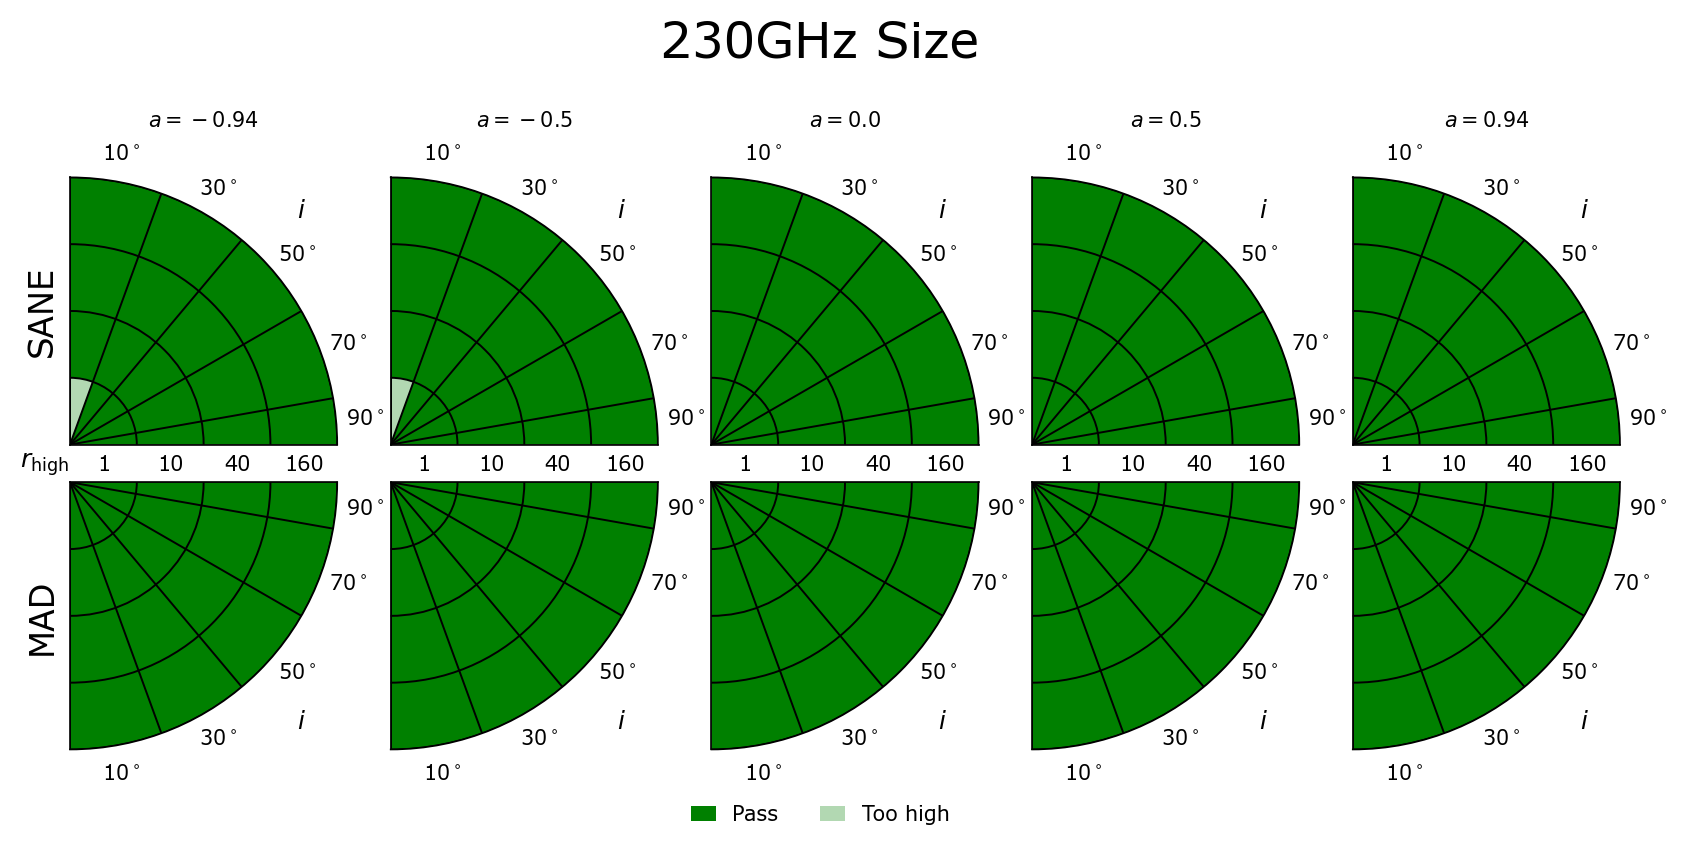
\includegraphics[width=0.8\textwidth]{./figures/230GHz_size_Constraints.png}
  \caption{2nd Moment Constraint}
  \label{fig:230GHz_size_pizza}
\end{figure*}
\begin{figure*}
  \centering
  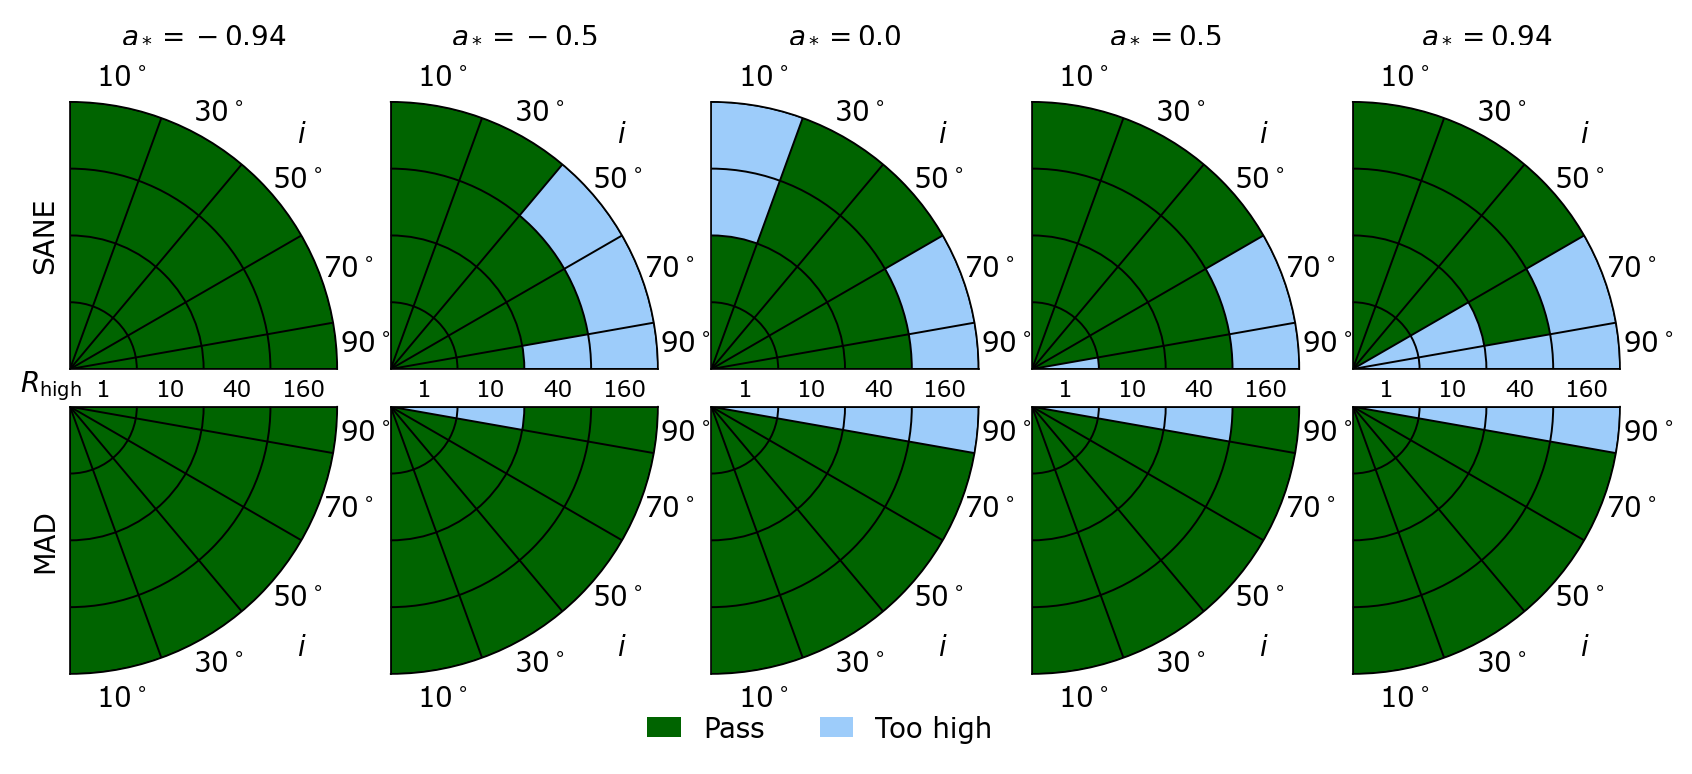
\includegraphics[width=0.8\textwidth]{./figures/Null_loc_Constraints.png}
  \caption{Null Location Constraint}
  \label{fig:null_pizza}
\end{figure*}
\begin{figure*}
  \centering
  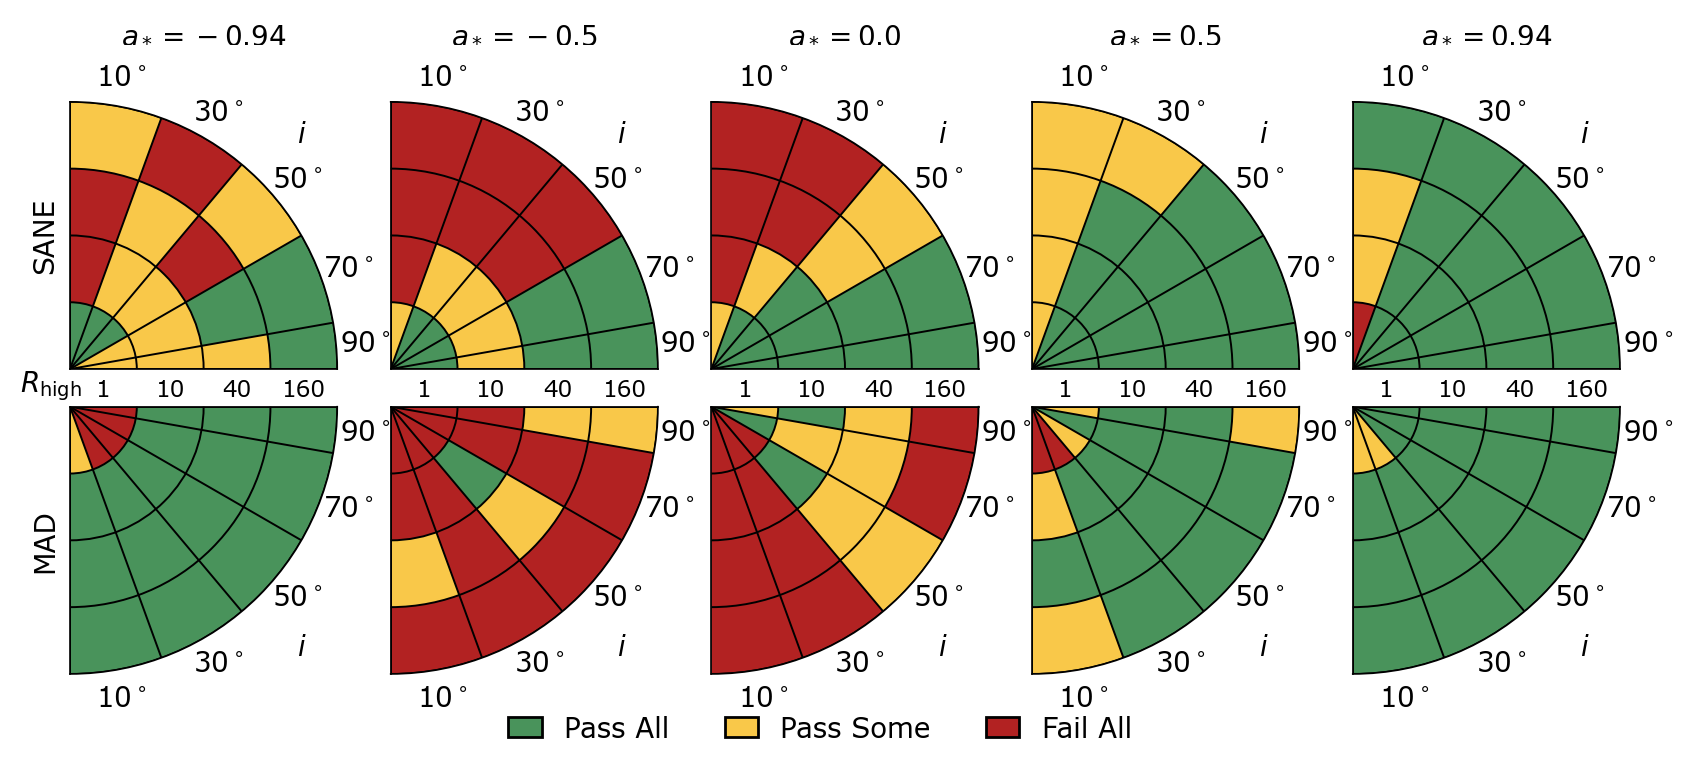
\includegraphics[width=0.8\textwidth]{./figures/Mring_d_Constraints.png}
  \caption{M-ring Diameter Constraints}
  \label{fig:mring_diam_pizza}
\end{figure*}
\begin{figure*}
  \centering
  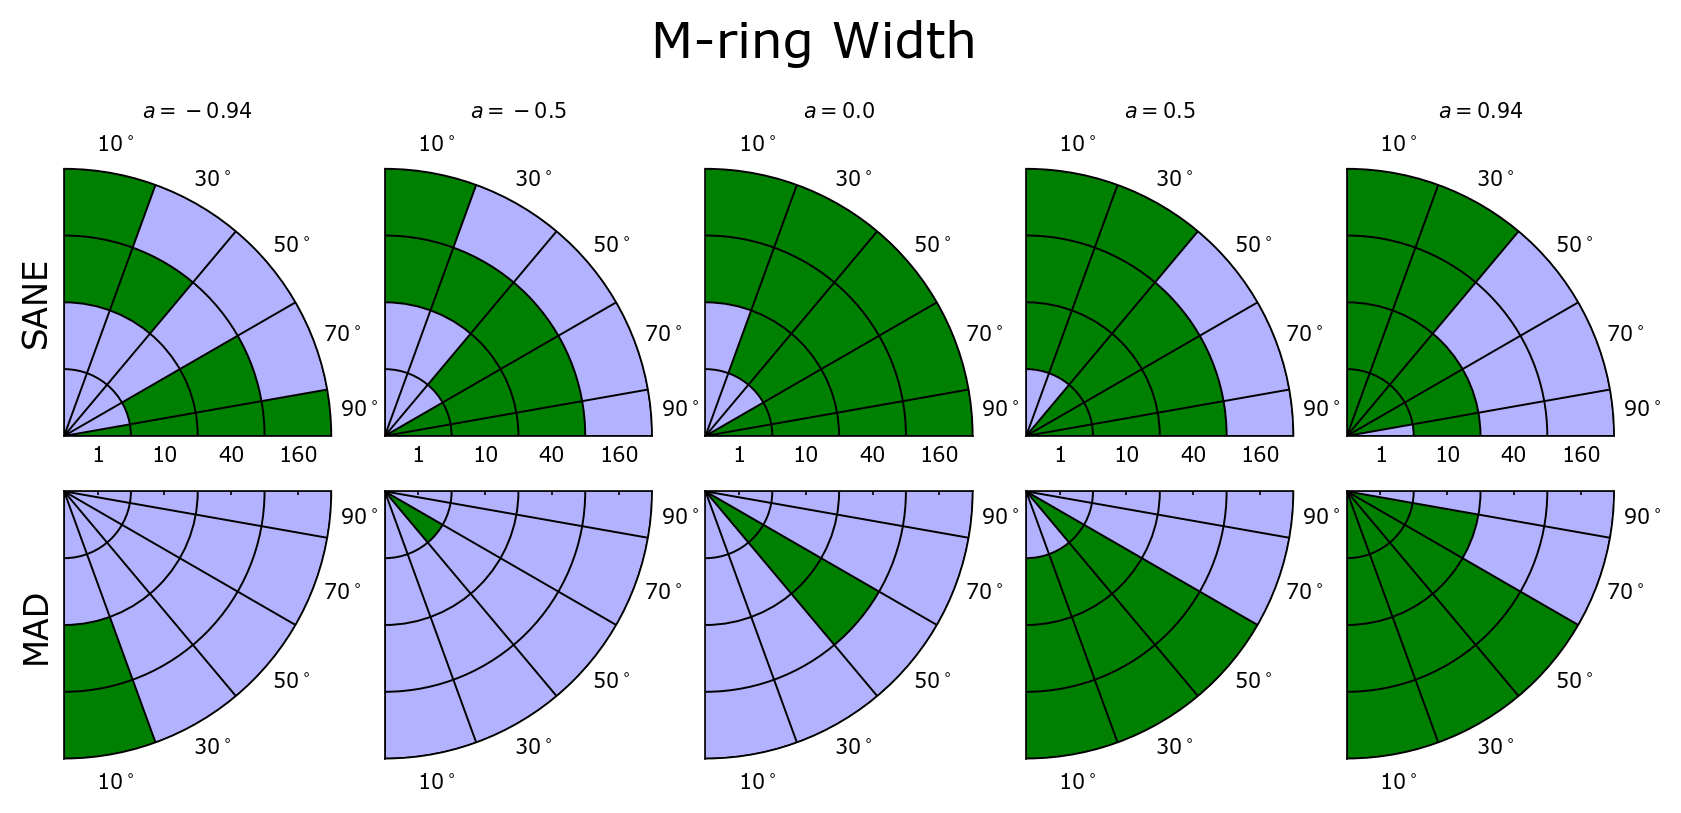
\includegraphics[width=0.8\textwidth]{./figures/Mring_w_Constraints.png}
  \caption{M-ring Width Constraints}
  \label{fig:mring_width_pizza}
\end{figure*}
\begin{figure*}
  \centering
  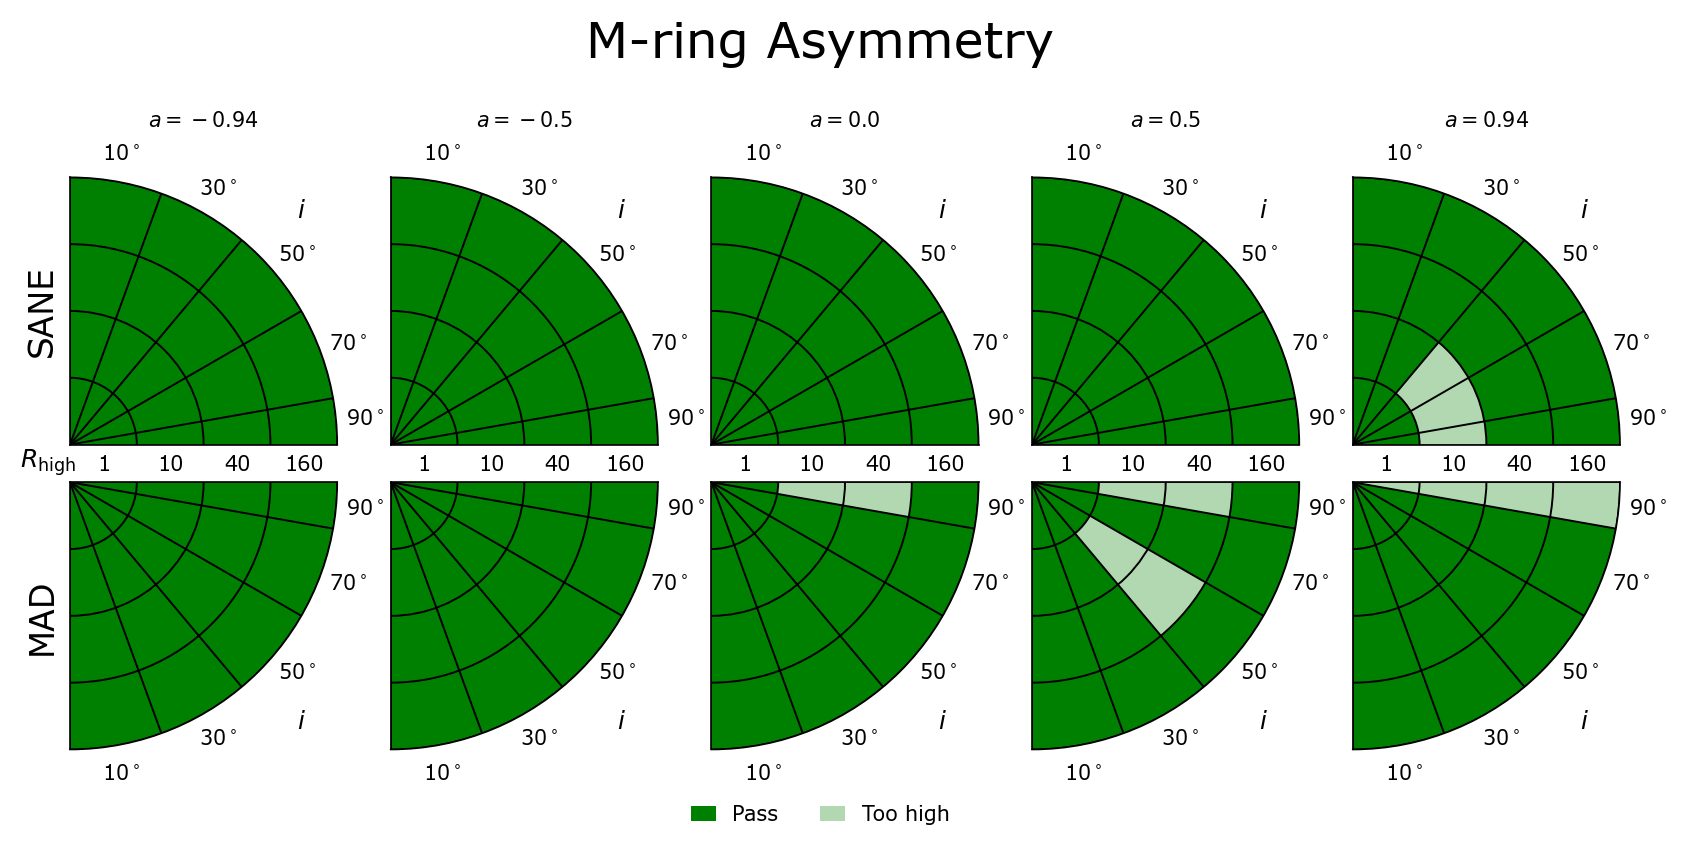
\includegraphics[width=0.8\textwidth]{./figures/Mring_f1_Constraints.png}
  \caption{M-ring Asymmetry Constraints}
  \label{fig:mring_asymm_pizza}
\end{figure*}
\begin{figure*}
  \centering
  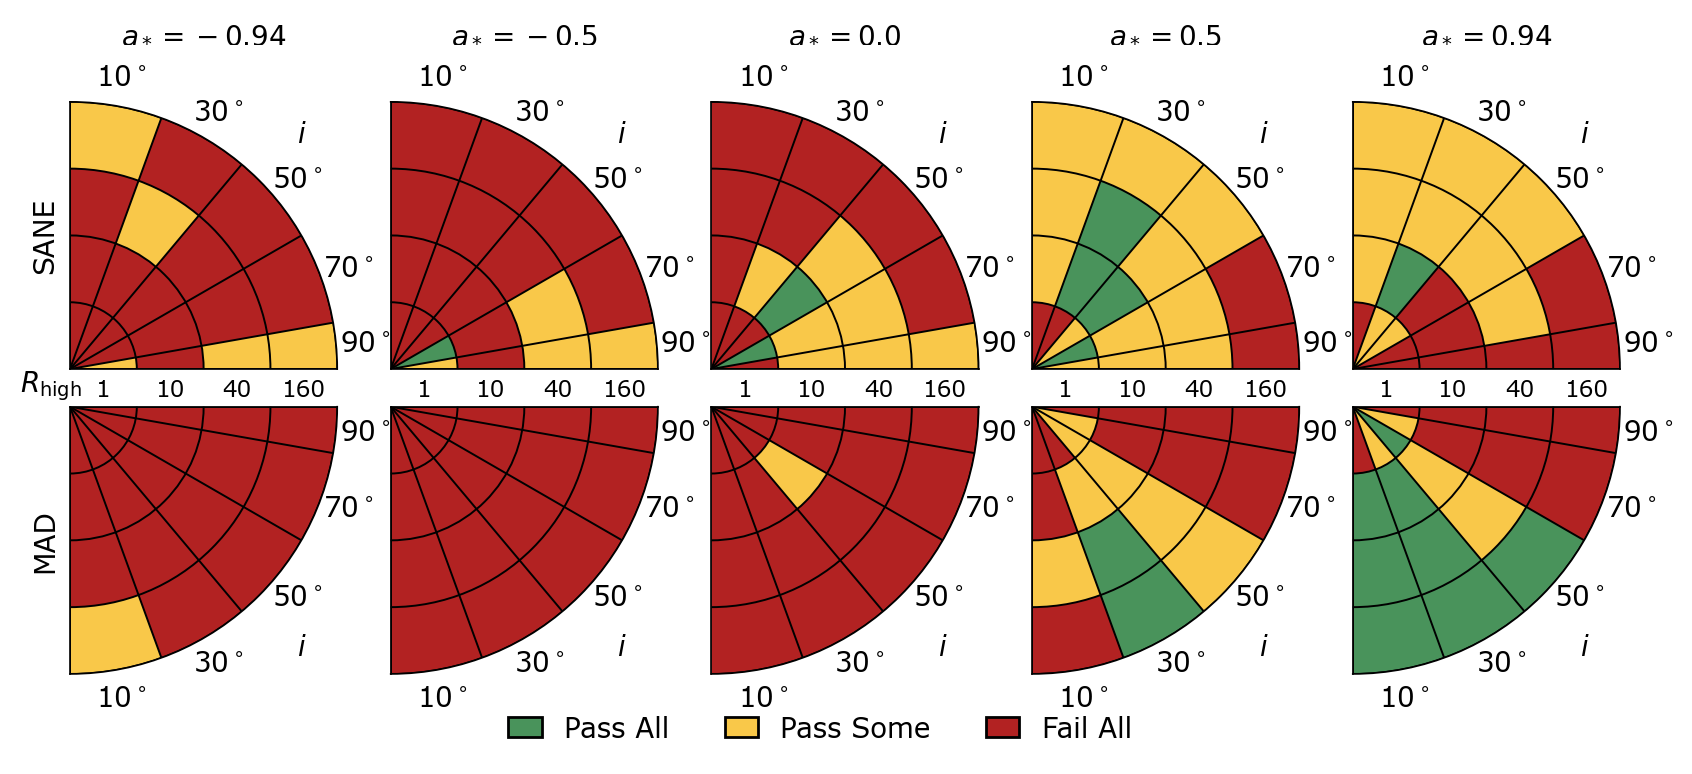
\includegraphics[width=0.8\textwidth]{./figures/Interferometric_Constraints.png}
  \caption{Combined EHT Constraints}
  \label{fig:eht_comb_pizza}
\end{figure*}

Then the non-EHT constraints.

\begin{figure*}
  \centering
  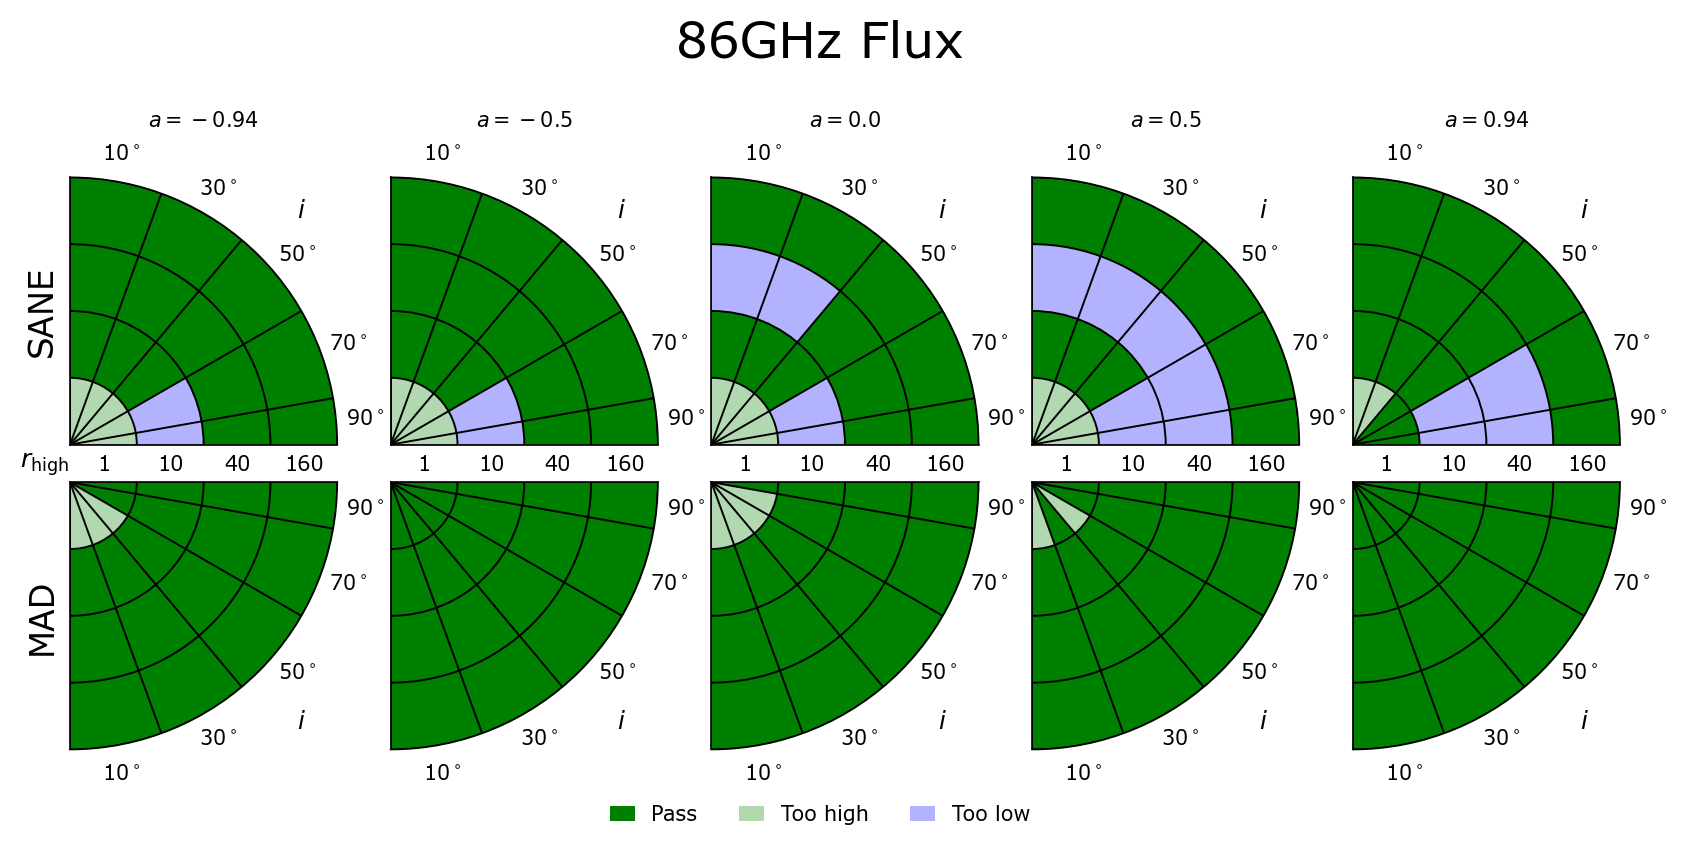
\includegraphics[width=0.8\textwidth]{./figures/86GHz_flux_Constraints.png}
  \caption{86GHz Flux Constraints}
  \label{fig:86GHz_flux_pizza}
\end{figure*}

\begin{figure*}
  \centering
  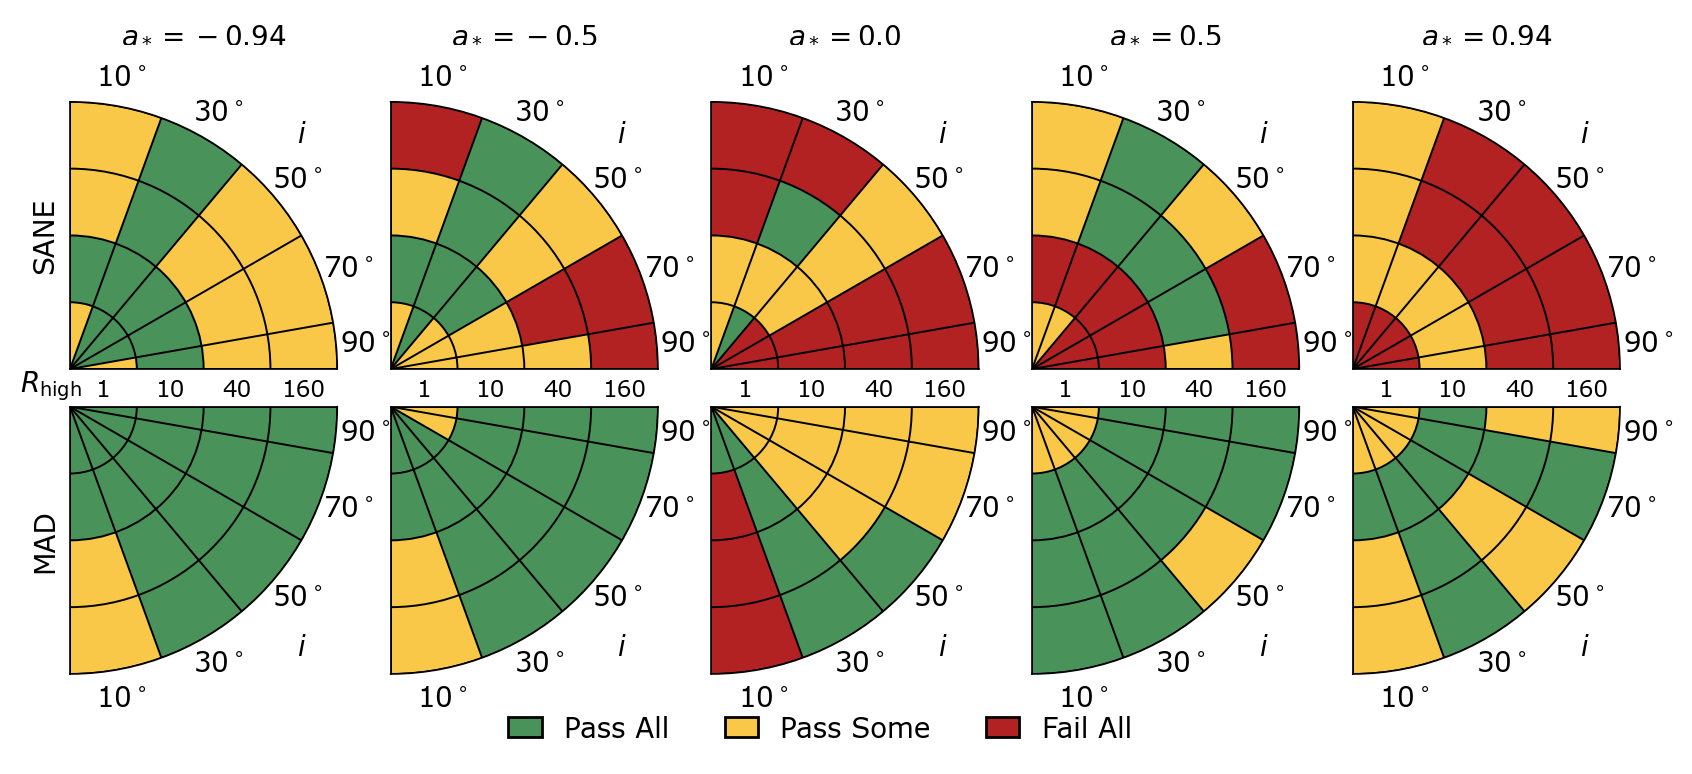
\includegraphics[width=0.8\textwidth]{./figures/86GHz_size_Constraints.png}
  \caption{86GHz Size Constraints}
  \label{fig:86GHz_size_pizza}
\end{figure*}
\begin{figure*}
  \centering
  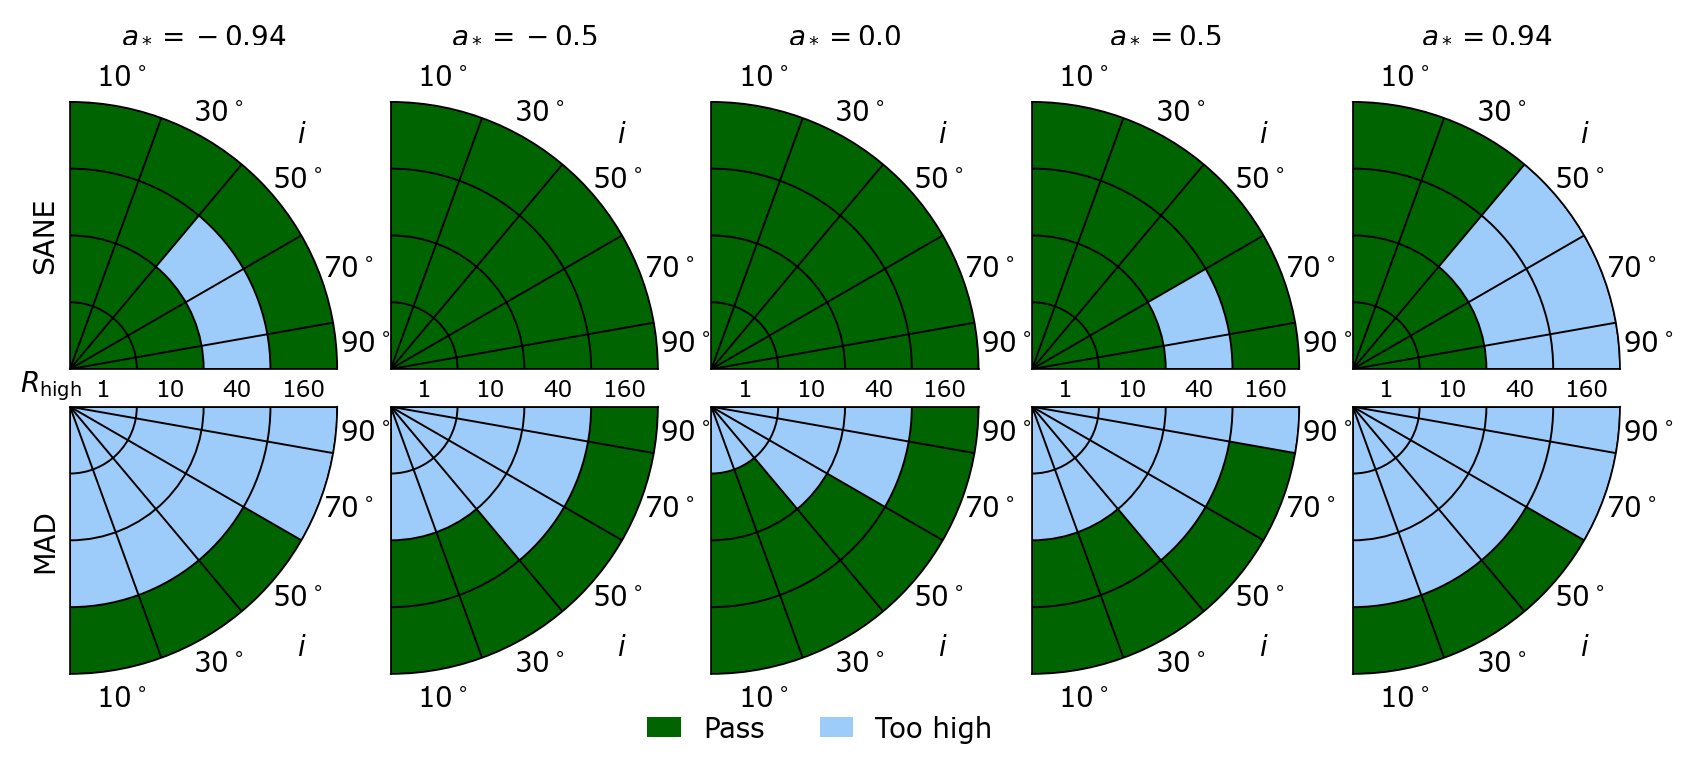
\includegraphics[width=0.8\textwidth]{./figures/2um_flux_Constraints.png}
  \caption{$2.2\mu$m Flux Constraints}
  \label{fig:2um_flux_pizza}
\end{figure*}
\begin{figure*}
  \centering
  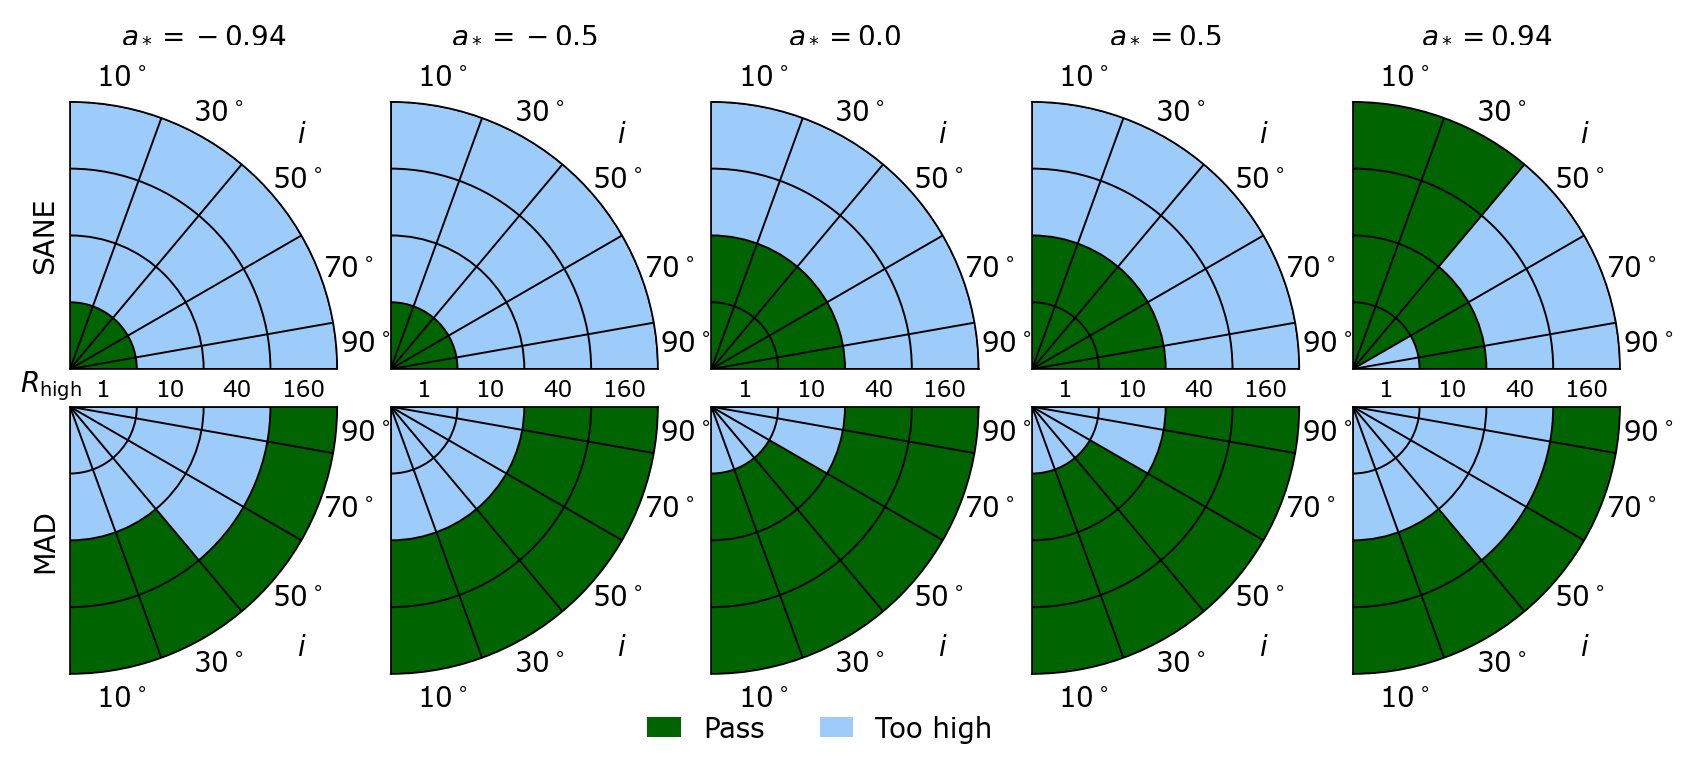
\includegraphics[width=0.8\textwidth]{./figures/Xray_flux_Constraints.png}
  \caption{X-Ray Luminosity Constraints}
  \label{fig:xray_pizza}
\end{figure*}
\begin{figure*}
  \centering
  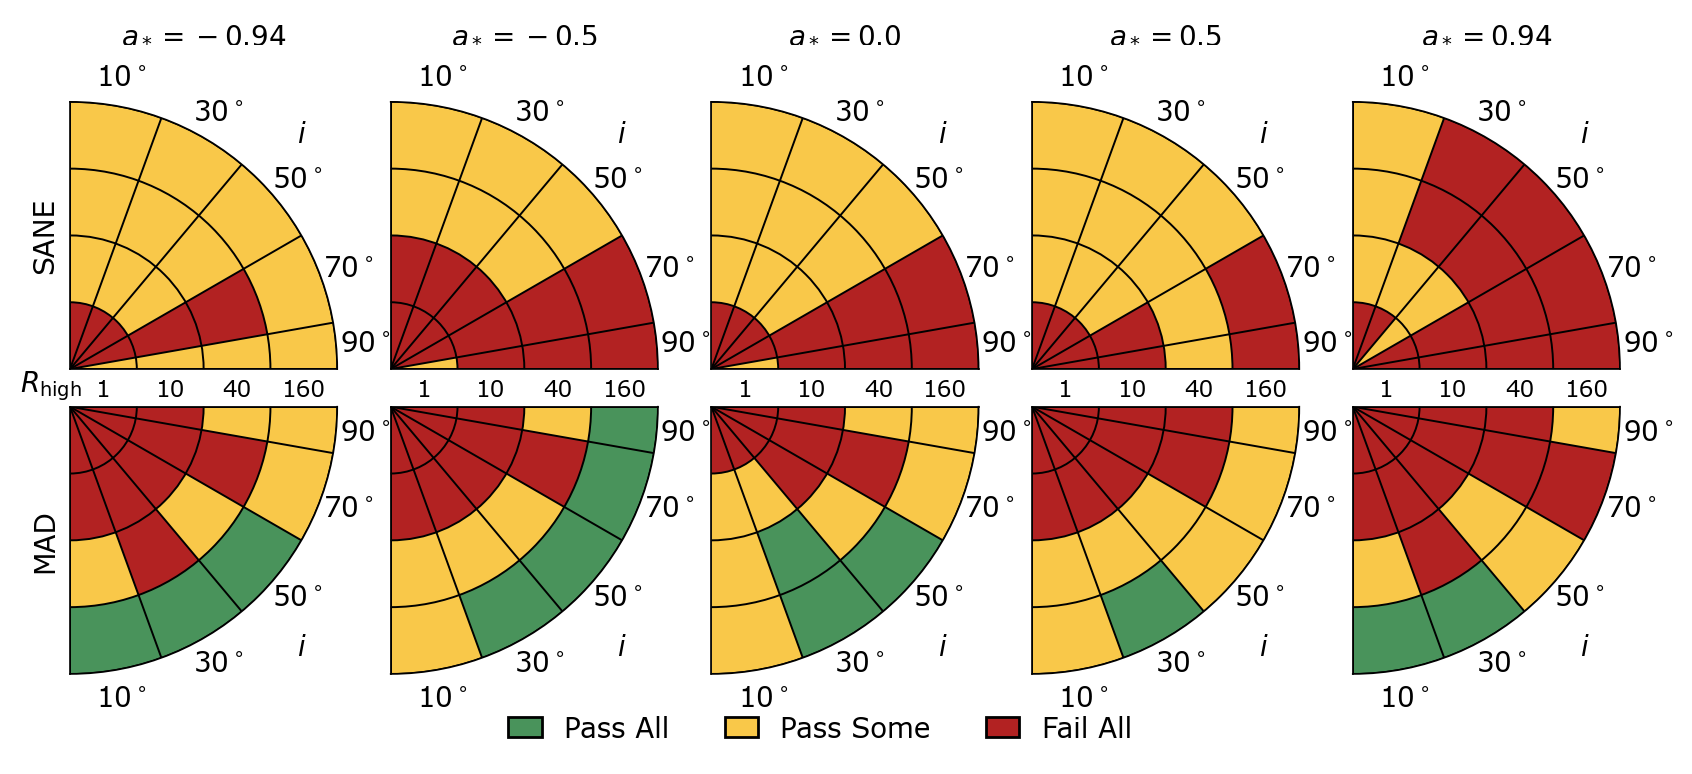
\includegraphics[width=0.8\textwidth]{./figures/Non_Interferometric_Constraints.png}
  \caption{Combined non-EHT Constraints}
  \label{fig:noneht_pizza}
\end{figure*}

Then the full set of combined constraints, without variability.

\begin{figure*}
  \centering
  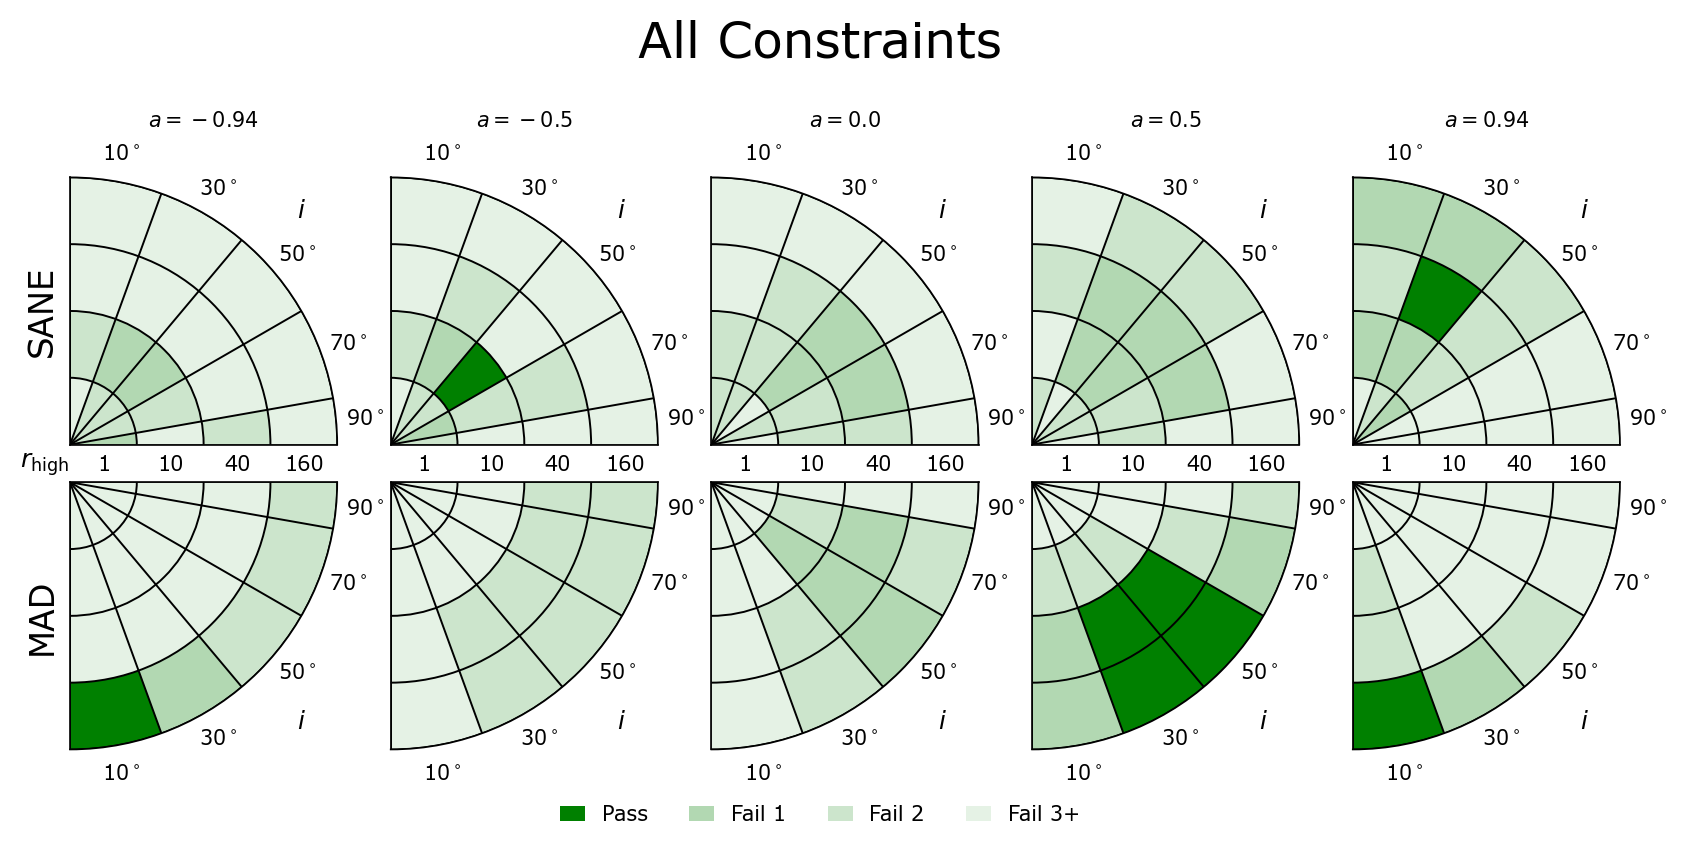
\includegraphics[width=0.8\textwidth]{./figures/All_Constraints.png}
  \caption{Combined constraints without structural or flux variability.}
  \label{fig:all_pizza}
\end{figure*}

Then the variability constraints.

\begin{figure*}
  \centering
  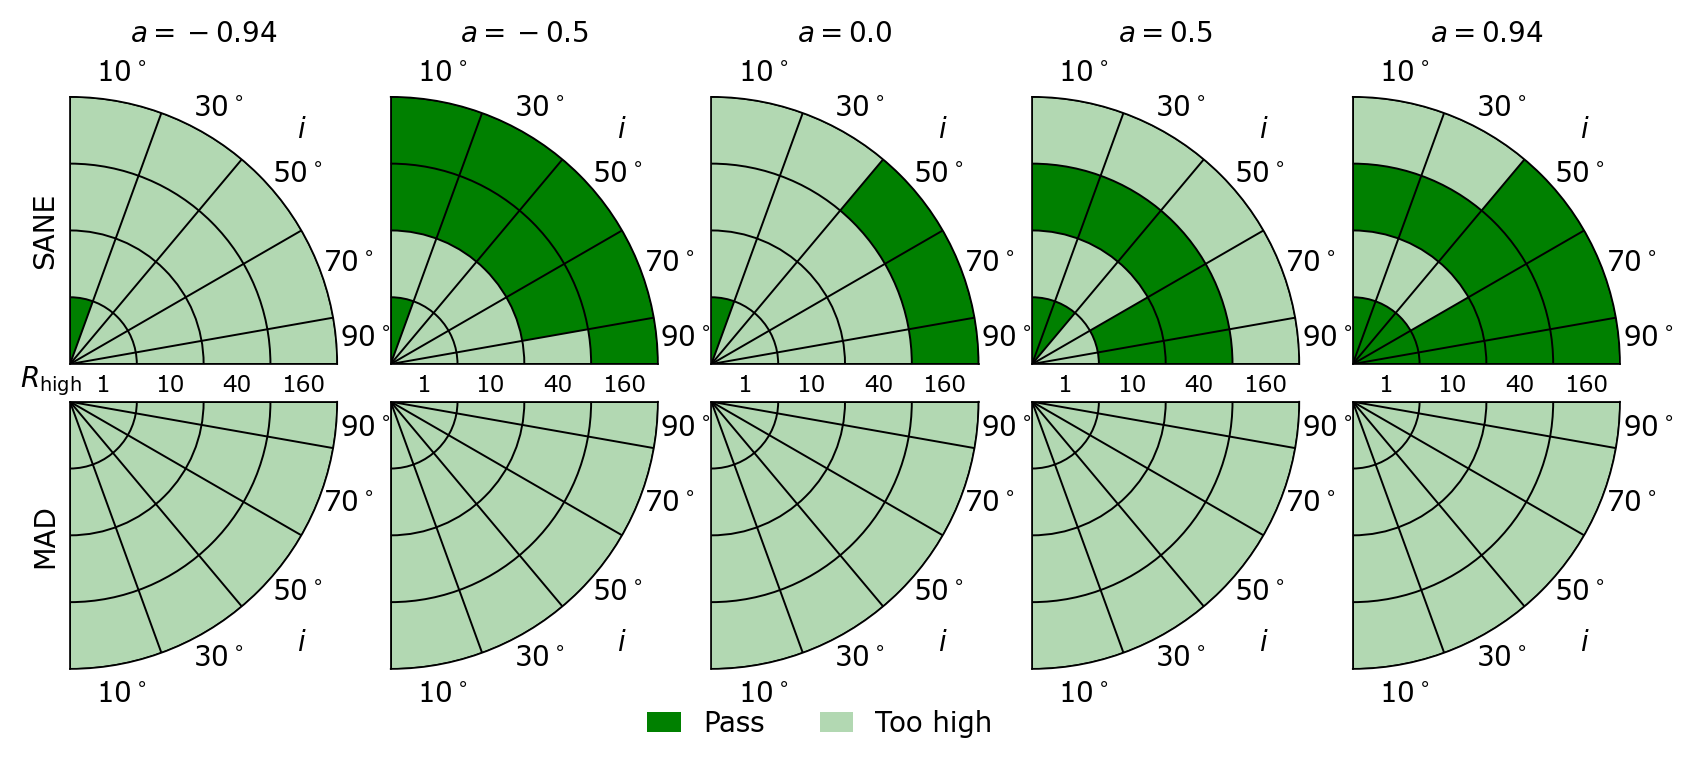
\includegraphics[width=0.8\textwidth]{./figures/230GHz_3Hr_MI_Constraints.png}
  \caption{$M_3$ Constraints}
  \label{fig:m3_pizza}
\end{figure*}

\begin{figure*}
  \centering
  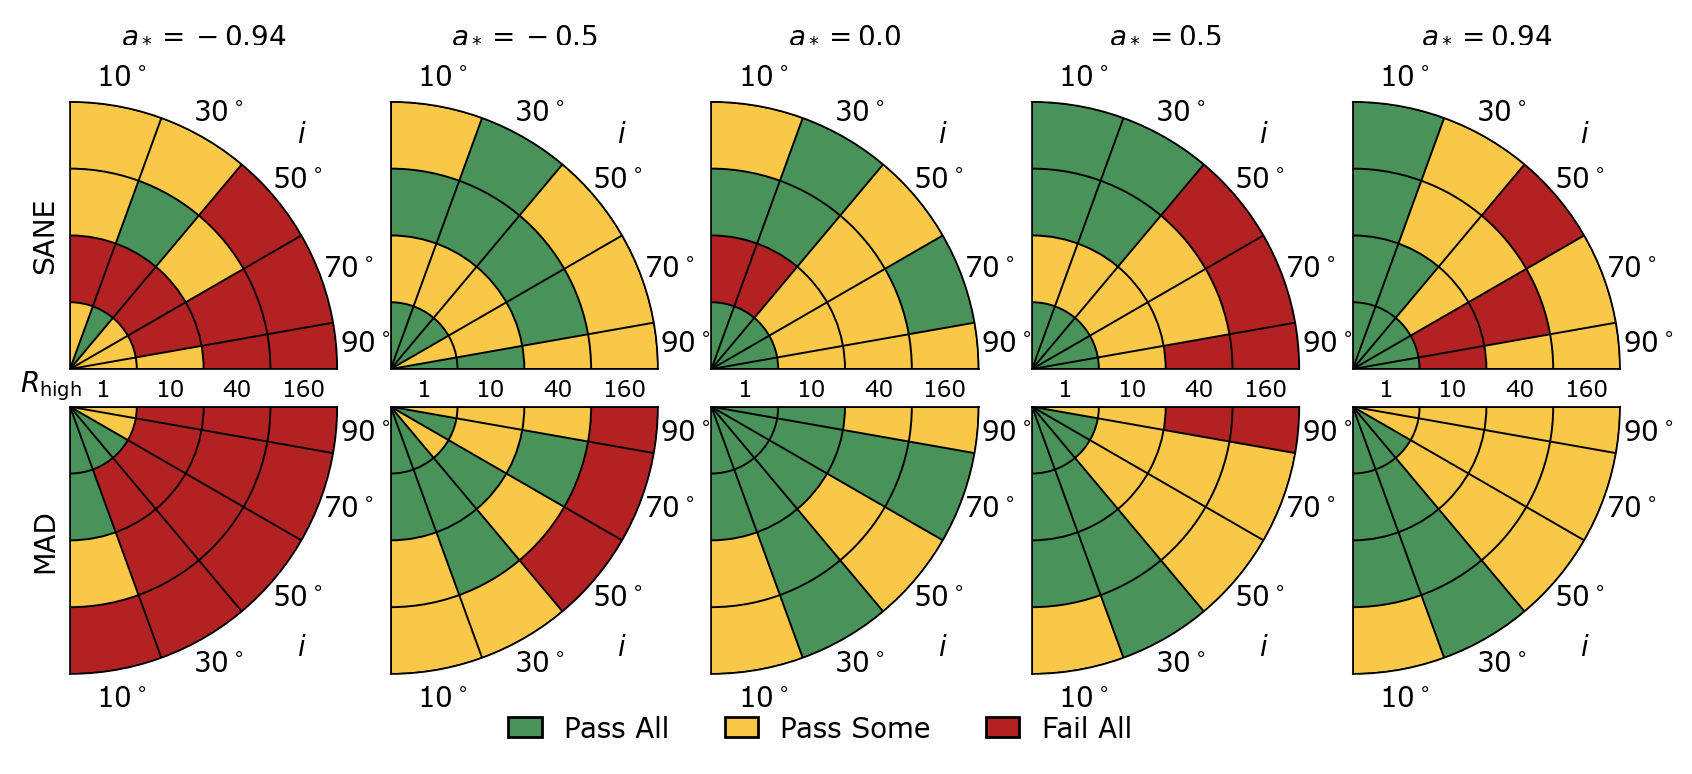
\includegraphics[width=0.8\textwidth]{./figures/4Glam_Constraints.png}
  \caption{EHT Structural Variability Constraints}
  \label{fig:ehtvar_pizza}
\end{figure*}

Tables are available for all model sets.

\clearpage


%\startlongtable
\begin{deluxetable*}{cccc|cccc|c|ccccc|c|c|cc|cccc}
\tabletypesize{\scriptsize}
\tablecaption{Pass/Fail Table, Illinois Thermal Models}
\label{tab:illinoisPF}
\tablehead{ \colhead{M/S}  &  %
\colhead{Spin}  &  %
\colhead{$i$}  &  %
\colhead{$\Rh$}  &  %
\colhead{$F_{86}$}  &  %
\colhead{$\lambda_{maj,86}$}  &  %
\colhead{$F_{2\mu{\rm m}}$}  &  %
\colhead{$L_X$}  &  %
\colhead{non-EHT}  &  %
\colhead{$\lambda_{230}$}  &  %
\colhead{Nulls}  &  %
\colhead{Ring D}  &  %
\colhead{Ring W}  &  %
\colhead{Ring A}  &  %
\colhead{EHT}  &  %
\colhead{All}  &  %
\colhead{MI} & %
\colhead{4G$\lambda$} & %
\colhead{$\dot{M}/\dot{M}_{Edd}$}  &  %
\colhead{$L_{bol}/(\dot{M} c^{2})$}  &  %
\colhead{$P_{out}$(cgs)}  &  %
\colhead{$P_{out}/(\dot{M} c^2)$}}
\startdata
S & -0.94 & 10.0 & 1.0 & Fail & Fail & Pass & Pass & Fail & Fail & Pass & Pass & Fail & Pass & Fail & Fail & Pass & Pass &1.75$\times10^{-7}$ & 1.33$\times10^{-4}$ & 2.21$\times10^{36}$ & 2.46$\times10^{-3}$\\
S & -0.94 & 10.0 & 10.0 & Pass & Pass & Pass & Fail & Fail & Pass & Pass & Fail & Fail & Pass & Fail & Fail & Fail & Fail &2.09$\times10^{-6}$ & 3.35$\times10^{-5}$ & 2.67$\times10^{37}$ & 2.46$\times10^{-3}$\\
S & -0.94 & 10.0 & 40.0 & Pass & Fail & Pass & Fail & Fail & Pass & Pass & Fail & Fail & Pass & Fail & Fail & Fail & Pass &7.75$\times10^{-6}$ & 2.40$\times10^{-5}$ & 9.90$\times10^{37}$ & 2.46$\times10^{-3}$\\
S & -0.94 & 10.0 & 160.0 & Pass & Fail & Pass & Fail & Fail & Pass & Pass & Fail & Fail & Pass & Fail & Fail & Fail & Pass &1.35$\times10^{-5}$ & 1.19$\times10^{-5}$ & 1.71$\times10^{38}$ & 2.46$\times10^{-3}$\\
S & -0.94 & 30.0 & 1.0 & Fail & Pass & Pass & Pass & Fail & Pass & Pass & Pass & Fail & Pass & Fail & Fail & Fail & Pass &1.68$\times10^{-7}$ & 1.28$\times10^{-4}$ & 2.12$\times10^{36}$ & 2.46$\times10^{-3}$\\
S & -0.94 & 30.0 & 10.0 & Pass & Pass & Pass & Fail & Fail & Pass & Pass & Pass & Fail & Pass & Fail & Fail & Fail & Fail &2.01$\times10^{-6}$ & 3.22$\times10^{-5}$ & 2.56$\times10^{37}$ & 2.46$\times10^{-3}$\\
S & -0.94 & 30.0 & 40.0 & Pass & Pass & Pass & Fail & Fail & Pass & Pass & Fail & Pass & Pass & Fail & Fail & Fail & Pass &8.14$\times10^{-6}$ & 2.53$\times10^{-5}$ & 1.04$\times10^{38}$ & 2.46$\times10^{-3}$\\
S & -0.94 & 30.0 & 160.0 & Pass & Pass & Pass & Fail & Fail & Pass & Pass & Fail & Fail & Pass & Fail & Fail & Fail & Pass &1.48$\times10^{-5}$ & 1.29$\times10^{-5}$ & 1.86$\times10^{38}$ & 2.46$\times10^{-3}$\\
S & -0.94 & 50.0 & 1.0 & Fail & Pass & Pass & Pass & Fail & Pass & Pass & Pass & Fail & Pass & Fail & Fail & Fail & Fail &1.64$\times10^{-7}$ & 1.25$\times10^{-4}$ & 2.06$\times10^{36}$ & 2.46$\times10^{-3}$\\
S & -0.94 & 50.0 & 10.0 & Pass & Pass & Pass & Fail & Fail & Pass & Pass & Pass & Fail & Pass & Fail & Fail & Fail & Fail &1.98$\times10^{-6}$ & 3.18$\times10^{-5}$ & 2.53$\times10^{37}$ & 2.46$\times10^{-3}$\\
S & -0.94 & 50.0 & 40.0 & Pass & Fail & Fail & Fail & Fail & Pass & Pass & Fail & Fail & Pass & Fail & Fail & Fail & Pass &8.47$\times10^{-6}$ & 2.62$\times10^{-5}$ & 1.08$\times10^{38}$ & 2.46$\times10^{-3}$\\
S & -0.94 & 50.0 & 160.0 & Pass & Fail & Pass & Fail & Fail & Pass & Pass & Pass & Fail & Pass & Fail & Fail & Fail & Fail &1.57$\times10^{-5}$ & 1.37$\times10^{-5}$ & 1.99$\times10^{38}$ & 2.46$\times10^{-3}$\\
S & -0.94 & 70.0 & 1.0 & Fail & Pass & Pass & Pass & Fail & Pass & Pass & Pass & Fail & Pass & Fail & Fail & Fail & Fail &1.71$\times10^{-7}$ & 1.30$\times10^{-4}$ & 2.15$\times10^{36}$ & 2.46$\times10^{-3}$\\
S & -0.94 & 70.0 & 10.0 & Pass & Pass & Pass & Fail & Fail & Pass & Pass & Fail & Fail & Pass & Fail & Fail & Fail & Fail &2.19$\times10^{-6}$ & 3.50$\times10^{-5}$ & 2.80$\times10^{37}$ & 2.46$\times10^{-3}$\\
S & -0.94 & 70.0 & 40.0 & Pass & Fail & Fail & Fail & Fail & Pass & Pass & Pass & Fail & Pass & Fail & Fail & Fail & Fail &8.78$\times10^{-6}$ & 2.71$\times10^{-5}$ & 1.12$\times10^{38}$ & 2.46$\times10^{-3}$\\
S & -0.94 & 70.0 & 160.0 & Pass & Fail & Pass & Fail & Fail & Pass & Pass & Pass & Fail & Pass & Fail & Fail & Fail & Fail &1.68$\times10^{-5}$ & 1.47$\times10^{-5}$ & 2.12$\times10^{38}$ & 2.46$\times10^{-3}$\\
S & -0.94 & 90.0 & 1.0 & Fail & Pass & Pass & Pass & Fail & Pass & Pass & Pass & Pass & Pass & Pass & Fail & Fail & Pass &1.71$\times10^{-7}$ & 1.30$\times10^{-4}$ & 2.15$\times10^{36}$ & 2.46$\times10^{-3}$\\
S & -0.94 & 90.0 & 10.0 & Fail & Pass & Pass & Fail & Fail & Pass & Pass & Fail & Fail & Pass & Fail & Fail & Fail & Pass &2.29$\times10^{-6}$ & 3.64$\times10^{-5}$ & 2.92$\times10^{37}$ & 2.46$\times10^{-3}$\\
S & -0.94 & 90.0 & 40.0 & Pass & Fail & Fail & Fail & Fail & Pass & Pass & Pass & Pass & Pass & Pass & Fail & Fail & Fail &9.16$\times10^{-6}$ & 2.82$\times10^{-5}$ & 1.17$\times10^{38}$ & 2.46$\times10^{-3}$\\
S & -0.94 & 90.0 & 160.0 & Pass & Fail & Pass & Fail & Fail & Pass & Pass & Pass & Fail & Pass & Fail & Fail & Fail & Fail &1.79$\times10^{-5}$ & 1.56$\times10^{-5}$ & 2.27$\times10^{38}$ & 2.46$\times10^{-3}$\\
S & -0.5 & 10.0 & 1.0 & Fail & Pass & Pass & Pass & Fail & Fail & Pass & Pass & Fail & Pass & Fail & Fail & Pass & Pass &1.05$\times10^{-7}$ & 2.26$\times10^{-4}$ & 1.89$\times10^{35}$ & 3.53$\times10^{-4}$\\
S & -0.5 & 10.0 & 10.0 & Pass & Pass & Pass & Fail & Fail & Pass & Pass & Fail & Fail & Pass & Fail & Fail & Fail & Fail &1.16$\times10^{-6}$ & 3.65$\times10^{-5}$ & 2.08$\times10^{36}$ & 3.53$\times10^{-4}$\\
S & -0.5 & 10.0 & 40.0 & Pass & Fail & Pass & Fail & Fail & Pass & Pass & Fail & Pass & Pass & Fail & Fail & Pass & Pass &6.87$\times10^{-6}$ & 2.84$\times10^{-5}$ & 1.18$\times10^{37}$ & 3.53$\times10^{-4}$\\
S & -0.5 & 10.0 & 160.0 & Pass & Fail & Pass & Fail & Fail & Pass & Pass & Fail & Pass & Pass & Fail & Fail & Pass & Pass &1.11$\times10^{-5}$ & 1.25$\times10^{-5}$ & 1.90$\times10^{37}$ & 3.53$\times10^{-4}$\\
S & -0.5 & 30.0 & 1.0 & Fail & Pass & Pass & Pass & Fail & Pass & Pass & Pass & Fail & Pass & Fail & Fail & Fail & Pass &1.01$\times10^{-7}$ & 2.17$\times10^{-4}$ & 1.81$\times10^{35}$ & 3.53$\times10^{-4}$\\
S & -0.5 & 30.0 & 10.0 & Pass & Pass & Pass & Fail & Fail & Pass & Pass & Pass & Fail & Pass & Fail & Fail & Fail & Fail &1.09$\times10^{-6}$ & 3.46$\times10^{-5}$ & 1.96$\times10^{36}$ & 3.53$\times10^{-4}$\\
S & -0.5 & 30.0 & 40.0 & Pass & Pass & Pass & Fail & Fail & Pass & Pass & Fail & Pass & Pass & Fail & Fail & Pass & Pass &6.93$\times10^{-6}$ & 2.85$\times10^{-5}$ & 1.18$\times10^{37}$ & 3.53$\times10^{-4}$\\
S & -0.5 & 30.0 & 160.0 & Pass & Pass & Pass & Fail & Fail & Pass & Pass & Fail & Fail & Pass & Fail & Fail & Pass & Pass &1.13$\times10^{-5}$ & 1.26$\times10^{-5}$ & 1.92$\times10^{37}$ & 3.53$\times10^{-4}$\\
S & -0.5 & 50.0 & 1.0 & Fail & Pass & Pass & Pass & Fail & Pass & Pass & Pass & Fail & Pass & Fail & Fail & Fail & Pass &9.75$\times10^{-8}$ & 2.11$\times10^{-4}$ & 1.75$\times10^{35}$ & 3.53$\times10^{-4}$\\
S & -0.5 & 50.0 & 10.0 & Pass & Pass & Pass & Fail & Fail & Pass & Pass & Pass & Fail & Pass & Fail & Fail & Fail & Fail &1.10$\times10^{-6}$ & 3.48$\times10^{-5}$ & 1.97$\times10^{36}$ & 3.53$\times10^{-4}$\\
S & -0.5 & 50.0 & 40.0 & Pass & Fail & Pass & Fail & Fail & Pass & Pass & Fail & Fail & Pass & Fail & Fail & Pass & Pass &6.55$\times10^{-6}$ & 2.70$\times10^{-5}$ & 1.12$\times10^{37}$ & 3.53$\times10^{-4}$\\
S & -0.5 & 50.0 & 160.0 & Pass & Pass & Pass & Fail & Fail & Pass & Fail & Fail & Fail & Pass & Fail & Fail & Pass & Pass &1.10$\times10^{-5}$ & 1.22$\times10^{-5}$ & 1.85$\times10^{37}$ & 3.53$\times10^{-4}$\\
S & -0.5 & 70.0 & 1.0 & Fail & Pass & Pass & Pass & Fail & Pass & Pass & Pass & Pass & Pass & Pass & Fail & Fail & Fail &9.96$\times10^{-8}$ & 2.14$\times10^{-4}$ & 1.78$\times10^{35}$ & 3.53$\times10^{-4}$\\
S & -0.5 & 70.0 & 10.0 & Fail & Pass & Pass & Fail & Fail & Pass & Pass & Pass & Fail & Pass & Fail & Fail & Fail & Fail &1.18$\times10^{-6}$ & 3.71$\times10^{-5}$ & 2.12$\times10^{36}$ & 3.53$\times10^{-4}$\\
S & -0.5 & 70.0 & 40.0 & Pass & Fail & Pass & Fail & Fail & Pass & Pass & Pass & Pass & Pass & Pass & Fail & Pass & Pass &6.41$\times10^{-6}$ & 2.63$\times10^{-5}$ & 1.08$\times10^{37}$ & 3.53$\times10^{-4}$\\
S & -0.5 & 70.0 & 160.0 & Pass & Fail & Pass & Fail & Fail & Pass & Fail & Pass & Fail & Pass & Fail & Fail & Pass & Fail &1.13$\times10^{-5}$ & 1.24$\times10^{-5}$ & 1.89$\times10^{37}$ & 3.53$\times10^{-4}$\\
S & -0.5 & 90.0 & 1.0 & Fail & Fail & Pass & Pass & Fail & Pass & Pass & Pass & Pass & Pass & Pass & Fail & Fail & Pass &1.00$\times10^{-7}$ & 2.15$\times10^{-4}$ & 1.79$\times10^{35}$ & 3.53$\times10^{-4}$\\
S & -0.5 & 90.0 & 10.0 & Fail & Pass & Pass & Fail & Fail & Pass & Pass & Pass & Fail & Pass & Fail & Fail & Fail & Pass &1.27$\times10^{-6}$ & 3.96$\times10^{-5}$ & 2.27$\times10^{36}$ & 3.53$\times10^{-4}$\\
S & -0.5 & 90.0 & 40.0 & Pass & Fail & Pass & Fail & Fail & Pass & Fail & Pass & Pass & Pass & Fail & Fail & Fail & Fail &6.36$\times10^{-6}$ & 2.61$\times10^{-5}$ & 1.08$\times10^{37}$ & 3.53$\times10^{-4}$\\
S & -0.5 & 90.0 & 160.0 & Pass & Fail & Pass & Fail & Fail & Pass & Fail & Pass & Fail & Pass & Fail & Fail & Pass & Fail &1.14$\times10^{-5}$ & 1.24$\times10^{-5}$ & 1.89$\times10^{37}$ & 3.53$\times10^{-4}$\\
S & 0.0 & 10.0 & 1.0 & Fail & Pass & Pass & Pass & Fail & Fail & Pass & Pass & Fail & Pass & Fail & Fail & Pass & Pass &5.80$\times10^{-8}$ & 4.53$\times10^{-4}$ & 1.17$\times10^{35}$ & 3.96$\times10^{-4}$\\
S & 0.0 & 10.0 & 10.0 & Pass & Pass & Pass & Pass & Pass & Pass & Pass & Fail & Fail & Pass & Fail & Fail & Fail & Fail &5.07$\times10^{-7}$ & 6.62$\times10^{-5}$ & 1.05$\times10^{36}$ & 3.96$\times10^{-4}$\\
S & 0.0 & 10.0 & 40.0 & Fail & Fail & Pass & Fail & Fail & Pass & Fail & Fail & Pass & Pass & Fail & Fail & Fail & Pass &2.70$\times10^{-6}$ & 3.91$\times10^{-5}$ & 5.60$\times10^{36}$ & 3.96$\times10^{-4}$\\
S & 0.0 & 10.0 & 160.0 & Pass & Fail & Pass & Fail & Fail & Pass & Fail & Fail & Pass & Pass & Fail & Fail & Fail & Pass &4.62$\times10^{-6}$ & 1.69$\times10^{-5}$ & 8.94$\times10^{36}$ & 3.96$\times10^{-4}$\\
S & 0.0 & 30.0 & 1.0 & Fail & Pass & Pass & Pass & Fail & Pass & Pass & Pass & Fail & Pass & Fail & Fail & Fail & Pass &5.50$\times10^{-8}$ & 4.32$\times10^{-4}$ & 1.11$\times10^{35}$ & 3.96$\times10^{-4}$\\
S & 0.0 & 30.0 & 10.0 & Pass & Fail & Pass & Pass & Fail & Pass & Pass & Pass & Fail & Pass & Fail & Fail & Fail & Fail &4.79$\times10^{-7}$ & 6.29$\times10^{-5}$ & 9.93$\times10^{35}$ & 3.96$\times10^{-4}$\\
S & 0.0 & 30.0 & 40.0 & Fail & Fail & Pass & Fail & Fail & Pass & Pass & Fail & Pass & Pass & Fail & Fail & Fail & Pass &2.60$\times10^{-6}$ & 3.79$\times10^{-5}$ & 5.36$\times10^{36}$ & 3.96$\times10^{-4}$\\
S & 0.0 & 30.0 & 160.0 & Pass & Fail & Pass & Fail & Fail & Pass & Pass & Fail & Fail & Pass & Fail & Fail & Fail & Pass &4.32$\times10^{-6}$ & 1.59$\times10^{-5}$ & 8.38$\times10^{36}$ & 3.96$\times10^{-4}$\\
S & 0.0 & 50.0 & 1.0 & Fail & Fail & Pass & Pass & Fail & Pass & Pass & Pass & Fail & Pass & Fail & Fail & Fail & Pass &5.29$\times10^{-8}$ & 4.16$\times10^{-4}$ & 1.06$\times10^{35}$ & 3.96$\times10^{-4}$\\
S & 0.0 & 50.0 & 10.0 & Pass & Fail & Pass & Pass & Fail & Pass & Pass & Pass & Pass & Pass & Pass & Fail & Fail & Fail &4.66$\times10^{-7}$ & 6.13$\times10^{-5}$ & 9.67$\times10^{35}$ & 3.96$\times10^{-4}$\\
S & 0.0 & 50.0 & 40.0 & Pass & Pass & Pass & Fail & Fail & Pass & Pass & Pass & Pass & Pass & Pass & Fail & Fail & Fail &2.72$\times10^{-6}$ & 3.96$\times10^{-5}$ & 5.69$\times10^{36}$ & 3.96$\times10^{-4}$\\
S & 0.0 & 50.0 & 160.0 & Pass & Pass & Pass & Fail & Fail & Pass & Pass & Pass & Fail & Pass & Fail & Fail & Pass & Pass &4.71$\times10^{-6}$ & 1.73$\times10^{-5}$ & 9.32$\times10^{36}$ & 3.96$\times10^{-4}$\\
S & 0.0 & 70.0 & 1.0 & Fail & Fail & Pass & Pass & Fail & Pass & Pass & Pass & Pass & Pass & Pass & Fail & Fail & Pass &5.33$\times10^{-8}$ & 4.19$\times10^{-4}$ & 1.07$\times10^{35}$ & 3.96$\times10^{-4}$\\
S & 0.0 & 70.0 & 10.0 & Fail & Fail & Pass & Pass & Fail & Pass & Pass & Pass & Pass & Pass & Pass & Fail & Fail & Fail &4.96$\times10^{-7}$ & 6.48$\times10^{-5}$ & 1.04$\times10^{36}$ & 3.96$\times10^{-4}$\\
S & 0.0 & 70.0 & 40.0 & Pass & Fail & Pass & Fail & Fail & Pass & Pass & Pass & Pass & Pass & Pass & Fail & Fail & Fail &2.80$\times10^{-6}$ & 4.07$\times10^{-5}$ & 5.88$\times10^{36}$ & 3.96$\times10^{-4}$\\
S & 0.0 & 70.0 & 160.0 & Pass & Fail & Pass & Fail & Fail & Pass & Fail & Pass & Fail & Pass & Fail & Fail & Pass & Pass &4.84$\times10^{-6}$ & 1.77$\times10^{-5}$ & 9.72$\times10^{36}$ & 3.96$\times10^{-4}$\\
S & 0.0 & 90.0 & 1.0 & Fail & Fail & Pass & Pass & Fail & Pass & Pass & Pass & Fail & Pass & Fail & Fail & Fail & Pass &5.33$\times10^{-8}$ & 4.18$\times10^{-4}$ & 1.07$\times10^{35}$ & 3.96$\times10^{-4}$\\
S & 0.0 & 90.0 & 10.0 & Fail & Fail & Pass & Pass & Fail & Pass & Pass & Pass & Pass & Pass & Pass & Fail & Fail & Fail &5.20$\times10^{-7}$ & 6.76$\times10^{-5}$ & 1.09$\times10^{36}$ & 3.96$\times10^{-4}$\\
S & 0.0 & 90.0 & 40.0 & Pass & Fail & Pass & Fail & Fail & Pass & Pass & Pass & Pass & Pass & Pass & Fail & Fail & Fail &2.77$\times10^{-6}$ & 4.04$\times10^{-5}$ & 5.88$\times10^{36}$ & 3.96$\times10^{-4}$\\
S & 0.0 & 90.0 & 160.0 & Pass & Fail & Pass & Fail & Fail & Pass & Fail & Pass & Pass & Pass & Fail & Fail & Pass & Pass &4.88$\times10^{-6}$ & 1.79$\times10^{-5}$ & 9.87$\times10^{36}$ & 3.96$\times10^{-4}$\\
S & 0.5 & 10.0 & 1.0 & Fail & Pass & Pass & Pass & Fail & Pass & Pass & Pass & Fail & Pass & Fail & Fail & Pass & Pass &2.62$\times10^{-8}$ & 1.15$\times10^{-3}$ & 1.10$\times10^{35}$ & 8.37$\times10^{-4}$\\
S & 0.5 & 10.0 & 10.0 & Pass & Fail & Pass & Pass & Fail & Pass & Pass & Fail & Fail & Pass & Fail & Fail & Fail & Pass &2.11$\times10^{-7}$ & 1.61$\times10^{-4}$ & 8.95$\times10^{35}$ & 8.37$\times10^{-4}$\\
S & 0.5 & 10.0 & 40.0 & Fail & Fail & Pass & Fail & Fail & Pass & Pass & Pass & Pass & Pass & Pass & Fail & Pass & Pass &2.49$\times10^{-6}$ & 9.77$\times10^{-5}$ & 9.45$\times10^{36}$ & 8.37$\times10^{-4}$\\
S & 0.5 & 10.0 & 160.0 & Pass & Fail & Pass & Fail & Fail & Pass & Pass & Fail & Pass & Pass & Fail & Fail & Fail & Pass &5.67$\times10^{-6}$ & 3.65$\times10^{-5}$ & 2.20$\times10^{37}$ & 8.37$\times10^{-4}$\\
S & 0.5 & 30.0 & 1.0 & Fail & Pass & Pass & Pass & Fail & Pass & Pass & Pass & Fail & Pass & Fail & Fail & Pass & Pass &2.50$\times10^{-8}$ & 1.10$\times10^{-3}$ & 1.05$\times10^{35}$ & 8.37$\times10^{-4}$\\
S & 0.5 & 30.0 & 10.0 & Pass & Fail & Pass & Pass & Fail & Pass & Pass & Pass & Pass & Pass & Pass & Fail & Fail & Pass &2.01$\times10^{-7}$ & 1.52$\times10^{-4}$ & 8.44$\times10^{35}$ & 8.37$\times10^{-4}$\\
S & 0.5 & 30.0 & 40.0 & Fail & Pass & Pass & Fail & Fail & Pass & Pass & Pass & Pass & Pass & Pass & Fail & Pass & Pass &2.66$\times10^{-6}$ & 1.08$\times10^{-4}$ & 1.02$\times10^{37}$ & 8.37$\times10^{-4}$\\
S & 0.5 & 30.0 & 160.0 & Pass & Pass & Pass & Fail & Fail & Pass & Pass & Fail & Pass & Pass & Fail & Fail & Fail & Pass &5.73$\times10^{-6}$ & 3.86$\times10^{-5}$ & 2.27$\times10^{37}$ & 8.37$\times10^{-4}$\\
S & 0.5 & 50.0 & 1.0 & Fail & Fail & Pass & Pass & Fail & Pass & Pass & Pass & Pass & Pass & Pass & Fail & Fail & Pass &2.39$\times10^{-8}$ & 1.05$\times10^{-3}$ & 1.01$\times10^{35}$ & 8.37$\times10^{-4}$\\
S & 0.5 & 50.0 & 10.0 & Pass & Fail & Pass & Pass & Fail & Pass & Pass & Pass & Pass & Pass & Pass & Fail & Fail & Pass &1.94$\times10^{-7}$ & 1.47$\times10^{-4}$ & 8.18$\times10^{35}$ & 8.37$\times10^{-4}$\\
S & 0.5 & 50.0 & 40.0 & Fail & Pass & Pass & Fail & Fail & Pass & Pass & Pass & Pass & Pass & Pass & Fail & Pass & Pass &2.91$\times10^{-6}$ & 1.19$\times10^{-4}$ & 1.13$\times10^{37}$ & 8.37$\times10^{-4}$\\
S & 0.5 & 50.0 & 160.0 & Pass & Pass & Pass & Fail & Fail & Pass & Pass & Pass & Fail & Pass & Fail & Fail & Fail & Fail &6.23$\times10^{-6}$ & 4.15$\times10^{-5}$ & 2.47$\times10^{37}$ & 8.37$\times10^{-4}$\\
S & 0.5 & 70.0 & 1.0 & Fail & Fail & Pass & Pass & Fail & Pass & Pass & Pass & Pass & Pass & Pass & Fail & Fail & Pass &2.38$\times10^{-8}$ & 1.04$\times10^{-3}$ & 1.00$\times10^{35}$ & 8.37$\times10^{-4}$\\
S & 0.5 & 70.0 & 10.0 & Fail & Fail & Pass & Pass & Fail & Pass & Pass & Pass & Pass & Pass & Pass & Fail & Pass & Pass &2.02$\times10^{-7}$ & 1.54$\times10^{-4}$ & 8.56$\times10^{35}$ & 8.37$\times10^{-4}$\\
S & 0.5 & 70.0 & 40.0 & Fail & Pass & Fail & Fail & Fail & Pass & Pass & Pass & Pass & Pass & Pass & Fail & Pass & Pass &3.04$\times10^{-6}$ & 1.27$\times10^{-4}$ & 1.19$\times10^{37}$ & 8.37$\times10^{-4}$\\
S & 0.5 & 70.0 & 160.0 & Pass & Fail & Pass & Fail & Fail & Pass & Fail & Pass & Fail & Pass & Fail & Fail & Fail & Fail &6.24$\times10^{-6}$ & 4.12$\times10^{-5}$ & 2.47$\times10^{37}$ & 8.37$\times10^{-4}$\\
S & 0.5 & 90.0 & 1.0 & Fail & Fail & Pass & Pass & Fail & Pass & Fail & Pass & Pass & Pass & Fail & Fail & Fail & Pass &2.36$\times10^{-8}$ & 1.03$\times10^{-3}$ & 9.91$\times10^{34}$ & 8.37$\times10^{-4}$\\
S & 0.5 & 90.0 & 10.0 & Fail & Fail & Pass & Pass & Fail & Pass & Pass & Pass & Pass & Pass & Pass & Fail & Pass & Pass &2.24$\times10^{-7}$ & 1.67$\times10^{-4}$ & 9.43$\times10^{35}$ & 8.37$\times10^{-4}$\\
S & 0.5 & 90.0 & 40.0 & Fail & Pass & Fail & Fail & Fail & Pass & Pass & Pass & Pass & Pass & Pass & Fail & Pass & Fail &2.94$\times10^{-6}$ & 1.25$\times10^{-4}$ & 1.15$\times10^{37}$ & 8.37$\times10^{-4}$\\
S & 0.5 & 90.0 & 160.0 & Pass & Fail & Pass & Fail & Fail & Pass & Fail & Pass & Fail & Pass & Fail & Fail & Fail & Fail &6.07$\times10^{-6}$ & 4.01$\times10^{-5}$ & 2.40$\times10^{37}$ & 8.37$\times10^{-4}$\\
S & 0.94 & 10.0 & 1.0 & Fail & Fail & Pass & Pass & Fail & Pass & Pass & Fail & Fail & Pass & Fail & Fail & Pass & Pass &8.76$\times10^{-9}$ & 7.98$\times10^{-3}$ & 1.96$\times10^{36}$ & 4.32$\times10^{-2}$\\
S & 0.94 & 10.0 & 10.0 & Pass & Fail & Pass & Pass & Fail & Pass & Pass & Pass & Pass & Pass & Pass & Fail & Fail & Pass &4.65$\times10^{-8}$ & 1.75$\times10^{-3}$ & 1.04$\times10^{37}$ & 4.32$\times10^{-2}$\\
S & 0.94 & 10.0 & 40.0 & Pass & Fail & Pass & Pass & Fail & Pass & Pass & Pass & Pass & Pass & Pass & Fail & Pass & Pass &3.37$\times10^{-7}$ & 9.72$\times10^{-4}$ & 6.94$\times10^{37}$ & 4.32$\times10^{-2}$\\
S & 0.94 & 10.0 & 160.0 & Pass & Fail & Pass & Pass & Fail & Pass & Pass & Pass & Pass & Pass & Pass & Fail & Fail & Pass &6.95$\times10^{-7}$ & 3.66$\times10^{-4}$ & 1.38$\times10^{38}$ & 4.32$\times10^{-2}$\\
S & 0.94 & 30.0 & 1.0 & Fail & Fail & Pass & Pass & Fail & Pass & Pass & Pass & Pass & Pass & Pass & Fail & Pass & Pass &8.25$\times10^{-9}$ & 7.48$\times10^{-3}$ & 1.85$\times10^{36}$ & 4.32$\times10^{-2}$\\
S & 0.94 & 30.0 & 10.0 & Pass & Fail & Pass & Pass & Fail & Pass & Pass & Pass & Pass & Pass & Pass & Fail & Fail & Pass &4.37$\times10^{-8}$ & 1.64$\times10^{-3}$ & 9.69$\times10^{36}$ & 4.32$\times10^{-2}$\\
S & 0.94 & 30.0 & 40.0 & Pass & Fail & Pass & Pass & Fail & Pass & Pass & Pass & Pass & Pass & Pass & Fail & Pass & Pass &3.53$\times10^{-7}$ & 1.00$\times10^{-3}$ & 7.16$\times10^{37}$ & 4.32$\times10^{-2}$\\
S & 0.94 & 30.0 & 160.0 & Pass & Fail & Pass & Pass & Fail & Pass & Pass & Pass & Pass & Pass & Pass & Fail & Fail & Pass &7.03$\times10^{-7}$ & 3.73$\times10^{-4}$ & 1.41$\times10^{38}$ & 4.32$\times10^{-2}$\\
S & 0.94 & 50.0 & 1.0 & Pass & Fail & Pass & Pass & Fail & Pass & Pass & Pass & Pass & Pass & Pass & Fail & Pass & Pass &7.72$\times10^{-9}$ & 6.97$\times10^{-3}$ & 1.73$\times10^{36}$ & 4.32$\times10^{-2}$\\
S & 0.94 & 50.0 & 10.0 & Pass & Fail & Pass & Pass & Fail & Pass & Pass & Pass & Pass & Fail & Fail & Fail & Fail & Fail &3.93$\times10^{-8}$ & 1.48$\times10^{-3}$ & 8.75$\times10^{36}$ & 4.32$\times10^{-2}$\\
S & 0.94 & 50.0 & 40.0 & Pass & Fail & Fail & Fail & Fail & Pass & Pass & Pass & Pass & Pass & Pass & Fail & Pass & Pass &3.68$\times10^{-7}$ & 1.04$\times10^{-3}$ & 7.47$\times10^{37}$ & 4.32$\times10^{-2}$\\
S & 0.94 & 50.0 & 160.0 & Pass & Fail & Fail & Fail & Fail & Pass & Pass & Pass & Pass & Pass & Pass & Fail & Pass & Fail &7.94$\times10^{-7}$ & 4.15$\times10^{-4}$ & 1.57$\times10^{38}$ & 4.32$\times10^{-2}$\\
S & 0.94 & 70.0 & 1.0 & Pass & Fail & Pass & Fail & Fail & Pass & Fail & Pass & Pass & Pass & Fail & Fail & Pass & Pass &7.54$\times10^{-9}$ & 6.79$\times10^{-3}$ & 1.69$\times10^{36}$ & 4.32$\times10^{-2}$\\
S & 0.94 & 70.0 & 10.0 & Fail & Fail & Pass & Pass & Fail & Pass & Fail & Pass & Pass & Fail & Fail & Fail & Pass & Fail &3.89$\times10^{-8}$ & 1.46$\times10^{-3}$ & 8.63$\times10^{36}$ & 4.32$\times10^{-2}$\\
S & 0.94 & 70.0 & 40.0 & Pass & Fail & Fail & Fail & Fail & Pass & Pass & Pass & Pass & Pass & Pass & Fail & Pass & Fail &3.83$\times10^{-7}$ & 1.09$\times10^{-3}$ & 7.77$\times10^{37}$ & 4.32$\times10^{-2}$\\
S & 0.94 & 70.0 & 160.0 & Pass & Fail & Fail & Fail & Fail & Pass & Fail & Pass & Fail & Pass & Fail & Fail & Pass & Pass &8.51$\times10^{-7}$ & 4.42$\times10^{-4}$ & 1.68$\times10^{38}$ & 4.32$\times10^{-2}$\\
S & 0.94 & 90.0 & 1.0 & Pass & Fail & Pass & Fail & Fail & Pass & Fail & Pass & Fail & Pass & Fail & Fail & Pass & Pass &7.35$\times10^{-9}$ & 6.62$\times10^{-3}$ & 1.65$\times10^{36}$ & 4.32$\times10^{-2}$\\
S & 0.94 & 90.0 & 10.0 & Fail & Fail & Pass & Pass & Fail & Pass & Fail & Pass & Fail & Fail & Fail & Fail & Pass & Fail &4.11$\times10^{-8}$ & 1.52$\times10^{-3}$ & 9.02$\times10^{36}$ & 4.32$\times10^{-2}$\\
S & 0.94 & 90.0 & 40.0 & Fail & Fail & Fail & Fail & Fail & Pass & Fail & Pass & Fail & Pass & Fail & Fail & Pass & Fail &3.88$\times10^{-7}$ & 1.10$\times10^{-3}$ & 7.88$\times10^{37}$ & 4.32$\times10^{-2}$\\
S & 0.94 & 90.0 & 160.0 & Pass & Fail & Fail & Fail & Fail & Pass & Fail & Pass & Fail & Pass & Fail & Fail & Pass & Pass &8.65$\times10^{-7}$ & 4.53$\times10^{-4}$ & 1.72$\times10^{38}$ & 4.32$\times10^{-2}$\\
M & -0.94 & 10.0 & 1.0 & Fail & Pass & Fail & Fail & Fail & Pass & Pass & Fail & Fail & Pass & Fail & Fail & Fail & Pass &5.53$\times10^{-8}$ & 1.43$\times10^{-2}$ & 1.09$\times10^{38}$ & 3.83$\times10^{-1}$\\
M & -0.94 & 10.0 & 10.0 & Pass & Pass & Fail & Fail & Fail & Pass & Pass & Pass & Fail & Pass & Fail & Fail & Fail & Pass &8.85$\times10^{-8}$ & 4.64$\times10^{-3}$ & 1.76$\times10^{38}$ & 3.83$\times10^{-1}$\\
M & -0.94 & 10.0 & 40.0 & Pass & Pass & Fail & Pass & Fail & Pass & Pass & Pass & Fail & Pass & Fail & Fail & Fail & Pass &1.29$\times10^{-7}$ & 1.91$\times10^{-3}$ & 2.56$\times10^{38}$ & 3.83$\times10^{-1}$\\
M & -0.94 & 10.0 & 160.0 & Pass & Pass & Pass & Pass & Pass & Pass & Pass & Pass & Pass & Pass & Pass & Pass & Fail & Fail &2.17$\times10^{-7}$ & 6.92$\times10^{-4}$ & 4.30$\times10^{38}$ & 3.83$\times10^{-1}$\\
M & -0.94 & 30.0 & 1.0 & Fail & Pass & Fail & Fail & Fail & Pass & Pass & Fail & Fail & Pass & Fail & Fail & Fail & Pass &5.32$\times10^{-8}$ & 1.37$\times10^{-2}$ & 1.05$\times10^{38}$ & 3.83$\times10^{-1}$\\
M & -0.94 & 30.0 & 10.0 & Pass & Pass & Fail & Fail & Fail & Pass & Pass & Pass & Fail & Pass & Fail & Fail & Fail & Fail &8.52$\times10^{-8}$ & 4.46$\times10^{-3}$ & 1.69$\times10^{38}$ & 3.83$\times10^{-1}$\\
M & -0.94 & 30.0 & 40.0 & Pass & Pass & Fail & Pass & Fail & Pass & Pass & Pass & Fail & Pass & Fail & Fail & Fail & Fail &1.24$\times10^{-7}$ & 1.83$\times10^{-3}$ & 2.45$\times10^{38}$ & 3.83$\times10^{-1}$\\
M & -0.94 & 30.0 & 160.0 & Pass & Pass & Pass & Pass & Pass & Pass & Pass & Pass & Fail & Pass & Fail & Fail & Fail & Fail &2.09$\times10^{-7}$ & 6.69$\times10^{-4}$ & 4.15$\times10^{38}$ & 3.83$\times10^{-1}$\\
M & -0.94 & 50.0 & 1.0 & Fail & Pass & Fail & Fail & Fail & Pass & Pass & Fail & Fail & Pass & Fail & Fail & Fail & Pass &4.99$\times10^{-8}$ & 1.26$\times10^{-2}$ & 9.87$\times10^{37}$ & 3.83$\times10^{-1}$\\
M & -0.94 & 50.0 & 10.0 & Fail & Pass & Fail & Fail & Fail & Pass & Pass & Pass & Fail & Pass & Fail & Fail & Fail & Fail &7.78$\times10^{-8}$ & 4.06$\times10^{-3}$ & 1.54$\times10^{38}$ & 3.83$\times10^{-1}$\\
M & -0.94 & 50.0 & 40.0 & Pass & Pass & Fail & Fail & Fail & Pass & Pass & Pass & Fail & Pass & Fail & Fail & Fail & Fail &1.14$\times10^{-7}$ & 1.69$\times10^{-3}$ & 2.27$\times10^{38}$ & 3.83$\times10^{-1}$\\
M & -0.94 & 50.0 & 160.0 & Pass & Pass & Pass & Pass & Pass & Pass & Pass & Pass & Fail & Pass & Fail & Fail & Fail & Fail &1.93$\times10^{-7}$ & 6.20$\times10^{-4}$ & 3.84$\times10^{38}$ & 3.83$\times10^{-1}$\\
M & -0.94 & 70.0 & 1.0 & Fail & Pass & Fail & Fail & Fail & Pass & Pass & Fail & Fail & Pass & Fail & Fail & Fail & Fail &4.60$\times10^{-8}$ & 1.14$\times10^{-2}$ & 9.09$\times10^{37}$ & 3.83$\times10^{-1}$\\
M & -0.94 & 70.0 & 10.0 & Pass & Pass & Fail & Fail & Fail & Pass & Pass & Pass & Fail & Pass & Fail & Fail & Fail & Fail &7.11$\times10^{-8}$ & 3.69$\times10^{-3}$ & 1.41$\times10^{38}$ & 3.83$\times10^{-1}$\\
M & -0.94 & 70.0 & 40.0 & Pass & Pass & Fail & Fail & Fail & Pass & Pass & Pass & Fail & Pass & Fail & Fail & Fail & Fail &1.04$\times10^{-7}$ & 1.54$\times10^{-3}$ & 2.07$\times10^{38}$ & 3.83$\times10^{-1}$\\
M & -0.94 & 70.0 & 160.0 & Pass & Pass & Fail & Pass & Fail & Pass & Pass & Pass & Fail & Pass & Fail & Fail & Fail & Fail &1.76$\times10^{-7}$ & 5.64$\times10^{-4}$ & 3.48$\times10^{38}$ & 3.83$\times10^{-1}$\\
M & -0.94 & 90.0 & 1.0 & Pass & Pass & Fail & Fail & Fail & Pass & Pass & Fail & Fail & Pass & Fail & Fail & Fail & Fail &4.37$\times10^{-8}$ & 1.08$\times10^{-2}$ & 8.61$\times10^{37}$ & 3.83$\times10^{-1}$\\
M & -0.94 & 90.0 & 10.0 & Pass & Pass & Fail & Fail & Fail & Pass & Pass & Pass & Fail & Pass & Fail & Fail & Fail & Fail &6.75$\times10^{-8}$ & 3.50$\times10^{-3}$ & 1.34$\times10^{38}$ & 3.83$\times10^{-1}$\\
M & -0.94 & 90.0 & 40.0 & Pass & Pass & Fail & Fail & Fail & Pass & Pass & Pass & Fail & Pass & Fail & Fail & Fail & Fail &9.99$\times10^{-8}$ & 1.48$\times10^{-3}$ & 1.98$\times10^{38}$ & 3.83$\times10^{-1}$\\
M & -0.94 & 90.0 & 160.0 & Pass & Pass & Fail & Pass & Fail & Pass & Pass & Pass & Fail & Pass & Fail & Fail & Fail & Fail &1.68$\times10^{-7}$ & 5.40$\times10^{-4}$ & 3.34$\times10^{38}$ & 3.83$\times10^{-1}$\\
M & -0.5 & 10.0 & 1.0 & Pass & Pass & Fail & Fail & Fail & Pass & Pass & Fail & Fail & Pass & Fail & Fail & Fail & Pass &4.20$\times10^{-8}$ & 4.91$\times10^{-3}$ & 2.74$\times10^{37}$ & 1.27$\times10^{-1}$\\
M & -0.5 & 10.0 & 10.0 & Pass & Pass & Fail & Fail & Fail & Pass & Pass & Fail & Fail & Pass & Fail & Fail & Fail & Pass &6.98$\times10^{-8}$ & 2.45$\times10^{-3}$ & 4.56$\times10^{37}$ & 1.27$\times10^{-1}$\\
M & -0.5 & 10.0 & 40.0 & Pass & Pass & Pass & Pass & Pass & Pass & Pass & Fail & Fail & Pass & Fail & Fail & Fail & Pass &1.03$\times10^{-7}$ & 1.41$\times10^{-3}$ & 6.71$\times10^{37}$ & 1.27$\times10^{-1}$\\
M & -0.5 & 10.0 & 160.0 & Pass & Fail & Pass & Pass & Fail & Pass & Pass & Fail & Fail & Pass & Fail & Fail & Fail & Pass &1.68$\times10^{-7}$ & 6.60$\times10^{-4}$ & 1.10$\times10^{38}$ & 1.27$\times10^{-1}$\\
M & -0.5 & 30.0 & 1.0 & Pass & Pass & Fail & Fail & Fail & Pass & Pass & Fail & Fail & Pass & Fail & Fail & Fail & Pass &4.09$\times10^{-8}$ & 4.77$\times10^{-3}$ & 2.67$\times10^{37}$ & 1.27$\times10^{-1}$\\
M & -0.5 & 30.0 & 10.0 & Pass & Pass & Fail & Fail & Fail & Pass & Pass & Fail & Fail & Pass & Fail & Fail & Fail & Pass &6.70$\times10^{-8}$ & 2.35$\times10^{-3}$ & 4.38$\times10^{37}$ & 1.27$\times10^{-1}$\\
M & -0.5 & 30.0 & 40.0 & Pass & Pass & Pass & Pass & Pass & Pass & Pass & Fail & Fail & Pass & Fail & Fail & Fail & Pass &9.86$\times10^{-8}$ & 1.35$\times10^{-3}$ & 6.44$\times10^{37}$ & 1.27$\times10^{-1}$\\
M & -0.5 & 30.0 & 160.0 & Pass & Pass & Pass & Pass & Pass & Pass & Pass & Fail & Fail & Pass & Fail & Fail & Fail & Pass &1.62$\times10^{-7}$ & 6.38$\times10^{-4}$ & 1.06$\times10^{38}$ & 1.27$\times10^{-1}$\\
M & -0.5 & 50.0 & 1.0 & Pass & Pass & Fail & Fail & Fail & Pass & Pass & Fail & Fail & Pass & Fail & Fail & Fail & Pass &3.85$\times10^{-8}$ & 4.47$\times10^{-3}$ & 2.52$\times10^{37}$ & 1.27$\times10^{-1}$\\
M & -0.5 & 50.0 & 10.0 & Pass & Pass & Fail & Fail & Fail & Pass & Pass & Pass & Fail & Pass & Fail & Fail & Fail & Pass &6.23$\times10^{-8}$ & 2.19$\times10^{-3}$ & 4.07$\times10^{37}$ & 1.27$\times10^{-1}$\\
M & -0.5 & 50.0 & 40.0 & Pass & Pass & Fail & Pass & Fail & Pass & Pass & Fail & Fail & Pass & Fail & Fail & Fail & Pass &9.24$\times10^{-8}$ & 1.27$\times10^{-3}$ & 6.04$\times10^{37}$ & 1.27$\times10^{-1}$\\
M & -0.5 & 50.0 & 160.0 & Pass & Pass & Pass & Pass & Pass & Pass & Pass & Fail & Fail & Pass & Fail & Fail & Fail & Fail &1.51$\times10^{-7}$ & 5.97$\times10^{-4}$ & 9.89$\times10^{37}$ & 1.27$\times10^{-1}$\\
M & -0.5 & 70.0 & 1.0 & Pass & Pass & Fail & Fail & Fail & Pass & Pass & Fail & Fail & Pass & Fail & Fail & Fail & Pass &3.62$\times10^{-8}$ & 4.18$\times10^{-3}$ & 2.36$\times10^{37}$ & 1.27$\times10^{-1}$\\
M & -0.5 & 70.0 & 10.0 & Pass & Pass & Fail & Fail & Fail & Pass & Pass & Fail & Fail & Pass & Fail & Fail & Fail & Fail &5.72$\times10^{-8}$ & 2.00$\times10^{-3}$ & 3.73$\times10^{37}$ & 1.27$\times10^{-1}$\\
M & -0.5 & 70.0 & 40.0 & Pass & Pass & Fail & Pass & Fail & Pass & Pass & Fail & Fail & Pass & Fail & Fail & Fail & Pass &8.54$\times10^{-8}$ & 1.17$\times10^{-3}$ & 5.57$\times10^{37}$ & 1.27$\times10^{-1}$\\
M & -0.5 & 70.0 & 160.0 & Pass & Pass & Pass & Pass & Pass & Pass & Pass & Fail & Fail & Pass & Fail & Fail & Fail & Fail &1.41$\times10^{-7}$ & 5.56$\times10^{-4}$ & 9.21$\times10^{37}$ & 1.27$\times10^{-1}$\\
M & -0.5 & 90.0 & 1.0 & Pass & Pass & Fail & Fail & Fail & Pass & Fail & Fail & Fail & Pass & Fail & Fail & Fail & Pass &3.36$\times10^{-8}$ & 3.86$\times10^{-3}$ & 2.19$\times10^{37}$ & 1.27$\times10^{-1}$\\
M & -0.5 & 90.0 & 10.0 & Pass & Pass & Fail & Fail & Fail & Pass & Fail & Fail & Fail & Pass & Fail & Fail & Fail & Fail &5.34$\times10^{-8}$ & 1.87$\times10^{-3}$ & 3.49$\times10^{37}$ & 1.27$\times10^{-1}$\\
M & -0.5 & 90.0 & 40.0 & Pass & Pass & Fail & Pass & Fail & Pass & Pass & Fail & Fail & Pass & Fail & Fail & Fail & Fail &8.14$\times10^{-8}$ & 1.12$\times10^{-3}$ & 5.32$\times10^{37}$ & 1.27$\times10^{-1}$\\
M & -0.5 & 90.0 & 160.0 & Pass & Pass & Pass & Pass & Pass & Pass & Pass & Fail & Fail & Pass & Fail & Fail & Fail & Fail &1.35$\times10^{-7}$ & 5.33$\times10^{-4}$ & 8.83$\times10^{37}$ & 1.27$\times10^{-1}$\\
M & 0.0 & 10.0 & 1.0 & Fail & Pass & Fail & Fail & Fail & Pass & Pass & Fail & Fail & Pass & Fail & Fail & Fail & Pass &3.14$\times10^{-8}$ & 5.53$\times10^{-3}$ & 3.70$\times10^{36}$ & 2.27$\times10^{-2}$\\
M & 0.0 & 10.0 & 10.0 & Pass & Fail & Pass & Pass & Fail & Pass & Pass & Fail & Fail & Pass & Fail & Fail & Fail & Pass &5.39$\times10^{-8}$ & 2.73$\times10^{-3}$ & 6.33$\times10^{36}$ & 2.27$\times10^{-2}$\\
M & 0.0 & 10.0 & 40.0 & Pass & Fail & Pass & Pass & Fail & Pass & Pass & Fail & Fail & Pass & Fail & Fail & Fail & Pass &8.08$\times10^{-8}$ & 1.66$\times10^{-3}$ & 9.48$\times10^{36}$ & 2.27$\times10^{-2}$\\
M & 0.0 & 10.0 & 160.0 & Pass & Fail & Pass & Pass & Fail & Pass & Pass & Fail & Fail & Pass & Fail & Fail & Fail & Pass &1.27$\times10^{-7}$ & 8.48$\times10^{-4}$ & 1.49$\times10^{37}$ & 2.27$\times10^{-2}$\\
M & 0.0 & 30.0 & 1.0 & Fail & Pass & Fail & Fail & Fail & Pass & Pass & Fail & Fail & Pass & Fail & Fail & Fail & Pass &3.06$\times10^{-8}$ & 5.38$\times10^{-3}$ & 3.61$\times10^{36}$ & 2.27$\times10^{-2}$\\
M & 0.0 & 30.0 & 10.0 & Pass & Pass & Pass & Pass & Pass & Pass & Pass & Fail & Fail & Pass & Fail & Fail & Fail & Pass &5.24$\times10^{-8}$ & 2.66$\times10^{-3}$ & 6.16$\times10^{36}$ & 2.27$\times10^{-2}$\\
M & 0.0 & 30.0 & 40.0 & Pass & Pass & Pass & Pass & Pass & Pass & Pass & Fail & Fail & Pass & Fail & Fail & Fail & Pass &7.83$\times10^{-8}$ & 1.61$\times10^{-3}$ & 9.19$\times10^{36}$ & 2.27$\times10^{-2}$\\
M & 0.0 & 30.0 & 160.0 & Pass & Pass & Pass & Pass & Pass & Pass & Pass & Fail & Fail & Pass & Fail & Fail & Fail & Pass &1.22$\times10^{-7}$ & 8.19$\times10^{-4}$ & 1.44$\times10^{37}$ & 2.27$\times10^{-2}$\\
M & 0.0 & 50.0 & 1.0 & Fail & Pass & Fail & Fail & Fail & Pass & Pass & Fail & Pass & Pass & Fail & Fail & Fail & Pass &2.96$\times10^{-8}$ & 5.20$\times10^{-3}$ & 3.50$\times10^{36}$ & 2.27$\times10^{-2}$\\
M & 0.0 & 50.0 & 10.0 & Pass & Pass & Fail & Pass & Fail & Pass & Pass & Pass & Pass & Pass & Pass & Fail & Fail & Pass &4.85$\times10^{-8}$ & 2.45$\times10^{-3}$ & 5.70$\times10^{36}$ & 2.27$\times10^{-2}$\\
M & 0.0 & 50.0 & 40.0 & Pass & Pass & Pass & Pass & Pass & Pass & Pass & Pass & Fail & Pass & Fail & Fail & Fail & Pass &7.32$\times10^{-8}$ & 1.50$\times10^{-3}$ & 8.59$\times10^{36}$ & 2.27$\times10^{-2}$\\
M & 0.0 & 50.0 & 160.0 & Pass & Pass & Pass & Pass & Pass & Pass & Pass & Pass & Fail & Pass & Fail & Fail & Fail & Pass &1.14$\times10^{-7}$ & 7.60$\times10^{-4}$ & 1.33$\times10^{37}$ & 2.27$\times10^{-2}$\\
M & 0.0 & 70.0 & 1.0 & Fail & Pass & Fail & Fail & Fail & Pass & Pass & Pass & Fail & Pass & Fail & Fail & Fail & Pass &2.87$\times10^{-8}$ & 5.02$\times10^{-3}$ & 3.39$\times10^{36}$ & 2.27$\times10^{-2}$\\
M & 0.0 & 70.0 & 10.0 & Pass & Pass & Fail & Fail & Fail & Pass & Pass & Pass & Fail & Pass & Fail & Fail & Fail & Pass &4.62$\times10^{-8}$ & 2.34$\times10^{-3}$ & 5.43$\times10^{36}$ & 2.27$\times10^{-2}$\\
M & 0.0 & 70.0 & 40.0 & Pass & Pass & Fail & Pass & Fail & Pass & Pass & Pass & Fail & Pass & Fail & Fail & Fail & Pass &6.72$\times10^{-8}$ & 1.38$\times10^{-3}$ & 7.89$\times10^{36}$ & 2.27$\times10^{-2}$\\
M & 0.0 & 70.0 & 160.0 & Pass & Pass & Pass & Pass & Pass & Pass & Pass & Fail & Fail & Pass & Fail & Fail & Fail & Pass &1.05$\times10^{-7}$ & 7.03$\times10^{-4}$ & 1.23$\times10^{37}$ & 2.27$\times10^{-2}$\\
M & 0.0 & 90.0 & 1.0 & Pass & Pass & Fail & Fail & Fail & Pass & Fail & Fail & Fail & Pass & Fail & Fail & Fail & Pass &2.61$\times10^{-8}$ & 4.54$\times10^{-3}$ & 3.08$\times10^{36}$ & 2.27$\times10^{-2}$\\
M & 0.0 & 90.0 & 10.0 & Pass & Pass & Fail & Fail & Fail & Pass & Fail & Pass & Fail & Fail & Fail & Fail & Fail & Pass &4.34$\times10^{-8}$ & 2.19$\times10^{-3}$ & 5.10$\times10^{36}$ & 2.27$\times10^{-2}$\\
M & 0.0 & 90.0 & 40.0 & Pass & Pass & Fail & Pass & Fail & Pass & Fail & Pass & Fail & Fail & Fail & Fail & Fail & Pass &6.28$\times10^{-8}$ & 1.29$\times10^{-3}$ & 7.37$\times10^{36}$ & 2.27$\times10^{-2}$\\
M & 0.0 & 90.0 & 160.0 & Pass & Fail & Pass & Pass & Fail & Pass & Fail & Fail & Fail & Pass & Fail & Fail & Fail & Pass &1.01$\times10^{-7}$ & 6.81$\times10^{-4}$ & 1.19$\times10^{37}$ & 2.27$\times10^{-2}$\\
M & 0.5 & 10.0 & 1.0 & Fail & Pass & Fail & Fail & Fail & Pass & Pass & Fail & Fail & Pass & Fail & Fail & Fail & Pass &2.36$\times10^{-8}$ & 9.62$\times10^{-3}$ & 3.03$\times10^{37}$ & 2.49$\times10^{-1}$\\
M & 0.5 & 10.0 & 10.0 & Pass & Fail & Fail & Pass & Fail & Pass & Pass & Fail & Fail & Pass & Fail & Fail & Fail & Pass &4.04$\times10^{-8}$ & 4.59$\times10^{-3}$ & 5.17$\times10^{37}$ & 2.49$\times10^{-1}$\\
M & 0.5 & 10.0 & 40.0 & Pass & Pass & Pass & Pass & Pass & Pass & Pass & Pass & Fail & Pass & Fail & Fail & Fail & Pass &6.47$\times10^{-8}$ & 2.68$\times10^{-3}$ & 8.27$\times10^{37}$ & 2.49$\times10^{-1}$\\
M & 0.5 & 10.0 & 160.0 & Pass & Pass & Pass & Pass & Pass & Pass & Pass & Pass & Fail & Pass & Fail & Fail & Fail & Pass &1.11$\times10^{-7}$ & 1.34$\times10^{-3}$ & 1.42$\times10^{38}$ & 2.49$\times10^{-1}$\\
M & 0.5 & 30.0 & 1.0 & Pass & Fail & Fail & Fail & Fail & Pass & Pass & Fail & Fail & Pass & Fail & Fail & Fail & Pass &2.28$\times10^{-8}$ & 9.26$\times10^{-3}$ & 2.92$\times10^{37}$ & 2.49$\times10^{-1}$\\
M & 0.5 & 30.0 & 10.0 & Pass & Pass & Fail & Pass & Fail & Pass & Pass & Pass & Pass & Pass & Pass & Fail & Fail & Pass &3.89$\times10^{-8}$ & 4.42$\times10^{-3}$ & 4.98$\times10^{37}$ & 2.49$\times10^{-1}$\\
M & 0.5 & 30.0 & 40.0 & Pass & Pass & Pass & Pass & Pass & Pass & Pass & Pass & Pass & Pass & Pass & Pass & Fail & Pass &6.28$\times10^{-8}$ & 2.60$\times10^{-3}$ & 8.03$\times10^{37}$ & 2.49$\times10^{-1}$\\
M & 0.5 & 30.0 & 160.0 & Pass & Pass & Pass & Pass & Pass & Pass & Pass & Pass & Pass & Pass & Pass & Pass & Fail & Pass &1.05$\times10^{-7}$ & 1.26$\times10^{-3}$ & 1.34$\times10^{38}$ & 2.49$\times10^{-1}$\\
M & 0.5 & 50.0 & 1.0 & Fail & Fail & Fail & Fail & Fail & Pass & Pass & Fail & Pass & Pass & Fail & Fail & Fail & Pass &2.21$\times10^{-8}$ & 8.98$\times10^{-3}$ & 2.83$\times10^{37}$ & 2.49$\times10^{-1}$\\
M & 0.5 & 50.0 & 10.0 & Pass & Pass & Fail & Pass & Fail & Pass & Pass & Pass & Pass & Fail & Fail & Fail & Fail & Fail &3.72$\times10^{-8}$ & 4.23$\times10^{-3}$ & 4.76$\times10^{37}$ & 2.49$\times10^{-1}$\\
M & 0.5 & 50.0 & 40.0 & Pass & Pass & Fail & Pass & Fail & Pass & Pass & Pass & Pass & Fail & Fail & Fail & Fail & Fail &6.04$\times10^{-8}$ & 2.51$\times10^{-3}$ & 7.74$\times10^{37}$ & 2.49$\times10^{-1}$\\
M & 0.5 & 50.0 & 160.0 & Pass & Fail & Pass & Pass & Fail & Pass & Pass & Pass & Pass & Pass & Pass & Fail & Fail & Fail &1.00$\times10^{-7}$ & 1.22$\times10^{-3}$ & 1.29$\times10^{38}$ & 2.49$\times10^{-1}$\\
M & 0.5 & 70.0 & 1.0 & Pass & Fail & Fail & Fail & Fail & Pass & Pass & Pass & Fail & Pass & Fail & Fail & Fail & Pass &2.14$\times10^{-8}$ & 8.72$\times10^{-3}$ & 2.75$\times10^{37}$ & 2.49$\times10^{-1}$\\
M & 0.5 & 70.0 & 10.0 & Pass & Pass & Fail & Fail & Fail & Pass & Pass & Pass & Fail & Pass & Fail & Fail & Fail & Fail &3.50$\times10^{-8}$ & 3.97$\times10^{-3}$ & 4.47$\times10^{37}$ & 2.49$\times10^{-1}$\\
M & 0.5 & 70.0 & 40.0 & Pass & Pass & Fail & Pass & Fail & Pass & Pass & Pass & Fail & Pass & Fail & Fail & Fail & Fail &5.59$\times10^{-8}$ & 2.32$\times10^{-3}$ & 7.15$\times10^{37}$ & 2.49$\times10^{-1}$\\
M & 0.5 & 70.0 & 160.0 & Pass & Pass & Pass & Pass & Pass & Pass & Pass & Pass & Fail & Pass & Fail & Fail & Fail & Fail &9.61$\times10^{-8}$ & 1.17$\times10^{-3}$ & 1.23$\times10^{38}$ & 2.49$\times10^{-1}$\\
M & 0.5 & 90.0 & 1.0 & Pass & Fail & Fail & Fail & Fail & Pass & Fail & Pass & Fail & Pass & Fail & Fail & Fail & Fail &1.97$\times10^{-8}$ & 7.95$\times10^{-3}$ & 2.52$\times10^{37}$ & 2.49$\times10^{-1}$\\
M & 0.5 & 90.0 & 10.0 & Pass & Fail & Fail & Fail & Fail & Pass & Fail & Pass & Fail & Fail & Fail & Fail & Fail & Fail &3.30$\times10^{-8}$ & 3.75$\times10^{-3}$ & 4.22$\times10^{37}$ & 2.49$\times10^{-1}$\\
M & 0.5 & 90.0 & 40.0 & Pass & Pass & Fail & Pass & Fail & Pass & Fail & Pass & Fail & Fail & Fail & Fail & Fail & Fail &5.42$\times10^{-8}$ & 2.26$\times10^{-3}$ & 6.95$\times10^{37}$ & 2.49$\times10^{-1}$\\
M & 0.5 & 90.0 & 160.0 & Pass & Pass & Fail & Pass & Fail & Pass & Pass & Pass & Fail & Pass & Fail & Fail & Fail & Fail &9.34$\times10^{-8}$ & 1.13$\times10^{-3}$ & 1.20$\times10^{38}$ & 2.49$\times10^{-1}$\\
M & 0.94 & 10.0 & 1.0 & Pass & Pass & Fail & Fail & Fail & Pass & Pass & Fail & Fail & Pass & Fail & Fail & Fail & Pass &1.68$\times10^{-8}$ & 7.41$\times10^{-2}$ & 1.39$\times10^{38}$ & 1.60\\
M & 0.94 & 10.0 & 10.0 & Pass & Pass & Fail & Fail & Fail & Pass & Pass & Pass & Pass & Pass & Pass & Fail & Fail & Pass &2.45$\times10^{-8}$ & 2.02$\times10^{-2}$ & 2.02$\times10^{38}$ & 1.60\\
M & 0.94 & 10.0 & 40.0 & Pass & Pass & Fail & Pass & Fail & Pass & Pass & Pass & Pass & Pass & Pass & Fail & Fail & Pass &3.61$\times10^{-8}$ & 8.53$\times10^{-3}$ & 2.98$\times10^{38}$ & 1.60\\
M & 0.94 & 10.0 & 160.0 & Pass & Pass & Pass & Pass & Pass & Pass & Pass & Pass & Pass & Pass & Pass & Pass & Fail & Pass &5.83$\times10^{-8}$ & 3.06$\times10^{-3}$ & 4.80$\times10^{38}$ & 1.60\\
M & 0.94 & 30.0 & 1.0 & Pass & Pass & Fail & Fail & Fail & Pass & Pass & Fail & Pass & Pass & Fail & Fail & Fail & Pass &1.63$\times10^{-8}$ & 7.14$\times10^{-2}$ & 1.34$\times10^{38}$ & 1.60\\
M & 0.94 & 30.0 & 10.0 & Pass & Pass & Fail & Fail & Fail & Pass & Pass & Pass & Pass & Pass & Pass & Fail & Fail & Pass &2.38$\times10^{-8}$ & 1.96$\times10^{-2}$ & 1.97$\times10^{38}$ & 1.60\\
M & 0.94 & 30.0 & 40.0 & Pass & Pass & Fail & Pass & Fail & Pass & Pass & Pass & Pass & Pass & Pass & Fail & Fail & Pass &3.46$\times10^{-8}$ & 8.15$\times10^{-3}$ & 2.85$\times10^{38}$ & 1.60\\
M & 0.94 & 30.0 & 160.0 & Pass & Pass & Pass & Pass & Pass & Pass & Pass & Pass & Pass & Pass & Pass & Pass & Fail & Pass &5.74$\times10^{-8}$ & 3.01$\times10^{-3}$ & 4.73$\times10^{38}$ & 1.60\\
M & 0.94 & 50.0 & 1.0 & Pass & Pass & Fail & Fail & Fail & Pass & Pass & Pass & Pass & Pass & Pass & Fail & Fail & Pass &1.57$\times10^{-8}$ & 6.80$\times10^{-2}$ & 1.29$\times10^{38}$ & 1.60\\
M & 0.94 & 50.0 & 10.0 & Pass & Pass & Fail & Fail & Fail & Pass & Pass & Pass & Pass & Pass & Pass & Fail & Fail & Fail &2.27$\times10^{-8}$ & 1.86$\times10^{-2}$ & 1.87$\times10^{38}$ & 1.60\\
M & 0.94 & 50.0 & 40.0 & Pass & Pass & Fail & Fail & Fail & Pass & Pass & Pass & Pass & Pass & Pass & Fail & Fail & Fail &3.36$\times10^{-8}$ & 7.92$\times10^{-3}$ & 2.77$\times10^{38}$ & 1.60\\
M & 0.94 & 50.0 & 160.0 & Pass & Pass & Pass & Pass & Pass & Pass & Pass & Pass & Pass & Pass & Pass & Pass & Fail & Fail &5.52$\times10^{-8}$ & 2.90$\times10^{-3}$ & 4.55$\times10^{38}$ & 1.60\\
M & 0.94 & 70.0 & 1.0 & Pass & Pass & Fail & Fail & Fail & Pass & Pass & Pass & Fail & Pass & Fail & Fail & Fail & Fail &1.50$\times10^{-8}$ & 6.39$\times10^{-2}$ & 1.24$\times10^{38}$ & 1.60\\
M & 0.94 & 70.0 & 10.0 & Pass & Pass & Fail & Fail & Fail & Pass & Pass & Pass & Fail & Pass & Fail & Fail & Fail & Fail &2.19$\times10^{-8}$ & 1.79$\times10^{-2}$ & 1.81$\times10^{38}$ & 1.60\\
M & 0.94 & 70.0 & 40.0 & Pass & Pass & Fail & Fail & Fail & Pass & Pass & Pass & Fail & Pass & Fail & Fail & Fail & Fail &3.21$\times10^{-8}$ & 7.56$\times10^{-3}$ & 2.66$\times10^{38}$ & 1.60\\
M & 0.94 & 70.0 & 160.0 & Pass & Pass & Fail & Pass & Fail & Pass & Pass & Pass & Fail & Pass & Fail & Fail & Fail & Fail &5.47$\times10^{-8}$ & 2.87$\times10^{-3}$ & 4.52$\times10^{38}$ & 1.60\\
M & 0.94 & 90.0 & 1.0 & Pass & Pass & Fail & Fail & Fail & Pass & Fail & Pass & Fail & Fail & Fail & Fail & Fail & Fail &1.44$\times10^{-8}$ & 6.10$\times10^{-2}$ & 1.19$\times10^{38}$ & 1.60\\
M & 0.94 & 90.0 & 10.0 & Pass & Pass & Fail & Fail & Fail & Pass & Fail & Pass & Fail & Fail & Fail & Fail & Fail & Fail &2.04$\times10^{-8}$ & 1.66$\times10^{-2}$ & 1.69$\times10^{38}$ & 1.60\\
M & 0.94 & 90.0 & 40.0 & Pass & Pass & Fail & Fail & Fail & Pass & Fail & Pass & Fail & Fail & Fail & Fail & Fail & Fail &3.06$\times10^{-8}$ & 7.22$\times10^{-3}$ & 2.52$\times10^{38}$ & 1.60\\
M & 0.94 & 90.0 & 160.0 & Pass & Pass & Fail & Pass & Fail & Pass & Fail & Pass & Fail & Fail & Fail & Fail & Fail & Fail &5.39$\times10^{-8}$ & 2.83$\times10^{-3}$ & 4.44$\times10^{38}$ & 1.60\\
\enddata
\end{deluxetable*}
%\begin{longrotatetable}
\startlongtable
\begin{deluxetable*}{ccc|ccc|c|cccccc|c|c|c}
\tabletypesize{\scriptsize}
\tablecaption{Pass/Fail Table, Critical Beta Models}
\label{tab:betacritPF}
\tablehead{ \colhead{M/S}  &  %
\colhead{Spin}  &  %
\colhead{$i$}  &  %
\colhead{$F_{86}$}  &  %
\colhead{$\lambda_{maj,86}$}  &  %
\colhead{$F_{2\mu{\rm m}}$}  &  %
\colhead{non-EHT}  &  %
\colhead{$\lambda_{230}$}  &  %
\colhead{Nulls}  &  %
\colhead{Ring D}  &  %
\colhead{Ring W}  &  %
\colhead{Ring A}  &  %
\colhead{4G$\lambda$} & %
\colhead{EHT}  &  %
\colhead{All}  &  %
\colhead{M$_3$} & %
}
\startdata
S & -0.94 & 10.0 & Fail & Fail & Pass & Fail & Pass & Pass & Fail & Pass & Pass & Fail & Fail & Fail & Fail\\
S & -0.94 & 50.0 & Fail & Pass & Pass & Fail & Pass & Pass & Fail & Fail & Pass & Fail & Fail & Fail & Fail\\
S & -0.94 & 90.0 & Fail & Pass & Pass & Fail & Pass & Pass & Pass & Fail & Pass & Pass & Fail & Fail & Fail\\
S & -0.5 & 10.0 & Fail & Pass & Pass & Fail & Pass & Pass & Fail & Fail & Pass & Fail & Fail & Fail & Fail\\
S & -0.5 & 50.0 & Fail & Pass & Pass & Fail & Pass & Pass & Fail & Fail & Pass & Fail & Fail & Fail & Fail\\
S & -0.5 & 90.0 & Fail & Pass & Pass & Fail & Pass & Pass & Pass & Fail & Pass & Fail & Fail & Fail & Fail\\
S & 0.0 & 10.0 & Fail & Fail & Pass & Fail & Pass & Pass & Fail & Fail & Pass & Fail & Fail & Fail & Fail\\
S & 0.0 & 50.0 & Fail & Fail & Pass & Fail & Pass & Pass & Fail & Pass & Pass & Fail & Fail & Fail & Fail\\
S & 0.0 & 90.0 & Fail & Pass & Pass & Fail & Pass & Pass & Pass & Fail & Pass & Fail & Fail & Fail & Fail\\
S & 0.5 & 10.0 & Fail & Fail & Pass & Fail & Pass & Pass & Fail & Pass & Pass & Fail & Fail & Fail & Fail\\
S & 0.5 & 50.0 & Fail & Fail & Pass & Fail & Pass & Pass & Pass & Pass & Pass & Fail & Fail & Fail & Fail\\
S & 0.5 & 90.0 & Fail & Fail & Pass & Fail & Pass & Pass & Fail & Pass & Pass & Fail & Fail & Fail & Pass\\
S & 0.94 & 10.0 & Pass & Fail & Pass & Fail & Pass & Pass & Pass & Pass & Pass & Fail & Fail & Fail & Fail\\
S & 0.94 & 50.0 & Fail & Fail & Pass & Fail & Pass & Pass & Pass & Pass & Pass & Fail & Fail & Fail & Fail\\
S & 0.94 & 90.0 & Fail & Fail & Fail & Fail & Pass & Pass & Pass & Fail & Pass & Fail & Fail & Fail & Fail\\
M & -0.94 & 10.0 & Pass & Fail & Fail & Fail & Pass & Pass & Fail & Fail & Pass & Pass & Fail & Fail & Fail\\
M & -0.94 & 50.0 & Pass & Pass & Fail & Fail & Pass & Pass & Fail & Fail & Pass & Pass & Fail & Fail & Fail\\
M & -0.94 & 90.0 & Pass & Pass & Fail & Fail & Pass & Pass & Pass & Fail & Pass & Fail & Fail & Fail & Fail\\
M & -0.5 & 10.0 & Pass & Fail & Fail & Fail & Pass & Pass & Fail & Fail & Pass & Pass & Fail & Fail & Pass\\
M & -0.5 & 50.0 & Pass & Pass & Fail & Fail & Pass & Pass & Fail & Fail & Pass & Fail & Fail & Fail & Fail\\
M & -0.5 & 90.0 & Pass & Fail & Fail & Fail & Pass & Fail & Pass & Fail & Pass & Fail & Fail & Fail & Fail\\
M & 0.0 & 10.0 & Pass & Fail & Fail & Fail & Pass & Pass & Fail & Fail & Pass & Pass & Fail & Fail & Fail\\
M & 0.0 & 50.0 & Pass & Fail & Fail & Fail & Pass & Pass & Fail & Pass & Pass & Pass & Fail & Fail & Fail\\
M & 0.0 & 90.0 & Pass & Pass & Fail & Fail & Pass & Fail & Fail & Fail & Pass & Pass & Fail & Fail & Fail\\
M & 0.5 & 10.0 & Pass & Fail & Fail & Fail & Pass & Pass & Fail & Pass & Pass & Pass & Fail & Fail & Fail\\
M & 0.5 & 50.0 & Pass & Fail & Fail & Fail & Pass & Pass & Pass & Pass & Pass & Fail & Fail & Fail & Fail\\
M & 0.5 & 90.0 & Pass & Fail & Fail & Fail & Pass & Fail & Pass & Fail & Pass & Fail & Fail & Fail & Fail\\
M & 0.94 & 10.0 & Pass & Fail & Fail & Fail & Pass & Pass & Pass & Pass & Pass & Pass & Pass & Fail & Fail\\
M & 0.94 & 50.0 & Pass & Fail & Fail & Fail & Pass & Pass & Pass & Pass & Pass & Fail & Fail & Fail & Fail\\
M & 0.94 & 90.0 & Pass & Fail & Fail & Fail & Pass & Fail & Pass & Fail & Fail & Fail & Fail & Fail & Fail\\
\enddata
\end{deluxetable*}
\end{longrotatetable}
%\begin{longrotatetable}
\startlongtable
\begin{deluxetable*}{cccc|ccc|c|ccccc|c|c|cc|cccccc}
\tabletypesize{\scriptsize}
\tablecaption{Pass/Fail Table, Frankfurt Thermal Models}
\label{tab:frankfurtPF}
\tablehead{ \colhead{M/S}  &  %
\colhead{Spin}  &  %
\colhead{$i$}  &  %
\colhead{$\Rh$}  &  %
\colhead{$F_{86}$}  &  %
\colhead{$\lambda_{maj,86}$}  &  %
\colhead{$F_{2\mu{\rm m}}$}  &  %
\colhead{$L_X$}  &  %
\colhead{non-EHT}  &  %
\colhead{$\lambda_{230}$}  &  %
\colhead{Nulls}  &  %
\colhead{Ring D}  &  %
\colhead{Ring W}  &  %
\colhead{Ring A}  &  %
\colhead{EHT}  &  %
\colhead{All}  &  %
\colhead{M$_3$} & %
\colhead{4G$\lambda$} & %
\colhead{$\dot{M}/\dot{M}_{Edd}$}  &  %
\colhead{$P_{out}$(cgs)}  &  %
\colhead{$P_{out}/(\dot{M} c^2)$}}
\startdata
S & -0.94 & 10.0 & 1.0 & Fail & Fail & Pass & Pass & Fail & Fail & Pass & Pass & Fail & Pass & Fail & Fail & Pass & Pass &8.9$\times10^{-8}$ & 1.9$\times10^{36}$ & 4.2$\times10^{-3}$\\
S & -0.94 & 10.0 & 10.0 & Pass & Pass & Pass & Pass & Pass & Pass & Pass & Fail & Fail & Pass & Fail & Fail & Fail & Fail &1.2$\times10^{-6}$ & 2.6$\times10^{37}$ & 4.2$\times10^{-3}$\\
S & -0.94 & 10.0 & 40.0 & Pass & Pass & Pass & Pass & Pass & Pass & Pass & Fail & Fail & Pass & Fail & Fail & Fail & Pass &2.1$\times10^{-6}$ & 4.7$\times10^{37}$ & 4.2$\times10^{-3}$\\
S & -0.94 & 10.0 & 160.0 & Pass & Pass & Pass & Pass & Pass & Pass & Pass & Fail & Fail & Pass & Fail & Fail & Fail & Pass &3.2$\times10^{-6}$ & 6.9$\times10^{37}$ & 4.2$\times10^{-3}$\\
S & -0.94 & 30.0 & 1.0 & Fail & Pass & Pass & Pass & Fail & Pass & Pass & Pass & Fail & Pass & Fail & Fail & Pass & Pass &8.6$\times10^{-8}$ & 1.9$\times10^{36}$ & 4.2$\times10^{-3}$\\
S & -0.94 & 30.0 & 10.0 & Pass & Pass & Pass & Pass & Pass & Pass & Pass & Fail & Fail & Pass & Fail & Fail & Fail & Fail &1.2$\times10^{-6}$ & 2.6$\times10^{37}$ & 4.2$\times10^{-3}$\\
S & -0.94 & 30.0 & 40.0 & Pass & Pass & Pass & Pass & Pass & Pass & Pass & Pass & Fail & Pass & Fail & Fail & Fail & Pass &2.2$\times10^{-6}$ & 4.8$\times10^{37}$ & 4.2$\times10^{-3}$\\
S & -0.94 & 30.0 & 160.0 & Pass & Pass & Pass & Pass & Pass & Pass & Pass & Fail & Fail & Pass & Fail & Fail & Fail & Fail &3.3$\times10^{-6}$ & 7.3$\times10^{37}$ & 4.2$\times10^{-3}$\\
S & -0.94 & 50.0 & 1.0 & Fail & Pass & Pass & Pass & Fail & Pass & Pass & Pass & Fail & Pass & Fail & Fail & Pass & Pass &8.3$\times10^{-8}$ & 1.8$\times10^{36}$ & 4.2$\times10^{-3}$\\
S & -0.94 & 50.0 & 10.0 & Pass & Pass & Fail & Pass & Fail & Pass & Pass & Fail & Fail & Pass & Fail & Fail & Fail & Fail &1.1$\times10^{-6}$ & 2.4$\times10^{37}$ & 4.2$\times10^{-3}$\\
S & -0.94 & 50.0 & 40.0 & Pass & Pass & Fail & Pass & Fail & Pass & Pass & Fail & Fail & Pass & Fail & Fail & Fail & Fail &2.0$\times10^{-6}$ & 4.4$\times10^{37}$ & 4.2$\times10^{-3}$\\
S & -0.94 & 50.0 & 160.0 & Pass & Pass & Pass & Pass & Pass & Pass & Pass & Pass & Fail & Pass & Fail & Fail & Fail & Fail &3.1$\times10^{-6}$ & 6.8$\times10^{37}$ & 4.2$\times10^{-3}$\\
S & -0.94 & 70.0 & 1.0 & Fail & Pass & Pass & Pass & Fail & Pass & Pass & Fail & Fail & Pass & Fail & Fail & Fail & Pass &8.3$\times10^{-8}$ & 1.8$\times10^{36}$ & 4.2$\times10^{-3}$\\
S & -0.94 & 70.0 & 10.0 & Pass & Pass & Fail & Fail & Fail & Pass & Pass & Pass & Fail & Pass & Fail & Fail & Fail & Fail &1.0$\times10^{-6}$ & 2.3$\times10^{37}$ & 4.2$\times10^{-3}$\\
S & -0.94 & 70.0 & 40.0 & Pass & Pass & Fail & Pass & Fail & Pass & Pass & Pass & Fail & Pass & Fail & Fail & Fail & Fail &2.0$\times10^{-6}$ & 4.3$\times10^{37}$ & 4.2$\times10^{-3}$\\
S & -0.94 & 70.0 & 160.0 & Pass & Pass & Pass & Pass & Pass & Pass & Pass & Pass & Fail & Pass & Fail & Fail & Fail & Fail &3.2$\times10^{-6}$ & 6.9$\times10^{37}$ & 4.2$\times10^{-3}$\\
S & -0.94 & 90.0 & 1.0 & Fail & Pass & Pass & Pass & Fail & Pass & Pass & Fail & Fail & Pass & Fail & Fail & Fail & Pass &8.0$\times10^{-8}$ & 1.7$\times10^{36}$ & 4.2$\times10^{-3}$\\
S & -0.94 & 90.0 & 10.0 & Pass & Pass & Fail & Pass & Fail & Pass & Pass & Pass & Fail & Pass & Fail & Fail & Fail & Fail &1.0$\times10^{-6}$ & 2.3$\times10^{37}$ & 4.2$\times10^{-3}$\\
S & -0.94 & 90.0 & 40.0 & Pass & Fail & Fail & Pass & Fail & Pass & Pass & Pass & Fail & Pass & Fail & Fail & Fail & Fail &2.0$\times10^{-6}$ & 4.4$\times10^{37}$ & 4.2$\times10^{-3}$\\
S & -0.94 & 90.0 & 160.0 & Pass & Pass & Pass & Pass & Pass & Pass & Fail & Pass & Fail & Pass & Fail & Fail & Fail & Fail &3.3$\times10^{-6}$ & 7.2$\times10^{37}$ & 4.2$\times10^{-3}$\\
S & -0.5 & 10.0 & 1.0 & Fail & Fail & Pass & Pass & Fail & Fail & Pass & Pass & Fail & Pass & Fail & Fail & Pass & Pass &5.7$\times10^{-8}$ & 3.5$\times10^{35}$ & 1.2$\times10^{-3}$\\
S & -0.5 & 10.0 & 10.0 & Pass & Pass & Pass & Fail & Fail & Pass & Pass & Fail & Fail & Pass & Fail & Fail & Fail & Pass &1.7$\times10^{-6}$ & 1.1$\times10^{37}$ & 1.2$\times10^{-3}$\\
S & -0.5 & 10.0 & 40.0 & Pass & Pass & Pass & Pass & Pass & Pass & Pass & Fail & Fail & Pass & Fail & Fail & Pass & Pass &3.6$\times10^{-6}$ & 2.2$\times10^{37}$ & 1.2$\times10^{-3}$\\
S & -0.5 & 10.0 & 160.0 & Pass & Fail & Pass & Pass & Fail & Pass & Pass & Fail & Fail & Pass & Fail & Fail & Pass & Pass &5.5$\times10^{-6}$ & 3.4$\times10^{37}$ & 1.2$\times10^{-3}$\\
S & -0.5 & 30.0 & 1.0 & Fail & Pass & Pass & Pass & Fail & Pass & Pass & Pass & Fail & Pass & Fail & Fail & Pass & Pass &5.6$\times10^{-8}$ & 3.4$\times10^{35}$ & 1.2$\times10^{-3}$\\
S & -0.5 & 30.0 & 10.0 & Pass & Pass & Pass & Fail & Fail & Pass & Pass & Fail & Fail & Pass & Fail & Fail & Fail & Pass &1.7$\times10^{-6}$ & 1.1$\times10^{37}$ & 1.2$\times10^{-3}$\\
S & -0.5 & 30.0 & 40.0 & Pass & Pass & Pass & Pass & Pass & Pass & Pass & Fail & Pass & Pass & Fail & Fail & Pass & Pass &3.7$\times10^{-6}$ & 2.3$\times10^{37}$ & 1.2$\times10^{-3}$\\
S & -0.5 & 30.0 & 160.0 & Pass & Pass & Pass & Pass & Pass & Pass & Pass & Fail & Fail & Pass & Fail & Fail & Pass & Pass &5.7$\times10^{-6}$ & 3.5$\times10^{37}$ & 1.2$\times10^{-3}$\\
S & -0.5 & 50.0 & 1.0 & Fail & Pass & Pass & Pass & Fail & Pass & Pass & Pass & Fail & Pass & Fail & Fail & Pass & Pass &5.5$\times10^{-8}$ & 3.4$\times10^{35}$ & 1.2$\times10^{-3}$\\
S & -0.5 & 50.0 & 10.0 & Pass & Pass & Pass & Fail & Fail & Pass & Pass & Fail & Fail & Pass & Fail & Fail & Fail & Pass &1.6$\times10^{-6}$ & 1.0$\times10^{37}$ & 1.2$\times10^{-3}$\\
S & -0.5 & 50.0 & 40.0 & Pass & Fail & Pass & Pass & Fail & Pass & Pass & Fail & Fail & Pass & Fail & Fail & Pass & Pass &3.5$\times10^{-6}$ & 2.2$\times10^{37}$ & 1.2$\times10^{-3}$\\
S & -0.5 & 50.0 & 160.0 & Pass & Fail & Pass & Pass & Fail & Pass & Fail & Fail & Fail & Pass & Fail & Fail & Pass & Pass &5.5$\times10^{-6}$ & 3.4$\times10^{37}$ & 1.2$\times10^{-3}$\\
S & -0.5 & 70.0 & 1.0 & Fail & Fail & Pass & Pass & Fail & Pass & Pass & Pass & Pass & Pass & Pass & Fail & Pass & Pass &5.5$\times10^{-8}$ & 3.4$\times10^{35}$ & 1.2$\times10^{-3}$\\
S & -0.5 & 70.0 & 10.0 & Pass & Fail & Pass & Fail & Fail & Pass & Pass & Fail & Fail & Pass & Fail & Fail & Fail & Pass &1.7$\times10^{-6}$ & 1.0$\times10^{37}$ & 1.2$\times10^{-3}$\\
S & -0.5 & 70.0 & 40.0 & Pass & Fail & Pass & Pass & Fail & Pass & Pass & Pass & Fail & Pass & Fail & Fail & Pass & Pass &3.6$\times10^{-6}$ & 2.2$\times10^{37}$ & 1.2$\times10^{-3}$\\
S & -0.5 & 70.0 & 160.0 & Pass & Fail & Pass & Pass & Fail & Pass & Fail & Pass & Fail & Pass & Fail & Fail & Pass & Pass &5.6$\times10^{-6}$ & 3.5$\times10^{37}$ & 1.2$\times10^{-3}$\\
S & -0.5 & 90.0 & 1.0 & Fail & Fail & Pass & Pass & Fail & Pass & Pass & Pass & Fail & Pass & Fail & Fail & Fail & Pass &5.4$\times10^{-8}$ & 3.4$\times10^{35}$ & 1.2$\times10^{-3}$\\
S & -0.5 & 90.0 & 10.0 & Pass & Fail & Pass & Fail & Fail & Pass & Pass & Fail & Fail & Pass & Fail & Fail & Fail & Pass &1.7$\times10^{-6}$ & 1.0$\times10^{37}$ & 1.2$\times10^{-3}$\\
S & -0.5 & 90.0 & 40.0 & Fail & Fail & Pass & Pass & Fail & Pass & Pass & Pass & Fail & Pass & Fail & Fail & Pass & Pass &3.7$\times10^{-6}$ & 2.3$\times10^{37}$ & 1.2$\times10^{-3}$\\
S & -0.5 & 90.0 & 160.0 & Pass & Fail & Pass & Pass & Fail & Pass & Pass & Pass & Fail & Pass & Fail & Fail & Pass & Pass &6.0$\times10^{-6}$ & 3.7$\times10^{37}$ & 1.2$\times10^{-3}$\\
S & 0.0 & 10.0 & 1.0 & Fail & Pass & Pass & Pass & Fail & Fail & Pass & Pass & Fail & Pass & Fail & Fail & Pass & Pass &3.6$\times10^{-8}$ & 8.5$\times10^{34}$ & 4.5$\times10^{-4}$\\
S & 0.0 & 10.0 & 10.0 & Pass & Fail & Pass & Fail & Fail & Pass & Pass & Fail & Fail & Pass & Fail & Fail & Fail & Fail &1.0$\times10^{-6}$ & 2.5$\times10^{36}$ & 4.5$\times10^{-4}$\\
S & 0.0 & 10.0 & 40.0 & Pass & Fail & Pass & Pass & Fail & Pass & Pass & Fail & Fail & Pass & Fail & Fail & Pass & Pass &3.4$\times10^{-6}$ & 8.0$\times10^{36}$ & 4.5$\times10^{-4}$\\
S & 0.0 & 10.0 & 160.0 & Pass & Fail & Pass & Pass & Fail & Pass & Pass & Fail & Fail & Pass & Fail & Fail & Pass & Pass &5.6$\times10^{-6}$ & 1.3$\times10^{37}$ & 4.5$\times10^{-4}$\\
S & 0.0 & 30.0 & 1.0 & Fail & Pass & Pass & Pass & Fail & Pass & Pass & Pass & Fail & Pass & Fail & Fail & Pass & Pass &3.5$\times10^{-8}$ & 8.2$\times10^{34}$ & 4.5$\times10^{-4}$\\
S & 0.0 & 30.0 & 10.0 & Fail & Fail & Pass & Fail & Fail & Pass & Pass & Fail & Pass & Pass & Fail & Fail & Fail & Fail &1.0$\times10^{-6}$ & 2.4$\times10^{36}$ & 4.5$\times10^{-4}$\\
S & 0.0 & 30.0 & 40.0 & Pass & Pass & Pass & Pass & Pass & Pass & Pass & Fail & Pass & Pass & Fail & Fail & Pass & Pass &3.3$\times10^{-6}$ & 7.6$\times10^{36}$ & 4.5$\times10^{-4}$\\
S & 0.0 & 30.0 & 160.0 & Pass & Fail & Pass & Pass & Fail & Pass & Pass & Fail & Fail & Pass & Fail & Fail & Pass & Pass &5.3$\times10^{-6}$ & 1.2$\times10^{37}$ & 4.5$\times10^{-4}$\\
S & 0.0 & 50.0 & 1.0 & Fail & Fail & Pass & Pass & Fail & Pass & Fail & Pass & Fail & Pass & Fail & Fail & Pass & Pass &3.4$\times10^{-8}$ & 8.1$\times10^{34}$ & 4.5$\times10^{-4}$\\
S & 0.0 & 50.0 & 10.0 & Fail & Pass & Pass & Fail & Fail & Pass & Pass & Pass & Pass & Pass & Pass & Fail & Fail & Pass &1.0$\times10^{-6}$ & 2.5$\times10^{36}$ & 4.5$\times10^{-4}$\\
S & 0.0 & 50.0 & 40.0 & Pass & Fail & Pass & Pass & Fail & Pass & Pass & Fail & Fail & Pass & Fail & Fail & Pass & Pass &3.3$\times10^{-6}$ & 7.7$\times10^{36}$ & 4.5$\times10^{-4}$\\
S & 0.0 & 50.0 & 160.0 & Pass & Fail & Pass & Pass & Fail & Pass & Pass & Fail & Fail & Pass & Fail & Fail & Pass & Pass &5.3$\times10^{-6}$ & 1.2$\times10^{37}$ & 4.5$\times10^{-4}$\\
S & 0.0 & 70.0 & 1.0 & Fail & Fail & Pass & Pass & Fail & Pass & Pass & Pass & Pass & Pass & Pass & Fail & Pass & Pass &3.5$\times10^{-8}$ & 8.1$\times10^{34}$ & 4.5$\times10^{-4}$\\
S & 0.0 & 70.0 & 10.0 & Fail & Fail & Pass & Fail & Fail & Pass & Pass & Pass & Fail & Pass & Fail & Fail & Fail & Pass &1.1$\times10^{-6}$ & 2.6$\times10^{36}$ & 4.5$\times10^{-4}$\\
S & 0.0 & 70.0 & 40.0 & Pass & Fail & Pass & Fail & Fail & Pass & Pass & Pass & Fail & Pass & Fail & Fail & Pass & Pass &3.5$\times10^{-6}$ & 8.2$\times10^{36}$ & 4.5$\times10^{-4}$\\
S & 0.0 & 70.0 & 160.0 & Fail & Fail & Pass & Pass & Fail & Pass & Pass & Pass & Fail & Pass & Fail & Fail & Pass & Pass &5.8$\times10^{-6}$ & 1.4$\times10^{37}$ & 4.5$\times10^{-4}$\\
S & 0.0 & 90.0 & 1.0 & Fail & Fail & Pass & Pass & Fail & Pass & Fail & Pass & Fail & Pass & Fail & Fail & Fail & Pass &3.4$\times10^{-8}$ & 8.0$\times10^{34}$ & 4.5$\times10^{-4}$\\
S & 0.0 & 90.0 & 10.0 & Fail & Fail & Pass & Fail & Fail & Pass & Pass & Pass & Fail & Pass & Fail & Fail & Fail & Pass &1.2$\times10^{-6}$ & 2.7$\times10^{36}$ & 4.5$\times10^{-4}$\\
S & 0.0 & 90.0 & 40.0 & Fail & Fail & Pass & Fail & Fail & Pass & Pass & Pass & Fail & Pass & Fail & Fail & Pass & Pass &3.6$\times10^{-6}$ & 8.5$\times10^{36}$ & 4.5$\times10^{-4}$\\
S & 0.0 & 90.0 & 160.0 & Fail & Fail & Pass & Pass & Fail & Pass & Pass & Pass & Fail & Pass & Fail & Fail & Pass & Pass &6.0$\times10^{-6}$ & 1.4$\times10^{37}$ & 4.5$\times10^{-4}$\\
S & 0.5 & 10.0 & 1.0 & Fail & Pass & Pass & Pass & Fail & Pass & Pass & Pass & Fail & Pass & Fail & Fail & Pass & Pass &2.0$\times10^{-8}$ & 4.4$\times10^{35}$ & 4.2$\times10^{-3}$\\
S & 0.5 & 10.0 & 10.0 & Pass & Fail & Pass & Pass & Fail & Pass & Pass & Pass & Pass & Pass & Pass & Fail & Fail & Fail &2.9$\times10^{-7}$ & 6.1$\times10^{36}$ & 4.2$\times10^{-3}$\\
S & 0.5 & 10.0 & 40.0 & Pass & Pass & Pass & Pass & Pass & Pass & Pass & Pass & Pass & Pass & Pass & Pass & Fail & Pass &7.8$\times10^{-7}$ & 1.7$\times10^{37}$ & 4.2$\times10^{-3}$\\
S & 0.5 & 10.0 & 160.0 & Pass & Pass & Pass & Pass & Pass & Pass & Pass & Pass & Pass & Pass & Pass & Pass & Fail & Pass &1.5$\times10^{-6}$ & 3.2$\times10^{37}$ & 4.2$\times10^{-3}$\\
S & 0.5 & 30.0 & 1.0 & Fail & Fail & Pass & Pass & Fail & Pass & Pass & Pass & Fail & Pass & Fail & Fail & Pass & Pass &2.0$\times10^{-8}$ & 4.3$\times10^{35}$ & 4.2$\times10^{-3}$\\
S & 0.5 & 30.0 & 10.0 & Pass & Fail & Pass & Pass & Fail & Pass & Pass & Pass & Pass & Pass & Pass & Fail & Fail & Fail &2.7$\times10^{-7}$ & 5.9$\times10^{36}$ & 4.2$\times10^{-3}$\\
S & 0.5 & 30.0 & 40.0 & Pass & Pass & Pass & Pass & Pass & Pass & Pass & Pass & Pass & Pass & Pass & Pass & Fail & Pass &7.6$\times10^{-7}$ & 1.6$\times10^{37}$ & 4.2$\times10^{-3}$\\
S & 0.5 & 30.0 & 160.0 & Pass & Pass & Pass & Pass & Pass & Pass & Pass & Pass & Pass & Pass & Pass & Pass & Fail & Pass &1.5$\times10^{-6}$ & 3.2$\times10^{37}$ & 4.2$\times10^{-3}$\\
S & 0.5 & 50.0 & 1.0 & Fail & Fail & Pass & Pass & Fail & Pass & Pass & Pass & Fail & Pass & Fail & Fail & Pass & Pass &1.9$\times10^{-8}$ & 4.2$\times10^{35}$ & 4.2$\times10^{-3}$\\
S & 0.5 & 50.0 & 10.0 & Fail & Fail & Pass & Pass & Fail & Pass & Pass & Pass & Pass & Pass & Pass & Fail & Fail & Fail &2.6$\times10^{-7}$ & 5.6$\times10^{36}$ & 4.2$\times10^{-3}$\\
S & 0.5 & 50.0 & 40.0 & Pass & Pass & Pass & Pass & Pass & Pass & Pass & Pass & Fail & Pass & Fail & Fail & Fail & Fail &7.4$\times10^{-7}$ & 1.6$\times10^{37}$ & 4.2$\times10^{-3}$\\
S & 0.5 & 50.0 & 160.0 & Pass & Fail & Pass & Pass & Fail & Pass & Pass & Pass & Fail & Pass & Fail & Fail & Fail & Fail &1.5$\times10^{-6}$ & 3.2$\times10^{37}$ & 4.2$\times10^{-3}$\\
S & 0.5 & 70.0 & 1.0 & Fail & Fail & Pass & Pass & Fail & Pass & Pass & Pass & Pass & Pass & Pass & Fail & Pass & Pass &1.9$\times10^{-8}$ & 4.1$\times10^{35}$ & 4.2$\times10^{-3}$\\
S & 0.5 & 70.0 & 10.0 & Fail & Fail & Pass & Pass & Fail & Pass & Pass & Pass & Fail & Pass & Fail & Fail & Fail & Fail &2.6$\times10^{-7}$ & 5.6$\times10^{36}$ & 4.2$\times10^{-3}$\\
S & 0.5 & 70.0 & 40.0 & Pass & Pass & Pass & Pass & Pass & Pass & Pass & Pass & Fail & Pass & Fail & Fail & Fail & Fail &7.7$\times10^{-7}$ & 1.7$\times10^{37}$ & 4.2$\times10^{-3}$\\
S & 0.5 & 70.0 & 160.0 & Pass & Fail & Pass & Pass & Fail & Pass & Pass & Pass & Fail & Pass & Fail & Fail & Fail & Fail &1.6$\times10^{-6}$ & 3.5$\times10^{37}$ & 4.2$\times10^{-3}$\\
S & 0.5 & 90.0 & 1.0 & Fail & Fail & Pass & Pass & Fail & Pass & Fail & Pass & Fail & Pass & Fail & Fail & Pass & Pass &1.9$\times10^{-8}$ & 4.0$\times10^{35}$ & 4.2$\times10^{-3}$\\
S & 0.5 & 90.0 & 10.0 & Fail & Fail & Pass & Pass & Fail & Pass & Fail & Pass & Fail & Pass & Fail & Fail & Fail & Fail &2.6$\times10^{-7}$ & 5.6$\times10^{36}$ & 4.2$\times10^{-3}$\\
S & 0.5 & 90.0 & 40.0 & Fail & Pass & Pass & Pass & Fail & Pass & Pass & Pass & Fail & Pass & Fail & Fail & Fail & Fail &7.9$\times10^{-7}$ & 1.7$\times10^{37}$ & 4.2$\times10^{-3}$\\
S & 0.5 & 90.0 & 160.0 & Pass & Fail & Pass & Pass & Fail & Pass & Fail & Pass & Fail & Pass & Fail & Fail & Fail & Fail &1.7$\times10^{-6}$ & 3.6$\times10^{37}$ & 4.2$\times10^{-3}$\\
S & 0.94 & 10.0 & 1.0 & Fail & Fail & Pass & Fail & Fail & Pass & Pass & Fail & Fail & Pass & Fail & Fail & Pass & Pass &7.2$\times10^{-9}$ & 4.4$\times10^{35}$ & 1.2$\times10^{-2}$\\
S & 0.94 & 10.0 & 10.0 & Pass & Pass & Pass & Pass & Pass & Pass & Pass & Fail & Pass & Pass & Fail & Fail & Fail & Pass &1.1$\times10^{-7}$ & 6.6$\times10^{36}$ & 1.2$\times10^{-2}$\\
S & 0.94 & 10.0 & 40.0 & Pass & Pass & Pass & Pass & Pass & Pass & Pass & Fail & Fail & Pass & Fail & Fail & Fail & Pass &5.5$\times10^{-7}$ & 3.3$\times10^{37}$ & 1.2$\times10^{-2}$\\
S & 0.94 & 10.0 & 160.0 & Pass & Pass & Pass & Pass & Pass & Pass & Pass & Pass & Fail & Pass & Fail & Fail & Fail & Pass &9.5$\times10^{-7}$ & 5.7$\times10^{37}$ & 1.2$\times10^{-2}$\\
S & 0.94 & 30.0 & 1.0 & Fail & Fail & Pass & Fail & Fail & Pass & Pass & Pass & Fail & Pass & Fail & Fail & Pass & Pass &7.1$\times10^{-9}$ & 4.2$\times10^{35}$ & 1.2$\times10^{-2}$\\
S & 0.94 & 30.0 & 10.0 & Fail & Pass & Pass & Pass & Fail & Pass & Pass & Pass & Pass & Pass & Pass & Fail & Fail & Pass &1.1$\times10^{-7}$ & 6.5$\times10^{36}$ & 1.2$\times10^{-2}$\\
S & 0.94 & 30.0 & 40.0 & Pass & Fail & Fail & Pass & Fail & Pass & Pass & Pass & Fail & Pass & Fail & Fail & Fail & Fail &6.4$\times10^{-7}$ & 3.9$\times10^{37}$ & 1.2$\times10^{-2}$\\
S & 0.94 & 30.0 & 160.0 & Pass & Fail & Pass & Pass & Fail & Pass & Pass & Pass & Fail & Pass & Fail & Fail & Fail & Fail &1.1$\times10^{-6}$ & 6.4$\times10^{37}$ & 1.2$\times10^{-2}$\\
S & 0.94 & 50.0 & 1.0 & Fail & Fail & Pass & Fail & Fail & Pass & Pass & Pass & Pass & Pass & Pass & Fail & Pass & Pass &6.8$\times10^{-9}$ & 4.1$\times10^{35}$ & 1.2$\times10^{-2}$\\
S & 0.94 & 50.0 & 10.0 & Fail & Pass & Fail & Pass & Fail & Pass & Fail & Pass & Pass & Fail & Fail & Fail & Pass & Pass &1.1$\times10^{-7}$ & 6.4$\times10^{36}$ & 1.2$\times10^{-2}$\\
S & 0.94 & 50.0 & 40.0 & Pass & Fail & Fail & Fail & Fail & Pass & Pass & Pass & Fail & Pass & Fail & Fail & Fail & Fail &7.2$\times10^{-7}$ & 4.3$\times10^{37}$ & 1.2$\times10^{-2}$\\
S & 0.94 & 50.0 & 160.0 & Pass & Fail & Fail & Pass & Fail & Pass & Pass & Pass & Fail & Pass & Fail & Fail & Fail & Fail &1.2$\times10^{-6}$ & 7.3$\times10^{37}$ & 1.2$\times10^{-2}$\\
S & 0.94 & 70.0 & 1.0 & Fail & Fail & Pass & Fail & Fail & Pass & Fail & Pass & Pass & Pass & Fail & Fail & Pass & Pass &6.7$\times10^{-9}$ & 4.0$\times10^{35}$ & 1.2$\times10^{-2}$\\
S & 0.94 & 70.0 & 10.0 & Fail & Pass & Fail & Pass & Fail & Pass & Fail & Pass & Fail & Pass & Fail & Fail & Pass & Fail &1.1$\times10^{-7}$ & 6.9$\times10^{36}$ & 1.2$\times10^{-2}$\\
S & 0.94 & 70.0 & 40.0 & Pass & Fail & Fail & Fail & Fail & Pass & Pass & Pass & Fail & Pass & Fail & Fail & Fail & Fail &7.3$\times10^{-7}$ & 4.4$\times10^{37}$ & 1.2$\times10^{-2}$\\
S & 0.94 & 70.0 & 160.0 & Pass & Fail & Fail & Pass & Fail & Pass & Fail & Pass & Pass & Pass & Fail & Fail & Fail & Fail &1.3$\times10^{-6}$ & 8.1$\times10^{37}$ & 1.2$\times10^{-2}$\\
S & 0.94 & 90.0 & 1.0 & Fail & Fail & Fail & Fail & Fail & Pass & Fail & Pass & Pass & Pass & Fail & Fail & Pass & Pass &6.7$\times10^{-9}$ & 4.0$\times10^{35}$ & 1.2$\times10^{-2}$\\
S & 0.94 & 90.0 & 10.0 & Fail & Pass & Fail & Pass & Fail & Pass & Fail & Pass & Pass & Pass & Fail & Fail & Pass & Fail &1.2$\times10^{-7}$ & 7.2$\times10^{36}$ & 1.2$\times10^{-2}$\\
S & 0.94 & 90.0 & 40.0 & Pass & Fail & Fail & Fail & Fail & Pass & Fail & Pass & Fail & Pass & Fail & Fail & Fail & Fail &7.1$\times10^{-7}$ & 4.3$\times10^{37}$ & 1.2$\times10^{-2}$\\
S & 0.94 & 90.0 & 160.0 & Pass & Fail & Fail & Pass & Fail & Pass & Fail & Pass & Pass & Pass & Fail & Fail & Fail & Fail &1.4$\times10^{-6}$ & 8.2$\times10^{37}$ & 1.2$\times10^{-2}$\\
M & -0.94 & 10.0 & 1.0 & Fail & Pass & Fail & Fail & Fail & Pass & Pass & Fail & Fail & Pass & Fail & Fail & Fail & Pass &4.3$\times10^{-8}$ & 4.1$\times10^{37}$ & 1.8$\times10^{-1}$\\
M & -0.94 & 10.0 & 10.0 & Pass & Pass & Fail & Fail & Fail & Pass & Pass & Pass & Fail & Pass & Fail & Fail & Fail & Pass &1.1$\times10^{-7}$ & 1.1$\times10^{38}$ & 1.8$\times10^{-1}$\\
M & -0.94 & 10.0 & 40.0 & Pass & Pass & Fail & Pass & Fail & Pass & Pass & Pass & Fail & Pass & Fail & Fail & Fail & Fail &1.9$\times10^{-7}$ & 1.8$\times10^{38}$ & 1.8$\times10^{-1}$\\
M & -0.94 & 10.0 & 160.0 & Pass & Pass & Pass & Pass & Pass & Pass & Pass & Pass & Fail & Pass & Fail & Fail & Fail & Fail &3.5$\times10^{-7}$ & 3.4$\times10^{38}$ & 1.8$\times10^{-1}$\\
M & -0.94 & 30.0 & 1.0 & Fail & Pass & Fail & Fail & Fail & Pass & Pass & Fail & Fail & Pass & Fail & Fail & Fail & Pass &4.2$\times10^{-8}$ & 4.0$\times10^{37}$ & 1.8$\times10^{-1}$\\
M & -0.94 & 30.0 & 10.0 & Pass & Pass & Fail & Fail & Fail & Pass & Pass & Pass & Fail & Pass & Fail & Fail & Fail & Fail &1.1$\times10^{-7}$ & 1.1$\times10^{38}$ & 1.8$\times10^{-1}$\\
M & -0.94 & 30.0 & 40.0 & Pass & Pass & Fail & Pass & Fail & Pass & Pass & Pass & Fail & Pass & Fail & Fail & Fail & Fail &1.8$\times10^{-7}$ & 1.7$\times10^{38}$ & 1.8$\times10^{-1}$\\
M & -0.94 & 30.0 & 160.0 & Pass & Pass & Pass & Pass & Pass & Pass & Fail & Pass & Fail & Pass & Fail & Fail & Fail & Fail &3.4$\times10^{-7}$ & 3.2$\times10^{38}$ & 1.8$\times10^{-1}$\\
M & -0.94 & 50.0 & 1.0 & Fail & Pass & Fail & Fail & Fail & Pass & Pass & Fail & Fail & Pass & Fail & Fail & Fail & Pass &4.0$\times10^{-8}$ & 3.8$\times10^{37}$ & 1.8$\times10^{-1}$\\
M & -0.94 & 50.0 & 10.0 & Pass & Pass & Fail & Fail & Fail & Pass & Pass & Pass & Fail & Pass & Fail & Fail & Fail & Fail &1.0$\times10^{-7}$ & 9.7$\times10^{37}$ & 1.8$\times10^{-1}$\\
M & -0.94 & 50.0 & 40.0 & Pass & Pass & Fail & Pass & Fail & Pass & Pass & Pass & Fail & Pass & Fail & Fail & Fail & Fail &1.7$\times10^{-7}$ & 1.6$\times10^{38}$ & 1.8$\times10^{-1}$\\
M & -0.94 & 50.0 & 160.0 & Pass & Pass & Pass & Pass & Pass & Pass & Pass & Pass & Fail & Pass & Fail & Fail & Fail & Fail &3.1$\times10^{-7}$ & 3.0$\times10^{38}$ & 1.8$\times10^{-1}$\\
M & -0.94 & 70.0 & 1.0 & Fail & Pass & Fail & Fail & Fail & Pass & Pass & Fail & Fail & Pass & Fail & Fail & Fail & Pass &3.7$\times10^{-8}$ & 3.5$\times10^{37}$ & 1.8$\times10^{-1}$\\
M & -0.94 & 70.0 & 10.0 & Pass & Pass & Fail & Fail & Fail & Pass & Pass & Pass & Fail & Pass & Fail & Fail & Fail & Fail &9.2$\times10^{-8}$ & 8.7$\times10^{37}$ & 1.8$\times10^{-1}$\\
M & -0.94 & 70.0 & 40.0 & Pass & Pass & Fail & Pass & Fail & Pass & Pass & Pass & Fail & Pass & Fail & Fail & Fail & Fail &1.5$\times10^{-7}$ & 1.4$\times10^{38}$ & 1.8$\times10^{-1}$\\
M & -0.94 & 70.0 & 160.0 & Pass & Pass & Pass & Pass & Pass & Pass & Pass & Pass & Fail & Pass & Fail & Fail & Fail & Fail &2.8$\times10^{-7}$ & 2.7$\times10^{38}$ & 1.8$\times10^{-1}$\\
M & -0.94 & 90.0 & 1.0 & Fail & Pass & Fail & Fail & Fail & Pass & Pass & Fail & Fail & Pass & Fail & Fail & Fail & Pass &3.5$\times10^{-8}$ & 3.3$\times10^{37}$ & 1.8$\times10^{-1}$\\
M & -0.94 & 90.0 & 10.0 & Pass & Pass & Fail & Fail & Fail & Pass & Fail & Pass & Fail & Pass & Fail & Fail & Fail & Fail &8.7$\times10^{-8}$ & 8.3$\times10^{37}$ & 1.8$\times10^{-1}$\\
M & -0.94 & 90.0 & 40.0 & Pass & Pass & Fail & Pass & Fail & Pass & Pass & Pass & Fail & Pass & Fail & Fail & Fail & Fail &1.4$\times10^{-7}$ & 1.4$\times10^{38}$ & 1.8$\times10^{-1}$\\
M & -0.94 & 90.0 & 160.0 & Pass & Pass & Pass & Pass & Pass & Pass & Pass & Pass & Fail & Pass & Fail & Fail & Fail & Fail &2.7$\times10^{-7}$ & 2.6$\times10^{38}$ & 1.8$\times10^{-1}$\\
M & -0.5 & 10.0 & 1.0 & Fail & Pass & Fail & Fail & Fail & Pass & Pass & Fail & Fail & Pass & Fail & Fail & Pass & Pass &3.8$\times10^{-8}$ & 9.1$\times10^{36}$ & 4.6$\times10^{-2}$\\
M & -0.5 & 10.0 & 10.0 & Fail & Pass & Fail & Pass & Fail & Pass & Pass & Fail & Fail & Pass & Fail & Fail & Fail & Pass &1.3$\times10^{-7}$ & 3.0$\times10^{37}$ & 4.6$\times10^{-2}$\\
M & -0.5 & 10.0 & 40.0 & Pass & Pass & Fail & Pass & Fail & Pass & Pass & Fail & Fail & Pass & Fail & Fail & Fail & Pass &2.1$\times10^{-7}$ & 5.0$\times10^{37}$ & 4.6$\times10^{-2}$\\
M & -0.5 & 10.0 & 160.0 & Pass & Fail & Pass & Pass & Fail & Pass & Pass & Fail & Fail & Pass & Fail & Fail & Fail & Fail &3.8$\times10^{-7}$ & 8.9$\times10^{37}$ & 4.6$\times10^{-2}$\\
M & -0.5 & 30.0 & 1.0 & Fail & Pass & Fail & Fail & Fail & Pass & Pass & Fail & Fail & Pass & Fail & Fail & Pass & Pass &3.7$\times10^{-8}$ & 8.8$\times10^{36}$ & 4.6$\times10^{-2}$\\
M & -0.5 & 30.0 & 10.0 & Fail & Pass & Fail & Pass & Fail & Pass & Pass & Fail & Fail & Pass & Fail & Fail & Fail & Pass &1.2$\times10^{-7}$ & 2.9$\times10^{37}$ & 4.6$\times10^{-2}$\\
M & -0.5 & 30.0 & 40.0 & Pass & Pass & Fail & Pass & Fail & Pass & Pass & Fail & Fail & Pass & Fail & Fail & Fail & Pass &2.0$\times10^{-7}$ & 4.8$\times10^{37}$ & 4.6$\times10^{-2}$\\
M & -0.5 & 30.0 & 160.0 & Pass & Pass & Pass & Pass & Pass & Pass & Pass & Fail & Fail & Pass & Fail & Fail & Fail & Fail &3.6$\times10^{-7}$ & 8.6$\times10^{37}$ & 4.6$\times10^{-2}$\\
M & -0.5 & 50.0 & 1.0 & Fail & Pass & Fail & Fail & Fail & Pass & Pass & Fail & Fail & Pass & Fail & Fail & Pass & Pass &3.6$\times10^{-8}$ & 8.4$\times10^{36}$ & 4.6$\times10^{-2}$\\
M & -0.5 & 50.0 & 10.0 & Pass & Pass & Fail & Pass & Fail & Pass & Pass & Pass & Fail & Pass & Fail & Fail & Fail & Pass &1.1$\times10^{-7}$ & 2.7$\times10^{37}$ & 4.6$\times10^{-2}$\\
M & -0.5 & 50.0 & 40.0 & Pass & Pass & Fail & Pass & Fail & Pass & Pass & Pass & Fail & Pass & Fail & Fail & Fail & Pass &1.9$\times10^{-7}$ & 4.4$\times10^{37}$ & 4.6$\times10^{-2}$\\
M & -0.5 & 50.0 & 160.0 & Pass & Pass & Pass & Pass & Pass & Pass & Pass & Fail & Fail & Pass & Fail & Fail & Fail & Fail &3.4$\times10^{-7}$ & 8.0$\times10^{37}$ & 4.6$\times10^{-2}$\\
M & -0.5 & 70.0 & 1.0 & Fail & Fail & Fail & Fail & Fail & Pass & Pass & Fail & Fail & Pass & Fail & Fail & Fail & Pass &3.4$\times10^{-8}$ & 8.0$\times10^{36}$ & 4.6$\times10^{-2}$\\
M & -0.5 & 70.0 & 10.0 & Pass & Pass & Fail & Fail & Fail & Pass & Pass & Fail & Fail & Pass & Fail & Fail & Fail & Pass &1.0$\times10^{-7}$ & 2.4$\times10^{37}$ & 4.6$\times10^{-2}$\\
M & -0.5 & 70.0 & 40.0 & Pass & Pass & Fail & Pass & Fail & Pass & Pass & Fail & Fail & Pass & Fail & Fail & Fail & Pass &1.7$\times10^{-7}$ & 3.9$\times10^{37}$ & 4.6$\times10^{-2}$\\
M & -0.5 & 70.0 & 160.0 & Pass & Pass & Pass & Pass & Pass & Pass & Pass & Fail & Fail & Pass & Fail & Fail & Fail & Fail &3.0$\times10^{-7}$ & 7.2$\times10^{37}$ & 4.6$\times10^{-2}$\\
M & -0.5 & 90.0 & 1.0 & Fail & Fail & Fail & Fail & Fail & Pass & Fail & Fail & Fail & Pass & Fail & Fail & Fail & Pass &3.3$\times10^{-8}$ & 7.8$\times10^{36}$ & 4.6$\times10^{-2}$\\
M & -0.5 & 90.0 & 10.0 & Pass & Pass & Fail & Fail & Fail & Pass & Pass & Fail & Fail & Pass & Fail & Fail & Fail & Pass &10.0$\times10^{-8}$ & 2.4$\times10^{37}$ & 4.6$\times10^{-2}$\\
M & -0.5 & 90.0 & 40.0 & Pass & Pass & Fail & Pass & Fail & Pass & Pass & Fail & Fail & Pass & Fail & Fail & Fail & Pass &1.7$\times10^{-7}$ & 3.9$\times10^{37}$ & 4.6$\times10^{-2}$\\
M & -0.5 & 90.0 & 160.0 & Pass & Pass & Pass & Pass & Pass & Pass & Pass & Fail & Fail & Pass & Fail & Fail & Fail & Fail &3.0$\times10^{-7}$ & 7.2$\times10^{37}$ & 4.6$\times10^{-2}$\\
M & 0.0 & 10.0 & 1.0 & Fail & Pass & Pass & Pass & Fail & Pass & Pass & Fail & Fail & Pass & Fail & Fail & Pass & Pass &2.4$\times10^{-8}$ & 1.7$\times10^{36}$ & 1.4$\times10^{-2}$\\
M & 0.0 & 10.0 & 10.0 & Pass & Fail & Fail & Pass & Fail & Pass & Pass & Fail & Fail & Pass & Fail & Fail & Fail & Pass &7.6$\times10^{-8}$ & 5.4$\times10^{36}$ & 1.4$\times10^{-2}$\\
M & 0.0 & 10.0 & 40.0 & Pass & Fail & Pass & Pass & Fail & Pass & Pass & Fail & Fail & Pass & Fail & Fail & Fail & Pass &1.2$\times10^{-7}$ & 8.5$\times10^{36}$ & 1.4$\times10^{-2}$\\
M & 0.0 & 10.0 & 160.0 & Pass & Fail & Pass & Pass & Fail & Pass & Pass & Fail & Fail & Pass & Fail & Fail & Pass & Pass &2.0$\times10^{-7}$ & 1.4$\times10^{37}$ & 1.4$\times10^{-2}$\\
M & 0.0 & 30.0 & 1.0 & Fail & Pass & Pass & Fail & Fail & Pass & Pass & Fail & Fail & Pass & Fail & Fail & Pass & Pass &2.4$\times10^{-8}$ & 1.7$\times10^{36}$ & 1.4$\times10^{-2}$\\
M & 0.0 & 30.0 & 10.0 & Pass & Pass & Fail & Pass & Fail & Pass & Pass & Fail & Fail & Pass & Fail & Fail & Fail & Pass &7.3$\times10^{-8}$ & 5.2$\times10^{36}$ & 1.4$\times10^{-2}$\\
M & 0.0 & 30.0 & 40.0 & Pass & Pass & Pass & Pass & Pass & Pass & Pass & Fail & Fail & Pass & Fail & Fail & Fail & Pass &1.2$\times10^{-7}$ & 8.2$\times10^{36}$ & 1.4$\times10^{-2}$\\
M & 0.0 & 30.0 & 160.0 & Pass & Pass & Pass & Pass & Pass & Pass & Pass & Fail & Fail & Pass & Fail & Fail & Fail & Pass &1.9$\times10^{-7}$ & 1.4$\times10^{37}$ & 1.4$\times10^{-2}$\\
M & 0.0 & 50.0 & 1.0 & Fail & Fail & Fail & Fail & Fail & Pass & Pass & Fail & Fail & Pass & Fail & Fail & Pass & Pass &2.3$\times10^{-8}$ & 1.6$\times10^{36}$ & 1.4$\times10^{-2}$\\
M & 0.0 & 50.0 & 10.0 & Pass & Fail & Fail & Pass & Fail & Pass & Pass & Pass & Fail & Pass & Fail & Fail & Fail & Pass &6.8$\times10^{-8}$ & 4.8$\times10^{36}$ & 1.4$\times10^{-2}$\\
M & 0.0 & 50.0 & 40.0 & Pass & Fail & Pass & Pass & Fail & Pass & Pass & Pass & Fail & Pass & Fail & Fail & Fail & Pass &1.1$\times10^{-7}$ & 7.6$\times10^{36}$ & 1.4$\times10^{-2}$\\
M & 0.0 & 50.0 & 160.0 & Pass & Pass & Pass & Pass & Pass & Pass & Pass & Fail & Fail & Pass & Fail & Fail & Fail & Pass &1.8$\times10^{-7}$ & 1.3$\times10^{37}$ & 1.4$\times10^{-2}$\\
M & 0.0 & 70.0 & 1.0 & Fail & Fail & Fail & Fail & Fail & Pass & Pass & Pass & Fail & Pass & Fail & Fail & Pass & Pass &2.2$\times10^{-8}$ & 1.6$\times10^{36}$ & 1.4$\times10^{-2}$\\
M & 0.0 & 70.0 & 10.0 & Pass & Fail & Fail & Pass & Fail & Pass & Pass & Fail & Fail & Pass & Fail & Fail & Fail & Pass &6.4$\times10^{-8}$ & 4.5$\times10^{36}$ & 1.4$\times10^{-2}$\\
M & 0.0 & 70.0 & 40.0 & Pass & Fail & Fail & Pass & Fail & Pass & Pass & Fail & Fail & Pass & Fail & Fail & Fail & Pass &9.9$\times10^{-8}$ & 7.1$\times10^{36}$ & 1.4$\times10^{-2}$\\
M & 0.0 & 70.0 & 160.0 & Pass & Fail & Pass & Pass & Fail & Pass & Pass & Fail & Fail & Pass & Fail & Fail & Fail & Pass &1.6$\times10^{-7}$ & 1.2$\times10^{37}$ & 1.4$\times10^{-2}$\\
M & 0.0 & 90.0 & 1.0 & Pass & Fail & Fail & Fail & Fail & Pass & Fail & Pass & Fail & Pass & Fail & Fail & Fail & Pass &2.1$\times10^{-8}$ & 1.5$\times10^{36}$ & 1.4$\times10^{-2}$\\
M & 0.0 & 90.0 & 10.0 & Pass & Fail & Fail & Pass & Fail & Pass & Fail & Pass & Fail & Pass & Fail & Fail & Fail & Pass &6.1$\times10^{-8}$ & 4.4$\times10^{36}$ & 1.4$\times10^{-2}$\\
M & 0.0 & 90.0 & 40.0 & Pass & Fail & Fail & Pass & Fail & Pass & Pass & Pass & Fail & Pass & Fail & Fail & Fail & Pass &9.7$\times10^{-8}$ & 6.9$\times10^{36}$ & 1.4$\times10^{-2}$\\
M & 0.0 & 90.0 & 160.0 & Pass & Fail & Pass & Pass & Fail & Pass & Pass & Fail & Fail & Pass & Fail & Fail & Fail & Pass &1.6$\times10^{-7}$ & 1.2$\times10^{37}$ & 1.4$\times10^{-2}$\\
M & 0.5 & 10.0 & 1.0 & Fail & Pass & Fail & Fail & Fail & Pass & Pass & Fail & Fail & Pass & Fail & Fail & Pass & Pass &1.5$\times10^{-8}$ & 1.3$\times10^{37}$ & 1.6$\times10^{-1}$\\
M & 0.5 & 10.0 & 10.0 & Fail & Pass & Fail & Pass & Fail & Pass & Pass & Pass & Fail & Pass & Fail & Fail & Fail & Pass &4.7$\times10^{-8}$ & 3.9$\times10^{37}$ & 1.6$\times10^{-1}$\\
M & 0.5 & 10.0 & 40.0 & Fail & Pass & Pass & Pass & Fail & Pass & Pass & Pass & Pass & Pass & Pass & Fail & Fail & Pass &8.0$\times10^{-8}$ & 6.6$\times10^{37}$ & 1.6$\times10^{-1}$\\
M & 0.5 & 10.0 & 160.0 & Fail & Pass & Pass & Pass & Fail & Pass & Pass & Pass & Fail & Pass & Fail & Fail & Fail & Pass &1.4$\times10^{-7}$ & 1.1$\times10^{38}$ & 1.6$\times10^{-1}$\\
M & 0.5 & 30.0 & 1.0 & Fail & Fail & Fail & Fail & Fail & Pass & Pass & Fail & Fail & Pass & Fail & Fail & Fail & Pass &1.5$\times10^{-8}$ & 1.2$\times10^{37}$ & 1.6$\times10^{-1}$\\
M & 0.5 & 30.0 & 10.0 & Pass & Pass & Fail & Pass & Fail & Pass & Pass & Pass & Fail & Pass & Fail & Fail & Fail & Pass &4.5$\times10^{-8}$ & 3.7$\times10^{37}$ & 1.6$\times10^{-1}$\\
M & 0.5 & 30.0 & 40.0 & Pass & Pass & Fail & Pass & Fail & Pass & Pass & Pass & Pass & Pass & Pass & Fail & Fail & Pass &7.7$\times10^{-8}$ & 6.3$\times10^{37}$ & 1.6$\times10^{-1}$\\
M & 0.5 & 30.0 & 160.0 & Pass & Pass & Pass & Pass & Pass & Pass & Pass & Pass & Pass & Pass & Pass & Pass & Fail & Pass &1.3$\times10^{-7}$ & 1.1$\times10^{38}$ & 1.6$\times10^{-1}$\\
M & 0.5 & 50.0 & 1.0 & Fail & Fail & Fail & Fail & Fail & Pass & Pass & Pass & Pass & Pass & Pass & Fail & Fail & Pass &1.5$\times10^{-8}$ & 1.2$\times10^{37}$ & 1.6$\times10^{-1}$\\
M & 0.5 & 50.0 & 10.0 & Pass & Pass & Fail & Pass & Fail & Pass & Pass & Pass & Pass & Pass & Pass & Fail & Fail & Pass &4.3$\times10^{-8}$ & 3.5$\times10^{37}$ & 1.6$\times10^{-1}$\\
M & 0.5 & 50.0 & 40.0 & Pass & Pass & Fail & Pass & Fail & Pass & Pass & Pass & Pass & Pass & Pass & Fail & Fail & Pass &7.4$\times10^{-8}$ & 6.1$\times10^{37}$ & 1.6$\times10^{-1}$\\
M & 0.5 & 50.0 & 160.0 & Pass & Pass & Pass & Pass & Pass & Pass & Pass & Pass & Pass & Pass & Pass & Pass & Fail & Pass &1.3$\times10^{-7}$ & 1.1$\times10^{38}$ & 1.6$\times10^{-1}$\\
M & 0.5 & 70.0 & 1.0 & Fail & Fail & Fail & Fail & Fail & Pass & Pass & Pass & Pass & Pass & Pass & Fail & Fail & Pass &1.4$\times10^{-8}$ & 1.2$\times10^{37}$ & 1.6$\times10^{-1}$\\
M & 0.5 & 70.0 & 10.0 & Pass & Pass & Fail & Pass & Fail & Pass & Fail & Pass & Fail & Fail & Fail & Fail & Fail & Pass &4.1$\times10^{-8}$ & 3.3$\times10^{37}$ & 1.6$\times10^{-1}$\\
M & 0.5 & 70.0 & 40.0 & Pass & Pass & Fail & Pass & Fail & Pass & Fail & Pass & Fail & Fail & Fail & Fail & Fail & Pass &7.1$\times10^{-8}$ & 5.8$\times10^{37}$ & 1.6$\times10^{-1}$\\
M & 0.5 & 70.0 & 160.0 & Pass & Pass & Fail & Pass & Fail & Pass & Pass & Pass & Fail & Pass & Fail & Fail & Fail & Pass &1.3$\times10^{-7}$ & 1.0$\times10^{38}$ & 1.6$\times10^{-1}$\\
M & 0.5 & 90.0 & 1.0 & Fail & Fail & Fail & Fail & Fail & Pass & Fail & Pass & Fail & Pass & Fail & Fail & Fail & Pass &1.3$\times10^{-8}$ & 1.1$\times10^{37}$ & 1.6$\times10^{-1}$\\
M & 0.5 & 90.0 & 10.0 & Pass & Pass & Fail & Fail & Fail & Pass & Fail & Pass & Fail & Fail & Fail & Fail & Fail & Pass &3.9$\times10^{-8}$ & 3.2$\times10^{37}$ & 1.6$\times10^{-1}$\\
M & 0.5 & 90.0 & 40.0 & Pass & Pass & Fail & Pass & Fail & Pass & Fail & Pass & Fail & Pass & Fail & Fail & Fail & Fail &6.9$\times10^{-8}$ & 5.7$\times10^{37}$ & 1.6$\times10^{-1}$\\
M & 0.5 & 90.0 & 160.0 & Pass & Pass & Fail & Pass & Fail & Pass & Pass & Pass & Fail & Pass & Fail & Fail & Fail & Fail &1.3$\times10^{-7}$ & 1.0$\times10^{38}$ & 1.6$\times10^{-1}$\\
M & 0.94 & 10.0 & 1.0 & Pass & Fail & Fail & Fail & Fail & Pass & Pass & Fail & Fail & Pass & Fail & Fail & Fail & Pass &8.5$\times10^{-9}$ & 4.1$\times10^{37}$ & 9.3$\times10^{-1}$\\
M & 0.94 & 10.0 & 10.0 & Pass & Pass & Fail & Pass & Fail & Pass & Pass & Pass & Pass & Pass & Pass & Fail & Fail & Pass &2.3$\times10^{-8}$ & 1.1$\times10^{38}$ & 9.3$\times10^{-1}$\\
M & 0.94 & 10.0 & 40.0 & Pass & Pass & Fail & Pass & Fail & Pass & Pass & Pass & Pass & Pass & Pass & Fail & Fail & Pass &3.8$\times10^{-8}$ & 1.8$\times10^{38}$ & 9.3$\times10^{-1}$\\
M & 0.94 & 10.0 & 160.0 & Pass & Pass & Pass & Pass & Pass & Pass & Pass & Pass & Pass & Pass & Pass & Pass & Fail & Pass &6.6$\times10^{-8}$ & 3.2$\times10^{38}$ & 9.3$\times10^{-1}$\\
M & 0.94 & 30.0 & 1.0 & Pass & Fail & Fail & Fail & Fail & Pass & Pass & Pass & Fail & Pass & Fail & Fail & Fail & Pass &8.4$\times10^{-9}$ & 4.0$\times10^{37}$ & 9.3$\times10^{-1}$\\
M & 0.94 & 30.0 & 10.0 & Pass & Pass & Fail & Fail & Fail & Pass & Pass & Pass & Pass & Pass & Pass & Fail & Fail & Pass &2.2$\times10^{-8}$ & 1.1$\times10^{38}$ & 9.3$\times10^{-1}$\\
M & 0.94 & 30.0 & 40.0 & Pass & Pass & Fail & Pass & Fail & Pass & Pass & Pass & Pass & Pass & Pass & Fail & Fail & Pass &3.8$\times10^{-8}$ & 1.8$\times10^{38}$ & 9.3$\times10^{-1}$\\
M & 0.94 & 30.0 & 160.0 & Pass & Pass & Pass & Pass & Pass & Pass & Pass & Pass & Pass & Pass & Pass & Pass & Fail & Pass &6.6$\times10^{-8}$ & 3.1$\times10^{38}$ & 9.3$\times10^{-1}$\\
M & 0.94 & 50.0 & 1.0 & Pass & Fail & Fail & Fail & Fail & Pass & Pass & Pass & Pass & Pass & Pass & Fail & Fail & Pass &8.2$\times10^{-9}$ & 3.9$\times10^{37}$ & 9.3$\times10^{-1}$\\
M & 0.94 & 50.0 & 10.0 & Pass & Pass & Fail & Fail & Fail & Pass & Pass & Pass & Pass & Fail & Fail & Fail & Fail & Pass &2.1$\times10^{-8}$ & 1.0$\times10^{38}$ & 9.3$\times10^{-1}$\\
M & 0.94 & 50.0 & 40.0 & Pass & Pass & Fail & Pass & Fail & Pass & Pass & Pass & Pass & Fail & Fail & Fail & Fail & Pass &3.7$\times10^{-8}$ & 1.8$\times10^{38}$ & 9.3$\times10^{-1}$\\
M & 0.94 & 50.0 & 160.0 & Pass & Pass & Fail & Pass & Fail & Pass & Pass & Pass & Pass & Pass & Pass & Fail & Fail & Pass &6.5$\times10^{-8}$ & 3.1$\times10^{38}$ & 9.3$\times10^{-1}$\\
M & 0.94 & 70.0 & 1.0 & Pass & Fail & Fail & Fail & Fail & Pass & Pass & Pass & Pass & Pass & Pass & Fail & Fail & Pass &7.9$\times10^{-9}$ & 3.8$\times10^{37}$ & 9.3$\times10^{-1}$\\
M & 0.94 & 70.0 & 10.0 & Pass & Pass & Fail & Fail & Fail & Pass & Fail & Pass & Fail & Fail & Fail & Fail & Fail & Pass &2.0$\times10^{-8}$ & 9.7$\times10^{37}$ & 9.3$\times10^{-1}$\\
M & 0.94 & 70.0 & 40.0 & Pass & Pass & Fail & Fail & Fail & Pass & Fail & Pass & Fail & Fail & Fail & Fail & Fail & Pass &3.6$\times10^{-8}$ & 1.7$\times10^{38}$ & 9.3$\times10^{-1}$\\
M & 0.94 & 70.0 & 160.0 & Pass & Pass & Fail & Pass & Fail & Pass & Fail & Pass & Fail & Pass & Fail & Fail & Fail & Pass &6.6$\times10^{-8}$ & 3.1$\times10^{38}$ & 9.3$\times10^{-1}$\\
M & 0.94 & 90.0 & 1.0 & Pass & Fail & Fail & Fail & Fail & Pass & Fail & Pass & Fail & Pass & Fail & Fail & Fail & Pass &7.7$\times10^{-9}$ & 3.7$\times10^{37}$ & 9.3$\times10^{-1}$\\
M & 0.94 & 90.0 & 10.0 & Pass & Pass & Fail & Fail & Fail & Pass & Fail & Pass & Fail & Fail & Fail & Fail & Fail & Pass &2.0$\times10^{-8}$ & 9.7$\times10^{37}$ & 9.3$\times10^{-1}$\\
M & 0.94 & 90.0 & 40.0 & Pass & Pass & Fail & Fail & Fail & Pass & Fail & Pass & Fail & Pass & Fail & Fail & Fail & Pass &3.7$\times10^{-8}$ & 1.8$\times10^{38}$ & 9.3$\times10^{-1}$\\
M & 0.94 & 90.0 & 160.0 & Pass & Pass & Fail & Pass & Fail & Pass & Fail & Pass & Fail & Pass & Fail & Fail & Fail & Pass &6.8$\times10^{-8}$ & 3.2$\times10^{38}$ & 9.3$\times10^{-1}$\\

\enddata
\end{deluxetable*}
\end{longrotatetable}
%\begin{longrotatetable}
\startlongtable
\begin{deluxetable*}{cccc|ccc|c|ccccc|c|c|cc|ccc}
\tabletypesize{\scriptsize}
\tablecaption{Pass/Fail Table, Frankfurt $\kappa$ 5 Models}
\label{tab:frankfurtk5PF}
\tablehead{ \colhead{M/S}  &  %
\colhead{Spin}  &  %
\colhead{$i$}  &  %
\colhead{$\Rh$}  &  %
\colhead{$F_{86}$}  &  %
\colhead{$\lambda_{maj,86}$}  &  %
\colhead{$F_{2\mu{\rm m}}$}  &  %
\colhead{non-EHT}  &  %
\colhead{$\lambda_{230}$}  &  %
\colhead{Nulls}  &  %
\colhead{Ring D}  &  %
\colhead{Ring W}  &  %
\colhead{Ring A}  &  %
\colhead{EHT}  &  %
\colhead{All}  &  %
\colhead{M$_3$} & %
\colhead{4G$\lambda$} & %
\colhead{$\dot{M}/\dot{M}_{Edd}$}  &  %
\colhead{$P_{out}$(cgs)}  &  %
\colhead{$P_{out}/(\dot{M} c^2)$}}
\startdata
S & -0.94 & 10.0 & 1.0 & Fail & Fail & Pass & Fail & Fail & Pass & Pass & Fail & Pass & Fail & Fail & Pass & Pass &8.9$\times10^{-9}$ & 1.9$\times10^{35}$ & 4.2$\times10^{-3}$\\
S & -0.94 & 10.0 & 10.0 & Fail & Fail & Fail & Fail & Pass & Pass & Fail & Fail & Pass & Fail & Fail & Pass & Pass &9.3$\times10^{-8}$ & 2.0$\times10^{36}$ & 4.2$\times10^{-3}$\\
S & -0.94 & 10.0 & 40.0 & Fail & Fail & Fail & Fail & Pass & Pass & Fail & Fail & Pass & Fail & Fail & Fail & Pass &4.1$\times10^{-7}$ & 9.0$\times10^{36}$ & 4.2$\times10^{-3}$\\
S & -0.94 & 10.0 & 160.0 & Fail & Fail & Fail & Fail & Pass & Pass & Pass & Fail & Pass & Fail & Fail & Fail & Pass &1.3$\times10^{-6}$ & 2.8$\times10^{37}$ & 4.2$\times10^{-3}$\\
S & -0.94 & 30.0 & 1.0 & Fail & Fail & Pass & Fail & Fail & Pass & Pass & Fail & Pass & Fail & Fail & Pass & Pass &8.6$\times10^{-9}$ & 1.9$\times10^{35}$ & 4.2$\times10^{-3}$\\
S & -0.94 & 30.0 & 10.0 & Fail & Pass & Fail & Fail & Pass & Pass & Fail & Fail & Pass & Fail & Fail & Pass & Pass &8.9$\times10^{-8}$ & 1.9$\times10^{36}$ & 4.2$\times10^{-3}$\\
S & -0.94 & 30.0 & 40.0 & Fail & Pass & Fail & Fail & Pass & Pass & Pass & Fail & Pass & Fail & Fail & Fail & Fail &3.8$\times10^{-7}$ & 8.3$\times10^{36}$ & 4.2$\times10^{-3}$\\
S & -0.94 & 30.0 & 160.0 & Fail & Pass & Fail & Fail & Pass & Pass & Pass & Fail & Pass & Fail & Fail & Fail & Fail &1.2$\times10^{-6}$ & 2.6$\times10^{37}$ & 4.2$\times10^{-3}$\\
S & -0.94 & 50.0 & 1.0 & Fail & Fail & Pass & Fail & Fail & Pass & Pass & Fail & Pass & Fail & Fail & Pass & Pass &8.4$\times10^{-9}$ & 1.8$\times10^{35}$ & 4.2$\times10^{-3}$\\
S & -0.94 & 50.0 & 10.0 & Fail & Pass & Fail & Fail & Pass & Pass & Fail & Fail & Pass & Fail & Fail & Fail & Fail &8.4$\times10^{-8}$ & 1.8$\times10^{36}$ & 4.2$\times10^{-3}$\\
S & -0.94 & 50.0 & 40.0 & Fail & Pass & Fail & Fail & Pass & Pass & Pass & Fail & Pass & Fail & Fail & Fail & Fail &3.5$\times10^{-7}$ & 7.5$\times10^{36}$ & 4.2$\times10^{-3}$\\
S & -0.94 & 50.0 & 160.0 & Fail & Pass & Fail & Fail & Pass & Pass & Pass & Fail & Pass & Fail & Fail & Fail & Fail &1.1$\times10^{-6}$ & 2.3$\times10^{37}$ & 4.2$\times10^{-3}$\\
S & -0.94 & 70.0 & 1.0 & Fail & Fail & Pass & Fail & Pass & Pass & Pass & Fail & Pass & Fail & Fail & Pass & Pass &8.2$\times10^{-9}$ & 1.8$\times10^{35}$ & 4.2$\times10^{-3}$\\
S & -0.94 & 70.0 & 10.0 & Fail & Fail & Fail & Fail & Pass & Pass & Fail & Fail & Pass & Fail & Fail & Fail & Fail &8.0$\times10^{-8}$ & 1.7$\times10^{36}$ & 4.2$\times10^{-3}$\\
S & -0.94 & 70.0 & 40.0 & Fail & Fail & Fail & Fail & Pass & Fail & Pass & Fail & Pass & Fail & Fail & Fail & Fail &3.1$\times10^{-7}$ & 6.8$\times10^{36}$ & 4.2$\times10^{-3}$\\
S & -0.94 & 70.0 & 160.0 & Fail & Pass & Fail & Fail & Pass & Fail & Pass & Fail & Pass & Fail & Fail & Fail & Fail &1.0$\times10^{-6}$ & 2.2$\times10^{37}$ & 4.2$\times10^{-3}$\\
S & -0.94 & 90.0 & 1.0 & Fail & Pass & Pass & Fail & Pass & Pass & Pass & Fail & Pass & Fail & Fail & Pass & Pass &8.0$\times10^{-9}$ & 1.7$\times10^{35}$ & 4.2$\times10^{-3}$\\
S & -0.94 & 90.0 & 10.0 & Fail & Fail & Fail & Fail & Pass & Fail & Pass & Fail & Pass & Fail & Fail & Fail & Fail &7.7$\times10^{-8}$ & 1.7$\times10^{36}$ & 4.2$\times10^{-3}$\\
S & -0.94 & 90.0 & 40.0 & Fail & Fail & Fail & Fail & Pass & Fail & Pass & Fail & Pass & Fail & Fail & Fail & Fail &3.0$\times10^{-7}$ & 6.5$\times10^{36}$ & 4.2$\times10^{-3}$\\
S & -0.94 & 90.0 & 160.0 & Fail & Pass & Fail & Fail & Pass & Fail & Pass & Fail & Pass & Fail & Fail & Fail & Fail &1.0$\times10^{-6}$ & 2.2$\times10^{37}$ & 4.2$\times10^{-3}$\\
S & -0.5 & 10.0 & 1.0 & Fail & Fail & Pass & Fail & Fail & Pass & Pass & Fail & Pass & Fail & Fail & Pass & Pass &4.5$\times10^{-8}$ & 2.8$\times10^{35}$ & 1.2$\times10^{-3}$\\
S & -0.5 & 10.0 & 10.0 & Fail & Pass & Pass & Fail & Fail & Pass & Pass & Fail & Pass & Fail & Fail & Pass & Pass &5.2$\times10^{-7}$ & 3.2$\times10^{36}$ & 1.2$\times10^{-3}$\\
S & -0.5 & 10.0 & 40.0 & Fail & Pass & Fail & Fail & Pass & Pass & Fail & Fail & Pass & Fail & Fail & Fail & Pass &2.2$\times10^{-6}$ & 1.4$\times10^{37}$ & 1.2$\times10^{-3}$\\
S & -0.5 & 10.0 & 160.0 & Fail & Fail & Fail & Fail & Pass & Pass & Fail & Fail & Pass & Fail & Fail & Pass & Pass &5.1$\times10^{-6}$ & 3.2$\times10^{37}$ & 1.2$\times10^{-3}$\\
S & -0.5 & 30.0 & 1.0 & Fail & Fail & Pass & Fail & Fail & Pass & Pass & Fail & Pass & Fail & Fail & Pass & Pass &4.4$\times10^{-8}$ & 2.7$\times10^{35}$ & 1.2$\times10^{-3}$\\
S & -0.5 & 30.0 & 10.0 & Fail & Pass & Pass & Fail & Pass & Pass & Pass & Fail & Pass & Fail & Fail & Fail & Pass &5.0$\times10^{-7}$ & 3.1$\times10^{36}$ & 1.2$\times10^{-3}$\\
S & -0.5 & 30.0 & 40.0 & Fail & Pass & Fail & Fail & Pass & Pass & Fail & Fail & Pass & Fail & Fail & Fail & Pass &2.1$\times10^{-6}$ & 1.3$\times10^{37}$ & 1.2$\times10^{-3}$\\
S & -0.5 & 30.0 & 160.0 & Fail & Pass & Fail & Fail & Pass & Pass & Fail & Fail & Pass & Fail & Fail & Pass & Pass &5.3$\times10^{-6}$ & 3.3$\times10^{37}$ & 1.2$\times10^{-3}$\\
S & -0.5 & 50.0 & 1.0 & Fail & Fail & Pass & Fail & Fail & Pass & Pass & Fail & Pass & Fail & Fail & Pass & Pass &4.2$\times10^{-8}$ & 2.6$\times10^{35}$ & 1.2$\times10^{-3}$\\
S & -0.5 & 50.0 & 10.0 & Fail & Fail & Pass & Fail & Pass & Pass & Pass & Fail & Pass & Fail & Fail & Fail & Pass &4.7$\times10^{-7}$ & 2.9$\times10^{36}$ & 1.2$\times10^{-3}$\\
S & -0.5 & 50.0 & 40.0 & Fail & Pass & Fail & Fail & Pass & Pass & Fail & Fail & Pass & Fail & Fail & Fail & Fail &2.0$\times10^{-6}$ & 1.2$\times10^{37}$ & 1.2$\times10^{-3}$\\
S & -0.5 & 50.0 & 160.0 & Fail & Pass & Fail & Fail & Pass & Fail & Fail & Fail & Pass & Fail & Fail & Fail & Pass &5.0$\times10^{-6}$ & 3.1$\times10^{37}$ & 1.2$\times10^{-3}$\\
S & -0.5 & 70.0 & 1.0 & Fail & Pass & Pass & Fail & Pass & Pass & Pass & Fail & Pass & Fail & Fail & Pass & Pass &4.1$\times10^{-8}$ & 2.6$\times10^{35}$ & 1.2$\times10^{-3}$\\
S & -0.5 & 70.0 & 10.0 & Fail & Fail & Pass & Fail & Pass & Pass & Pass & Fail & Pass & Fail & Fail & Fail & Fail &4.6$\times10^{-7}$ & 2.8$\times10^{36}$ & 1.2$\times10^{-3}$\\
S & -0.5 & 70.0 & 40.0 & Fail & Pass & Fail & Fail & Pass & Fail & Fail & Fail & Pass & Fail & Fail & Fail & Fail &1.8$\times10^{-6}$ & 1.1$\times10^{37}$ & 1.2$\times10^{-3}$\\
S & -0.5 & 70.0 & 160.0 & Fail & Pass & Fail & Fail & Pass & Fail & Pass & Fail & Pass & Fail & Fail & Fail & Fail &4.7$\times10^{-6}$ & 2.9$\times10^{37}$ & 1.2$\times10^{-3}$\\
S & -0.5 & 90.0 & 1.0 & Fail & Pass & Pass & Fail & Pass & Pass & Pass & Fail & Pass & Fail & Fail & Pass & Pass &4.0$\times10^{-8}$ & 2.5$\times10^{35}$ & 1.2$\times10^{-3}$\\
S & -0.5 & 90.0 & 10.0 & Fail & Fail & Pass & Fail & Pass & Fail & Pass & Fail & Pass & Fail & Fail & Fail & Fail &4.4$\times10^{-7}$ & 2.7$\times10^{36}$ & 1.2$\times10^{-3}$\\
S & -0.5 & 90.0 & 40.0 & Fail & Pass & Fail & Fail & Pass & Fail & Pass & Fail & Pass & Fail & Fail & Fail & Fail &1.8$\times10^{-6}$ & 1.1$\times10^{37}$ & 1.2$\times10^{-3}$\\
S & -0.5 & 90.0 & 160.0 & Fail & Pass & Fail & Fail & Pass & Fail & Pass & Fail & Pass & Fail & Fail & Fail & Fail &4.9$\times10^{-6}$ & 3.0$\times10^{37}$ & 1.2$\times10^{-3}$\\
S & 0.0 & 10.0 & 1.0 & Fail & Fail & Pass & Fail & Fail & Pass & Pass & Fail & Pass & Fail & Fail & Pass & Pass &3.7$\times10^{-8}$ & 8.7$\times10^{34}$ & 4.5$\times10^{-4}$\\
S & 0.0 & 10.0 & 10.0 & Fail & Pass & Pass & Fail & Pass & Pass & Pass & Fail & Pass & Fail & Fail & Pass & Pass &2.9$\times10^{-7}$ & 6.8$\times10^{35}$ & 4.5$\times10^{-4}$\\
S & 0.0 & 10.0 & 40.0 & Fail & Fail & Fail & Fail & Pass & Pass & Pass & Fail & Pass & Fail & Fail & Fail & Fail &9.4$\times10^{-7}$ & 2.2$\times10^{36}$ & 4.5$\times10^{-4}$\\
S & 0.0 & 10.0 & 160.0 & Fail & Fail & Fail & Fail & Pass & Pass & Fail & Fail & Pass & Fail & Fail & Fail & Fail &2.2$\times10^{-6}$ & 5.2$\times10^{36}$ & 4.5$\times10^{-4}$\\
S & 0.0 & 30.0 & 1.0 & Fail & Fail & Pass & Fail & Fail & Pass & Pass & Fail & Pass & Fail & Fail & Pass & Pass &3.6$\times10^{-8}$ & 8.4$\times10^{34}$ & 4.5$\times10^{-4}$\\
S & 0.0 & 30.0 & 10.0 & Fail & Fail & Pass & Fail & Pass & Pass & Pass & Fail & Pass & Fail & Fail & Fail & Pass &2.7$\times10^{-7}$ & 6.3$\times10^{35}$ & 4.5$\times10^{-4}$\\
S & 0.0 & 30.0 & 40.0 & Fail & Fail & Fail & Fail & Pass & Pass & Pass & Fail & Pass & Fail & Fail & Fail & Fail &8.5$\times10^{-7}$ & 2.0$\times10^{36}$ & 4.5$\times10^{-4}$\\
S & 0.0 & 30.0 & 160.0 & Fail & Fail & Fail & Fail & Pass & Pass & Fail & Fail & Pass & Fail & Fail & Fail & Fail &2.0$\times10^{-6}$ & 4.6$\times10^{36}$ & 4.5$\times10^{-4}$\\
S & 0.0 & 50.0 & 1.0 & Fail & Pass & Pass & Fail & Pass & Pass & Pass & Fail & Pass & Fail & Fail & Pass & Pass &3.5$\times10^{-8}$ & 8.2$\times10^{34}$ & 4.5$\times10^{-4}$\\
S & 0.0 & 50.0 & 10.0 & Fail & Fail & Pass & Fail & Pass & Pass & Pass & Fail & Pass & Fail & Fail & Fail & Fail &2.5$\times10^{-7}$ & 5.8$\times10^{35}$ & 4.5$\times10^{-4}$\\
S & 0.0 & 50.0 & 40.0 & Fail & Fail & Fail & Fail & Pass & Fail & Pass & Fail & Fail & Fail & Fail & Fail & Fail &7.4$\times10^{-7}$ & 1.7$\times10^{36}$ & 4.5$\times10^{-4}$\\
S & 0.0 & 50.0 & 160.0 & Fail & Pass & Fail & Fail & Pass & Fail & Pass & Fail & Pass & Fail & Fail & Fail & Fail &1.7$\times10^{-6}$ & 3.9$\times10^{36}$ & 4.5$\times10^{-4}$\\
S & 0.0 & 70.0 & 1.0 & Fail & Pass & Pass & Fail & Pass & Pass & Pass & Fail & Pass & Fail & Fail & Pass & Pass &3.4$\times10^{-8}$ & 7.9$\times10^{34}$ & 4.5$\times10^{-4}$\\
S & 0.0 & 70.0 & 10.0 & Fail & Fail & Pass & Fail & Pass & Fail & Pass & Fail & Pass & Fail & Fail & Fail & Fail &2.3$\times10^{-7}$ & 5.3$\times10^{35}$ & 4.5$\times10^{-4}$\\
S & 0.0 & 70.0 & 40.0 & Fail & Fail & Fail & Fail & Pass & Fail & Pass & Fail & Fail & Fail & Fail & Fail & Fail &6.3$\times10^{-7}$ & 1.5$\times10^{36}$ & 4.5$\times10^{-4}$\\
S & 0.0 & 70.0 & 160.0 & Fail & Pass & Fail & Fail & Pass & Fail & Pass & Fail & Pass & Fail & Fail & Fail & Fail &1.4$\times10^{-6}$ & 3.2$\times10^{36}$ & 4.5$\times10^{-4}$\\
S & 0.0 & 90.0 & 1.0 & Fail & Fail & Fail & Fail & Pass & Pass & Pass & Fail & Pass & Fail & Fail & Pass & Pass &3.3$\times10^{-8}$ & 7.7$\times10^{34}$ & 4.5$\times10^{-4}$\\
S & 0.0 & 90.0 & 10.0 & Fail & Fail & Pass & Fail & Pass & Fail & Pass & Fail & Pass & Fail & Fail & Fail & Fail &2.1$\times10^{-7}$ & 4.9$\times10^{35}$ & 4.5$\times10^{-4}$\\
S & 0.0 & 90.0 & 40.0 & Fail & Fail & Fail & Fail & Pass & Fail & Pass & Fail & Fail & Fail & Fail & Fail & Fail &5.7$\times10^{-7}$ & 1.3$\times10^{36}$ & 4.5$\times10^{-4}$\\
S & 0.0 & 90.0 & 160.0 & Fail & Pass & Fail & Fail & Pass & Fail & Pass & Fail & Pass & Fail & Fail & Fail & Fail &1.4$\times10^{-6}$ & 3.2$\times10^{36}$ & 4.5$\times10^{-4}$\\
S & 0.5 & 10.0 & 1.0 & Fail & Fail & Fail & Fail & Fail & Pass & Pass & Fail & Pass & Fail & Fail & Pass & Fail &1.3$\times10^{-7}$ & 2.8$\times10^{36}$ & 4.2$\times10^{-3}$\\
S & 0.5 & 10.0 & 10.0 & Fail & Fail & Pass & Fail & Pass & Pass & Pass & Fail & Pass & Fail & Fail & Pass & Pass &1.2$\times10^{-6}$ & 2.6$\times10^{37}$ & 4.2$\times10^{-3}$\\
S & 0.5 & 10.0 & 40.0 & Fail & Fail & Fail & Fail & Pass & Pass & Pass & Fail & Pass & Fail & Fail & Fail & Pass &3.2$\times10^{-6}$ & 6.9$\times10^{37}$ & 4.2$\times10^{-3}$\\
S & 0.5 & 10.0 & 160.0 & Fail & Fail & Fail & Fail & Pass & Pass & Pass & Fail & Pass & Fail & Fail & Fail & Pass &5.6$\times10^{-6}$ & 1.2$\times10^{38}$ & 4.2$\times10^{-3}$\\
S & 0.5 & 30.0 & 1.0 & Fail & Fail & Fail & Fail & Fail & Pass & Pass & Fail & Pass & Fail & Fail & Pass & Fail &1.3$\times10^{-7}$ & 2.7$\times10^{36}$ & 4.2$\times10^{-3}$\\
S & 0.5 & 30.0 & 10.0 & Fail & Fail & Pass & Fail & Pass & Pass & Pass & Fail & Pass & Fail & Fail & Fail & Pass &1.1$\times10^{-6}$ & 2.5$\times10^{37}$ & 4.2$\times10^{-3}$\\
S & 0.5 & 30.0 & 40.0 & Fail & Fail & Fail & Fail & Pass & Pass & Pass & Fail & Fail & Fail & Fail & Fail & Fail &3.2$\times10^{-6}$ & 6.8$\times10^{37}$ & 4.2$\times10^{-3}$\\
S & 0.5 & 30.0 & 160.0 & Fail & Pass & Fail & Fail & Pass & Fail & Pass & Fail & Fail & Fail & Fail & Fail & Fail &5.8$\times10^{-6}$ & 1.2$\times10^{38}$ & 4.2$\times10^{-3}$\\
S & 0.5 & 50.0 & 1.0 & Fail & Pass & Fail & Fail & Pass & Pass & Pass & Fail & Pass & Fail & Fail & Pass & Pass &1.2$\times10^{-7}$ & 2.6$\times10^{36}$ & 4.2$\times10^{-3}$\\
S & 0.5 & 50.0 & 10.0 & Fail & Fail & Fail & Fail & Pass & Fail & Pass & Fail & Pass & Fail & Fail & Fail & Pass &1.1$\times10^{-6}$ & 2.3$\times10^{37}$ & 4.2$\times10^{-3}$\\
S & 0.5 & 50.0 & 40.0 & Fail & Fail & Fail & Fail & Pass & Fail & Pass & Fail & Fail & Fail & Fail & Fail & Fail &2.9$\times10^{-6}$ & 6.2$\times10^{37}$ & 4.2$\times10^{-3}$\\
S & 0.5 & 50.0 & 160.0 & Fail & Fail & Fail & Fail & Pass & Fail & Pass & Fail & Fail & Fail & Fail & Fail & Fail &5.2$\times10^{-6}$ & 1.1$\times10^{38}$ & 4.2$\times10^{-3}$\\
S & 0.5 & 70.0 & 1.0 & Fail & Fail & Fail & Fail & Pass & Pass & Pass & Fail & Pass & Fail & Fail & Pass & Pass &1.1$\times10^{-7}$ & 2.5$\times10^{36}$ & 4.2$\times10^{-3}$\\
S & 0.5 & 70.0 & 10.0 & Fail & Fail & Fail & Fail & Pass & Fail & Pass & Fail & Fail & Fail & Fail & Fail & Fail &9.9$\times10^{-7}$ & 2.1$\times10^{37}$ & 4.2$\times10^{-3}$\\
S & 0.5 & 70.0 & 40.0 & Fail & Fail & Fail & Fail & Pass & Fail & Pass & Fail & Fail & Fail & Fail & Fail & Fail &2.6$\times10^{-6}$ & 5.6$\times10^{37}$ & 4.2$\times10^{-3}$\\
S & 0.5 & 70.0 & 160.0 & Pass & Fail & Fail & Fail & Pass & Fail & Fail & Fail & Fail & Fail & Fail & Fail & Fail &4.8$\times10^{-6}$ & 1.0$\times10^{38}$ & 4.2$\times10^{-3}$\\
S & 0.5 & 90.0 & 1.0 & Fail & Fail & Fail & Fail & Pass & Fail & Fail & Fail & Pass & Fail & Fail & Pass & Pass &1.1$\times10^{-7}$ & 2.4$\times10^{36}$ & 4.2$\times10^{-3}$\\
S & 0.5 & 90.0 & 10.0 & Fail & Fail & Fail & Fail & Pass & Fail & Pass & Fail & Fail & Fail & Fail & Fail & Pass &9.2$\times10^{-7}$ & 2.0$\times10^{37}$ & 4.2$\times10^{-3}$\\
S & 0.5 & 90.0 & 40.0 & Fail & Fail & Fail & Fail & Pass & Fail & Fail & Fail & Fail & Fail & Fail & Fail & Fail &2.4$\times10^{-6}$ & 5.2$\times10^{37}$ & 4.2$\times10^{-3}$\\
S & 0.5 & 90.0 & 160.0 & Pass & Fail & Fail & Fail & Pass & Fail & Fail & Fail & Pass & Fail & Fail & Fail & Fail &4.7$\times10^{-6}$ & 1.0$\times10^{38}$ & 4.2$\times10^{-3}$\\
S & 0.94 & 10.0 & 1.0 & Fail & Fail & Fail & Fail & Fail & Pass & Fail & Fail & Pass & Fail & Fail & Pass & Fail &7.3$\times10^{-9}$ & 4.4$\times10^{35}$ & 1.2$\times10^{-2}$\\
S & 0.94 & 10.0 & 10.0 & Fail & Fail & Pass & Fail & Pass & Pass & Pass & Fail & Pass & Fail & Fail & Pass & Pass &5.5$\times10^{-8}$ & 3.3$\times10^{36}$ & 1.2$\times10^{-2}$\\
S & 0.94 & 10.0 & 40.0 & Fail & Fail & Fail & Fail & Pass & Pass & Fail & Fail & Pass & Fail & Fail & Fail & Pass &2.2$\times10^{-7}$ & 1.3$\times10^{37}$ & 1.2$\times10^{-2}$\\
S & 0.94 & 10.0 & 160.0 & Fail & Pass & Fail & Fail & Pass & Pass & Fail & Fail & Pass & Fail & Fail & Fail & Pass &7.3$\times10^{-7}$ & 4.4$\times10^{37}$ & 1.2$\times10^{-2}$\\
S & 0.94 & 30.0 & 1.0 & Fail & Pass & Fail & Fail & Pass & Pass & Pass & Fail & Pass & Fail & Fail & Pass & Pass &7.1$\times10^{-9}$ & 4.3$\times10^{35}$ & 1.2$\times10^{-2}$\\
S & 0.94 & 30.0 & 10.0 & Fail & Fail & Fail & Fail & Pass & Pass & Pass & Fail & Pass & Fail & Fail & Pass & Pass &5.1$\times10^{-8}$ & 3.0$\times10^{36}$ & 1.2$\times10^{-2}$\\
S & 0.94 & 30.0 & 40.0 & Fail & Fail & Fail & Fail & Pass & Fail & Pass & Fail & Fail & Fail & Fail & Fail & Fail &2.0$\times10^{-7}$ & 1.2$\times10^{37}$ & 1.2$\times10^{-2}$\\
S & 0.94 & 30.0 & 160.0 & Pass & Fail & Fail & Fail & Pass & Fail & Pass & Fail & Fail & Fail & Fail & Fail & Fail &6.7$\times10^{-7}$ & 4.1$\times10^{37}$ & 1.2$\times10^{-2}$\\
S & 0.94 & 50.0 & 1.0 & Fail & Pass & Fail & Fail & Pass & Pass & Pass & Fail & Pass & Fail & Fail & Pass & Pass &6.9$\times10^{-9}$ & 4.1$\times10^{35}$ & 1.2$\times10^{-2}$\\
S & 0.94 & 50.0 & 10.0 & Fail & Fail & Fail & Fail & Pass & Fail & Pass & Fail & Fail & Fail & Fail & Fail & Fail &4.5$\times10^{-8}$ & 2.7$\times10^{36}$ & 1.2$\times10^{-2}$\\
S & 0.94 & 50.0 & 40.0 & Fail & Fail & Fail & Fail & Pass & Fail & Pass & Fail & Fail & Fail & Fail & Fail & Fail &1.6$\times10^{-7}$ & 9.8$\times10^{36}$ & 1.2$\times10^{-2}$\\
S & 0.94 & 50.0 & 160.0 & Pass & Fail & Fail & Fail & Pass & Fail & Pass & Fail & Fail & Fail & Fail & Fail & Fail &5.3$\times10^{-7}$ & 3.2$\times10^{37}$ & 1.2$\times10^{-2}$\\
S & 0.94 & 70.0 & 1.0 & Fail & Fail & Fail & Fail & Pass & Fail & Pass & Pass & Pass & Fail & Fail & Pass & Pass &6.6$\times10^{-9}$ & 4.0$\times10^{35}$ & 1.2$\times10^{-2}$\\
S & 0.94 & 70.0 & 10.0 & Fail & Fail & Fail & Fail & Pass & Fail & Pass & Fail & Fail & Fail & Fail & Fail & Pass &4.0$\times10^{-8}$ & 2.4$\times10^{36}$ & 1.2$\times10^{-2}$\\
S & 0.94 & 70.0 & 40.0 & Pass & Fail & Fail & Fail & Pass & Fail & Pass & Fail & Fail & Fail & Fail & Fail & Fail &1.3$\times10^{-7}$ & 7.6$\times10^{36}$ & 1.2$\times10^{-2}$\\
S & 0.94 & 70.0 & 160.0 & Pass & Pass & Fail & Fail & Pass & Fail & Pass & Fail & Fail & Fail & Fail & Fail & Fail &3.5$\times10^{-7}$ & 2.1$\times10^{37}$ & 1.2$\times10^{-2}$\\
S & 0.94 & 90.0 & 1.0 & Fail & Fail & Fail & Fail & Pass & Fail & Pass & Pass & Pass & Fail & Fail & Pass & Pass &6.6$\times10^{-9}$ & 4.0$\times10^{35}$ & 1.2$\times10^{-2}$\\
S & 0.94 & 90.0 & 10.0 & Fail & Fail & Fail & Fail & Pass & Fail & Pass & Fail & Fail & Fail & Fail & Fail & Pass &3.9$\times10^{-8}$ & 2.3$\times10^{36}$ & 1.2$\times10^{-2}$\\
S & 0.94 & 90.0 & 40.0 & Fail & Fail & Fail & Fail & Pass & Fail & Pass & Fail & Fail & Fail & Fail & Fail & Pass &1.2$\times10^{-7}$ & 7.5$\times10^{36}$ & 1.2$\times10^{-2}$\\
S & 0.94 & 90.0 & 160.0 & Pass & Pass & Fail & Fail & Pass & Fail & Pass & Fail & Fail & Fail & Fail & Fail & Fail &3.7$\times10^{-7}$ & 2.2$\times10^{37}$ & 1.2$\times10^{-2}$\\
M & -0.94 & 10.0 & 1.0 & Fail & Fail & Fail & Fail & Fail & Pass & Fail & Fail & Pass & Fail & Fail & Fail & Pass &1.8$\times10^{-8}$ & 1.8$\times10^{37}$ & 1.8$\times10^{-1}$\\
M & -0.94 & 10.0 & 10.0 & Fail & Pass & Fail & Fail & Pass & Pass & Pass & Fail & Pass & Fail & Fail & Fail & Pass &5.4$\times10^{-8}$ & 5.2$\times10^{37}$ & 1.8$\times10^{-1}$\\
M & -0.94 & 10.0 & 40.0 & Pass & Pass & Fail & Fail & Pass & Pass & Pass & Fail & Pass & Fail & Fail & Fail & Fail &8.9$\times10^{-8}$ & 8.5$\times10^{37}$ & 1.8$\times10^{-1}$\\
M & -0.94 & 10.0 & 160.0 & Pass & Fail & Fail & Fail & Pass & Pass & Pass & Fail & Pass & Fail & Fail & Fail & Fail &1.5$\times10^{-7}$ & 1.4$\times10^{38}$ & 1.8$\times10^{-1}$\\
M & -0.94 & 30.0 & 1.0 & Fail & Fail & Fail & Fail & Fail & Pass & Fail & Fail & Pass & Fail & Fail & Fail & Pass &1.8$\times10^{-8}$ & 1.7$\times10^{37}$ & 1.8$\times10^{-1}$\\
M & -0.94 & 30.0 & 10.0 & Fail & Pass & Fail & Fail & Pass & Pass & Pass & Fail & Pass & Fail & Fail & Fail & Fail &5.2$\times10^{-8}$ & 4.9$\times10^{37}$ & 1.8$\times10^{-1}$\\
M & -0.94 & 30.0 & 40.0 & Fail & Pass & Fail & Fail & Pass & Pass & Pass & Fail & Pass & Fail & Fail & Fail & Fail &8.5$\times10^{-8}$ & 8.1$\times10^{37}$ & 1.8$\times10^{-1}$\\
M & -0.94 & 30.0 & 160.0 & Fail & Pass & Fail & Fail & Pass & Pass & Pass & Fail & Pass & Fail & Fail & Fail & Fail &1.4$\times10^{-7}$ & 1.3$\times10^{38}$ & 1.8$\times10^{-1}$\\
M & -0.94 & 50.0 & 1.0 & Fail & Fail & Fail & Fail & Pass & Pass & Fail & Fail & Pass & Fail & Fail & Pass & Pass &1.7$\times10^{-8}$ & 1.6$\times10^{37}$ & 1.8$\times10^{-1}$\\
M & -0.94 & 50.0 & 10.0 & Fail & Pass & Fail & Fail & Pass & Pass & Pass & Fail & Pass & Fail & Fail & Fail & Fail &4.8$\times10^{-8}$ & 4.6$\times10^{37}$ & 1.8$\times10^{-1}$\\
M & -0.94 & 50.0 & 40.0 & Fail & Pass & Fail & Fail & Pass & Pass & Pass & Fail & Pass & Fail & Fail & Fail & Fail &7.7$\times10^{-8}$ & 7.4$\times10^{37}$ & 1.8$\times10^{-1}$\\
M & -0.94 & 50.0 & 160.0 & Fail & Pass & Fail & Fail & Pass & Pass & Pass & Fail & Pass & Fail & Fail & Fail & Fail &1.3$\times10^{-7}$ & 1.2$\times10^{38}$ & 1.8$\times10^{-1}$\\
M & -0.94 & 70.0 & 1.0 & Fail & Fail & Fail & Fail & Pass & Pass & Fail & Fail & Pass & Fail & Fail & Fail & Pass &1.6$\times10^{-8}$ & 1.5$\times10^{37}$ & 1.8$\times10^{-1}$\\
M & -0.94 & 70.0 & 10.0 & Fail & Pass & Fail & Fail & Pass & Pass & Pass & Fail & Pass & Fail & Fail & Fail & Fail &4.4$\times10^{-8}$ & 4.2$\times10^{37}$ & 1.8$\times10^{-1}$\\
M & -0.94 & 70.0 & 40.0 & Fail & Pass & Fail & Fail & Pass & Pass & Pass & Fail & Pass & Fail & Fail & Fail & Fail &7.0$\times10^{-8}$ & 6.6$\times10^{37}$ & 1.8$\times10^{-1}$\\
M & -0.94 & 70.0 & 160.0 & Fail & Fail & Fail & Fail & Pass & Pass & Pass & Fail & Pass & Fail & Fail & Fail & Fail &1.1$\times10^{-7}$ & 1.1$\times10^{38}$ & 1.8$\times10^{-1}$\\
M & -0.94 & 90.0 & 1.0 & Fail & Pass & Fail & Fail & Pass & Pass & Pass & Fail & Pass & Fail & Fail & Fail & Pass &1.5$\times10^{-8}$ & 1.5$\times10^{37}$ & 1.8$\times10^{-1}$\\
M & -0.94 & 90.0 & 10.0 & Fail & Pass & Fail & Fail & Pass & Fail & Pass & Fail & Pass & Fail & Fail & Fail & Fail &4.0$\times10^{-8}$ & 3.8$\times10^{37}$ & 1.8$\times10^{-1}$\\
M & -0.94 & 90.0 & 40.0 & Fail & Pass & Fail & Fail & Pass & Fail & Pass & Fail & Pass & Fail & Fail & Fail & Fail &6.3$\times10^{-8}$ & 6.0$\times10^{37}$ & 1.8$\times10^{-1}$\\
M & -0.94 & 90.0 & 160.0 & Fail & Fail & Fail & Fail & Pass & Fail & Pass & Fail & Pass & Fail & Fail & Fail & Fail &1.0$\times10^{-7}$ & 9.8$\times10^{37}$ & 1.8$\times10^{-1}$\\
M & -0.5 & 10.0 & 1.0 & Fail & Fail & Fail & Fail & Fail & Pass & Fail & Fail & Pass & Fail & Fail & Pass & Fail &3.8$\times10^{-8}$ & 9.0$\times10^{36}$ & 4.6$\times10^{-2}$\\
M & -0.5 & 10.0 & 10.0 & Fail & Pass & Fail & Fail & Pass & Pass & Fail & Fail & Pass & Fail & Fail & Pass & Pass &1.2$\times10^{-7}$ & 2.9$\times10^{37}$ & 4.6$\times10^{-2}$\\
M & -0.5 & 10.0 & 40.0 & Fail & Fail & Fail & Fail & Pass & Pass & Fail & Fail & Pass & Fail & Fail & Pass & Pass &2.1$\times10^{-7}$ & 5.0$\times10^{37}$ & 4.6$\times10^{-2}$\\
M & -0.5 & 10.0 & 160.0 & Fail & Fail & Fail & Fail & Pass & Pass & Fail & Fail & Pass & Fail & Fail & Fail & Pass &3.7$\times10^{-7}$ & 8.8$\times10^{37}$ & 4.6$\times10^{-2}$\\
M & -0.5 & 30.0 & 1.0 & Fail & Fail & Fail & Fail & Pass & Pass & Fail & Fail & Pass & Fail & Fail & Pass & Pass &3.7$\times10^{-8}$ & 8.7$\times10^{36}$ & 4.6$\times10^{-2}$\\
M & -0.5 & 30.0 & 10.0 & Fail & Pass & Fail & Fail & Pass & Pass & Fail & Fail & Pass & Fail & Fail & Fail & Pass &1.2$\times10^{-7}$ & 2.8$\times10^{37}$ & 4.6$\times10^{-2}$\\
M & -0.5 & 30.0 & 40.0 & Fail & Fail & Fail & Fail & Pass & Pass & Fail & Fail & Pass & Fail & Fail & Fail & Pass &2.0$\times10^{-7}$ & 4.7$\times10^{37}$ & 4.6$\times10^{-2}$\\
M & -0.5 & 30.0 & 160.0 & Fail & Fail & Fail & Fail & Pass & Pass & Fail & Fail & Pass & Fail & Fail & Fail & Fail &3.5$\times10^{-7}$ & 8.4$\times10^{37}$ & 4.6$\times10^{-2}$\\
M & -0.5 & 50.0 & 1.0 & Fail & Fail & Fail & Fail & Pass & Pass & Fail & Fail & Pass & Fail & Fail & Pass & Pass &3.5$\times10^{-8}$ & 8.2$\times10^{36}$ & 4.6$\times10^{-2}$\\
M & -0.5 & 50.0 & 10.0 & Fail & Fail & Fail & Fail & Pass & Pass & Fail & Fail & Pass & Fail & Fail & Fail & Pass &1.1$\times10^{-7}$ & 2.5$\times10^{37}$ & 4.6$\times10^{-2}$\\
M & -0.5 & 50.0 & 40.0 & Fail & Fail & Fail & Fail & Pass & Pass & Fail & Fail & Pass & Fail & Fail & Fail & Pass &1.8$\times10^{-7}$ & 4.3$\times10^{37}$ & 4.6$\times10^{-2}$\\
M & -0.5 & 50.0 & 160.0 & Fail & Fail & Fail & Fail & Pass & Pass & Fail & Fail & Pass & Fail & Fail & Fail & Fail &3.2$\times10^{-7}$ & 7.6$\times10^{37}$ & 4.6$\times10^{-2}$\\
M & -0.5 & 70.0 & 1.0 & Fail & Pass & Fail & Fail & Pass & Pass & Fail & Fail & Pass & Fail & Fail & Pass & Pass &3.3$\times10^{-8}$ & 7.7$\times10^{36}$ & 4.6$\times10^{-2}$\\
M & -0.5 & 70.0 & 10.0 & Fail & Fail & Fail & Fail & Pass & Fail & Fail & Fail & Fail & Fail & Fail & Fail & Pass &9.3$\times10^{-8}$ & 2.2$\times10^{37}$ & 4.6$\times10^{-2}$\\
M & -0.5 & 70.0 & 40.0 & Fail & Fail & Fail & Fail & Pass & Fail & Fail & Fail & Pass & Fail & Fail & Fail & Pass &1.5$\times10^{-7}$ & 3.6$\times10^{37}$ & 4.6$\times10^{-2}$\\
M & -0.5 & 70.0 & 160.0 & Fail & Fail & Fail & Fail & Pass & Fail & Fail & Fail & Pass & Fail & Fail & Fail & Fail &2.7$\times10^{-7}$ & 6.3$\times10^{37}$ & 4.6$\times10^{-2}$\\
M & -0.5 & 90.0 & 1.0 & Fail & Pass & Fail & Fail & Pass & Fail & Fail & Fail & Pass & Fail & Fail & Pass & Pass &3.2$\times10^{-8}$ & 7.5$\times10^{36}$ & 4.6$\times10^{-2}$\\
M & -0.5 & 90.0 & 10.0 & Fail & Fail & Fail & Fail & Pass & Fail & Fail & Fail & Fail & Fail & Fail & Fail & Pass &9.0$\times10^{-8}$ & 2.1$\times10^{37}$ & 4.6$\times10^{-2}$\\
M & -0.5 & 90.0 & 40.0 & Fail & Fail & Fail & Fail & Pass & Fail & Fail & Fail & Fail & Fail & Fail & Fail & Pass &1.5$\times10^{-7}$ & 3.5$\times10^{37}$ & 4.6$\times10^{-2}$\\
M & -0.5 & 90.0 & 160.0 & Fail & Fail & Fail & Fail & Pass & Fail & Pass & Fail & Pass & Fail & Fail & Fail & Fail &2.6$\times10^{-7}$ & 6.1$\times10^{37}$ & 4.6$\times10^{-2}$\\
M & 0.0 & 10.0 & 1.0 & Fail & Fail & Fail & Fail & Fail & Pass & Fail & Fail & Pass & Fail & Fail & Pass & Pass &2.4$\times10^{-8}$ & 1.7$\times10^{36}$ & 1.4$\times10^{-2}$\\
M & 0.0 & 10.0 & 10.0 & Fail & Fail & Fail & Fail & Pass & Pass & Fail & Fail & Pass & Fail & Fail & Pass & Pass &7.0$\times10^{-8}$ & 5.0$\times10^{36}$ & 1.4$\times10^{-2}$\\
M & 0.0 & 10.0 & 40.0 & Fail & Fail & Fail & Fail & Pass & Pass & Pass & Fail & Pass & Fail & Fail & Pass & Pass &1.2$\times10^{-7}$ & 8.5$\times10^{36}$ & 1.4$\times10^{-2}$\\
M & 0.0 & 10.0 & 160.0 & Fail & Fail & Fail & Fail & Pass & Pass & Fail & Fail & Pass & Fail & Fail & Pass & Fail &2.0$\times10^{-7}$ & 1.4$\times10^{37}$ & 1.4$\times10^{-2}$\\
M & 0.0 & 30.0 & 1.0 & Fail & Fail & Fail & Fail & Pass & Pass & Fail & Fail & Pass & Fail & Fail & Pass & Pass &2.4$\times10^{-8}$ & 1.7$\times10^{36}$ & 1.4$\times10^{-2}$\\
M & 0.0 & 30.0 & 10.0 & Fail & Pass & Fail & Fail & Pass & Pass & Fail & Fail & Pass & Fail & Fail & Fail & Pass &6.6$\times10^{-8}$ & 4.7$\times10^{36}$ & 1.4$\times10^{-2}$\\
M & 0.0 & 30.0 & 40.0 & Fail & Pass & Fail & Fail & Pass & Pass & Fail & Fail & Pass & Fail & Fail & Fail & Pass &1.1$\times10^{-7}$ & 8.0$\times10^{36}$ & 1.4$\times10^{-2}$\\
M & 0.0 & 30.0 & 160.0 & Fail & Fail & Fail & Fail & Pass & Pass & Fail & Fail & Pass & Fail & Fail & Fail & Fail &1.9$\times10^{-7}$ & 1.3$\times10^{37}$ & 1.4$\times10^{-2}$\\
M & 0.0 & 50.0 & 1.0 & Fail & Pass & Fail & Fail & Pass & Pass & Fail & Fail & Pass & Fail & Fail & Pass & Pass &2.3$\times10^{-8}$ & 1.6$\times10^{36}$ & 1.4$\times10^{-2}$\\
M & 0.0 & 50.0 & 10.0 & Fail & Pass & Fail & Fail & Pass & Pass & Pass & Fail & Pass & Fail & Fail & Fail & Pass &6.2$\times10^{-8}$ & 4.4$\times10^{36}$ & 1.4$\times10^{-2}$\\
M & 0.0 & 50.0 & 40.0 & Fail & Pass & Fail & Fail & Pass & Pass & Pass & Fail & Pass & Fail & Fail & Fail & Fail &1.0$\times10^{-7}$ & 7.3$\times10^{36}$ & 1.4$\times10^{-2}$\\
M & 0.0 & 50.0 & 160.0 & Fail & Fail & Fail & Fail & Pass & Pass & Pass & Fail & Pass & Fail & Fail & Fail & Fail &1.7$\times10^{-7}$ & 1.2$\times10^{37}$ & 1.4$\times10^{-2}$\\
M & 0.0 & 70.0 & 1.0 & Fail & Pass & Fail & Fail & Pass & Pass & Pass & Fail & Pass & Fail & Fail & Pass & Pass &2.2$\times10^{-8}$ & 1.6$\times10^{36}$ & 1.4$\times10^{-2}$\\
M & 0.0 & 70.0 & 10.0 & Fail & Pass & Fail & Fail & Pass & Fail & Fail & Fail & Fail & Fail & Fail & Fail & Pass &5.6$\times10^{-8}$ & 4.0$\times10^{36}$ & 1.4$\times10^{-2}$\\
M & 0.0 & 70.0 & 40.0 & Fail & Pass & Fail & Fail & Pass & Fail & Pass & Fail & Fail & Fail & Fail & Fail & Fail &9.1$\times10^{-8}$ & 6.5$\times10^{36}$ & 1.4$\times10^{-2}$\\
M & 0.0 & 70.0 & 160.0 & Fail & Pass & Fail & Fail & Pass & Fail & Fail & Fail & Fail & Fail & Fail & Fail & Fail &1.5$\times10^{-7}$ & 1.1$\times10^{37}$ & 1.4$\times10^{-2}$\\
M & 0.0 & 90.0 & 1.0 & Fail & Fail & Fail & Fail & Pass & Fail & Pass & Fail & Pass & Fail & Fail & Pass & Pass &2.0$\times10^{-8}$ & 1.4$\times10^{36}$ & 1.4$\times10^{-2}$\\
M & 0.0 & 90.0 & 10.0 & Fail & Fail & Fail & Fail & Pass & Fail & Pass & Fail & Fail & Fail & Fail & Fail & Fail &4.6$\times10^{-8}$ & 3.3$\times10^{36}$ & 1.4$\times10^{-2}$\\
M & 0.0 & 90.0 & 40.0 & Fail & Pass & Fail & Fail & Pass & Fail & Pass & Fail & Fail & Fail & Fail & Fail & Fail &7.2$\times10^{-8}$ & 5.1$\times10^{36}$ & 1.4$\times10^{-2}$\\
M & 0.0 & 90.0 & 160.0 & Fail & Fail & Fail & Fail & Pass & Fail & Pass & Fail & Fail & Fail & Fail & Fail & Fail &1.2$\times10^{-7}$ & 8.3$\times10^{36}$ & 1.4$\times10^{-2}$\\
M & 0.5 & 10.0 & 1.0 & Fail & Fail & Fail & Fail & Pass & Pass & Fail & Fail & Pass & Fail & Fail & Pass & Pass &3.9$\times10^{-8}$ & 3.2$\times10^{37}$ & 1.6$\times10^{-1}$\\
M & 0.5 & 10.0 & 10.0 & Fail & Fail & Fail & Fail & Pass & Pass & Pass & Fail & Pass & Fail & Fail & Fail & Pass &1.0$\times10^{-7}$ & 8.4$\times10^{37}$ & 1.6$\times10^{-1}$\\
M & 0.5 & 10.0 & 40.0 & Fail & Fail & Fail & Fail & Pass & Pass & Pass & Fail & Pass & Fail & Fail & Fail & Pass &1.7$\times10^{-7}$ & 1.4$\times10^{38}$ & 1.6$\times10^{-1}$\\
M & 0.5 & 10.0 & 160.0 & Fail & Fail & Fail & Fail & Pass & Pass & Pass & Fail & Pass & Fail & Fail & Fail & Pass &3.0$\times10^{-7}$ & 2.5$\times10^{38}$ & 1.6$\times10^{-1}$\\
M & 0.5 & 30.0 & 1.0 & Fail & Fail & Fail & Fail & Pass & Pass & Fail & Fail & Pass & Fail & Fail & Pass & Pass &3.7$\times10^{-8}$ & 3.1$\times10^{37}$ & 1.6$\times10^{-1}$\\
M & 0.5 & 30.0 & 10.0 & Fail & Fail & Fail & Fail & Pass & Pass & Pass & Fail & Pass & Fail & Fail & Fail & Pass &9.8$\times10^{-8}$ & 8.1$\times10^{37}$ & 1.6$\times10^{-1}$\\
M & 0.5 & 30.0 & 40.0 & Fail & Pass & Fail & Fail & Pass & Pass & Pass & Fail & Pass & Fail & Fail & Fail & Pass &1.6$\times10^{-7}$ & 1.3$\times10^{38}$ & 1.6$\times10^{-1}$\\
M & 0.5 & 30.0 & 160.0 & Fail & Pass & Fail & Fail & Pass & Pass & Pass & Fail & Pass & Fail & Fail & Fail & Pass &2.9$\times10^{-7}$ & 2.4$\times10^{38}$ & 1.6$\times10^{-1}$\\
M & 0.5 & 50.0 & 1.0 & Fail & Pass & Fail & Fail & Pass & Pass & Pass & Fail & Pass & Fail & Fail & Pass & Pass &3.5$\times10^{-8}$ & 2.9$\times10^{37}$ & 1.6$\times10^{-1}$\\
M & 0.5 & 50.0 & 10.0 & Fail & Fail & Fail & Fail & Pass & Fail & Pass & Fail & Fail & Fail & Fail & Fail & Pass &9.0$\times10^{-8}$ & 7.4$\times10^{37}$ & 1.6$\times10^{-1}$\\
M & 0.5 & 50.0 & 40.0 & Fail & Fail & Fail & Fail & Pass & Fail & Pass & Fail & Fail & Fail & Fail & Fail & Pass &1.5$\times10^{-7}$ & 1.2$\times10^{38}$ & 1.6$\times10^{-1}$\\
M & 0.5 & 50.0 & 160.0 & Fail & Pass & Fail & Fail & Pass & Fail & Pass & Fail & Fail & Fail & Fail & Fail & Fail &2.6$\times10^{-7}$ & 2.1$\times10^{38}$ & 1.6$\times10^{-1}$\\
M & 0.5 & 70.0 & 1.0 & Fail & Pass & Fail & Fail & Pass & Pass & Pass & Fail & Pass & Fail & Fail & Pass & Pass &3.2$\times10^{-8}$ & 2.6$\times10^{37}$ & 1.6$\times10^{-1}$\\
M & 0.5 & 70.0 & 10.0 & Fail & Fail & Fail & Fail & Pass & Fail & Pass & Fail & Fail & Fail & Fail & Fail & Pass &8.0$\times10^{-8}$ & 6.6$\times10^{37}$ & 1.6$\times10^{-1}$\\
M & 0.5 & 70.0 & 40.0 & Fail & Fail & Fail & Fail & Pass & Fail & Pass & Fail & Fail & Fail & Fail & Fail & Fail &1.3$\times10^{-7}$ & 1.0$\times10^{38}$ & 1.6$\times10^{-1}$\\
M & 0.5 & 70.0 & 160.0 & Fail & Fail & Fail & Fail & Pass & Fail & Pass & Fail & Fail & Fail & Fail & Fail & Fail &2.2$\times10^{-7}$ & 1.8$\times10^{38}$ & 1.6$\times10^{-1}$\\
M & 0.5 & 90.0 & 1.0 & Fail & Pass & Fail & Fail & Pass & Fail & Pass & Fail & Pass & Fail & Fail & Pass & Pass &3.0$\times10^{-8}$ & 2.5$\times10^{37}$ & 1.6$\times10^{-1}$\\
M & 0.5 & 90.0 & 10.0 & Fail & Fail & Fail & Fail & Pass & Fail & Pass & Fail & Fail & Fail & Fail & Fail & Pass &7.4$\times10^{-8}$ & 6.1$\times10^{37}$ & 1.6$\times10^{-1}$\\
M & 0.5 & 90.0 & 40.0 & Fail & Fail & Fail & Fail & Pass & Fail & Pass & Fail & Fail & Fail & Fail & Fail & Pass &1.2$\times10^{-7}$ & 9.7$\times10^{37}$ & 1.6$\times10^{-1}$\\
M & 0.5 & 90.0 & 160.0 & Fail & Fail & Fail & Fail & Pass & Fail & Pass & Fail & Fail & Fail & Fail & Fail & Fail &2.1$\times10^{-7}$ & 1.7$\times10^{38}$ & 1.6$\times10^{-1}$\\
M & 0.94 & 10.0 & 1.0 & Fail & Fail & Fail & Fail & Pass & Pass & Fail & Fail & Pass & Fail & Fail & Pass & Pass &9.1$\times10^{-9}$ & 4.4$\times10^{37}$ & 9.3$\times10^{-1}$\\
M & 0.94 & 10.0 & 10.0 & Pass & Pass & Fail & Fail & Pass & Pass & Pass & Fail & Pass & Fail & Fail & Fail & Pass &2.3$\times10^{-8}$ & 1.1$\times10^{38}$ & 9.3$\times10^{-1}$\\
M & 0.94 & 10.0 & 40.0 & Fail & Pass & Fail & Fail & Pass & Pass & Pass & Fail & Pass & Fail & Fail & Fail & Pass &3.8$\times10^{-8}$ & 1.8$\times10^{38}$ & 9.3$\times10^{-1}$\\
M & 0.94 & 10.0 & 160.0 & Fail & Pass & Fail & Fail & Pass & Pass & Pass & Fail & Pass & Fail & Fail & Fail & Pass &6.5$\times10^{-8}$ & 3.1$\times10^{38}$ & 9.3$\times10^{-1}$\\
M & 0.94 & 30.0 & 1.0 & Pass & Pass & Fail & Fail & Pass & Pass & Pass & Fail & Pass & Fail & Fail & Pass & Pass &9.0$\times10^{-9}$ & 4.3$\times10^{37}$ & 9.3$\times10^{-1}$\\
M & 0.94 & 30.0 & 10.0 & Pass & Fail & Fail & Fail & Pass & Pass & Pass & Fail & Fail & Fail & Fail & Fail & Pass &2.2$\times10^{-8}$ & 1.0$\times10^{38}$ & 9.3$\times10^{-1}$\\
M & 0.94 & 30.0 & 40.0 & Fail & Pass & Fail & Fail & Pass & Pass & Pass & Fail & Fail & Fail & Fail & Fail & Pass &3.7$\times10^{-8}$ & 1.8$\times10^{38}$ & 9.3$\times10^{-1}$\\
M & 0.94 & 30.0 & 160.0 & Fail & Pass & Fail & Fail & Pass & Pass & Pass & Fail & Fail & Fail & Fail & Fail & Pass &6.2$\times10^{-8}$ & 3.0$\times10^{38}$ & 9.3$\times10^{-1}$\\
M & 0.94 & 50.0 & 1.0 & Pass & Pass & Fail & Fail & Pass & Pass & Pass & Pass & Pass & Pass & Fail & Pass & Pass &8.7$\times10^{-9}$ & 4.2$\times10^{37}$ & 9.3$\times10^{-1}$\\
M & 0.94 & 50.0 & 10.0 & Pass & Fail & Fail & Fail & Pass & Fail & Pass & Pass & Fail & Fail & Fail & Fail & Pass &2.0$\times10^{-8}$ & 9.7$\times10^{37}$ & 9.3$\times10^{-1}$\\
M & 0.94 & 50.0 & 40.0 & Pass & Fail & Fail & Fail & Pass & Fail & Pass & Fail & Fail & Fail & Fail & Fail & Fail &3.3$\times10^{-8}$ & 1.6$\times10^{38}$ & 9.3$\times10^{-1}$\\
M & 0.94 & 50.0 & 160.0 & Pass & Fail & Fail & Fail & Pass & Fail & Pass & Fail & Fail & Fail & Fail & Fail & Fail &5.6$\times10^{-8}$ & 2.7$\times10^{38}$ & 9.3$\times10^{-1}$\\
M & 0.94 & 70.0 & 1.0 & Pass & Fail & Fail & Fail & Pass & Fail & Pass & Pass & Pass & Fail & Fail & Pass & Pass &8.3$\times10^{-9}$ & 4.0$\times10^{37}$ & 9.3$\times10^{-1}$\\
M & 0.94 & 70.0 & 10.0 & Pass & Fail & Fail & Fail & Pass & Fail & Pass & Fail & Fail & Fail & Fail & Fail & Fail &1.8$\times10^{-8}$ & 8.8$\times10^{37}$ & 9.3$\times10^{-1}$\\
M & 0.94 & 70.0 & 40.0 & Pass & Fail & Fail & Fail & Pass & Fail & Pass & Fail & Fail & Fail & Fail & Fail & Fail &2.9$\times10^{-8}$ & 1.4$\times10^{38}$ & 9.3$\times10^{-1}$\\
M & 0.94 & 70.0 & 160.0 & Pass & Fail & Fail & Fail & Pass & Fail & Pass & Fail & Fail & Fail & Fail & Fail & Fail &4.9$\times10^{-8}$ & 2.3$\times10^{38}$ & 9.3$\times10^{-1}$\\
M & 0.94 & 90.0 & 1.0 & Pass & Fail & Fail & Fail & Pass & Fail & Pass & Fail & Fail & Fail & Fail & Fail & Pass &7.9$\times10^{-9}$ & 3.8$\times10^{37}$ & 9.3$\times10^{-1}$\\
M & 0.94 & 90.0 & 10.0 & Pass & Fail & Fail & Fail & Pass & Fail & Pass & Fail & Fail & Fail & Fail & Fail & Fail &1.7$\times10^{-8}$ & 8.0$\times10^{37}$ & 9.3$\times10^{-1}$\\
M & 0.94 & 90.0 & 40.0 & Pass & Fail & Fail & Fail & Pass & Fail & Pass & Fail & Fail & Fail & Fail & Fail & Fail &2.6$\times10^{-8}$ & 1.2$\times10^{38}$ & 9.3$\times10^{-1}$\\
M & 0.94 & 90.0 & 160.0 & Pass & Fail & Fail & Fail & Pass & Fail & Pass & Fail & Fail & Fail & Fail & Fail & Fail &4.2$\times10^{-8}$ & 2.0$\times10^{38}$ & 9.3$\times10^{-1}$\\
\enddata
\end{deluxetable*}
\end{longrotatetable}
%\begin{longrotatetable}
\startlongtable
\begin{deluxetable*}{ccccc|cccc|c|ccccc|c|c|cc}
\tabletypesize{\scriptsize}
\tablecaption{Pass/Fail Table, Frankfurt Fixed Kappa, Variable Efficiency Models}
\label{tab:frankfurtfkPF}
\tablehead{ \colhead{$\epsilon$} & %
\colhead{M/S}  &  %
\colhead{Spin}  &  %
\colhead{$i$}  &  %
\colhead{$F_{86}$}  &  %
\colhead{$\lambda_{maj,86}$}  &  %
\colhead{$F_{2\mu{\rm m}}$}  &  %
\colhead{non-EHT}  &  %
\colhead{$\lambda_{230}$}  &  %
\colhead{Nulls}  &  %
\colhead{Ring D}  &  %
\colhead{Ring W}  &  %
\colhead{Ring A}  &  %
\colhead{EHT}  &  %
\colhead{All}  &  %
\colhead{MI} & %
\colhead{4G$\lambda$} & %
}
\startdata
.05 & S & -0.94 & 10.0 & Fail & Fail & Pass & Fail & Fail & Pass & Pass & Fail & Pass & Fail & Fail & Pass & Pass\\
.05 & S & -0.94 & 10.0 & Pass & Pass & Fail & Fail & Pass & Pass & Fail & Fail & Pass & Fail & Fail & Fail & Pass\\
.05 & S & -0.94 & 10.0 & Pass & Pass & Fail & Fail & Pass & Pass & Fail & Fail & Pass & Fail & Fail & Fail & Pass\\
.05 & S & -0.94 & 10.0 & Pass & Pass & Fail & Fail & Pass & Pass & Pass & Fail & Pass & Fail & Fail & Fail & Pass\\
.05 & S & -0.94 & 30.0 & Fail & Fail & Pass & Fail & Pass & Pass & Pass & Fail & Pass & Fail & Fail & Pass & Pass\\
.05 & S & -0.94 & 30.0 & Pass & Pass & Fail & Fail & Pass & Pass & Fail & Fail & Pass & Fail & Fail & Fail & Fail\\
.05 & S & -0.94 & 30.0 & Pass & Pass & Fail & Fail & Pass & Pass & Fail & Fail & Pass & Fail & Fail & Fail & Pass\\
.05 & S & -0.94 & 30.0 & Pass & Pass & Fail & Fail & Pass & Pass & Pass & Fail & Pass & Fail & Fail & Fail & Fail\\
.05 & S & -0.94 & 50.0 & Fail & Pass & Pass & Fail & Pass & Pass & Pass & Fail & Pass & Fail & Fail & Pass & Pass\\
.05 & S & -0.94 & 50.0 & Pass & Pass & Fail & Fail & Pass & Pass & Fail & Fail & Pass & Fail & Fail & Fail & Fail\\
.05 & S & -0.94 & 50.0 & Pass & Pass & Fail & Fail & Pass & Pass & Fail & Fail & Pass & Fail & Fail & Fail & Pass\\
.05 & S & -0.94 & 50.0 & Pass & Pass & Fail & Fail & Pass & Pass & Pass & Fail & Pass & Fail & Fail & Fail & Fail\\
.05 & S & -0.94 & 70.0 & Fail & Pass & Pass & Fail & Pass & Pass & Fail & Fail & Pass & Fail & Fail & Pass & Pass\\
.05 & S & -0.94 & 70.0 & Pass & Pass & Fail & Fail & Pass & Pass & Pass & Fail & Pass & Fail & Fail & Fail & Fail\\
.05 & S & -0.94 & 70.0 & Pass & Pass & Fail & Fail & Pass & Pass & Pass & Fail & Pass & Fail & Fail & Fail & Fail\\
.05 & S & -0.94 & 70.0 & Pass & Pass & Fail & Fail & Pass & Pass & Pass & Fail & Pass & Fail & Fail & Fail & Fail\\
.05 & S & -0.94 & 90.0 & Fail & Pass & Pass & Fail & Pass & Pass & Pass & Fail & Pass & Fail & Fail & Pass & Pass\\
.05 & S & -0.94 & 90.0 & Pass & Pass & Fail & Fail & Pass & Pass & Pass & Fail & Pass & Fail & Fail & Fail & Fail\\
.05 & S & -0.94 & 90.0 & Pass & Fail & Fail & Fail & Pass & Pass & Pass & Fail & Pass & Fail & Fail & Fail & Fail\\
.05 & S & -0.94 & 90.0 & Pass & Pass & Fail & Fail & Pass & Fail & Pass & Fail & Pass & Fail & Fail & Fail & Fail\\
.05 & S & -0.5 & 10.0 & Fail & Fail & Pass & Fail & Fail & Pass & Pass & Fail & Pass & Fail & Fail & Pass & Pass\\
.05 & S & -0.5 & 10.0 & Pass & Pass & Fail & Fail & Pass & Pass & Fail & Fail & Pass & Fail & Fail & Fail & Fail\\
.05 & S & -0.5 & 10.0 & Pass & Pass & Fail & Fail & Pass & Pass & Fail & Fail & Pass & Fail & Fail & Pass & Pass\\
.05 & S & -0.5 & 10.0 & Pass & Pass & Fail & Fail & Pass & Pass & Fail & Fail & Pass & Fail & Fail & Pass & Pass\\
.05 & S & -0.5 & 30.0 & Fail & Pass & Pass & Fail & Fail & Pass & Pass & Fail & Pass & Fail & Fail & Pass & Pass\\
.05 & S & -0.5 & 30.0 & Pass & Pass & Fail & Fail & Pass & Pass & Fail & Fail & Pass & Fail & Fail & Fail & Pass\\
.05 & S & -0.5 & 30.0 & Pass & Fail & Fail & Fail & Pass & Pass & Fail & Pass & Pass & Fail & Fail & Pass & Pass\\
.05 & S & -0.5 & 30.0 & Pass & Pass & Fail & Fail & Pass & Pass & Fail & Fail & Pass & Fail & Fail & Pass & Pass\\
.05 & S & -0.5 & 50.0 & Fail & Pass & Pass & Fail & Pass & Pass & Pass & Fail & Pass & Fail & Fail & Pass & Pass\\
.05 & S & -0.5 & 50.0 & Pass & Pass & Fail & Fail & Pass & Pass & Fail & Fail & Pass & Fail & Fail & Fail & Pass\\
.05 & S & -0.5 & 50.0 & Pass & Fail & Fail & Fail & Pass & Pass & Fail & Fail & Pass & Fail & Fail & Pass & Pass\\
.05 & S & -0.5 & 50.0 & Pass & Fail & Fail & Fail & Pass & Fail & Fail & Fail & Pass & Fail & Fail & Pass & Pass\\
.05 & S & -0.5 & 70.0 & Fail & Fail & Pass & Fail & Pass & Pass & Pass & Fail & Pass & Fail & Fail & Pass & Pass\\
.05 & S & -0.5 & 70.0 & Pass & Fail & Fail & Fail & Pass & Pass & Fail & Fail & Pass & Fail & Fail & Fail & Pass\\
.05 & S & -0.5 & 70.0 & Pass & Fail & Fail & Fail & Pass & Fail & Pass & Pass & Pass & Fail & Fail & Pass & Pass\\
.05 & S & -0.5 & 70.0 & Pass & Fail & Fail & Fail & Pass & Fail & Pass & Pass & Pass & Fail & Fail & Pass & Pass\\
.05 & S & -0.5 & 90.0 & Fail & Fail & Pass & Fail & Pass & Pass & Pass & Fail & Pass & Fail & Fail & Pass & Pass\\
.05 & S & -0.5 & 90.0 & Pass & Fail & Fail & Fail & Pass & Pass & Fail & Fail & Pass & Fail & Fail & Fail & Pass\\
.05 & S & -0.5 & 90.0 & Pass & Fail & Fail & Fail & Pass & Fail & Pass & Fail & Pass & Fail & Fail & Pass & Pass\\
.05 & S & -0.5 & 90.0 & Pass & Fail & Fail & Fail & Pass & Fail & Pass & Fail & Pass & Fail & Fail & Pass & Pass\\
.05 & S & 0.0 & 10.0 & Fail & Pass & Pass & Fail & Fail & Pass & Pass & Fail & Pass & Fail & Fail & Pass & Pass\\
.05 & S & 0.0 & 10.0 & Pass & Fail & Fail & Fail & Pass & Pass & Fail & Fail & Pass & Fail & Fail & Fail & Fail\\
.05 & S & 0.0 & 10.0 & Pass & Fail & Fail & Fail & Pass & Pass & Fail & Fail & Pass & Fail & Fail & Pass & Pass\\
.05 & S & 0.0 & 10.0 & Pass & Fail & Fail & Fail & Pass & Pass & Fail & Fail & Pass & Fail & Fail & Pass & Pass\\
.05 & S & 0.0 & 30.0 & Fail & Pass & Pass & Fail & Pass & Pass & Pass & Fail & Pass & Fail & Fail & Pass & Pass\\
.05 & S & 0.0 & 30.0 & Pass & Fail & Fail & Fail & Pass & Pass & Fail & Fail & Pass & Fail & Fail & Fail & Fail\\
.05 & S & 0.0 & 30.0 & Pass & Pass & Fail & Fail & Pass & Pass & Fail & Pass & Pass & Fail & Fail & Pass & Pass\\
.05 & S & 0.0 & 30.0 & Pass & Pass & Fail & Fail & Pass & Pass & Fail & Fail & Pass & Fail & Fail & Pass & Pass\\
.05 & S & 0.0 & 50.0 & Fail & Fail & Pass & Fail & Pass & Pass & Pass & Fail & Pass & Fail & Fail & Pass & Pass\\
.05 & S & 0.0 & 50.0 & Fail & Pass & Fail & Fail & Pass & Pass & Pass & Pass & Pass & Pass & Fail & Fail & Fail\\
.05 & S & 0.0 & 50.0 & Pass & Fail & Fail & Fail & Pass & Pass & Fail & Fail & Pass & Fail & Fail & Pass & Pass\\
.05 & S & 0.0 & 50.0 & Pass & Fail & Fail & Fail & Pass & Pass & Pass & Fail & Pass & Fail & Fail & Pass & Pass\\
.05 & S & 0.0 & 70.0 & Fail & Fail & Pass & Fail & Pass & Pass & Pass & Pass & Pass & Pass & Fail & Pass & Pass\\
.05 & S & 0.0 & 70.0 & Fail & Fail & Fail & Fail & Pass & Pass & Fail & Fail & Pass & Fail & Fail & Fail & Fail\\
.05 & S & 0.0 & 70.0 & Pass & Fail & Fail & Fail & Pass & Pass & Pass & Fail & Pass & Fail & Fail & Pass & Pass\\
.05 & S & 0.0 & 70.0 & Fail & Fail & Fail & Fail & Pass & Pass & Pass & Fail & Pass & Fail & Fail & Pass & Pass\\
.05 & S & 0.0 & 90.0 & Fail & Fail & Pass & Fail & Pass & Pass & Pass & Fail & Pass & Fail & Fail & Pass & Pass\\
.05 & S & 0.0 & 90.0 & Fail & Fail & Fail & Fail & Pass & Pass & Pass & Fail & Pass & Fail & Fail & Fail & Fail\\
.05 & S & 0.0 & 90.0 & Fail & Fail & Fail & Fail & Pass & Fail & Pass & Fail & Pass & Fail & Fail & Pass & Pass\\
.05 & S & 0.0 & 90.0 & Fail & Fail & Fail & Fail & Pass & Pass & Pass & Fail & Pass & Fail & Fail & Pass & Pass\\
.05 & S & 0.5 & 10.0 & Fail & Pass & Pass & Fail & Pass & Pass & Pass & Fail & Pass & Fail & Fail & Pass & Pass\\
.05 & S & 0.5 & 10.0 & Pass & Fail & Fail & Fail & Pass & Pass & Pass & Pass & Pass & Pass & Fail & Fail & Pass\\
.05 & S & 0.5 & 10.0 & Pass & Pass & Fail & Fail & Pass & Pass & Pass & Pass & Pass & Pass & Fail & Fail & Pass\\
.05 & S & 0.5 & 10.0 & Pass & Pass & Fail & Fail & Pass & Pass & Pass & Pass & Pass & Pass & Fail & Fail & Pass\\
.05 & S & 0.5 & 30.0 & Fail & Fail & Pass & Fail & Pass & Pass & Pass & Fail & Pass & Fail & Fail & Pass & Pass\\
.05 & S & 0.5 & 30.0 & Pass & Fail & Fail & Fail & Pass & Pass & Pass & Pass & Pass & Pass & Fail & Fail & Pass\\
.05 & S & 0.5 & 30.0 & Pass & Pass & Fail & Fail & Pass & Pass & Pass & Pass & Pass & Pass & Fail & Fail & Pass\\
.05 & S & 0.5 & 30.0 & Pass & Pass & Fail & Fail & Pass & Pass & Pass & Pass & Pass & Pass & Fail & Fail & Pass\\
.05 & S & 0.5 & 50.0 & Fail & Fail & Pass & Fail & Pass & Pass & Pass & Fail & Pass & Fail & Fail & Pass & Pass\\
.05 & S & 0.5 & 50.0 & Fail & Fail & Fail & Fail & Pass & Pass & Pass & Fail & Pass & Fail & Fail & Fail & Pass\\
.05 & S & 0.5 & 50.0 & Pass & Pass & Fail & Fail & Pass & Pass & Pass & Fail & Pass & Fail & Fail & Fail & Pass\\
.05 & S & 0.5 & 50.0 & Pass & Fail & Fail & Fail & Pass & Pass & Pass & Fail & Pass & Fail & Fail & Fail & Pass\\
.05 & S & 0.5 & 70.0 & Fail & Fail & Pass & Fail & Pass & Pass & Pass & Pass & Pass & Pass & Fail & Pass & Pass\\
.05 & S & 0.5 & 70.0 & Fail & Fail & Fail & Fail & Pass & Pass & Pass & Fail & Pass & Fail & Fail & Fail & Fail\\
.05 & S & 0.5 & 70.0 & Fail & Pass & Fail & Fail & Pass & Fail & Pass & Fail & Pass & Fail & Fail & Fail & Fail\\
.05 & S & 0.5 & 70.0 & Pass & Fail & Fail & Fail & Pass & Fail & Pass & Fail & Pass & Fail & Fail & Fail & Pass\\
.05 & S & 0.5 & 90.0 & Fail & Fail & Pass & Fail & Pass & Fail & Pass & Fail & Pass & Fail & Fail & Pass & Pass\\
.05 & S & 0.5 & 90.0 & Fail & Fail & Fail & Fail & Pass & Pass & Pass & Fail & Pass & Fail & Fail & Fail & Fail\\
.05 & S & 0.5 & 90.0 & Fail & Pass & Fail & Fail & Pass & Fail & Pass & Fail & Pass & Fail & Fail & Fail & Fail\\
.05 & S & 0.5 & 90.0 & Pass & Fail & Fail & Fail & Pass & Fail & Pass & Pass & Pass & Fail & Fail & Fail & Fail\\
.05 & S & 0.94 & 10.0 & Fail & Fail & Pass & Fail & Pass & Pass & Fail & Fail & Pass & Fail & Fail & Pass & Pass\\
.05 & S & 0.94 & 10.0 & Pass & Pass & Pass & Pass & Pass & Pass & Pass & Pass & Pass & Pass & Pass & Pass & Pass\\
.05 & S & 0.94 & 10.0 & Pass & Fail & Fail & Fail & Pass & Pass & Fail & Pass & Pass & Fail & Fail & Fail & Pass\\
.05 & S & 0.94 & 10.0 & Fail & Fail & Fail & Fail & Pass & Pass & Pass & Pass & Pass & Pass & Fail & Fail & Pass\\
.05 & S & 0.94 & 30.0 & Fail & Fail & Pass & Fail & Pass & Pass & Pass & Fail & Pass & Fail & Fail & Pass & Pass\\
.05 & S & 0.94 & 30.0 & Fail & Pass & Pass & Fail & Pass & Pass & Pass & Pass & Pass & Pass & Fail & Pass & Pass\\
.05 & S & 0.94 & 30.0 & Pass & Fail & Fail & Fail & Pass & Pass & Pass & Fail & Pass & Fail & Fail & Pass & Pass\\
.05 & S & 0.94 & 30.0 & Fail & Fail & Fail & Fail & Pass & Pass & Pass & Pass & Pass & Pass & Fail & Pass & Pass\\
.05 & S & 0.94 & 50.0 & Fail & Fail & Pass & Fail & Pass & Pass & Pass & Pass & Pass & Pass & Fail & Pass & Pass\\
.05 & S & 0.94 & 50.0 & Fail & Pass & Fail & Fail & Pass & Pass & Pass & Pass & Fail & Fail & Fail & Pass & Fail\\
.05 & S & 0.94 & 50.0 & Pass & Fail & Fail & Fail & Pass & Pass & Pass & Fail & Pass & Fail & Fail & Fail & Pass\\
.05 & S & 0.94 & 50.0 & Fail & Fail & Fail & Fail & Pass & Fail & Pass & Pass & Pass & Fail & Fail & Pass & Pass\\
.05 & S & 0.94 & 70.0 & Fail & Fail & Pass & Fail & Pass & Fail & Pass & Pass & Pass & Fail & Fail & Pass & Pass\\
.05 & S & 0.94 & 70.0 & Fail & Pass & Fail & Fail & Pass & Pass & Pass & Pass & Fail & Fail & Fail & Pass & Fail\\
.05 & S & 0.94 & 70.0 & Pass & Fail & Fail & Fail & Pass & Fail & Pass & Fail & Pass & Fail & Fail & Pass & Fail\\
.05 & S & 0.94 & 70.0 & Pass & Fail & Fail & Fail & Pass & Fail & Pass & Fail & Pass & Fail & Fail & Pass & Pass\\
.05 & S & 0.94 & 90.0 & Fail & Fail & Pass & Fail & Pass & Fail & Pass & Pass & Pass & Fail & Fail & Pass & Pass\\
.05 & S & 0.94 & 90.0 & Fail & Pass & Fail & Fail & Pass & Fail & Pass & Pass & Pass & Fail & Fail & Pass & Fail\\
.05 & S & 0.94 & 90.0 & Pass & Fail & Fail & Fail & Pass & Fail & Pass & Fail & Pass & Fail & Fail & Pass & Fail\\
.05 & S & 0.94 & 90.0 & Pass & Fail & Fail & Fail & Pass & Fail & Pass & Fail & Pass & Fail & Fail & Pass & Pass\\
.05 & M & -0.94 & 10.0 & Fail & Fail & Fail & Fail & Pass & Pass & Fail & Fail & Pass & Fail & Fail & Fail & Pass\\
.05 & M & -0.94 & 10.0 & Pass & Pass & Fail & Fail & Pass & Pass & Pass & Fail & Pass & Fail & Fail & Fail & Fail\\
.05 & M & -0.94 & 10.0 & Pass & Pass & Fail & Fail & Pass & Pass & Pass & Fail & Pass & Fail & Fail & Fail & Fail\\
.05 & M & -0.94 & 10.0 & Pass & Pass & Fail & Fail & Pass & Pass & Pass & Fail & Pass & Fail & Fail & Fail & Fail\\
.05 & M & -0.94 & 30.0 & Fail & Pass & Fail & Fail & Pass & Pass & Fail & Fail & Pass & Fail & Fail & Fail & Pass\\
.05 & M & -0.94 & 30.0 & Pass & Pass & Fail & Fail & Pass & Pass & Pass & Fail & Pass & Fail & Fail & Fail & Fail\\
.05 & M & -0.94 & 30.0 & Pass & Pass & Fail & Fail & Pass & Pass & Pass & Fail & Pass & Fail & Fail & Fail & Fail\\
.05 & M & -0.94 & 30.0 & Pass & Pass & Fail & Fail & Pass & Pass & Pass & Fail & Pass & Fail & Fail & Fail & Fail\\
.05 & M & -0.94 & 50.0 & Fail & Pass & Fail & Fail & Pass & Pass & Fail & Fail & Pass & Fail & Fail & Fail & Pass\\
.05 & M & -0.94 & 50.0 & Pass & Pass & Fail & Fail & Pass & Pass & Pass & Fail & Pass & Fail & Fail & Fail & Fail\\
.05 & M & -0.94 & 50.0 & Pass & Pass & Fail & Fail & Pass & Pass & Pass & Fail & Pass & Fail & Fail & Fail & Fail\\
.05 & M & -0.94 & 50.0 & Pass & Pass & Fail & Fail & Pass & Pass & Pass & Fail & Pass & Fail & Fail & Fail & Fail\\
.05 & M & -0.94 & 70.0 & Fail & Pass & Fail & Fail & Pass & Pass & Fail & Fail & Pass & Fail & Fail & Fail & Pass\\
.05 & M & -0.94 & 70.0 & Pass & Pass & Fail & Fail & Pass & Pass & Pass & Fail & Pass & Fail & Fail & Fail & Fail\\
.05 & M & -0.94 & 70.0 & Pass & Pass & Fail & Fail & Pass & Pass & Pass & Fail & Pass & Fail & Fail & Fail & Fail\\
.05 & M & -0.94 & 70.0 & Pass & Pass & Fail & Fail & Pass & Pass & Pass & Fail & Pass & Fail & Fail & Fail & Fail\\
.05 & M & -0.94 & 90.0 & Fail & Pass & Fail & Fail & Pass & Fail & Fail & Fail & Pass & Fail & Fail & Fail & Pass\\
.05 & M & -0.94 & 90.0 & Pass & Pass & Fail & Fail & Pass & Pass & Pass & Fail & Pass & Fail & Fail & Fail & Fail\\
.05 & M & -0.94 & 90.0 & Pass & Pass & Fail & Fail & Pass & Pass & Pass & Fail & Pass & Fail & Fail & Fail & Fail\\
.05 & M & -0.94 & 90.0 & Pass & Pass & Fail & Fail & Pass & Pass & Pass & Fail & Pass & Fail & Fail & Fail & Fail\\
.05 & M & -0.5 & 10.0 & Fail & Pass & Fail & Fail & Pass & Pass & Fail & Fail & Pass & Fail & Fail & Pass & Pass\\
.05 & M & -0.5 & 10.0 & Fail & Pass & Fail & Fail & Pass & Pass & Fail & Fail & Pass & Fail & Fail & Pass & Pass\\
.05 & M & -0.5 & 10.0 & Pass & Pass & Fail & Fail & Pass & Pass & Fail & Fail & Pass & Fail & Fail & Pass & Pass\\
.05 & M & -0.5 & 10.0 & Pass & Fail & Fail & Fail & Pass & Pass & Fail & Fail & Pass & Fail & Fail & Pass & Fail\\
.05 & M & -0.5 & 30.0 & Fail & Pass & Fail & Fail & Pass & Pass & Fail & Fail & Pass & Fail & Fail & Pass & Pass\\
.05 & M & -0.5 & 30.0 & Pass & Pass & Fail & Fail & Pass & Pass & Fail & Fail & Pass & Fail & Fail & Pass & Pass\\
.05 & M & -0.5 & 30.0 & Pass & Pass & Fail & Fail & Pass & Pass & Fail & Fail & Pass & Fail & Fail & Pass & Pass\\
.05 & M & -0.5 & 30.0 & Pass & Pass & Fail & Fail & Pass & Pass & Fail & Fail & Pass & Fail & Fail & Fail & Fail\\
.05 & M & -0.5 & 50.0 & Fail & Fail & Fail & Fail & Pass & Pass & Fail & Pass & Pass & Fail & Fail & Pass & Pass\\
.05 & M & -0.5 & 50.0 & Pass & Pass & Fail & Fail & Pass & Pass & Pass & Fail & Pass & Fail & Fail & Fail & Pass\\
.05 & M & -0.5 & 50.0 & Pass & Pass & Fail & Fail & Pass & Pass & Fail & Fail & Pass & Fail & Fail & Fail & Pass\\
.05 & M & -0.5 & 50.0 & Pass & Pass & Fail & Fail & Pass & Pass & Fail & Fail & Pass & Fail & Fail & Fail & Fail\\
.05 & M & -0.5 & 70.0 & Fail & Fail & Fail & Fail & Pass & Pass & Fail & Fail & Pass & Fail & Fail & Pass & Pass\\
.05 & M & -0.5 & 70.0 & Pass & Pass & Fail & Fail & Pass & Fail & Fail & Fail & Pass & Fail & Fail & Fail & Pass\\
.05 & M & -0.5 & 70.0 & Pass & Pass & Fail & Fail & Pass & Fail & Fail & Fail & Pass & Fail & Fail & Fail & Pass\\
.05 & M & -0.5 & 70.0 & Pass & Pass & Fail & Fail & Pass & Pass & Fail & Fail & Pass & Fail & Fail & Fail & Fail\\
.05 & M & -0.5 & 90.0 & Fail & Fail & Fail & Fail & Pass & Fail & Fail & Fail & Pass & Fail & Fail & Pass & Pass\\
.05 & M & -0.5 & 90.0 & Pass & Pass & Fail & Fail & Pass & Fail & Fail & Fail & Pass & Fail & Fail & Fail & Pass\\
.05 & M & -0.5 & 90.0 & Pass & Pass & Fail & Fail & Pass & Fail & Fail & Fail & Pass & Fail & Fail & Fail & Pass\\
.05 & M & -0.5 & 90.0 & Pass & Pass & Fail & Fail & Pass & Pass & Fail & Fail & Pass & Fail & Fail & Fail & Fail\\
.05 & M & 0.0 & 10.0 & Fail & Pass & Fail & Fail & Pass & Pass & Fail & Fail & Pass & Fail & Fail & Fail & Pass\\
.05 & M & 0.0 & 10.0 & Pass & Fail & Fail & Fail & Pass & Pass & Fail & Fail & Pass & Fail & Fail & Pass & Pass\\
.05 & M & 0.0 & 10.0 & Pass & Fail & Fail & Fail & Pass & Pass & Fail & Fail & Pass & Fail & Fail & Pass & Pass\\
.05 & M & 0.0 & 10.0 & Pass & Fail & Fail & Fail & Pass & Pass & Fail & Fail & Pass & Fail & Fail & Pass & Fail\\
.05 & M & 0.0 & 30.0 & Fail & Fail & Fail & Fail & Pass & Pass & Fail & Fail & Pass & Fail & Fail & Pass & Pass\\
.05 & M & 0.0 & 30.0 & Pass & Pass & Fail & Fail & Pass & Pass & Fail & Fail & Pass & Fail & Fail & Fail & Pass\\
.05 & M & 0.0 & 30.0 & Pass & Pass & Fail & Fail & Pass & Pass & Fail & Fail & Pass & Fail & Fail & Fail & Pass\\
.05 & M & 0.0 & 30.0 & Pass & Pass & Fail & Fail & Pass & Pass & Fail & Fail & Pass & Fail & Fail & Pass & Fail\\
.05 & M & 0.0 & 50.0 & Fail & Fail & Fail & Fail & Pass & Pass & Fail & Fail & Pass & Fail & Fail & Pass & Pass\\
.05 & M & 0.0 & 50.0 & Pass & Fail & Fail & Fail & Pass & Pass & Pass & Pass & Pass & Pass & Fail & Fail & Pass\\
.05 & M & 0.0 & 50.0 & Pass & Fail & Fail & Fail & Pass & Pass & Pass & Fail & Pass & Fail & Fail & Fail & Pass\\
.05 & M & 0.0 & 50.0 & Pass & Pass & Fail & Fail & Pass & Pass & Pass & Fail & Pass & Fail & Fail & Fail & Fail\\
.05 & M & 0.0 & 70.0 & Fail & Fail & Fail & Fail & Pass & Pass & Pass & Fail & Pass & Fail & Fail & Pass & Pass\\
.05 & M & 0.0 & 70.0 & Pass & Fail & Fail & Fail & Pass & Pass & Fail & Fail & Pass & Fail & Fail & Fail & Pass\\
.05 & M & 0.0 & 70.0 & Pass & Fail & Fail & Fail & Pass & Pass & Fail & Fail & Pass & Fail & Fail & Fail & Pass\\
.05 & M & 0.0 & 70.0 & Pass & Fail & Fail & Fail & Pass & Pass & Fail & Fail & Pass & Fail & Fail & Fail & Fail\\
.05 & M & 0.0 & 90.0 & Pass & Fail & Fail & Fail & Pass & Fail & Pass & Fail & Pass & Fail & Fail & Pass & Pass\\
.05 & M & 0.0 & 90.0 & Pass & Fail & Fail & Fail & Pass & Fail & Pass & Fail & Pass & Fail & Fail & Fail & Pass\\
.05 & M & 0.0 & 90.0 & Pass & Fail & Fail & Fail & Pass & Pass & Pass & Fail & Pass & Fail & Fail & Fail & Pass\\
.05 & M & 0.0 & 90.0 & Pass & Fail & Fail & Fail & Pass & Pass & Fail & Fail & Pass & Fail & Fail & Pass & Fail\\
.05 & M & 0.5 & 10.0 & Fail & Fail & Fail & Fail & Pass & Pass & Fail & Fail & Pass & Fail & Fail & Pass & Pass\\
.05 & M & 0.5 & 10.0 & Fail & Pass & Fail & Fail & Pass & Pass & Pass & Fail & Pass & Fail & Fail & Fail & Pass\\
.05 & M & 0.5 & 10.0 & Fail & Pass & Fail & Fail & Pass & Pass & Pass & Pass & Pass & Pass & Fail & Pass & Pass\\
.05 & M & 0.5 & 10.0 & Fail & Pass & Fail & Fail & Pass & Pass & Pass & Pass & Pass & Pass & Fail & Pass & Pass\\
.05 & M & 0.5 & 30.0 & Fail & Fail & Fail & Fail & Pass & Pass & Fail & Fail & Pass & Fail & Fail & Pass & Pass\\
.05 & M & 0.5 & 30.0 & Fail & Pass & Fail & Fail & Pass & Pass & Pass & Pass & Pass & Pass & Fail & Fail & Pass\\
.05 & M & 0.5 & 30.0 & Pass & Pass & Fail & Fail & Pass & Pass & Pass & Pass & Pass & Pass & Fail & Fail & Pass\\
.05 & M & 0.5 & 30.0 & Pass & Pass & Fail & Fail & Pass & Pass & Pass & Pass & Pass & Pass & Fail & Pass & Pass\\
.05 & M & 0.5 & 50.0 & Fail & Fail & Fail & Fail & Pass & Pass & Pass & Pass & Pass & Pass & Fail & Pass & Pass\\
.05 & M & 0.5 & 50.0 & Pass & Pass & Fail & Fail & Pass & Pass & Pass & Pass & Pass & Pass & Fail & Fail & Pass\\
.05 & M & 0.5 & 50.0 & Pass & Pass & Fail & Fail & Pass & Pass & Pass & Pass & Pass & Pass & Fail & Fail & Pass\\
.05 & M & 0.5 & 50.0 & Pass & Pass & Fail & Fail & Pass & Pass & Pass & Pass & Pass & Pass & Fail & Pass & Pass\\
.05 & M & 0.5 & 70.0 & Fail & Fail & Fail & Fail & Pass & Pass & Pass & Pass & Pass & Pass & Fail & Fail & Pass\\
.05 & M & 0.5 & 70.0 & Pass & Pass & Fail & Fail & Pass & Fail & Pass & Fail & Fail & Fail & Fail & Fail & Pass\\
.05 & M & 0.5 & 70.0 & Pass & Pass & Fail & Fail & Pass & Fail & Pass & Fail & Fail & Fail & Fail & Fail & Pass\\
.05 & M & 0.5 & 70.0 & Pass & Pass & Fail & Fail & Pass & Pass & Pass & Fail & Pass & Fail & Fail & Fail & Pass\\
.05 & M & 0.5 & 90.0 & Fail & Fail & Fail & Fail & Pass & Fail & Pass & Fail & Pass & Fail & Fail & Pass & Pass\\
.05 & M & 0.5 & 90.0 & Pass & Pass & Fail & Fail & Pass & Fail & Pass & Fail & Fail & Fail & Fail & Fail & Pass\\
.05 & M & 0.5 & 90.0 & Pass & Pass & Fail & Fail & Pass & Fail & Pass & Fail & Pass & Fail & Fail & Fail & Pass\\
.05 & M & 0.5 & 90.0 & Pass & Pass & Fail & Fail & Pass & Pass & Pass & Fail & Pass & Fail & Fail & Fail & Pass\\
.05 & M & 0.94 & 10.0 & Pass & Fail & Fail & Fail & Pass & Pass & Fail & Fail & Pass & Fail & Fail & Pass & Pass\\
.05 & M & 0.94 & 10.0 & Pass & Pass & Fail & Fail & Pass & Pass & Pass & Pass & Pass & Pass & Fail & Fail & Pass\\
.05 & M & 0.94 & 10.0 & Pass & Pass & Fail & Fail & Pass & Pass & Pass & Pass & Pass & Pass & Fail & Pass & Pass\\
.05 & M & 0.94 & 10.0 & Pass & Pass & Fail & Fail & Pass & Pass & Pass & Pass & Pass & Pass & Fail & Fail & Pass\\
.05 & M & 0.94 & 30.0 & Pass & Fail & Fail & Fail & Pass & Pass & Pass & Fail & Pass & Fail & Fail & Pass & Pass\\
.05 & M & 0.94 & 30.0 & Pass & Pass & Fail & Fail & Pass & Pass & Pass & Pass & Pass & Pass & Fail & Fail & Pass\\
.05 & M & 0.94 & 30.0 & Pass & Pass & Fail & Fail & Pass & Pass & Pass & Pass & Pass & Pass & Fail & Fail & Pass\\
.05 & M & 0.94 & 30.0 & Pass & Pass & Fail & Fail & Pass & Pass & Pass & Pass & Pass & Pass & Fail & Fail & Pass\\
.05 & M & 0.94 & 50.0 & Pass & Fail & Fail & Fail & Pass & Pass & Pass & Pass & Pass & Pass & Fail & Pass & Pass\\
.05 & M & 0.94 & 50.0 & Pass & Pass & Fail & Fail & Pass & Pass & Pass & Pass & Fail & Fail & Fail & Fail & Pass\\
.05 & M & 0.94 & 50.0 & Pass & Pass & Fail & Fail & Pass & Pass & Pass & Pass & Pass & Pass & Fail & Fail & Pass\\
.05 & M & 0.94 & 50.0 & Pass & Pass & Fail & Fail & Pass & Pass & Pass & Pass & Pass & Pass & Fail & Fail & Pass\\
.05 & M & 0.94 & 70.0 & Pass & Fail & Fail & Fail & Pass & Fail & Pass & Pass & Pass & Fail & Fail & Pass & Pass\\
.05 & M & 0.94 & 70.0 & Pass & Pass & Fail & Fail & Pass & Fail & Pass & Fail & Fail & Fail & Fail & Fail & Pass\\
.05 & M & 0.94 & 70.0 & Pass & Pass & Fail & Fail & Pass & Fail & Pass & Fail & Fail & Fail & Fail & Pass & Pass\\
.05 & M & 0.94 & 70.0 & Pass & Pass & Fail & Fail & Pass & Pass & Pass & Fail & Pass & Fail & Fail & Pass & Pass\\
.05 & M & 0.94 & 90.0 & Pass & Fail & Fail & Fail & Pass & Fail & Pass & Fail & Pass & Fail & Fail & Fail & Pass\\
.05 & M & 0.94 & 90.0 & Pass & Pass & Fail & Fail & Pass & Fail & Pass & Fail & Fail & Fail & Fail & Fail & Pass\\
.05 & M & 0.94 & 90.0 & Pass & Pass & Fail & Fail & Pass & Fail & Pass & Fail & Fail & Fail & Fail & Pass & Pass\\
.05 & M & 0.94 & 90.0 & Pass & Pass & Fail & Fail & Pass & Pass & Pass & Fail & Pass & Fail & Fail & Pass & Fail\\
.10 & S & -0.94 & 10.0 & Fail & Fail & Pass & Fail & Fail & Pass & Pass & Fail & Pass & Fail & Fail & Pass & Pass\\
.10 & S & -0.94 & 10.0 & Pass & Pass & Fail & Fail & Pass & Pass & Fail & Fail & Pass & Fail & Fail & Fail & Pass\\
.10 & S & -0.94 & 10.0 & Pass & Pass & Fail & Fail & Pass & Pass & Fail & Fail & Pass & Fail & Fail & Pass & Pass\\
.10 & S & -0.94 & 10.0 & Pass & Pass & Fail & Fail & Pass & Pass & Pass & Fail & Pass & Fail & Fail & Fail & Pass\\
.10 & S & -0.94 & 30.0 & Fail & Fail & Pass & Fail & Pass & Pass & Pass & Fail & Pass & Fail & Fail & Pass & Pass\\
.10 & S & -0.94 & 30.0 & Pass & Pass & Fail & Fail & Pass & Pass & Fail & Fail & Pass & Fail & Fail & Fail & Fail\\
.10 & S & -0.94 & 30.0 & Pass & Pass & Fail & Fail & Pass & Pass & Pass & Fail & Pass & Fail & Fail & Fail & Pass\\
.10 & S & -0.94 & 30.0 & Pass & Pass & Fail & Fail & Pass & Pass & Pass & Fail & Pass & Fail & Fail & Fail & Fail\\
.10 & S & -0.94 & 50.0 & Fail & Pass & Pass & Fail & Pass & Pass & Pass & Fail & Pass & Fail & Fail & Pass & Pass\\
.10 & S & -0.94 & 50.0 & Pass & Pass & Fail & Fail & Pass & Pass & Fail & Fail & Pass & Fail & Fail & Fail & Fail\\
.10 & S & -0.94 & 50.0 & Pass & Pass & Fail & Fail & Pass & Pass & Fail & Fail & Pass & Fail & Fail & Fail & Pass\\
.10 & S & -0.94 & 50.0 & Pass & Pass & Fail & Fail & Pass & Pass & Pass & Fail & Pass & Fail & Fail & Fail & Fail\\
.10 & S & -0.94 & 70.0 & Fail & Pass & Pass & Fail & Pass & Pass & Fail & Fail & Pass & Fail & Fail & Pass & Pass\\
.10 & S & -0.94 & 70.0 & Pass & Pass & Fail & Fail & Pass & Pass & Pass & Fail & Pass & Fail & Fail & Fail & Fail\\
.10 & S & -0.94 & 70.0 & Pass & Pass & Fail & Fail & Pass & Pass & Pass & Fail & Pass & Fail & Fail & Fail & Fail\\
.10 & S & -0.94 & 70.0 & Pass & Pass & Fail & Fail & Pass & Pass & Pass & Fail & Pass & Fail & Fail & Fail & Fail\\
.10 & S & -0.94 & 90.0 & Fail & Pass & Pass & Fail & Pass & Pass & Pass & Fail & Pass & Fail & Fail & Pass & Pass\\
.10 & S & -0.94 & 90.0 & Pass & Pass & Fail & Fail & Pass & Pass & Pass & Fail & Pass & Fail & Fail & Fail & Fail\\
.10 & S & -0.94 & 90.0 & Pass & Fail & Fail & Fail & Pass & Pass & Pass & Fail & Pass & Fail & Fail & Fail & Fail\\
.10 & S & -0.94 & 90.0 & Pass & Pass & Fail & Fail & Pass & Fail & Pass & Fail & Pass & Fail & Fail & Fail & Fail\\
.10 & S & -0.5 & 10.0 & Fail & Fail & Pass & Fail & Fail & Pass & Pass & Fail & Pass & Fail & Fail & Pass & Pass\\
.10 & S & -0.5 & 10.0 & Pass & Pass & Fail & Fail & Pass & Pass & Fail & Fail & Pass & Fail & Fail & Fail & Fail\\
.10 & S & -0.5 & 10.0 & Pass & Pass & Fail & Fail & Pass & Pass & Fail & Fail & Pass & Fail & Fail & Pass & Pass\\
.10 & S & -0.5 & 10.0 & Pass & Pass & Fail & Fail & Pass & Pass & Fail & Fail & Pass & Fail & Fail & Pass & Pass\\
.10 & S & -0.5 & 30.0 & Fail & Pass & Pass & Fail & Fail & Pass & Pass & Fail & Pass & Fail & Fail & Pass & Pass\\
.10 & S & -0.5 & 30.0 & Pass & Pass & Fail & Fail & Pass & Pass & Fail & Fail & Pass & Fail & Fail & Fail & Pass\\
.10 & S & -0.5 & 30.0 & Pass & Fail & Fail & Fail & Pass & Pass & Fail & Pass & Pass & Fail & Fail & Pass & Pass\\
.10 & S & -0.5 & 30.0 & Pass & Fail & Fail & Fail & Pass & Pass & Fail & Fail & Pass & Fail & Fail & Pass & Pass\\
.10 & S & -0.5 & 50.0 & Fail & Pass & Pass & Fail & Pass & Pass & Pass & Fail & Pass & Fail & Fail & Pass & Pass\\
.10 & S & -0.5 & 50.0 & Pass & Pass & Fail & Fail & Pass & Pass & Fail & Fail & Pass & Fail & Fail & Fail & Pass\\
.10 & S & -0.5 & 50.0 & Pass & Fail & Fail & Fail & Pass & Pass & Fail & Fail & Pass & Fail & Fail & Pass & Pass\\
.10 & S & -0.5 & 50.0 & Pass & Fail & Fail & Fail & Pass & Fail & Fail & Fail & Pass & Fail & Fail & Pass & Pass\\
.10 & S & -0.5 & 70.0 & Fail & Fail & Pass & Fail & Pass & Pass & Pass & Fail & Pass & Fail & Fail & Pass & Pass\\
.10 & S & -0.5 & 70.0 & Pass & Fail & Fail & Fail & Pass & Pass & Fail & Fail & Pass & Fail & Fail & Fail & Pass\\
.10 & S & -0.5 & 70.0 & Pass & Fail & Fail & Fail & Pass & Pass & Pass & Pass & Pass & Pass & Fail & Pass & Pass\\
.10 & S & -0.5 & 70.0 & Pass & Fail & Fail & Fail & Pass & Fail & Pass & Pass & Pass & Fail & Fail & Pass & Pass\\
.10 & S & -0.5 & 90.0 & Fail & Fail & Pass & Fail & Pass & Pass & Pass & Fail & Pass & Fail & Fail & Pass & Pass\\
.10 & S & -0.5 & 90.0 & Pass & Fail & Fail & Fail & Pass & Pass & Fail & Fail & Pass & Fail & Fail & Fail & Pass\\
.10 & S & -0.5 & 90.0 & Pass & Fail & Fail & Fail & Pass & Fail & Pass & Pass & Pass & Fail & Fail & Pass & Pass\\
.10 & S & -0.5 & 90.0 & Pass & Fail & Fail & Fail & Pass & Fail & Pass & Fail & Pass & Fail & Fail & Pass & Pass\\
.10 & S & 0.0 & 10.0 & Fail & Pass & Pass & Fail & Fail & Pass & Pass & Fail & Pass & Fail & Fail & Pass & Pass\\
.10 & S & 0.0 & 10.0 & Pass & Fail & Fail & Fail & Pass & Pass & Fail & Fail & Pass & Fail & Fail & Fail & Fail\\
.10 & S & 0.0 & 10.0 & Fail & Fail & Fail & Fail & Pass & Pass & Fail & Fail & Pass & Fail & Fail & Pass & Pass\\
.10 & S & 0.0 & 10.0 & Pass & Fail & Fail & Fail & Pass & Pass & Fail & Fail & Pass & Fail & Fail & Pass & Pass\\
.10 & S & 0.0 & 30.0 & Fail & Pass & Pass & Fail & Pass & Pass & Pass & Fail & Pass & Fail & Fail & Pass & Pass\\
.10 & S & 0.0 & 30.0 & Pass & Fail & Fail & Fail & Pass & Pass & Fail & Fail & Pass & Fail & Fail & Fail & Fail\\
.10 & S & 0.0 & 30.0 & Pass & Pass & Fail & Fail & Pass & Pass & Fail & Pass & Pass & Fail & Fail & Pass & Pass\\
.10 & S & 0.0 & 30.0 & Pass & Pass & Fail & Fail & Pass & Pass & Fail & Pass & Pass & Fail & Fail & Pass & Pass\\
.10 & S & 0.0 & 50.0 & Fail & Fail & Pass & Fail & Pass & Pass & Pass & Fail & Pass & Fail & Fail & Pass & Pass\\
.10 & S & 0.0 & 50.0 & Fail & Pass & Fail & Fail & Pass & Pass & Pass & Pass & Pass & Pass & Fail & Fail & Fail\\
.10 & S & 0.0 & 50.0 & Pass & Fail & Fail & Fail & Pass & Pass & Pass & Fail & Pass & Fail & Fail & Pass & Pass\\
.10 & S & 0.0 & 50.0 & Pass & Fail & Fail & Fail & Pass & Pass & Pass & Fail & Pass & Fail & Fail & Pass & Pass\\
.10 & S & 0.0 & 70.0 & Fail & Fail & Pass & Fail & Pass & Pass & Pass & Pass & Pass & Pass & Fail & Pass & Pass\\
.10 & S & 0.0 & 70.0 & Fail & Fail & Fail & Fail & Pass & Pass & Pass & Fail & Pass & Fail & Fail & Fail & Fail\\
.10 & S & 0.0 & 70.0 & Pass & Fail & Fail & Fail & Pass & Pass & Pass & Fail & Pass & Fail & Fail & Pass & Pass\\
.10 & S & 0.0 & 70.0 & Fail & Fail & Fail & Fail & Pass & Pass & Pass & Fail & Pass & Fail & Fail & Pass & Pass\\
.10 & S & 0.0 & 90.0 & Fail & Fail & Pass & Fail & Pass & Pass & Pass & Fail & Pass & Fail & Fail & Pass & Pass\\
.10 & S & 0.0 & 90.0 & Fail & Fail & Fail & Fail & Pass & Pass & Pass & Fail & Pass & Fail & Fail & Fail & Fail\\
.10 & S & 0.0 & 90.0 & Pass & Fail & Fail & Fail & Pass & Pass & Pass & Fail & Pass & Fail & Fail & Pass & Pass\\
.10 & S & 0.0 & 90.0 & Fail & Fail & Fail & Fail & Pass & Pass & Pass & Fail & Pass & Fail & Fail & Pass & Pass\\
.10 & S & 0.5 & 10.0 & Fail & Pass & Pass & Fail & Pass & Pass & Pass & Fail & Pass & Fail & Fail & Pass & Pass\\
.10 & S & 0.5 & 10.0 & Pass & Fail & Fail & Fail & Pass & Pass & Pass & Pass & Pass & Pass & Fail & Fail & Pass\\
.10 & S & 0.5 & 10.0 & Pass & Pass & Fail & Fail & Pass & Pass & Pass & Pass & Pass & Pass & Fail & Fail & Pass\\
.10 & S & 0.5 & 10.0 & Pass & Pass & Fail & Fail & Pass & Pass & Pass & Pass & Pass & Pass & Fail & Fail & Pass\\
.10 & S & 0.5 & 30.0 & Fail & Fail & Pass & Fail & Pass & Pass & Pass & Fail & Pass & Fail & Fail & Pass & Pass\\
.10 & S & 0.5 & 30.0 & Pass & Fail & Fail & Fail & Pass & Pass & Pass & Pass & Pass & Pass & Fail & Fail & Pass\\
.10 & S & 0.5 & 30.0 & Pass & Pass & Fail & Fail & Pass & Pass & Pass & Pass & Pass & Pass & Fail & Fail & Pass\\
.10 & S & 0.5 & 30.0 & Pass & Pass & Fail & Fail & Pass & Pass & Pass & Pass & Pass & Pass & Fail & Fail & Pass\\
.10 & S & 0.5 & 50.0 & Fail & Fail & Pass & Fail & Pass & Pass & Pass & Fail & Pass & Fail & Fail & Pass & Pass\\
.10 & S & 0.5 & 50.0 & Pass & Fail & Fail & Fail & Pass & Pass & Pass & Fail & Pass & Fail & Fail & Fail & Pass\\
.10 & S & 0.5 & 50.0 & Pass & Pass & Fail & Fail & Pass & Pass & Pass & Fail & Pass & Fail & Fail & Fail & Pass\\
.10 & S & 0.5 & 50.0 & Pass & Fail & Fail & Fail & Pass & Pass & Pass & Fail & Pass & Fail & Fail & Fail & Pass\\
.10 & S & 0.5 & 70.0 & Fail & Fail & Pass & Fail & Pass & Pass & Pass & Pass & Pass & Pass & Fail & Pass & Pass\\
.10 & S & 0.5 & 70.0 & Fail & Fail & Fail & Fail & Pass & Pass & Pass & Fail & Pass & Fail & Fail & Fail & Fail\\
.10 & S & 0.5 & 70.0 & Fail & Pass & Fail & Fail & Pass & Fail & Pass & Fail & Pass & Fail & Fail & Fail & Fail\\
.10 & S & 0.5 & 70.0 & Pass & Fail & Fail & Fail & Pass & Fail & Pass & Fail & Pass & Fail & Fail & Fail & Pass\\
.10 & S & 0.5 & 90.0 & Fail & Fail & Pass & Fail & Pass & Fail & Pass & Fail & Pass & Fail & Fail & Pass & Pass\\
.10 & S & 0.5 & 90.0 & Fail & Fail & Fail & Fail & Pass & Fail & Pass & Fail & Pass & Fail & Fail & Fail & Fail\\
.10 & S & 0.5 & 90.0 & Fail & Pass & Fail & Fail & Pass & Fail & Pass & Fail & Pass & Fail & Fail & Fail & Fail\\
.10 & S & 0.5 & 90.0 & Pass & Fail & Fail & Fail & Pass & Fail & Pass & Fail & Pass & Fail & Fail & Fail & Fail\\
.10 & S & 0.94 & 10.0 & Fail & Fail & Pass & Fail & Pass & Pass & Fail & Fail & Pass & Fail & Fail & Pass & Pass\\
.10 & S & 0.94 & 10.0 & Pass & Pass & Fail & Fail & Pass & Pass & Pass & Pass & Pass & Pass & Fail & Pass & Pass\\
.10 & S & 0.94 & 10.0 & Pass & Fail & Fail & Fail & Pass & Pass & Fail & Pass & Pass & Fail & Fail & Fail & Pass\\
.10 & S & 0.94 & 10.0 & Fail & Fail & Fail & Fail & Pass & Pass & Pass & Pass & Pass & Pass & Fail & Fail & Pass\\
.10 & S & 0.94 & 30.0 & Fail & Fail & Pass & Fail & Pass & Pass & Pass & Fail & Pass & Fail & Fail & Pass & Pass\\
.10 & S & 0.94 & 30.0 & Fail & Pass & Fail & Fail & Pass & Pass & Pass & Pass & Pass & Pass & Fail & Pass & Pass\\
.10 & S & 0.94 & 30.0 & Pass & Fail & Fail & Fail & Pass & Pass & Pass & Fail & Pass & Fail & Fail & Pass & Pass\\
.10 & S & 0.94 & 30.0 & Fail & Fail & Fail & Fail & Pass & Pass & Pass & Fail & Pass & Fail & Fail & Pass & Pass\\
.10 & S & 0.94 & 50.0 & Fail & Fail & Pass & Fail & Pass & Pass & Pass & Pass & Pass & Pass & Fail & Pass & Pass\\
.10 & S & 0.94 & 50.0 & Fail & Pass & Fail & Fail & Pass & Pass & Pass & Pass & Fail & Fail & Fail & Pass & Fail\\
.10 & S & 0.94 & 50.0 & Pass & Fail & Fail & Fail & Pass & Pass & Pass & Fail & Pass & Fail & Fail & Pass & Pass\\
.10 & S & 0.94 & 50.0 & Fail & Fail & Fail & Fail & Pass & Fail & Pass & Fail & Pass & Fail & Fail & Pass & Fail\\
.10 & S & 0.94 & 70.0 & Fail & Fail & Pass & Fail & Pass & Fail & Pass & Pass & Pass & Fail & Fail & Pass & Pass\\
.10 & S & 0.94 & 70.0 & Fail & Pass & Fail & Fail & Pass & Pass & Pass & Fail & Pass & Fail & Fail & Pass & Fail\\
.10 & S & 0.94 & 70.0 & Pass & Fail & Fail & Fail & Pass & Fail & Pass & Fail & Pass & Fail & Fail & Pass & Fail\\
.10 & S & 0.94 & 70.0 & Pass & Fail & Fail & Fail & Pass & Fail & Pass & Fail & Pass & Fail & Fail & Pass & Pass\\
.10 & S & 0.94 & 90.0 & Fail & Fail & Fail & Fail & Pass & Fail & Pass & Pass & Pass & Fail & Fail & Pass & Pass\\
.10 & S & 0.94 & 90.0 & Fail & Pass & Fail & Fail & Pass & Fail & Pass & Pass & Pass & Fail & Fail & Pass & Fail\\
.10 & S & 0.94 & 90.0 & Pass & Fail & Fail & Fail & Pass & Fail & Pass & Fail & Pass & Fail & Fail & Pass & Fail\\
.10 & S & 0.94 & 90.0 & Pass & Fail & Fail & Fail & Pass & Fail & Pass & Fail & Pass & Fail & Fail & Pass & Pass\\
.10 & M & -0.94 & 10.0 & Fail & Fail & Fail & Fail & Pass & Pass & Fail & Fail & Pass & Fail & Fail & Fail & Pass\\
.10 & M & -0.94 & 10.0 & Pass & Pass & Fail & Fail & Pass & Pass & Pass & Fail & Pass & Fail & Fail & Fail & Fail\\
.10 & M & -0.94 & 10.0 & Pass & Pass & Fail & Fail & Pass & Pass & Pass & Fail & Pass & Fail & Fail & Fail & Fail\\
.10 & M & -0.94 & 10.0 & Pass & Pass & Fail & Fail & Pass & Pass & Pass & Fail & Pass & Fail & Fail & Fail & Fail\\
.10 & M & -0.94 & 30.0 & Fail & Pass & Fail & Fail & Pass & Pass & Fail & Fail & Pass & Fail & Fail & Fail & Pass\\
.10 & M & -0.94 & 30.0 & Pass & Pass & Fail & Fail & Pass & Pass & Pass & Fail & Pass & Fail & Fail & Fail & Fail\\
.10 & M & -0.94 & 30.0 & Pass & Pass & Fail & Fail & Pass & Pass & Pass & Fail & Pass & Fail & Fail & Fail & Fail\\
.10 & M & -0.94 & 30.0 & Pass & Pass & Fail & Fail & Pass & Pass & Pass & Fail & Pass & Fail & Fail & Fail & Fail\\
.10 & M & -0.94 & 50.0 & Fail & Pass & Fail & Fail & Pass & Pass & Fail & Fail & Pass & Fail & Fail & Fail & Pass\\
.10 & M & -0.94 & 50.0 & Fail & Pass & Fail & Fail & Pass & Pass & Pass & Fail & Pass & Fail & Fail & Fail & Fail\\
.10 & M & -0.94 & 50.0 & Pass & Pass & Fail & Fail & Pass & Pass & Pass & Fail & Pass & Fail & Fail & Fail & Fail\\
.10 & M & -0.94 & 50.0 & Pass & Pass & Fail & Fail & Pass & Pass & Pass & Fail & Pass & Fail & Fail & Fail & Fail\\
.10 & M & -0.94 & 70.0 & Fail & Pass & Fail & Fail & Pass & Pass & Fail & Fail & Pass & Fail & Fail & Fail & Pass\\
.10 & M & -0.94 & 70.0 & Pass & Pass & Fail & Fail & Pass & Pass & Pass & Fail & Pass & Fail & Fail & Fail & Fail\\
.10 & M & -0.94 & 70.0 & Pass & Pass & Fail & Fail & Pass & Pass & Pass & Fail & Pass & Fail & Fail & Fail & Fail\\
.10 & M & -0.94 & 70.0 & Pass & Pass & Fail & Fail & Pass & Pass & Pass & Fail & Pass & Fail & Fail & Fail & Fail\\
.10 & M & -0.94 & 90.0 & Fail & Pass & Fail & Fail & Pass & Fail & Fail & Fail & Pass & Fail & Fail & Fail & Pass\\
.10 & M & -0.94 & 90.0 & Pass & Pass & Fail & Fail & Pass & Pass & Pass & Fail & Pass & Fail & Fail & Fail & Fail\\
.10 & M & -0.94 & 90.0 & Pass & Pass & Fail & Fail & Pass & Pass & Pass & Fail & Pass & Fail & Fail & Fail & Fail\\
.10 & M & -0.94 & 90.0 & Pass & Pass & Fail & Fail & Pass & Pass & Pass & Fail & Pass & Fail & Fail & Fail & Fail\\
.10 & M & -0.5 & 10.0 & Fail & Pass & Fail & Fail & Pass & Pass & Fail & Fail & Pass & Fail & Fail & Pass & Pass\\
.10 & M & -0.5 & 10.0 & Fail & Pass & Fail & Fail & Pass & Pass & Fail & Fail & Pass & Fail & Fail & Pass & Pass\\
.10 & M & -0.5 & 10.0 & Pass & Pass & Fail & Fail & Pass & Pass & Fail & Fail & Pass & Fail & Fail & Pass & Pass\\
.10 & M & -0.5 & 10.0 & Pass & Fail & Fail & Fail & Pass & Pass & Fail & Fail & Pass & Fail & Fail & Pass & Fail\\
.10 & M & -0.5 & 30.0 & Fail & Pass & Fail & Fail & Pass & Pass & Fail & Fail & Pass & Fail & Fail & Pass & Pass\\
.10 & M & -0.5 & 30.0 & Fail & Pass & Fail & Fail & Pass & Pass & Fail & Fail & Pass & Fail & Fail & Pass & Pass\\
.10 & M & -0.5 & 30.0 & Pass & Pass & Fail & Fail & Pass & Pass & Fail & Fail & Pass & Fail & Fail & Pass & Pass\\
.10 & M & -0.5 & 30.0 & Pass & Pass & Fail & Fail & Pass & Pass & Fail & Fail & Pass & Fail & Fail & Fail & Fail\\
.10 & M & -0.5 & 50.0 & Fail & Fail & Fail & Fail & Pass & Pass & Fail & Pass & Pass & Fail & Fail & Pass & Pass\\
.10 & M & -0.5 & 50.0 & Pass & Pass & Fail & Fail & Pass & Pass & Pass & Fail & Pass & Fail & Fail & Fail & Pass\\
.10 & M & -0.5 & 50.0 & Pass & Pass & Fail & Fail & Pass & Pass & Fail & Fail & Pass & Fail & Fail & Fail & Pass\\
.10 & M & -0.5 & 50.0 & Pass & Pass & Fail & Fail & Pass & Pass & Fail & Fail & Pass & Fail & Fail & Fail & Fail\\
.10 & M & -0.5 & 70.0 & Fail & Fail & Fail & Fail & Pass & Pass & Fail & Fail & Pass & Fail & Fail & Pass & Pass\\
.10 & M & -0.5 & 70.0 & Pass & Pass & Fail & Fail & Pass & Fail & Fail & Fail & Pass & Fail & Fail & Fail & Pass\\
.10 & M & -0.5 & 70.0 & Pass & Pass & Fail & Fail & Pass & Fail & Fail & Fail & Pass & Fail & Fail & Fail & Pass\\
.10 & M & -0.5 & 70.0 & Pass & Pass & Fail & Fail & Pass & Pass & Fail & Fail & Pass & Fail & Fail & Fail & Fail\\
.10 & M & -0.5 & 90.0 & Fail & Fail & Fail & Fail & Pass & Fail & Fail & Fail & Pass & Fail & Fail & Pass & Pass\\
.10 & M & -0.5 & 90.0 & Pass & Pass & Fail & Fail & Pass & Fail & Fail & Fail & Pass & Fail & Fail & Fail & Pass\\
.10 & M & -0.5 & 90.0 & Pass & Pass & Fail & Fail & Pass & Fail & Fail & Fail & Pass & Fail & Fail & Fail & Pass\\
.10 & M & -0.5 & 90.0 & Pass & Pass & Fail & Fail & Pass & Pass & Fail & Fail & Pass & Fail & Fail & Fail & Fail\\
.10 & M & 0.0 & 10.0 & Fail & Pass & Fail & Fail & Pass & Pass & Fail & Fail & Pass & Fail & Fail & Fail & Pass\\
.10 & M & 0.0 & 10.0 & Pass & Fail & Fail & Fail & Pass & Pass & Fail & Fail & Pass & Fail & Fail & Pass & Pass\\
.10 & M & 0.0 & 10.0 & Pass & Fail & Fail & Fail & Pass & Pass & Fail & Fail & Pass & Fail & Fail & Pass & Pass\\
.10 & M & 0.0 & 10.0 & Pass & Fail & Fail & Fail & Pass & Pass & Fail & Fail & Pass & Fail & Fail & Pass & Fail\\
.10 & M & 0.0 & 30.0 & Fail & Fail & Fail & Fail & Pass & Pass & Fail & Fail & Pass & Fail & Fail & Pass & Pass\\
.10 & M & 0.0 & 30.0 & Pass & Pass & Fail & Fail & Pass & Pass & Fail & Fail & Pass & Fail & Fail & Fail & Pass\\
.10 & M & 0.0 & 30.0 & Pass & Pass & Fail & Fail & Pass & Pass & Fail & Fail & Pass & Fail & Fail & Fail & Pass\\
.10 & M & 0.0 & 30.0 & Pass & Pass & Fail & Fail & Pass & Pass & Fail & Fail & Pass & Fail & Fail & Pass & Fail\\
.10 & M & 0.0 & 50.0 & Fail & Fail & Fail & Fail & Pass & Pass & Fail & Pass & Pass & Fail & Fail & Pass & Pass\\
.10 & M & 0.0 & 50.0 & Pass & Fail & Fail & Fail & Pass & Pass & Pass & Fail & Pass & Fail & Fail & Fail & Pass\\
.10 & M & 0.0 & 50.0 & Pass & Fail & Fail & Fail & Pass & Pass & Pass & Fail & Pass & Fail & Fail & Fail & Pass\\
.10 & M & 0.0 & 50.0 & Pass & Pass & Fail & Fail & Pass & Pass & Fail & Fail & Pass & Fail & Fail & Fail & Fail\\
.10 & M & 0.0 & 70.0 & Fail & Fail & Fail & Fail & Pass & Pass & Fail & Pass & Pass & Fail & Fail & Pass & Pass\\
.10 & M & 0.0 & 70.0 & Pass & Fail & Fail & Fail & Pass & Pass & Fail & Fail & Pass & Fail & Fail & Fail & Pass\\
.10 & M & 0.0 & 70.0 & Pass & Fail & Fail & Fail & Pass & Pass & Fail & Fail & Pass & Fail & Fail & Fail & Pass\\
.10 & M & 0.0 & 70.0 & Pass & Fail & Fail & Fail & Pass & Pass & Fail & Fail & Pass & Fail & Fail & Fail & Fail\\
.10 & M & 0.0 & 90.0 & Pass & Fail & Fail & Fail & Pass & Fail & Fail & Fail & Pass & Fail & Fail & Pass & Pass\\
.10 & M & 0.0 & 90.0 & Pass & Fail & Fail & Fail & Pass & Fail & Pass & Fail & Pass & Fail & Fail & Fail & Pass\\
.10 & M & 0.0 & 90.0 & Pass & Fail & Fail & Fail & Pass & Pass & Pass & Fail & Pass & Fail & Fail & Fail & Pass\\
.10 & M & 0.0 & 90.0 & Pass & Fail & Fail & Fail & Pass & Pass & Fail & Fail & Pass & Fail & Fail & Pass & Fail\\
.10 & M & 0.5 & 10.0 & Fail & Fail & Fail & Fail & Pass & Pass & Fail & Fail & Pass & Fail & Fail & Pass & Pass\\
.10 & M & 0.5 & 10.0 & Fail & Pass & Fail & Fail & Pass & Pass & Pass & Fail & Pass & Fail & Fail & Fail & Pass\\
.10 & M & 0.5 & 10.0 & Fail & Pass & Fail & Fail & Pass & Pass & Pass & Pass & Pass & Pass & Fail & Pass & Pass\\
.10 & M & 0.5 & 10.0 & Fail & Pass & Fail & Fail & Pass & Pass & Pass & Fail & Pass & Fail & Fail & Pass & Pass\\
.10 & M & 0.5 & 30.0 & Fail & Fail & Fail & Fail & Pass & Pass & Fail & Fail & Pass & Fail & Fail & Pass & Pass\\
.10 & M & 0.5 & 30.0 & Fail & Pass & Fail & Fail & Pass & Pass & Pass & Pass & Pass & Pass & Fail & Fail & Pass\\
.10 & M & 0.5 & 30.0 & Pass & Pass & Fail & Fail & Pass & Pass & Pass & Pass & Pass & Pass & Fail & Fail & Pass\\
.10 & M & 0.5 & 30.0 & Pass & Pass & Fail & Fail & Pass & Pass & Pass & Pass & Pass & Pass & Fail & Pass & Pass\\
.10 & M & 0.5 & 50.0 & Fail & Fail & Fail & Fail & Pass & Pass & Pass & Pass & Pass & Pass & Fail & Pass & Pass\\
.10 & M & 0.5 & 50.0 & Pass & Pass & Fail & Fail & Pass & Pass & Pass & Pass & Pass & Pass & Fail & Fail & Pass\\
.10 & M & 0.5 & 50.0 & Pass & Pass & Fail & Fail & Pass & Pass & Pass & Pass & Pass & Pass & Fail & Fail & Pass\\
.10 & M & 0.5 & 50.0 & Pass & Pass & Fail & Fail & Pass & Pass & Pass & Pass & Pass & Pass & Fail & Pass & Pass\\
.10 & M & 0.5 & 70.0 & Fail & Fail & Fail & Fail & Pass & Pass & Pass & Pass & Pass & Pass & Fail & Fail & Pass\\
.10 & M & 0.5 & 70.0 & Pass & Pass & Fail & Fail & Pass & Fail & Pass & Fail & Fail & Fail & Fail & Fail & Pass\\
.10 & M & 0.5 & 70.0 & Pass & Pass & Fail & Fail & Pass & Fail & Pass & Fail & Fail & Fail & Fail & Fail & Pass\\
.10 & M & 0.5 & 70.0 & Pass & Pass & Fail & Fail & Pass & Pass & Pass & Fail & Pass & Fail & Fail & Fail & Pass\\
.10 & M & 0.5 & 90.0 & Fail & Fail & Fail & Fail & Pass & Fail & Pass & Fail & Pass & Fail & Fail & Pass & Pass\\
.10 & M & 0.5 & 90.0 & Pass & Pass & Fail & Fail & Pass & Fail & Pass & Fail & Fail & Fail & Fail & Fail & Pass\\
.10 & M & 0.5 & 90.0 & Pass & Pass & Fail & Fail & Pass & Fail & Pass & Fail & Pass & Fail & Fail & Fail & Pass\\
.10 & M & 0.5 & 90.0 & Pass & Pass & Fail & Fail & Pass & Pass & Pass & Fail & Pass & Fail & Fail & Fail & Pass\\
.10 & M & 0.94 & 10.0 & Pass & Pass & Fail & Fail & Pass & Pass & Fail & Fail & Pass & Fail & Fail & Pass & Pass\\
.10 & M & 0.94 & 10.0 & Pass & Pass & Fail & Fail & Pass & Pass & Pass & Pass & Pass & Pass & Fail & Fail & Pass\\
.10 & M & 0.94 & 10.0 & Pass & Pass & Fail & Fail & Pass & Pass & Pass & Pass & Pass & Pass & Fail & Pass & Pass\\
.10 & M & 0.94 & 10.0 & Pass & Pass & Fail & Fail & Pass & Pass & Pass & Pass & Pass & Pass & Fail & Fail & Pass\\
.10 & M & 0.94 & 30.0 & Pass & Fail & Fail & Fail & Pass & Pass & Fail & Fail & Pass & Fail & Fail & Pass & Pass\\
.10 & M & 0.94 & 30.0 & Pass & Pass & Fail & Fail & Pass & Pass & Pass & Pass & Pass & Pass & Fail & Fail & Pass\\
.10 & M & 0.94 & 30.0 & Pass & Pass & Fail & Fail & Pass & Pass & Pass & Pass & Pass & Pass & Fail & Fail & Pass\\
.10 & M & 0.94 & 30.0 & Pass & Pass & Fail & Fail & Pass & Pass & Pass & Pass & Pass & Pass & Fail & Fail & Pass\\
.10 & M & 0.94 & 50.0 & Pass & Fail & Fail & Fail & Pass & Pass & Pass & Pass & Pass & Pass & Fail & Pass & Pass\\
.10 & M & 0.94 & 50.0 & Pass & Pass & Fail & Fail & Pass & Pass & Pass & Pass & Fail & Fail & Fail & Fail & Pass\\
.10 & M & 0.94 & 50.0 & Pass & Pass & Fail & Fail & Pass & Pass & Pass & Pass & Fail & Fail & Fail & Fail & Pass\\
.10 & M & 0.94 & 50.0 & Pass & Pass & Fail & Fail & Pass & Pass & Pass & Pass & Pass & Pass & Fail & Fail & Pass\\
.10 & M & 0.94 & 70.0 & Pass & Fail & Fail & Fail & Pass & Fail & Pass & Pass & Pass & Fail & Fail & Pass & Pass\\
.10 & M & 0.94 & 70.0 & Pass & Pass & Fail & Fail & Pass & Fail & Pass & Fail & Fail & Fail & Fail & Fail & Pass\\
.10 & M & 0.94 & 70.0 & Pass & Pass & Fail & Fail & Pass & Fail & Pass & Fail & Fail & Fail & Fail & Pass & Pass\\
.10 & M & 0.94 & 70.0 & Pass & Pass & Fail & Fail & Pass & Pass & Pass & Fail & Pass & Fail & Fail & Fail & Pass\\
.10 & M & 0.94 & 90.0 & Pass & Fail & Fail & Fail & Pass & Fail & Pass & Fail & Pass & Fail & Fail & Fail & Pass\\
.10 & M & 0.94 & 90.0 & Pass & Pass & Fail & Fail & Pass & Fail & Pass & Fail & Fail & Fail & Fail & Fail & Pass\\
.10 & M & 0.94 & 90.0 & Pass & Pass & Fail & Fail & Pass & Fail & Pass & Fail & Fail & Fail & Fail & Pass & Pass\\
.10 & M & 0.94 & 90.0 & Pass & Pass & Fail & Fail & Pass & Pass & Pass & Fail & Pass & Fail & Fail & Pass & Fail\\
.20 & S & -0.94 & 10.0 & Fail & Fail & Pass & Fail & Fail & Pass & Pass & Fail & Pass & Fail & Fail & Pass & Pass\\
.20 & S & -0.94 & 10.0 & Pass & Pass & Fail & Fail & Pass & Pass & Fail & Fail & Pass & Fail & Fail & Fail & Fail\\
.20 & S & -0.94 & 10.0 & Pass & Pass & Fail & Fail & Pass & Pass & Fail & Fail & Pass & Fail & Fail & Pass & Pass\\
.20 & S & -0.94 & 10.0 & Pass & Pass & Fail & Fail & Pass & Pass & Pass & Fail & Pass & Fail & Fail & Fail & Pass\\
.20 & S & -0.94 & 30.0 & Fail & Fail & Pass & Fail & Pass & Pass & Pass & Fail & Pass & Fail & Fail & Pass & Pass\\
.20 & S & -0.94 & 30.0 & Pass & Pass & Fail & Fail & Pass & Pass & Fail & Fail & Pass & Fail & Fail & Fail & Fail\\
.20 & S & -0.94 & 30.0 & Pass & Pass & Fail & Fail & Pass & Pass & Pass & Fail & Pass & Fail & Fail & Fail & Pass\\
.20 & S & -0.94 & 30.0 & Pass & Pass & Fail & Fail & Pass & Pass & Pass & Fail & Pass & Fail & Fail & Fail & Fail\\
.20 & S & -0.94 & 50.0 & Fail & Pass & Pass & Fail & Pass & Pass & Pass & Fail & Pass & Fail & Fail & Pass & Pass\\
.20 & S & -0.94 & 50.0 & Pass & Pass & Fail & Fail & Pass & Pass & Fail & Fail & Pass & Fail & Fail & Fail & Fail\\
.20 & S & -0.94 & 50.0 & Pass & Pass & Fail & Fail & Pass & Pass & Fail & Fail & Pass & Fail & Fail & Fail & Pass\\
.20 & S & -0.94 & 50.0 & Pass & Pass & Fail & Fail & Pass & Pass & Pass & Fail & Pass & Fail & Fail & Fail & Fail\\
.20 & S & -0.94 & 70.0 & Fail & Pass & Pass & Fail & Pass & Pass & Fail & Fail & Pass & Fail & Fail & Pass & Pass\\
.20 & S & -0.94 & 70.0 & Pass & Pass & Fail & Fail & Pass & Pass & Pass & Fail & Pass & Fail & Fail & Fail & Fail\\
.20 & S & -0.94 & 70.0 & Pass & Pass & Fail & Fail & Pass & Pass & Pass & Fail & Pass & Fail & Fail & Fail & Fail\\
.20 & S & -0.94 & 70.0 & Pass & Pass & Fail & Fail & Pass & Pass & Pass & Fail & Pass & Fail & Fail & Fail & Fail\\
.20 & S & -0.94 & 90.0 & Fail & Pass & Pass & Fail & Pass & Pass & Fail & Fail & Pass & Fail & Fail & Pass & Pass\\
.20 & S & -0.94 & 90.0 & Fail & Pass & Fail & Fail & Pass & Pass & Pass & Fail & Pass & Fail & Fail & Fail & Fail\\
.20 & S & -0.94 & 90.0 & Pass & Fail & Fail & Fail & Pass & Pass & Pass & Fail & Pass & Fail & Fail & Fail & Fail\\
.20 & S & -0.94 & 90.0 & Pass & Pass & Fail & Fail & Pass & Fail & Pass & Fail & Pass & Fail & Fail & Fail & Fail\\
.20 & S & -0.5 & 10.0 & Fail & Fail & Pass & Fail & Fail & Pass & Pass & Fail & Pass & Fail & Fail & Pass & Pass\\
.20 & S & -0.5 & 10.0 & Pass & Pass & Fail & Fail & Pass & Pass & Fail & Fail & Pass & Fail & Fail & Fail & Fail\\
.20 & S & -0.5 & 10.0 & Pass & Pass & Fail & Fail & Pass & Pass & Fail & Fail & Pass & Fail & Fail & Pass & Pass\\
.20 & S & -0.5 & 10.0 & Pass & Pass & Fail & Fail & Pass & Pass & Fail & Fail & Pass & Fail & Fail & Pass & Pass\\
.20 & S & -0.5 & 30.0 & Fail & Pass & Pass & Fail & Fail & Pass & Pass & Fail & Pass & Fail & Fail & Pass & Pass\\
.20 & S & -0.5 & 30.0 & Pass & Pass & Fail & Fail & Pass & Pass & Fail & Fail & Pass & Fail & Fail & Fail & Fail\\
.20 & S & -0.5 & 30.0 & Pass & Fail & Fail & Fail & Pass & Pass & Fail & Pass & Pass & Fail & Fail & Pass & Pass\\
.20 & S & -0.5 & 30.0 & Pass & Fail & Fail & Fail & Pass & Pass & Fail & Fail & Pass & Fail & Fail & Pass & Pass\\
.20 & S & -0.5 & 50.0 & Fail & Pass & Pass & Fail & Pass & Pass & Pass & Fail & Pass & Fail & Fail & Pass & Pass\\
.20 & S & -0.5 & 50.0 & Pass & Pass & Fail & Fail & Pass & Pass & Fail & Fail & Pass & Fail & Fail & Fail & Pass\\
.20 & S & -0.5 & 50.0 & Pass & Fail & Fail & Fail & Pass & Pass & Fail & Fail & Pass & Fail & Fail & Pass & Pass\\
.20 & S & -0.5 & 50.0 & Pass & Fail & Fail & Fail & Pass & Fail & Fail & Fail & Pass & Fail & Fail & Pass & Pass\\
.20 & S & -0.5 & 70.0 & Fail & Fail & Pass & Fail & Pass & Pass & Pass & Fail & Pass & Fail & Fail & Pass & Pass\\
.20 & S & -0.5 & 70.0 & Fail & Fail & Fail & Fail & Pass & Pass & Fail & Fail & Pass & Fail & Fail & Fail & Pass\\
.20 & S & -0.5 & 70.0 & Pass & Fail & Fail & Fail & Pass & Pass & Pass & Pass & Pass & Pass & Fail & Pass & Pass\\
.20 & S & -0.5 & 70.0 & Pass & Fail & Fail & Fail & Pass & Fail & Pass & Pass & Pass & Fail & Fail & Pass & Pass\\
.20 & S & -0.5 & 90.0 & Fail & Fail & Pass & Fail & Pass & Pass & Pass & Fail & Pass & Fail & Fail & Pass & Pass\\
.20 & S & -0.5 & 90.0 & Fail & Fail & Fail & Fail & Pass & Pass & Fail & Fail & Pass & Fail & Fail & Fail & Pass\\
.20 & S & -0.5 & 90.0 & Pass & Fail & Fail & Fail & Pass & Fail & Pass & Pass & Pass & Fail & Fail & Pass & Pass\\
.20 & S & -0.5 & 90.0 & Pass & Fail & Fail & Fail & Pass & Fail & Pass & Fail & Pass & Fail & Fail & Pass & Pass\\
.20 & S & 0.0 & 10.0 & Fail & Pass & Pass & Fail & Fail & Pass & Pass & Fail & Pass & Fail & Fail & Pass & Pass\\
.20 & S & 0.0 & 10.0 & Pass & Fail & Fail & Fail & Pass & Pass & Fail & Fail & Pass & Fail & Fail & Fail & Fail\\
.20 & S & 0.0 & 10.0 & Fail & Fail & Fail & Fail & Pass & Pass & Fail & Fail & Pass & Fail & Fail & Pass & Pass\\
.20 & S & 0.0 & 10.0 & Pass & Fail & Fail & Fail & Pass & Pass & Pass & Fail & Pass & Fail & Fail & Pass & Pass\\
.20 & S & 0.0 & 30.0 & Fail & Pass & Pass & Fail & Pass & Pass & Pass & Fail & Pass & Fail & Fail & Pass & Pass\\
.20 & S & 0.0 & 30.0 & Pass & Fail & Fail & Fail & Pass & Pass & Fail & Fail & Pass & Fail & Fail & Fail & Fail\\
.20 & S & 0.0 & 30.0 & Pass & Fail & Fail & Fail & Pass & Pass & Fail & Pass & Pass & Fail & Fail & Pass & Pass\\
.20 & S & 0.0 & 30.0 & Pass & Fail & Fail & Fail & Pass & Pass & Fail & Pass & Pass & Fail & Fail & Pass & Pass\\
.20 & S & 0.0 & 50.0 & Fail & Fail & Pass & Fail & Pass & Pass & Pass & Fail & Pass & Fail & Fail & Pass & Pass\\
.20 & S & 0.0 & 50.0 & Fail & Pass & Fail & Fail & Pass & Pass & Pass & Pass & Pass & Pass & Fail & Fail & Fail\\
.20 & S & 0.0 & 50.0 & Pass & Fail & Fail & Fail & Pass & Pass & Pass & Fail & Pass & Fail & Fail & Pass & Pass\\
.20 & S & 0.0 & 50.0 & Pass & Fail & Fail & Fail & Pass & Pass & Pass & Fail & Pass & Fail & Fail & Pass & Pass\\
.20 & S & 0.0 & 70.0 & Fail & Fail & Pass & Fail & Pass & Pass & Pass & Pass & Pass & Pass & Fail & Pass & Pass\\
.20 & S & 0.0 & 70.0 & Fail & Fail & Fail & Fail & Pass & Pass & Pass & Fail & Pass & Fail & Fail & Fail & Fail\\
.20 & S & 0.0 & 70.0 & Pass & Fail & Fail & Fail & Pass & Pass & Pass & Fail & Pass & Fail & Fail & Pass & Pass\\
.20 & S & 0.0 & 70.0 & Fail & Fail & Fail & Fail & Pass & Pass & Pass & Fail & Pass & Fail & Fail & Pass & Pass\\
.20 & S & 0.0 & 90.0 & Fail & Fail & Pass & Fail & Pass & Pass & Pass & Fail & Pass & Fail & Fail & Pass & Pass\\
.20 & S & 0.0 & 90.0 & Fail & Fail & Fail & Fail & Pass & Pass & Pass & Fail & Pass & Fail & Fail & Fail & Fail\\
.20 & S & 0.0 & 90.0 & Pass & Fail & Fail & Fail & Pass & Pass & Pass & Fail & Pass & Fail & Fail & Pass & Pass\\
.20 & S & 0.0 & 90.0 & Fail & Fail & Fail & Fail & Pass & Pass & Pass & Fail & Pass & Fail & Fail & Pass & Pass\\
.20 & S & 0.5 & 10.0 & Fail & Pass & Pass & Fail & Pass & Pass & Pass & Fail & Pass & Fail & Fail & Pass & Pass\\
.20 & S & 0.5 & 10.0 & Pass & Fail & Fail & Fail & Pass & Pass & Pass & Pass & Pass & Pass & Fail & Fail & Pass\\
.20 & S & 0.5 & 10.0 & Pass & Pass & Fail & Fail & Pass & Pass & Pass & Pass & Pass & Pass & Fail & Fail & Pass\\
.20 & S & 0.5 & 10.0 & Pass & Pass & Fail & Fail & Pass & Pass & Pass & Pass & Pass & Pass & Fail & Fail & Pass\\
.20 & S & 0.5 & 30.0 & Fail & Fail & Pass & Fail & Pass & Pass & Pass & Fail & Pass & Fail & Fail & Pass & Pass\\
.20 & S & 0.5 & 30.0 & Pass & Fail & Fail & Fail & Pass & Pass & Pass & Pass & Pass & Pass & Fail & Fail & Pass\\
.20 & S & 0.5 & 30.0 & Pass & Pass & Fail & Fail & Pass & Pass & Pass & Pass & Fail & Fail & Fail & Fail & Pass\\
.20 & S & 0.5 & 30.0 & Pass & Fail & Fail & Fail & Pass & Pass & Pass & Pass & Pass & Pass & Fail & Fail & Pass\\
.20 & S & 0.5 & 50.0 & Fail & Fail & Pass & Fail & Pass & Pass & Pass & Fail & Pass & Fail & Fail & Pass & Pass\\
.20 & S & 0.5 & 50.0 & Pass & Fail & Fail & Fail & Pass & Pass & Pass & Fail & Pass & Fail & Fail & Fail & Fail\\
.20 & S & 0.5 & 50.0 & Pass & Pass & Fail & Fail & Pass & Pass & Pass & Fail & Pass & Fail & Fail & Fail & Pass\\
.20 & S & 0.5 & 50.0 & Pass & Fail & Fail & Fail & Pass & Pass & Pass & Fail & Pass & Fail & Fail & Fail & Fail\\
.20 & S & 0.5 & 70.0 & Fail & Fail & Pass & Fail & Pass & Pass & Pass & Pass & Pass & Pass & Fail & Pass & Pass\\
.20 & S & 0.5 & 70.0 & Fail & Fail & Fail & Fail & Pass & Fail & Pass & Fail & Pass & Fail & Fail & Fail & Fail\\
.20 & S & 0.5 & 70.0 & Fail & Pass & Fail & Fail & Pass & Fail & Pass & Fail & Pass & Fail & Fail & Fail & Fail\\
.20 & S & 0.5 & 70.0 & Fail & Fail & Fail & Fail & Pass & Fail & Pass & Fail & Pass & Fail & Fail & Fail & Fail\\
.20 & S & 0.5 & 90.0 & Fail & Fail & Pass & Fail & Pass & Fail & Pass & Fail & Pass & Fail & Fail & Pass & Pass\\
.20 & S & 0.5 & 90.0 & Fail & Fail & Fail & Fail & Pass & Fail & Pass & Fail & Pass & Fail & Fail & Fail & Fail\\
.20 & S & 0.5 & 90.0 & Fail & Pass & Fail & Fail & Pass & Fail & Pass & Fail & Pass & Fail & Fail & Fail & Fail\\
.20 & S & 0.5 & 90.0 & Fail & Fail & Fail & Fail & Pass & Fail & Pass & Fail & Pass & Fail & Fail & Fail & Fail\\
.20 & S & 0.94 & 10.0 & Fail & Fail & Pass & Fail & Pass & Pass & Fail & Fail & Pass & Fail & Fail & Pass & Pass\\
.20 & S & 0.94 & 10.0 & Pass & Pass & Fail & Fail & Pass & Pass & Pass & Pass & Pass & Pass & Fail & Pass & Pass\\
.20 & S & 0.94 & 10.0 & Pass & Fail & Fail & Fail & Pass & Pass & Fail & Pass & Pass & Fail & Fail & Fail & Pass\\
.20 & S & 0.94 & 10.0 & Fail & Fail & Fail & Fail & Pass & Pass & Pass & Pass & Pass & Pass & Fail & Pass & Pass\\
.20 & S & 0.94 & 30.0 & Fail & Fail & Pass & Fail & Pass & Pass & Pass & Fail & Pass & Fail & Fail & Pass & Pass\\
.20 & S & 0.94 & 30.0 & Fail & Pass & Fail & Fail & Pass & Pass & Pass & Pass & Pass & Pass & Fail & Pass & Pass\\
.20 & S & 0.94 & 30.0 & Pass & Fail & Fail & Fail & Pass & Pass & Pass & Fail & Pass & Fail & Fail & Pass & Pass\\
.20 & S & 0.94 & 30.0 & Fail & Fail & Fail & Fail & Pass & Pass & Pass & Fail & Pass & Fail & Fail & Pass & Pass\\
.20 & S & 0.94 & 50.0 & Fail & Fail & Pass & Fail & Pass & Pass & Pass & Pass & Pass & Pass & Fail & Pass & Pass\\
.20 & S & 0.94 & 50.0 & Fail & Pass & Fail & Fail & Pass & Pass & Pass & Pass & Fail & Fail & Fail & Pass & Fail\\
.20 & S & 0.94 & 50.0 & Pass & Fail & Fail & Fail & Pass & Pass & Pass & Fail & Pass & Fail & Fail & Pass & Fail\\
.20 & S & 0.94 & 50.0 & Fail & Fail & Fail & Fail & Pass & Pass & Pass & Fail & Pass & Fail & Fail & Pass & Fail\\
.20 & S & 0.94 & 70.0 & Fail & Fail & Pass & Fail & Pass & Fail & Pass & Pass & Pass & Fail & Fail & Pass & Pass\\
.20 & S & 0.94 & 70.0 & Fail & Pass & Fail & Fail & Pass & Pass & Pass & Fail & Pass & Fail & Fail & Pass & Fail\\
.20 & S & 0.94 & 70.0 & Pass & Fail & Fail & Fail & Pass & Fail & Pass & Fail & Pass & Fail & Fail & Fail & Fail\\
.20 & S & 0.94 & 70.0 & Pass & Fail & Fail & Fail & Pass & Fail & Pass & Fail & Pass & Fail & Fail & Pass & Pass\\
.20 & S & 0.94 & 90.0 & Fail & Fail & Fail & Fail & Pass & Fail & Pass & Pass & Pass & Fail & Fail & Pass & Pass\\
.20 & S & 0.94 & 90.0 & Fail & Pass & Fail & Fail & Pass & Fail & Pass & Pass & Pass & Fail & Fail & Pass & Fail\\
.20 & S & 0.94 & 90.0 & Pass & Fail & Fail & Fail & Pass & Fail & Pass & Fail & Pass & Fail & Fail & Fail & Fail\\
.20 & S & 0.94 & 90.0 & Pass & Fail & Fail & Fail & Pass & Fail & Pass & Fail & Pass & Fail & Fail & Pass & Pass\\
.20 & M & -0.94 & 10.0 & Fail & Fail & Fail & Fail & Pass & Pass & Fail & Fail & Pass & Fail & Fail & Fail & Pass\\
.20 & M & -0.94 & 10.0 & Pass & Pass & Fail & Fail & Pass & Pass & Pass & Fail & Pass & Fail & Fail & Fail & Pass\\
.20 & M & -0.94 & 10.0 & Pass & Pass & Fail & Fail & Pass & Pass & Pass & Fail & Pass & Fail & Fail & Fail & Fail\\
.20 & M & -0.94 & 10.0 & Pass & Pass & Fail & Fail & Pass & Pass & Pass & Fail & Pass & Fail & Fail & Fail & Fail\\
.20 & M & -0.94 & 30.0 & Fail & Pass & Fail & Fail & Pass & Pass & Fail & Fail & Pass & Fail & Fail & Fail & Pass\\
.20 & M & -0.94 & 30.0 & Pass & Pass & Fail & Fail & Pass & Pass & Pass & Fail & Pass & Fail & Fail & Fail & Fail\\
.20 & M & -0.94 & 30.0 & Pass & Pass & Fail & Fail & Pass & Pass & Pass & Fail & Pass & Fail & Fail & Fail & Fail\\
.20 & M & -0.94 & 30.0 & Pass & Pass & Fail & Fail & Pass & Pass & Pass & Fail & Pass & Fail & Fail & Fail & Fail\\
.20 & M & -0.94 & 50.0 & Fail & Pass & Fail & Fail & Pass & Pass & Fail & Fail & Pass & Fail & Fail & Fail & Pass\\
.20 & M & -0.94 & 50.0 & Fail & Pass & Fail & Fail & Pass & Pass & Pass & Fail & Pass & Fail & Fail & Fail & Fail\\
.20 & M & -0.94 & 50.0 & Pass & Pass & Fail & Fail & Pass & Pass & Pass & Fail & Pass & Fail & Fail & Fail & Fail\\
.20 & M & -0.94 & 50.0 & Pass & Pass & Fail & Fail & Pass & Pass & Pass & Fail & Pass & Fail & Fail & Fail & Fail\\
.20 & M & -0.94 & 70.0 & Fail & Pass & Fail & Fail & Pass & Pass & Fail & Fail & Pass & Fail & Fail & Fail & Pass\\
.20 & M & -0.94 & 70.0 & Pass & Pass & Fail & Fail & Pass & Pass & Pass & Fail & Pass & Fail & Fail & Fail & Fail\\
.20 & M & -0.94 & 70.0 & Pass & Pass & Fail & Fail & Pass & Pass & Pass & Fail & Pass & Fail & Fail & Fail & Fail\\
.20 & M & -0.94 & 70.0 & Pass & Pass & Fail & Fail & Pass & Pass & Pass & Fail & Pass & Fail & Fail & Fail & Fail\\
.20 & M & -0.94 & 90.0 & Fail & Pass & Fail & Fail & Pass & Fail & Fail & Fail & Pass & Fail & Fail & Fail & Pass\\
.20 & M & -0.94 & 90.0 & Pass & Pass & Fail & Fail & Pass & Pass & Pass & Fail & Pass & Fail & Fail & Fail & Fail\\
.20 & M & -0.94 & 90.0 & Pass & Pass & Fail & Fail & Pass & Pass & Pass & Fail & Pass & Fail & Fail & Fail & Fail\\
.20 & M & -0.94 & 90.0 & Pass & Pass & Fail & Fail & Pass & Pass & Pass & Fail & Pass & Fail & Fail & Fail & Fail\\
.20 & M & -0.5 & 10.0 & Fail & Pass & Fail & Fail & Pass & Pass & Fail & Fail & Pass & Fail & Fail & Pass & Pass\\
.20 & M & -0.5 & 10.0 & Fail & Pass & Fail & Fail & Pass & Pass & Fail & Fail & Pass & Fail & Fail & Pass & Pass\\
.20 & M & -0.5 & 10.0 & Pass & Pass & Fail & Fail & Pass & Pass & Fail & Fail & Pass & Fail & Fail & Pass & Pass\\
.20 & M & -0.5 & 10.0 & Pass & Fail & Fail & Fail & Pass & Pass & Fail & Fail & Pass & Fail & Fail & Pass & Pass\\
.20 & M & -0.5 & 30.0 & Fail & Pass & Fail & Fail & Pass & Pass & Fail & Fail & Pass & Fail & Fail & Pass & Pass\\
.20 & M & -0.5 & 30.0 & Fail & Pass & Fail & Fail & Pass & Pass & Fail & Fail & Pass & Fail & Fail & Pass & Pass\\
.20 & M & -0.5 & 30.0 & Pass & Pass & Fail & Fail & Pass & Pass & Fail & Fail & Pass & Fail & Fail & Pass & Pass\\
.20 & M & -0.5 & 30.0 & Pass & Pass & Fail & Fail & Pass & Pass & Fail & Fail & Pass & Fail & Fail & Fail & Fail\\
.20 & M & -0.5 & 50.0 & Fail & Fail & Fail & Fail & Pass & Pass & Fail & Pass & Pass & Fail & Fail & Pass & Pass\\
.20 & M & -0.5 & 50.0 & Pass & Pass & Fail & Fail & Pass & Pass & Pass & Fail & Pass & Fail & Fail & Fail & Pass\\
.20 & M & -0.5 & 50.0 & Pass & Pass & Fail & Fail & Pass & Pass & Fail & Fail & Pass & Fail & Fail & Fail & Pass\\
.20 & M & -0.5 & 50.0 & Pass & Pass & Fail & Fail & Pass & Pass & Fail & Fail & Pass & Fail & Fail & Fail & Fail\\
.20 & M & -0.5 & 70.0 & Fail & Fail & Fail & Fail & Pass & Fail & Fail & Fail & Pass & Fail & Fail & Pass & Pass\\
.20 & M & -0.5 & 70.0 & Pass & Pass & Fail & Fail & Pass & Fail & Fail & Fail & Pass & Fail & Fail & Fail & Pass\\
.20 & M & -0.5 & 70.0 & Pass & Fail & Fail & Fail & Pass & Fail & Fail & Fail & Pass & Fail & Fail & Fail & Pass\\
.20 & M & -0.5 & 70.0 & Pass & Pass & Fail & Fail & Pass & Fail & Fail & Fail & Pass & Fail & Fail & Fail & Fail\\
.20 & M & -0.5 & 90.0 & Fail & Fail & Fail & Fail & Pass & Fail & Fail & Fail & Pass & Fail & Fail & Pass & Pass\\
.20 & M & -0.5 & 90.0 & Pass & Pass & Fail & Fail & Pass & Fail & Fail & Fail & Pass & Fail & Fail & Fail & Pass\\
.20 & M & -0.5 & 90.0 & Pass & Pass & Fail & Fail & Pass & Fail & Fail & Fail & Pass & Fail & Fail & Fail & Pass\\
.20 & M & -0.5 & 90.0 & Pass & Pass & Fail & Fail & Pass & Pass & Fail & Fail & Pass & Fail & Fail & Fail & Fail\\
.20 & M & 0.0 & 10.0 & Fail & Pass & Fail & Fail & Pass & Pass & Fail & Fail & Pass & Fail & Fail & Fail & Pass\\
.20 & M & 0.0 & 10.0 & Pass & Fail & Fail & Fail & Pass & Pass & Fail & Fail & Pass & Fail & Fail & Pass & Pass\\
.20 & M & 0.0 & 10.0 & Pass & Fail & Fail & Fail & Pass & Pass & Fail & Fail & Pass & Fail & Fail & Pass & Pass\\
.20 & M & 0.0 & 10.0 & Pass & Fail & Fail & Fail & Pass & Pass & Fail & Fail & Pass & Fail & Fail & Pass & Fail\\
.20 & M & 0.0 & 30.0 & Fail & Fail & Fail & Fail & Pass & Pass & Fail & Fail & Pass & Fail & Fail & Pass & Pass\\
.20 & M & 0.0 & 30.0 & Pass & Pass & Fail & Fail & Pass & Pass & Fail & Fail & Pass & Fail & Fail & Fail & Pass\\
.20 & M & 0.0 & 30.0 & Pass & Pass & Fail & Fail & Pass & Pass & Fail & Fail & Pass & Fail & Fail & Fail & Pass\\
.20 & M & 0.0 & 30.0 & Pass & Pass & Fail & Fail & Pass & Pass & Fail & Fail & Pass & Fail & Fail & Fail & Fail\\
.20 & M & 0.0 & 50.0 & Fail & Fail & Fail & Fail & Pass & Pass & Fail & Pass & Pass & Fail & Fail & Pass & Pass\\
.20 & M & 0.0 & 50.0 & Pass & Fail & Fail & Fail & Pass & Pass & Pass & Fail & Pass & Fail & Fail & Fail & Pass\\
.20 & M & 0.0 & 50.0 & Pass & Fail & Fail & Fail & Pass & Pass & Pass & Fail & Pass & Fail & Fail & Fail & Pass\\
.20 & M & 0.0 & 50.0 & Pass & Pass & Fail & Fail & Pass & Pass & Pass & Fail & Pass & Fail & Fail & Fail & Fail\\
.20 & M & 0.0 & 70.0 & Fail & Fail & Fail & Fail & Pass & Pass & Pass & Fail & Pass & Fail & Fail & Pass & Pass\\
.20 & M & 0.0 & 70.0 & Pass & Fail & Fail & Fail & Pass & Fail & Fail & Fail & Pass & Fail & Fail & Fail & Pass\\
.20 & M & 0.0 & 70.0 & Pass & Fail & Fail & Fail & Pass & Pass & Fail & Fail & Pass & Fail & Fail & Fail & Pass\\
.20 & M & 0.0 & 70.0 & Pass & Fail & Fail & Fail & Pass & Pass & Fail & Fail & Pass & Fail & Fail & Fail & Fail\\
.20 & M & 0.0 & 90.0 & Pass & Fail & Fail & Fail & Pass & Fail & Fail & Fail & Pass & Fail & Fail & Pass & Pass\\
.20 & M & 0.0 & 90.0 & Pass & Fail & Fail & Fail & Pass & Fail & Pass & Fail & Pass & Fail & Fail & Fail & Pass\\
.20 & M & 0.0 & 90.0 & Pass & Fail & Fail & Fail & Pass & Fail & Pass & Fail & Pass & Fail & Fail & Fail & Pass\\
.20 & M & 0.0 & 90.0 & Pass & Fail & Fail & Fail & Pass & Pass & Fail & Fail & Pass & Fail & Fail & Pass & Fail\\
.20 & M & 0.5 & 10.0 & Fail & Pass & Fail & Fail & Pass & Pass & Fail & Fail & Pass & Fail & Fail & Pass & Pass\\
.20 & M & 0.5 & 10.0 & Fail & Pass & Fail & Fail & Pass & Pass & Pass & Fail & Pass & Fail & Fail & Fail & Pass\\
.20 & M & 0.5 & 10.0 & Fail & Pass & Fail & Fail & Pass & Pass & Pass & Fail & Pass & Fail & Fail & Pass & Pass\\
.20 & M & 0.5 & 10.0 & Fail & Pass & Fail & Fail & Pass & Pass & Pass & Fail & Pass & Fail & Fail & Pass & Pass\\
.20 & M & 0.5 & 30.0 & Fail & Fail & Fail & Fail & Pass & Pass & Fail & Fail & Pass & Fail & Fail & Pass & Pass\\
.20 & M & 0.5 & 30.0 & Fail & Pass & Fail & Fail & Pass & Pass & Pass & Pass & Pass & Pass & Fail & Fail & Pass\\
.20 & M & 0.5 & 30.0 & Fail & Pass & Fail & Fail & Pass & Pass & Pass & Pass & Pass & Pass & Fail & Fail & Pass\\
.20 & M & 0.5 & 30.0 & Pass & Pass & Fail & Fail & Pass & Pass & Pass & Pass & Pass & Pass & Fail & Fail & Pass\\
.20 & M & 0.5 & 50.0 & Fail & Fail & Fail & Fail & Pass & Pass & Pass & Pass & Pass & Pass & Fail & Pass & Pass\\
.20 & M & 0.5 & 50.0 & Pass & Pass & Fail & Fail & Pass & Pass & Pass & Pass & Pass & Pass & Fail & Fail & Pass\\
.20 & M & 0.5 & 50.0 & Pass & Pass & Fail & Fail & Pass & Pass & Pass & Pass & Pass & Pass & Fail & Fail & Pass\\
.20 & M & 0.5 & 50.0 & Pass & Pass & Fail & Fail & Pass & Pass & Pass & Pass & Pass & Pass & Fail & Fail & Pass\\
.20 & M & 0.5 & 70.0 & Fail & Fail & Fail & Fail & Pass & Pass & Pass & Pass & Pass & Pass & Fail & Pass & Pass\\
.20 & M & 0.5 & 70.0 & Pass & Pass & Fail & Fail & Pass & Fail & Pass & Fail & Fail & Fail & Fail & Fail & Pass\\
.20 & M & 0.5 & 70.0 & Pass & Pass & Fail & Fail & Pass & Fail & Pass & Fail & Fail & Fail & Fail & Fail & Pass\\
.20 & M & 0.5 & 70.0 & Pass & Pass & Fail & Fail & Pass & Pass & Pass & Fail & Pass & Fail & Fail & Fail & Pass\\
.20 & M & 0.5 & 90.0 & Fail & Fail & Fail & Fail & Pass & Fail & Pass & Fail & Pass & Fail & Fail & Pass & Pass\\
.20 & M & 0.5 & 90.0 & Pass & Pass & Fail & Fail & Pass & Fail & Pass & Fail & Fail & Fail & Fail & Fail & Pass\\
.20 & M & 0.5 & 90.0 & Pass & Pass & Fail & Fail & Pass & Fail & Pass & Fail & Fail & Fail & Fail & Fail & Pass\\
.20 & M & 0.5 & 90.0 & Pass & Pass & Fail & Fail & Pass & Fail & Pass & Fail & Pass & Fail & Fail & Fail & Pass\\
.20 & M & 0.94 & 10.0 & Pass & Pass & Fail & Fail & Pass & Pass & Fail & Fail & Pass & Fail & Fail & Pass & Pass\\
.20 & M & 0.94 & 10.0 & Pass & Pass & Fail & Fail & Pass & Pass & Pass & Pass & Pass & Pass & Fail & Fail & Pass\\
.20 & M & 0.94 & 10.0 & Pass & Pass & Fail & Fail & Pass & Pass & Pass & Pass & Pass & Pass & Fail & Pass & Pass\\
.20 & M & 0.94 & 10.0 & Pass & Pass & Fail & Fail & Pass & Pass & Pass & Pass & Pass & Pass & Fail & Pass & Pass\\
.20 & M & 0.94 & 30.0 & Pass & Fail & Fail & Fail & Pass & Pass & Pass & Fail & Pass & Fail & Fail & Pass & Pass\\
.20 & M & 0.94 & 30.0 & Pass & Pass & Fail & Fail & Pass & Pass & Pass & Pass & Pass & Pass & Fail & Fail & Pass\\
.20 & M & 0.94 & 30.0 & Pass & Pass & Fail & Fail & Pass & Pass & Pass & Pass & Pass & Pass & Fail & Fail & Pass\\
.20 & M & 0.94 & 30.0 & Pass & Pass & Fail & Fail & Pass & Pass & Pass & Pass & Pass & Pass & Fail & Fail & Pass\\
.20 & M & 0.94 & 50.0 & Pass & Fail & Fail & Fail & Pass & Pass & Pass & Pass & Pass & Pass & Fail & Pass & Pass\\
.20 & M & 0.94 & 50.0 & Pass & Pass & Fail & Fail & Pass & Fail & Pass & Pass & Fail & Fail & Fail & Fail & Pass\\
.20 & M & 0.94 & 50.0 & Pass & Pass & Fail & Fail & Pass & Pass & Pass & Pass & Fail & Fail & Fail & Fail & Pass\\
.20 & M & 0.94 & 50.0 & Pass & Pass & Fail & Fail & Pass & Pass & Pass & Pass & Pass & Pass & Fail & Fail & Pass\\
.20 & M & 0.94 & 70.0 & Pass & Fail & Fail & Fail & Pass & Fail & Pass & Pass & Pass & Fail & Fail & Pass & Pass\\
.20 & M & 0.94 & 70.0 & Pass & Pass & Fail & Fail & Pass & Fail & Pass & Fail & Fail & Fail & Fail & Fail & Pass\\
.20 & M & 0.94 & 70.0 & Pass & Pass & Fail & Fail & Pass & Fail & Pass & Fail & Fail & Fail & Fail & Pass & Pass\\
.20 & M & 0.94 & 70.0 & Pass & Pass & Fail & Fail & Pass & Fail & Pass & Fail & Pass & Fail & Fail & Fail & Pass\\
.20 & M & 0.94 & 90.0 & Pass & Fail & Fail & Fail & Pass & Fail & Pass & Fail & Pass & Fail & Fail & Fail & Pass\\
.20 & M & 0.94 & 90.0 & Pass & Pass & Fail & Fail & Pass & Fail & Pass & Fail & Fail & Fail & Fail & Fail & Pass\\
.20 & M & 0.94 & 90.0 & Pass & Pass & Fail & Fail & Pass & Fail & Pass & Fail & Fail & Fail & Fail & Fail & Pass\\
.20 & M & 0.94 & 90.0 & Pass & Pass & Fail & Fail & Pass & Pass & Pass & Fail & Pass & Fail & Fail & Pass & Fail\\
\enddata
\end{deluxetable*}

\end{longrotatetable}
%\startlongtable
\begin{deluxetable*}{cccc|cccc|c|ccccc|c|c}
\tabletypesize{\scriptsize}
\tablecaption{Pass/Fail Table, BHAC variable kappa models}
\tablehead{ \colhead{M/S}  &  %
\colhead{Spin}  &  %
\colhead{$i$}  &  %
\colhead{$\Rh$}  &  %
\colhead{$F_{86}$}  &  %
\colhead{$\lambda_{maj,86}$}  &  %
\colhead{$F_{2\mu{\rm m}}$}  &  %
\colhead{non-EHT}  &  %
\colhead{$\lambda_{230}$}  &  %
\colhead{EHT}  &  %
\colhead{All}}
\startdata
S & -0.94 & 10.0 & 1.0 & Fail & Fail & Pass & Fail & Fail & Fail & Fail\\
S & -0.94 & 10.0 & 10.0 & Pass & Fail & Fail & Fail & Fail & Fail & Fail\\
S & -0.94 & 10.0 & 40.0 & Pass & Fail & Fail & Fail & Fail & Fail & Fail\\
S & -0.94 & 10.0 & 80.0 & Pass & Fail & Pass & Fail & Fail & Fail & Fail\\
S & -0.94 & 10.0 & 160.0 & Pass & Fail & Pass & Fail & Fail & Fail & Fail\\
S & -0.94 & 30.0 & 1.0 & Fail & Fail & Pass & Fail & Fail & Fail & Fail\\
S & -0.94 & 30.0 & 10.0 & Pass & Fail & Fail & Fail & Fail & Fail & Fail\\
S & -0.94 & 30.0 & 40.0 & Pass & Fail & Fail & Fail & Fail & Fail & Fail\\
S & -0.94 & 30.0 & 80.0 & Pass & Fail & Pass & Fail & Pass & Pass & Fail\\
S & -0.94 & 30.0 & 160.0 & Pass & Fail & Pass & Fail & Pass & Pass & Fail\\
S & -0.94 & 50.0 & 1.0 & Fail & Fail & Pass & Fail & Fail & Fail & Fail\\
S & -0.94 & 50.0 & 10.0 & Fail & Fail & Fail & Fail & Fail & Fail & Fail\\
S & -0.94 & 50.0 & 40.0 & Pass & Fail & Fail & Fail & Fail & Fail & Fail\\
S & -0.94 & 50.0 & 80.0 & Pass & Fail & Fail & Fail & Pass & Pass & Fail\\
S & -0.94 & 50.0 & 160.0 & Pass & Fail & Pass & Fail & Pass & Pass & Fail\\
S & -0.94 & 70.0 & 1.0 & Fail & Fail & Pass & Fail & Fail & Fail & Fail\\
S & -0.94 & 70.0 & 10.0 & Fail & Fail & Fail & Fail & Fail & Fail & Fail\\
S & -0.94 & 70.0 & 40.0 & Pass & Fail & Fail & Fail & Pass & Pass & Fail\\
S & -0.94 & 70.0 & 80.0 & Pass & Fail & Fail & Fail & Pass & Pass & Fail\\
S & -0.94 & 70.0 & 160.0 & Pass & Fail & Pass & Fail & Pass & Pass & Fail\\
S & -0.94 & 90.0 & 1.0 & Fail & Fail & Pass & Fail & Pass & Pass & Fail\\
S & -0.94 & 90.0 & 10.0 & Fail & Fail & Fail & Fail & Fail & Fail & Fail\\
S & -0.94 & 90.0 & 40.0 & Pass & Fail & Fail & Fail & Pass & Pass & Fail\\
S & -0.94 & 90.0 & 80.0 & Pass & Fail & Fail & Fail & Pass & Pass & Fail\\
S & -0.94 & 90.0 & 160.0 & Pass & Fail & Pass & Fail & Pass & Pass & Fail\\
S & -0.5 & 10.0 & 1.0 & Fail & Fail & Pass & Fail & Fail & Fail & Fail\\
S & -0.5 & 10.0 & 10.0 & Pass & Fail & Fail & Fail & Fail & Fail & Fail\\
S & -0.5 & 10.0 & 40.0 & Pass & Fail & Fail & Fail & Fail & Fail & Fail\\
S & -0.5 & 10.0 & 80.0 & Pass & Fail & Pass & Fail & Fail & Fail & Fail\\
S & -0.5 & 10.0 & 160.0 & Pass & Fail & Pass & Fail & Fail & Fail & Fail\\
S & -0.5 & 30.0 & 1.0 & Fail & Fail & Pass & Fail & Fail & Fail & Fail\\
S & -0.5 & 30.0 & 10.0 & Pass & Fail & Fail & Fail & Fail & Fail & Fail\\
S & -0.5 & 30.0 & 40.0 & Pass & Fail & Fail & Fail & Fail & Fail & Fail\\
S & -0.5 & 30.0 & 80.0 & Pass & Fail & Fail & Fail & Fail & Fail & Fail\\
S & -0.5 & 30.0 & 160.0 & Pass & Fail & Pass & Fail & Fail & Fail & Fail\\
S & -0.5 & 50.0 & 1.0 & Fail & Fail & Pass & Fail & Fail & Fail & Fail\\
S & -0.5 & 50.0 & 10.0 & Pass & Fail & Fail & Fail & Fail & Fail & Fail\\
S & -0.5 & 50.0 & 40.0 & Pass & Fail & Fail & Fail & Fail & Fail & Fail\\
S & -0.5 & 50.0 & 80.0 & Pass & Fail & Fail & Fail & Fail & Fail & Fail\\
S & -0.5 & 50.0 & 160.0 & Pass & Fail & Pass & Fail & Fail & Fail & Fail\\
S & -0.5 & 70.0 & 1.0 & Fail & Fail & Pass & Fail & Fail & Fail & Fail\\
S & -0.5 & 70.0 & 10.0 & Fail & Fail & Fail & Fail & Fail & Fail & Fail\\
S & -0.5 & 70.0 & 40.0 & Pass & Fail & Fail & Fail & Fail & Fail & Fail\\
S & -0.5 & 70.0 & 80.0 & Pass & Fail & Fail & Fail & Fail & Fail & Fail\\
S & -0.5 & 70.0 & 160.0 & Pass & Fail & Pass & Fail & Fail & Fail & Fail\\
S & -0.5 & 90.0 & 1.0 & Fail & Fail & Pass & Fail & Fail & Fail & Fail\\
S & -0.5 & 90.0 & 10.0 & Fail & Fail & Fail & Fail & Fail & Fail & Fail\\
S & -0.5 & 90.0 & 40.0 & Pass & Fail & Fail & Fail & Fail & Fail & Fail\\
S & -0.5 & 90.0 & 80.0 & Pass & Fail & Fail & Fail & Fail & Fail & Fail\\
S & -0.5 & 90.0 & 160.0 & Pass & Fail & Pass & Fail & Pass & Pass & Fail\\
S & 0.0 & 10.0 & 1.0 & Fail & Fail & Pass & Fail & Fail & Fail & Fail\\
S & 0.0 & 10.0 & 10.0 & Pass & Fail & Pass & Fail & Fail & Fail & Fail\\
S & 0.0 & 10.0 & 40.0 & Pass & Fail & Fail & Fail & Fail & Fail & Fail\\
S & 0.0 & 10.0 & 80.0 & Pass & Fail & Pass & Fail & Fail & Fail & Fail\\
S & 0.0 & 10.0 & 160.0 & Pass & Fail & Pass & Fail & Fail & Fail & Fail\\
S & 0.0 & 30.0 & 1.0 & Fail & Fail & Pass & Fail & Fail & Fail & Fail\\
S & 0.0 & 30.0 & 10.0 & Pass & Fail & Pass & Fail & Fail & Fail & Fail\\
S & 0.0 & 30.0 & 40.0 & Pass & Fail & Fail & Fail & Fail & Fail & Fail\\
S & 0.0 & 30.0 & 80.0 & Pass & Fail & Pass & Fail & Fail & Fail & Fail\\
S & 0.0 & 30.0 & 160.0 & Pass & Fail & Pass & Fail & Fail & Fail & Fail\\
S & 0.0 & 50.0 & 1.0 & Fail & Fail & Pass & Fail & Fail & Fail & Fail\\
S & 0.0 & 50.0 & 10.0 & Pass & Fail & Pass & Fail & Fail & Fail & Fail\\
S & 0.0 & 50.0 & 40.0 & Pass & Fail & Fail & Fail & Fail & Fail & Fail\\
S & 0.0 & 50.0 & 80.0 & Pass & Fail & Fail & Fail & Fail & Fail & Fail\\
S & 0.0 & 50.0 & 160.0 & Pass & Fail & Pass & Fail & Fail & Fail & Fail\\
S & 0.0 & 70.0 & 1.0 & Fail & Fail & Pass & Fail & Fail & Fail & Fail\\
S & 0.0 & 70.0 & 10.0 & Pass & Fail & Pass & Fail & Pass & Pass & Fail\\
S & 0.0 & 70.0 & 40.0 & Pass & Fail & Fail & Fail & Fail & Fail & Fail\\
S & 0.0 & 70.0 & 80.0 & Pass & Fail & Fail & Fail & Fail & Fail & Fail\\
S & 0.0 & 70.0 & 160.0 & Pass & Fail & Pass & Fail & Fail & Fail & Fail\\
S & 0.0 & 90.0 & 1.0 & Fail & Fail & Pass & Fail & Fail & Fail & Fail\\
S & 0.0 & 90.0 & 10.0 & Pass & Fail & Pass & Fail & Pass & Pass & Fail\\
S & 0.0 & 90.0 & 40.0 & Pass & Fail & Fail & Fail & Pass & Pass & Fail\\
S & 0.0 & 90.0 & 80.0 & Pass & Fail & Fail & Fail & Fail & Fail & Fail\\
S & 0.0 & 90.0 & 160.0 & Fail & Fail & Pass & Fail & Fail & Fail & Fail\\
S & 0.5 & 10.0 & 1.0 & Fail & Fail & Pass & Fail & Fail & Fail & Fail\\
S & 0.5 & 10.0 & 10.0 & Pass & Fail & Pass & Fail & Fail & Fail & Fail\\
S & 0.5 & 10.0 & 40.0 & Pass & Fail & Pass & Fail & Fail & Fail & Fail\\
S & 0.5 & 10.0 & 80.0 & Pass & Fail & Pass & Fail & Fail & Fail & Fail\\
S & 0.5 & 10.0 & 160.0 & Pass & Fail & Pass & Fail & Fail & Fail & Fail\\
S & 0.5 & 30.0 & 1.0 & Fail & Fail & Pass & Fail & Fail & Fail & Fail\\
S & 0.5 & 30.0 & 10.0 & Pass & Fail & Pass & Fail & Pass & Pass & Fail\\
S & 0.5 & 30.0 & 40.0 & Pass & Fail & Pass & Fail & Pass & Pass & Fail\\
S & 0.5 & 30.0 & 80.0 & Pass & Fail & Pass & Fail & Fail & Fail & Fail\\
S & 0.5 & 30.0 & 160.0 & Pass & Fail & Pass & Fail & Fail & Fail & Fail\\
S & 0.5 & 50.0 & 1.0 & Fail & Fail & Pass & Fail & Fail & Fail & Fail\\
S & 0.5 & 50.0 & 10.0 & Fail & Fail & Pass & Fail & Pass & Pass & Fail\\
S & 0.5 & 50.0 & 40.0 & Fail & Fail & Pass & Fail & Pass & Pass & Fail\\
S & 0.5 & 50.0 & 80.0 & Pass & Fail & Pass & Fail & Pass & Pass & Fail\\
S & 0.5 & 50.0 & 160.0 & Pass & Fail & Pass & Fail & Pass & Pass & Fail\\
S & 0.5 & 70.0 & 1.0 & Fail & Fail & Pass & Fail & Fail & Fail & Fail\\
S & 0.5 & 70.0 & 10.0 & Fail & Fail & Pass & Fail & Pass & Pass & Fail\\
S & 0.5 & 70.0 & 40.0 & Fail & Fail & Pass & Fail & Pass & Pass & Fail\\
S & 0.5 & 70.0 & 80.0 & Fail & Fail & Pass & Fail & Pass & Pass & Fail\\
S & 0.5 & 70.0 & 160.0 & Pass & Fail & Pass & Fail & Pass & Pass & Fail\\
S & 0.5 & 90.0 & 1.0 & Fail & Fail & Pass & Fail & Pass & Pass & Fail\\
S & 0.5 & 90.0 & 10.0 & Fail & Fail & Pass & Fail & Pass & Pass & Fail\\
S & 0.5 & 90.0 & 40.0 & Fail & Fail & Pass & Fail & Pass & Pass & Fail\\
S & 0.5 & 90.0 & 80.0 & Fail & Fail & Pass & Fail & Pass & Pass & Fail\\
S & 0.5 & 90.0 & 160.0 & Pass & Fail & Pass & Fail & Pass & Pass & Fail\\
S & 0.94 & 10.0 & 1.0 & Pass & Fail & Fail & Fail & Pass & Pass & Fail\\
S & 0.94 & 10.0 & 10.0 & Pass & Fail & Fail & Fail & Pass & Pass & Fail\\
S & 0.94 & 10.0 & 40.0 & Pass & Fail & Pass & Fail & Fail & Fail & Fail\\
S & 0.94 & 10.0 & 80.0 & Fail & Fail & Pass & Fail & Fail & Fail & Fail\\
S & 0.94 & 10.0 & 160.0 & Fail & Fail & Pass & Fail & Fail & Fail & Fail\\
S & 0.94 & 30.0 & 1.0 & Fail & Fail & Pass & Fail & Fail & Fail & Fail\\
S & 0.94 & 30.0 & 10.0 & Fail & Fail & Pass & Fail & Pass & Pass & Fail\\
S & 0.94 & 30.0 & 40.0 & Pass & Fail & Fail & Fail & Pass & Pass & Fail\\
S & 0.94 & 30.0 & 80.0 & Pass & Fail & Fail & Fail & Pass & Pass & Fail\\
S & 0.94 & 30.0 & 160.0 & Fail & Fail & Pass & Fail & Pass & Pass & Fail\\
S & 0.94 & 50.0 & 1.0 & Fail & Fail & Pass & Fail & Fail & Fail & Fail\\
S & 0.94 & 50.0 & 10.0 & Fail & Fail & Fail & Fail & Pass & Pass & Fail\\
S & 0.94 & 50.0 & 40.0 & Pass & Fail & Fail & Fail & Pass & Pass & Fail\\
S & 0.94 & 50.0 & 80.0 & Pass & Fail & Fail & Fail & Pass & Pass & Fail\\
S & 0.94 & 50.0 & 160.0 & Pass & Fail & Fail & Fail & Pass & Pass & Fail\\
S & 0.94 & 70.0 & 1.0 & Fail & Fail & Pass & Fail & Fail & Fail & Fail\\
S & 0.94 & 70.0 & 10.0 & Fail & Fail & Fail & Fail & Pass & Pass & Fail\\
S & 0.94 & 70.0 & 40.0 & Pass & Fail & Fail & Fail & Pass & Pass & Fail\\
S & 0.94 & 70.0 & 80.0 & Pass & Fail & Fail & Fail & Pass & Pass & Fail\\
S & 0.94 & 70.0 & 160.0 & Fail & Fail & Fail & Fail & Pass & Pass & Fail\\
S & 0.94 & 90.0 & 1.0 & Fail & Fail & Fail & Fail & Pass & Pass & Fail\\
S & 0.94 & 90.0 & 10.0 & Fail & Fail & Fail & Fail & Pass & Pass & Fail\\
S & 0.94 & 90.0 & 40.0 & Pass & Fail & Fail & Fail & Pass & Pass & Fail\\
S & 0.94 & 90.0 & 80.0 & Fail & Fail & Fail & Fail & Pass & Pass & Fail\\
S & 0.94 & 90.0 & 160.0 & Pass & Fail & Fail & Fail & Pass & Pass & Fail\\
M & -0.94 & 10.0 & 1.0 & Fail & Fail & Fail & Fail & Fail & Fail & Fail\\
M & -0.94 & 10.0 & 10.0 & Pass & Fail & Fail & Fail & Fail & Fail & Fail\\
M & -0.94 & 10.0 & 40.0 & Pass & Fail & Fail & Fail & Fail & Fail & Fail\\
M & -0.94 & 10.0 & 80.0 & Pass & Fail & Fail & Fail & Fail & Fail & Fail\\
M & -0.94 & 10.0 & 160.0 & Pass & Fail & Pass & Fail & Fail & Fail & Fail\\
M & -0.94 & 30.0 & 1.0 & Fail & Fail & Fail & Fail & Pass & Pass & Fail\\
M & -0.94 & 30.0 & 10.0 & Pass & Fail & Fail & Fail & Fail & Fail & Fail\\
M & -0.94 & 30.0 & 40.0 & Pass & Fail & Fail & Fail & Fail & Fail & Fail\\
M & -0.94 & 30.0 & 80.0 & Pass & Fail & Fail & Fail & Fail & Fail & Fail\\
M & -0.94 & 30.0 & 160.0 & Pass & Fail & Pass & Fail & Fail & Fail & Fail\\
M & -0.94 & 50.0 & 1.0 & Fail & Fail & Fail & Fail & Fail & Fail & Fail\\
M & -0.94 & 50.0 & 10.0 & Pass & Fail & Fail & Fail & Fail & Fail & Fail\\
M & -0.94 & 50.0 & 40.0 & Pass & Fail & Fail & Fail & Fail & Fail & Fail\\
M & -0.94 & 50.0 & 80.0 & Pass & Fail & Fail & Fail & Fail & Fail & Fail\\
M & -0.94 & 50.0 & 160.0 & Pass & Fail & Fail & Fail & Fail & Fail & Fail\\
M & -0.94 & 70.0 & 1.0 & Fail & Fail & Fail & Fail & Fail & Fail & Fail\\
M & -0.94 & 70.0 & 10.0 & Pass & Fail & Fail & Fail & Fail & Fail & Fail\\
M & -0.94 & 70.0 & 40.0 & Pass & Fail & Fail & Fail & Fail & Fail & Fail\\
M & -0.94 & 70.0 & 80.0 & Pass & Fail & Fail & Fail & Fail & Fail & Fail\\
M & -0.94 & 70.0 & 160.0 & Pass & Fail & Fail & Fail & Fail & Fail & Fail\\
M & -0.94 & 90.0 & 1.0 & Pass & Fail & Fail & Fail & Fail & Fail & Fail\\
M & -0.94 & 90.0 & 10.0 & Pass & Fail & Fail & Fail & Fail & Fail & Fail\\
M & -0.94 & 90.0 & 40.0 & Pass & Fail & Fail & Fail & Fail & Fail & Fail\\
M & -0.94 & 90.0 & 80.0 & Pass & Fail & Fail & Fail & Fail & Fail & Fail\\
M & -0.94 & 90.0 & 160.0 & Pass & Fail & Fail & Fail & Fail & Fail & Fail\\
M & -0.5 & 10.0 & 1.0 & Fail & Fail & Fail & Fail & Fail & Fail & Fail\\
M & -0.5 & 10.0 & 10.0 & Pass & Fail & Fail & Fail & Fail & Fail & Fail\\
M & -0.5 & 10.0 & 40.0 & Pass & Fail & Fail & Fail & Fail & Fail & Fail\\
M & -0.5 & 10.0 & 80.0 & Pass & Fail & Fail & Fail & Fail & Fail & Fail\\
M & -0.5 & 10.0 & 160.0 & Pass & Fail & Fail & Fail & Fail & Fail & Fail\\
M & -0.5 & 30.0 & 1.0 & Fail & Fail & Fail & Fail & Pass & Pass & Fail\\
M & -0.5 & 30.0 & 10.0 & Pass & Fail & Fail & Fail & Fail & Fail & Fail\\
M & -0.5 & 30.0 & 40.0 & Pass & Fail & Fail & Fail & Fail & Fail & Fail\\
M & -0.5 & 30.0 & 80.0 & Pass & Fail & Fail & Fail & Fail & Fail & Fail\\
M & -0.5 & 30.0 & 160.0 & Pass & Fail & Fail & Fail & Fail & Fail & Fail\\
M & -0.5 & 50.0 & 1.0 & Fail & Fail & Fail & Fail & Fail & Fail & Fail\\
M & -0.5 & 50.0 & 10.0 & Pass & Fail & Fail & Fail & Fail & Fail & Fail\\
M & -0.5 & 50.0 & 40.0 & Pass & Fail & Fail & Fail & Fail & Fail & Fail\\
M & -0.5 & 50.0 & 80.0 & Pass & Fail & Fail & Fail & Fail & Fail & Fail\\
M & -0.5 & 50.0 & 160.0 & Pass & Fail & Fail & Fail & Fail & Fail & Fail\\
M & -0.5 & 70.0 & 1.0 & Fail & Fail & Fail & Fail & Fail & Fail & Fail\\
M & -0.5 & 70.0 & 10.0 & Pass & Fail & Fail & Fail & Fail & Fail & Fail\\
M & -0.5 & 70.0 & 40.0 & Pass & Fail & Fail & Fail & Fail & Fail & Fail\\
M & -0.5 & 70.0 & 80.0 & Pass & Fail & Fail & Fail & Fail & Fail & Fail\\
M & -0.5 & 70.0 & 160.0 & Pass & Fail & Fail & Fail & Fail & Fail & Fail\\
M & -0.5 & 90.0 & 1.0 & Fail & Fail & Fail & Fail & Fail & Fail & Fail\\
M & -0.5 & 90.0 & 10.0 & Pass & Fail & Fail & Fail & Fail & Fail & Fail\\
M & -0.5 & 90.0 & 40.0 & Pass & Fail & Fail & Fail & Fail & Fail & Fail\\
M & -0.5 & 90.0 & 80.0 & Pass & Fail & Fail & Fail & Fail & Fail & Fail\\
M & -0.5 & 90.0 & 160.0 & Pass & Fail & Fail & Fail & Fail & Fail & Fail\\
M & 0.0 & 10.0 & 1.0 & Pass & Fail & Pass & Fail & Fail & Fail & Fail\\
M & 0.0 & 10.0 & 10.0 & Pass & Fail & Fail & Fail & Fail & Fail & Fail\\
M & 0.0 & 10.0 & 40.0 & Pass & Fail & Fail & Fail & Fail & Fail & Fail\\
M & 0.0 & 10.0 & 80.0 & Pass & Fail & Fail & Fail & Fail & Fail & Fail\\
M & 0.0 & 10.0 & 160.0 & Pass & Fail & Pass & Fail & Fail & Fail & Fail\\
M & 0.0 & 30.0 & 1.0 & Pass & Fail & Pass & Fail & Fail & Fail & Fail\\
M & 0.0 & 30.0 & 10.0 & Pass & Fail & Fail & Fail & Fail & Fail & Fail\\
M & 0.0 & 30.0 & 40.0 & Pass & Fail & Fail & Fail & Fail & Fail & Fail\\
M & 0.0 & 30.0 & 80.0 & Pass & Fail & Fail & Fail & Fail & Fail & Fail\\
M & 0.0 & 30.0 & 160.0 & Pass & Fail & Pass & Fail & Fail & Fail & Fail\\
M & 0.0 & 50.0 & 1.0 & Pass & Fail & Fail & Fail & Fail & Fail & Fail\\
M & 0.0 & 50.0 & 10.0 & Pass & Fail & Fail & Fail & Fail & Fail & Fail\\
M & 0.0 & 50.0 & 40.0 & Pass & Fail & Fail & Fail & Fail & Fail & Fail\\
M & 0.0 & 50.0 & 80.0 & Pass & Fail & Fail & Fail & Fail & Fail & Fail\\
M & 0.0 & 50.0 & 160.0 & Pass & Fail & Pass & Fail & Fail & Fail & Fail\\
M & 0.0 & 70.0 & 1.0 & Fail & Fail & Fail & Fail & Fail & Fail & Fail\\
M & 0.0 & 70.0 & 10.0 & Pass & Fail & Fail & Fail & Fail & Fail & Fail\\
M & 0.0 & 70.0 & 40.0 & Pass & Fail & Fail & Fail & Fail & Fail & Fail\\
M & 0.0 & 70.0 & 80.0 & Pass & Fail & Fail & Fail & Fail & Fail & Fail\\
M & 0.0 & 70.0 & 160.0 & Pass & Fail & Pass & Fail & Fail & Fail & Fail\\
M & 0.0 & 90.0 & 1.0 & Pass & Fail & Fail & Fail & Fail & Fail & Fail\\
M & 0.0 & 90.0 & 10.0 & Pass & Fail & Fail & Fail & Fail & Fail & Fail\\
M & 0.0 & 90.0 & 40.0 & Pass & Fail & Fail & Fail & Fail & Fail & Fail\\
M & 0.0 & 90.0 & 80.0 & Pass & Fail & Fail & Fail & Fail & Fail & Fail\\
M & 0.0 & 90.0 & 160.0 & Pass & Fail & Pass & Fail & Fail & Fail & Fail\\
M & 0.5 & 10.0 & 1.0 & Fail & Fail & Fail & Fail & Fail & Fail & Fail\\
M & 0.5 & 10.0 & 10.0 & Pass & Fail & Fail & Fail & Fail & Fail & Fail\\
M & 0.5 & 10.0 & 40.0 & Pass & Fail & Fail & Fail & Fail & Fail & Fail\\
M & 0.5 & 10.0 & 80.0 & Pass & Fail & Pass & Fail & Fail & Fail & Fail\\
M & 0.5 & 10.0 & 160.0 & Pass & Fail & Pass & Fail & Fail & Fail & Fail\\
M & 0.5 & 30.0 & 1.0 & Fail & Fail & Fail & Fail & Fail & Fail & Fail\\
M & 0.5 & 30.0 & 10.0 & Pass & Fail & Fail & Fail & Fail & Fail & Fail\\
M & 0.5 & 30.0 & 40.0 & Pass & Fail & Fail & Fail & Fail & Fail & Fail\\
M & 0.5 & 30.0 & 80.0 & Pass & Fail & Pass & Fail & Fail & Fail & Fail\\
M & 0.5 & 30.0 & 160.0 & Pass & Fail & Pass & Fail & Fail & Fail & Fail\\
M & 0.5 & 50.0 & 1.0 & Fail & Fail & Fail & Fail & Fail & Fail & Fail\\
M & 0.5 & 50.0 & 10.0 & Pass & Fail & Fail & Fail & Fail & Fail & Fail\\
M & 0.5 & 50.0 & 40.0 & Pass & Fail & Fail & Fail & Fail & Fail & Fail\\
M & 0.5 & 50.0 & 80.0 & Pass & Fail & Fail & Fail & Fail & Fail & Fail\\
M & 0.5 & 50.0 & 160.0 & Pass & Fail & Pass & Fail & Fail & Fail & Fail\\
M & 0.5 & 70.0 & 1.0 & Fail & Fail & Fail & Fail & Fail & Fail & Fail\\
M & 0.5 & 70.0 & 10.0 & Pass & Fail & Fail & Fail & Pass & Pass & Fail\\
M & 0.5 & 70.0 & 40.0 & Pass & Fail & Fail & Fail & Fail & Fail & Fail\\
M & 0.5 & 70.0 & 80.0 & Pass & Fail & Fail & Fail & Fail & Fail & Fail\\
M & 0.5 & 70.0 & 160.0 & Pass & Fail & Fail & Fail & Fail & Fail & Fail\\
M & 0.5 & 90.0 & 1.0 & Fail & Fail & Fail & Fail & Pass & Pass & Fail\\
M & 0.5 & 90.0 & 10.0 & Pass & Fail & Fail & Fail & Pass & Pass & Fail\\
M & 0.5 & 90.0 & 40.0 & Pass & Fail & Fail & Fail & Pass & Pass & Fail\\
M & 0.5 & 90.0 & 80.0 & Pass & Fail & Fail & Fail & Fail & Fail & Fail\\
M & 0.5 & 90.0 & 160.0 & Pass & Fail & Fail & Fail & Fail & Fail & Fail\\
M & 0.94 & 10.0 & 1.0 & Pass & Fail & Fail & Fail & Fail & Fail & Fail\\
M & 0.94 & 10.0 & 10.0 & Pass & Fail & Fail & Fail & Fail & Fail & Fail\\
M & 0.94 & 10.0 & 40.0 & Pass & Fail & Fail & Fail & Fail & Fail & Fail\\
M & 0.94 & 10.0 & 80.0 & Pass & Fail & Fail & Fail & Fail & Fail & Fail\\
M & 0.94 & 10.0 & 160.0 & Pass & Fail & Pass & Fail & Fail & Fail & Fail\\
M & 0.94 & 30.0 & 1.0 & Pass & Fail & Fail & Fail & Fail & Fail & Fail\\
M & 0.94 & 30.0 & 10.0 & Pass & Fail & Fail & Fail & Fail & Fail & Fail\\
M & 0.94 & 30.0 & 40.0 & Pass & Fail & Fail & Fail & Fail & Fail & Fail\\
M & 0.94 & 30.0 & 80.0 & Pass & Fail & Fail & Fail & Fail & Fail & Fail\\
M & 0.94 & 30.0 & 160.0 & Pass & Fail & Fail & Fail & Fail & Fail & Fail\\
M & 0.94 & 50.0 & 1.0 & Pass & Fail & Fail & Fail & Fail & Fail & Fail\\
M & 0.94 & 50.0 & 10.0 & Pass & Fail & Fail & Fail & Pass & Pass & Fail\\
M & 0.94 & 50.0 & 40.0 & Pass & Fail & Fail & Fail & Fail & Fail & Fail\\
M & 0.94 & 50.0 & 80.0 & Pass & Fail & Fail & Fail & Fail & Fail & Fail\\
M & 0.94 & 50.0 & 160.0 & Pass & Fail & Fail & Fail & Fail & Fail & Fail\\
M & 0.94 & 70.0 & 1.0 & Pass & Fail & Fail & Fail & Fail & Fail & Fail\\
M & 0.94 & 70.0 & 10.0 & Pass & Fail & Fail & Fail & Pass & Pass & Fail\\
M & 0.94 & 70.0 & 40.0 & Pass & Fail & Fail & Fail & Pass & Pass & Fail\\
M & 0.94 & 70.0 & 80.0 & Pass & Fail & Fail & Fail & Pass & Pass & Fail\\
M & 0.94 & 70.0 & 160.0 & Pass & Fail & Fail & Fail & Pass & Pass & Fail\\
M & 0.94 & 90.0 & 1.0 & Pass & Fail & Fail & Fail & Pass & Pass & Fail\\
M & 0.94 & 90.0 & 10.0 & Pass & Fail & Fail & Fail & Pass & Pass & Fail\\
M & 0.94 & 90.0 & 40.0 & Pass & Fail & Fail & Fail & Pass & Pass & Fail\\
M & 0.94 & 90.0 & 80.0 & Pass & Fail & Fail & Fail & Pass & Pass & Fail\\
M & 0.94 & 90.0 & 160.0 & Pass & Fail & Fail & Fail & Pass & Pass & Fail\\
\enddata
\end{deluxetable*}

%\startlongtable
\begin{deluxetable*}{cccc|cccc|c|ccccc|c|c}
\tabletypesize{\scriptsize}
\tablecaption{Pass/Fail Table, Hamr variable kappa models}
\tablehead{ \colhead{M/S}  &  %
\colhead{Spin}  &  %
\colhead{$i$}  &  %
\colhead{$\rhigh$}  &  %
\colhead{$F_{86}$}  &  %
\colhead{$\lambda_{maj,86}$}  &  %
\colhead{$F_{2\mu{\rm m}}$}  &  %
\colhead{$L_X$}  &  %
\colhead{non-EHT}  &  %
\colhead{$\lambda_{230}$}  &  %
\colhead{EHT}  &  %
\colhead{All}}
\startdata
S & -0.93 & 10.0 & 1.0 & Fail & Fail & Pass & Pass & Fail & Fail & Fail & Fail\\
S & -0.93 & 10.0 & 10.0 & Fail & Pass & Pass & Pass & Fail & Pass & Pass & Fail\\
S & -0.93 & 10.0 & 40.0 & Fail & Fail & Pass & Pass & Fail & Pass & Pass & Fail\\
S & -0.93 & 10.0 & 160.0 & Fail & Pass & Pass & Pass & Fail & Pass & Pass & Fail\\
S & -0.93 & 30.0 & 1.0 & Fail & Pass & Pass & Pass & Fail & Pass & Pass & Fail\\
S & -0.93 & 30.0 & 10.0 & Fail & Pass & Pass & Pass & Fail & Pass & Pass & Fail\\
S & -0.93 & 30.0 & 40.0 & Fail & Fail & Pass & Pass & Fail & Pass & Pass & Fail\\
S & -0.93 & 30.0 & 160.0 & Fail & Pass & Pass & Pass & Fail & Pass & Pass & Fail\\
S & -0.93 & 50.0 & 1.0 & Fail & Pass & Pass & Pass & Fail & Pass & Pass & Fail\\
S & -0.93 & 50.0 & 10.0 & Fail & Pass & Pass & Pass & Fail & Pass & Pass & Fail\\
S & -0.93 & 50.0 & 40.0 & Fail & Pass & Pass & Pass & Fail & Pass & Pass & Fail\\
S & -0.93 & 50.0 & 160.0 & Fail & Fail & Pass & Pass & Fail & Pass & Pass & Fail\\
S & -0.93 & 70.0 & 1.0 & Fail & Pass & Pass & Pass & Fail & Pass & Pass & Fail\\
S & -0.93 & 70.0 & 10.0 & Fail & Fail & Pass & Pass & Fail & Pass & Pass & Fail\\
S & -0.93 & 70.0 & 40.0 & Fail & Pass & Pass & Pass & Fail & Pass & Pass & Fail\\
S & -0.93 & 70.0 & 160.0 & Fail & Fail & Pass & Pass & Fail & Pass & Pass & Fail\\
S & -0.93 & 90.0 & 1.0 & Pass & Fail & Pass & Pass & Fail & Pass & Pass & Fail\\
S & -0.93 & 90.0 & 10.0 & Fail & Fail & Pass & Pass & Fail & Pass & Pass & Fail\\
S & -0.93 & 90.0 & 40.0 & Fail & Pass & Pass & Pass & Fail & Pass & Pass & Fail\\
S & -0.93 & 90.0 & 160.0 & Fail & Fail & Pass & Pass & Fail & Pass & Pass & Fail\\
S & -0.5 & 10.0 & 1.0 & Fail & Pass & Pass & Pass & Fail & Pass & Pass & Fail\\
S & -0.5 & 10.0 & 10.0 & Pass & Fail & Pass & Pass & Fail & Pass & Pass & Fail\\
S & -0.5 & 10.0 & 40.0 & Fail & Fail & Pass & Pass & Fail & Pass & Pass & Fail\\
S & -0.5 & 10.0 & 160.0 & Pass & Fail & Pass & Pass & Fail & Pass & Pass & Fail\\
S & -0.5 & 30.0 & 1.0 & Fail & Fail & Pass & Pass & Fail & Pass & Pass & Fail\\
S & -0.5 & 30.0 & 10.0 & Pass & Fail & Pass & Pass & Fail & Pass & Pass & Fail\\
S & -0.5 & 30.0 & 40.0 & Fail & Pass & Pass & Pass & Fail & Pass & Pass & Fail\\
S & -0.5 & 30.0 & 160.0 & Fail & Pass & Pass & Pass & Fail & Pass & Pass & Fail\\
S & -0.5 & 50.0 & 1.0 & Fail & Fail & Pass & Pass & Fail & Pass & Pass & Fail\\
S & -0.5 & 50.0 & 10.0 & Pass & Fail & Pass & Pass & Fail & Pass & Pass & Fail\\
S & -0.5 & 50.0 & 40.0 & Pass & Pass & Pass & Pass & Pass & Pass & Pass & Pass\\
S & -0.5 & 50.0 & 160.0 & Pass & Pass & Pass & Pass & Pass & Pass & Pass & Pass\\
S & -0.5 & 70.0 & 1.0 & Pass & Fail & Pass & Pass & Fail & Pass & Pass & Fail\\
S & -0.5 & 70.0 & 10.0 & Fail & Fail & Pass & Pass & Fail & Pass & Pass & Fail\\
S & -0.5 & 70.0 & 40.0 & Pass & Pass & Pass & Pass & Pass & Pass & Pass & Pass\\
S & -0.5 & 70.0 & 160.0 & Pass & Fail & Pass & Pass & Fail & Pass & Pass & Fail\\
S & -0.5 & 90.0 & 1.0 & Pass & Fail & Pass & Pass & Fail & Pass & Pass & Fail\\
S & -0.5 & 90.0 & 10.0 & Pass & Pass & Pass & Pass & Pass & Pass & Pass & Pass\\
S & -0.5 & 90.0 & 40.0 & Pass & Pass & Pass & Pass & Pass & Pass & Pass & Pass\\
S & -0.5 & 90.0 & 160.0 & Pass & Fail & Pass & Pass & Fail & Pass & Pass & Fail\\
S & 0.0 & 10.0 & 1.0 & Fail & Pass & Pass & Fail & Fail & Pass & Pass & Fail\\
S & 0.0 & 10.0 & 10.0 & Pass & Fail & Fail & Pass & Fail & Pass & Pass & Fail\\
S & 0.0 & 10.0 & 40.0 & Fail & Fail & Fail & Pass & Fail & Pass & Pass & Fail\\
S & 0.0 & 10.0 & 160.0 & Pass & Fail & Pass & Pass & Fail & Pass & Pass & Fail\\
S & 0.0 & 30.0 & 1.0 & Fail & Fail & Fail & Fail & Fail & Pass & Pass & Fail\\
S & 0.0 & 30.0 & 10.0 & Pass & Fail & Fail & Pass & Fail & Pass & Pass & Fail\\
S & 0.0 & 30.0 & 40.0 & Pass & Fail & Fail & Pass & Fail & Pass & Pass & Fail\\
S & 0.0 & 30.0 & 160.0 & Fail & Fail & Pass & Pass & Fail & Pass & Pass & Fail\\
S & 0.0 & 50.0 & 1.0 & Fail & Fail & Fail & Fail & Fail & Pass & Pass & Fail\\
S & 0.0 & 50.0 & 10.0 & Pass & Pass & Fail & Pass & Fail & Pass & Pass & Fail\\
S & 0.0 & 50.0 & 40.0 & Pass & Fail & Fail & Fail & Fail & Pass & Pass & Fail\\
S & 0.0 & 50.0 & 160.0 & Pass & Fail & Pass & Pass & Fail & Pass & Pass & Fail\\
S & 0.0 & 70.0 & 1.0 & Fail & Fail & Fail & Fail & Fail & Pass & Pass & Fail\\
S & 0.0 & 70.0 & 10.0 & Fail & Pass & Fail & Fail & Fail & Pass & Pass & Fail\\
S & 0.0 & 70.0 & 40.0 & Pass & Fail & Fail & Fail & Fail & Pass & Pass & Fail\\
S & 0.0 & 70.0 & 160.0 & Pass & Fail & Pass & Pass & Fail & Pass & Pass & Fail\\
S & 0.0 & 90.0 & 1.0 & Fail & Fail & Fail & Fail & Fail & Pass & Pass & Fail\\
S & 0.0 & 90.0 & 10.0 & Fail & Pass & Fail & Fail & Fail & Pass & Pass & Fail\\
S & 0.0 & 90.0 & 40.0 & Pass & Fail & Fail & Fail & Fail & Pass & Pass & Fail\\
S & 0.0 & 90.0 & 160.0 & Pass & Fail & Pass & Pass & Fail & Pass & Pass & Fail\\
S & 0.5 & 10.0 & 1.0 & Fail & Fail & Pass & Pass & Fail & Pass & Pass & Fail\\
S & 0.5 & 10.0 & 10.0 & Pass & Fail & Pass & Pass & Fail & Pass & Pass & Fail\\
S & 0.5 & 10.0 & 40.0 & Fail & Fail & Pass & Pass & Fail & Pass & Pass & Fail\\
S & 0.5 & 10.0 & 160.0 & Fail & Fail & Pass & Pass & Fail & Pass & Pass & Fail\\
S & 0.5 & 30.0 & 1.0 & Fail & Fail & Pass & Pass & Fail & Pass & Pass & Fail\\
S & 0.5 & 30.0 & 10.0 & Pass & Fail & Pass & Pass & Fail & Pass & Pass & Fail\\
S & 0.5 & 30.0 & 40.0 & Fail & Pass & Pass & Pass & Fail & Pass & Pass & Fail\\
S & 0.5 & 30.0 & 160.0 & Fail & Pass & Pass & Pass & Fail & Pass & Pass & Fail\\
S & 0.5 & 50.0 & 1.0 & Fail & Fail & Pass & Pass & Fail & Pass & Pass & Fail\\
S & 0.5 & 50.0 & 10.0 & Fail & Fail & Pass & Pass & Fail & Pass & Pass & Fail\\
S & 0.5 & 50.0 & 40.0 & Fail & Pass & Pass & Pass & Fail & Pass & Pass & Fail\\
S & 0.5 & 50.0 & 160.0 & Fail & Fail & Pass & Pass & Fail & Pass & Pass & Fail\\
S & 0.5 & 70.0 & 1.0 & Pass & Fail & Pass & Pass & Fail & Pass & Pass & Fail\\
S & 0.5 & 70.0 & 10.0 & Fail & Fail & Pass & Pass & Fail & Pass & Pass & Fail\\
S & 0.5 & 70.0 & 40.0 & Fail & Fail & Pass & Pass & Fail & Pass & Pass & Fail\\
S & 0.5 & 70.0 & 160.0 & Pass & Fail & Pass & Pass & Fail & Pass & Pass & Fail\\
S & 0.5 & 90.0 & 1.0 & Pass & Fail & Pass & Pass & Fail & Pass & Pass & Fail\\
S & 0.5 & 90.0 & 10.0 & Fail & Fail & Pass & Pass & Fail & Pass & Pass & Fail\\
S & 0.5 & 90.0 & 40.0 & Fail & Fail & Pass & Pass & Fail & Pass & Pass & Fail\\
S & 0.5 & 90.0 & 160.0 & Pass & Fail & Pass & Pass & Fail & Pass & Pass & Fail\\
S & 0.93 & 10.0 & 1.0 & Fail & Fail & Pass & Pass & Fail & Pass & Pass & Fail\\
S & 0.93 & 10.0 & 10.0 & Pass & Fail & Pass & Pass & Fail & Pass & Pass & Fail\\
S & 0.93 & 10.0 & 40.0 & Fail & Fail & Pass & Pass & Fail & Pass & Pass & Fail\\
S & 0.93 & 10.0 & 160.0 & Fail & Fail & Pass & Pass & Fail & Pass & Pass & Fail\\
S & 0.93 & 30.0 & 1.0 & Fail & Fail & Pass & Pass & Fail & Pass & Pass & Fail\\
S & 0.93 & 30.0 & 10.0 & Fail & Fail & Pass & Pass & Fail & Pass & Pass & Fail\\
S & 0.93 & 30.0 & 40.0 & Fail & Pass & Pass & Pass & Fail & Pass & Pass & Fail\\
S & 0.93 & 30.0 & 160.0 & Fail & Pass & Pass & Pass & Fail & Pass & Pass & Fail\\
S & 0.93 & 50.0 & 1.0 & Fail & Fail & Pass & Pass & Fail & Pass & Pass & Fail\\
S & 0.93 & 50.0 & 10.0 & Fail & Fail & Pass & Pass & Fail & Pass & Pass & Fail\\
S & 0.93 & 50.0 & 40.0 & Fail & Fail & Pass & Pass & Fail & Pass & Pass & Fail\\
S & 0.93 & 50.0 & 160.0 & Fail & Fail & Pass & Pass & Fail & Pass & Pass & Fail\\
S & 0.93 & 70.0 & 1.0 & Fail & Fail & Pass & Pass & Fail & Pass & Pass & Fail\\
S & 0.93 & 70.0 & 10.0 & Fail & Fail & Pass & Pass & Fail & Pass & Pass & Fail\\
S & 0.93 & 70.0 & 40.0 & Fail & Fail & Pass & Pass & Fail & Pass & Pass & Fail\\
S & 0.93 & 70.0 & 160.0 & Fail & Fail & Pass & Pass & Fail & Pass & Pass & Fail\\
S & 0.93 & 90.0 & 1.0 & Pass & Fail & Pass & Pass & Fail & Pass & Pass & Fail\\
S & 0.93 & 90.0 & 10.0 & Fail & Fail & Pass & Pass & Fail & Pass & Pass & Fail\\
S & 0.93 & 90.0 & 40.0 & Fail & Fail & Pass & Pass & Fail & Pass & Pass & Fail\\
S & 0.93 & 90.0 & 160.0 & Fail & Fail & Pass & Pass & Fail & Pass & Pass & Fail\\
M & -0.93 & 10.0 & 1.0 & Pass & Pass & Fail & Fail & Fail & Pass & Pass & Fail\\
M & -0.93 & 10.0 & 10.0 & Pass & Fail & Fail & Fail & Fail & Pass & Pass & Fail\\
M & -0.93 & 10.0 & 40.0 & Pass & Fail & Fail & Fail & Fail & Pass & Pass & Fail\\
M & -0.93 & 10.0 & 160.0 & Pass & Fail & Fail & Fail & Fail & Pass & Pass & Fail\\
M & -0.93 & 30.0 & 1.0 & Pass & Pass & Fail & Fail & Fail & Pass & Pass & Fail\\
M & -0.93 & 30.0 & 10.0 & Pass & Fail & Fail & Fail & Fail & Pass & Pass & Fail\\
M & -0.93 & 30.0 & 40.0 & Pass & Fail & Fail & Fail & Fail & Pass & Pass & Fail\\
M & -0.93 & 30.0 & 160.0 & Pass & Pass & Fail & Fail & Fail & Pass & Pass & Fail\\
M & -0.93 & 50.0 & 1.0 & Pass & Pass & Fail & Fail & Fail & Pass & Pass & Fail\\
M & -0.93 & 50.0 & 10.0 & Pass & Pass & Fail & Fail & Fail & Pass & Pass & Fail\\
M & -0.93 & 50.0 & 40.0 & Pass & Pass & Fail & Fail & Fail & Pass & Pass & Fail\\
M & -0.93 & 50.0 & 160.0 & Pass & Pass & Fail & Fail & Fail & Pass & Pass & Fail\\
M & -0.93 & 70.0 & 1.0 & Pass & Pass & Fail & Fail & Fail & Pass & Pass & Fail\\
M & -0.93 & 70.0 & 10.0 & Pass & Pass & Fail & Fail & Fail & Pass & Pass & Fail\\
M & -0.93 & 70.0 & 40.0 & Pass & Pass & Fail & Fail & Fail & Pass & Pass & Fail\\
M & -0.93 & 70.0 & 160.0 & Pass & Pass & Fail & Fail & Fail & Pass & Pass & Fail\\
M & -0.93 & 90.0 & 1.0 & Pass & Pass & Fail & Fail & Fail & Pass & Pass & Fail\\
M & -0.93 & 90.0 & 10.0 & Pass & Pass & Fail & Fail & Fail & Pass & Pass & Fail\\
M & -0.93 & 90.0 & 40.0 & Pass & Pass & Fail & Fail & Fail & Pass & Pass & Fail\\
M & -0.93 & 90.0 & 160.0 & Pass & Pass & Fail & Fail & Fail & Pass & Pass & Fail\\
M & -0.5 & 10.0 & 1.0 & Pass & Pass & Fail & Fail & Fail & Pass & Pass & Fail\\
M & -0.5 & 10.0 & 10.0 & Pass & Fail & Fail & Fail & Fail & Pass & Pass & Fail\\
M & -0.5 & 10.0 & 40.0 & Pass & Fail & Fail & Fail & Fail & Pass & Pass & Fail\\
M & -0.5 & 10.0 & 160.0 & Pass & Fail & Fail & Fail & Fail & Pass & Pass & Fail\\
M & -0.5 & 30.0 & 1.0 & Pass & Pass & Fail & Fail & Fail & Pass & Pass & Fail\\
M & -0.5 & 30.0 & 10.0 & Pass & Pass & Fail & Fail & Fail & Pass & Pass & Fail\\
M & -0.5 & 30.0 & 40.0 & Pass & Pass & Fail & Fail & Fail & Pass & Pass & Fail\\
M & -0.5 & 30.0 & 160.0 & Pass & Pass & Fail & Fail & Fail & Pass & Pass & Fail\\
M & -0.5 & 50.0 & 1.0 & Pass & Pass & Fail & Fail & Fail & Pass & Pass & Fail\\
M & -0.5 & 50.0 & 10.0 & Pass & Pass & Fail & Fail & Fail & Pass & Pass & Fail\\
M & -0.5 & 50.0 & 40.0 & Pass & Pass & Fail & Fail & Fail & Pass & Pass & Fail\\
M & -0.5 & 50.0 & 160.0 & Pass & Pass & Fail & Fail & Fail & Pass & Pass & Fail\\
M & -0.5 & 70.0 & 1.0 & Pass & Fail & Fail & Fail & Fail & Pass & Pass & Fail\\
M & -0.5 & 70.0 & 10.0 & Pass & Pass & Fail & Fail & Fail & Pass & Pass & Fail\\
M & -0.5 & 70.0 & 40.0 & Pass & Pass & Fail & Fail & Fail & Pass & Pass & Fail\\
M & -0.5 & 70.0 & 160.0 & Pass & Pass & Fail & Fail & Fail & Pass & Pass & Fail\\
M & -0.5 & 90.0 & 1.0 & Pass & Fail & Fail & Fail & Fail & Pass & Pass & Fail\\
M & -0.5 & 90.0 & 10.0 & Pass & Pass & Fail & Fail & Fail & Pass & Pass & Fail\\
M & -0.5 & 90.0 & 40.0 & Pass & Pass & Fail & Fail & Fail & Pass & Pass & Fail\\
M & -0.5 & 90.0 & 160.0 & Pass & Pass & Fail & Fail & Fail & Pass & Pass & Fail\\
M & 0.0 & 10.0 & 1.0 & Fail & Pass & Fail & Fail & Fail & Pass & Pass & Fail\\
M & 0.0 & 10.0 & 10.0 & Pass & Fail & Fail & Fail & Fail & Pass & Pass & Fail\\
M & 0.0 & 10.0 & 40.0 & Pass & Fail & Pass & Pass & Fail & Pass & Pass & Fail\\
M & 0.0 & 10.0 & 160.0 & Pass & Fail & Pass & Pass & Fail & Pass & Pass & Fail\\
M & 0.0 & 30.0 & 1.0 & Fail & Pass & Fail & Fail & Fail & Pass & Pass & Fail\\
M & 0.0 & 30.0 & 10.0 & Pass & Pass & Fail & Fail & Fail & Pass & Pass & Fail\\
M & 0.0 & 30.0 & 40.0 & Pass & Pass & Fail & Pass & Fail & Pass & Pass & Fail\\
M & 0.0 & 30.0 & 160.0 & Pass & Pass & Pass & Pass & Pass & Pass & Pass & Pass\\
M & 0.0 & 50.0 & 1.0 & Fail & Fail & Fail & Fail & Fail & Pass & Pass & Fail\\
M & 0.0 & 50.0 & 10.0 & Pass & Pass & Fail & Fail & Fail & Pass & Pass & Fail\\
M & 0.0 & 50.0 & 40.0 & Pass & Pass & Fail & Pass & Fail & Pass & Pass & Fail\\
M & 0.0 & 50.0 & 160.0 & Pass & Pass & Pass & Pass & Pass & Pass & Pass & Pass\\
M & 0.0 & 70.0 & 1.0 & Pass & Fail & Fail & Fail & Fail & Pass & Pass & Fail\\
M & 0.0 & 70.0 & 10.0 & Pass & Pass & Fail & Fail & Fail & Pass & Pass & Fail\\
M & 0.0 & 70.0 & 40.0 & Pass & Pass & Fail & Pass & Fail & Pass & Pass & Fail\\
M & 0.0 & 70.0 & 160.0 & Pass & Pass & Pass & Pass & Pass & Pass & Pass & Pass\\
M & 0.0 & 90.0 & 1.0 & Pass & Fail & Fail & Fail & Fail & Pass & Pass & Fail\\
M & 0.0 & 90.0 & 10.0 & Pass & Pass & Fail & Fail & Fail & Pass & Pass & Fail\\
M & 0.0 & 90.0 & 40.0 & Pass & Pass & Fail & Pass & Fail & Pass & Pass & Fail\\
M & 0.0 & 90.0 & 160.0 & Pass & Pass & Pass & Pass & Pass & Pass & Pass & Pass\\
M & 0.5 & 10.0 & 1.0 & Pass & Fail & Pass & Pass & Fail & Pass & Pass & Fail\\
M & 0.5 & 10.0 & 10.0 & Pass & Fail & Pass & Pass & Fail & Pass & Pass & Fail\\
M & 0.5 & 10.0 & 40.0 & Pass & Fail & Pass & Pass & Fail & Pass & Pass & Fail\\
M & 0.5 & 10.0 & 160.0 & Pass & Pass & Pass & Pass & Pass & Pass & Pass & Pass\\
M & 0.5 & 30.0 & 1.0 & Pass & Pass & Pass & Pass & Pass & Pass & Pass & Pass\\
M & 0.5 & 30.0 & 10.0 & Pass & Pass & Pass & Pass & Pass & Pass & Pass & Pass\\
M & 0.5 & 30.0 & 40.0 & Pass & Pass & Pass & Pass & Pass & Pass & Pass & Pass\\
M & 0.5 & 30.0 & 160.0 & Pass & Pass & Pass & Pass & Pass & Pass & Pass & Pass\\
M & 0.5 & 50.0 & 1.0 & Pass & Pass & Pass & Pass & Pass & Pass & Pass & Pass\\
M & 0.5 & 50.0 & 10.0 & Pass & Pass & Pass & Pass & Pass & Pass & Pass & Pass\\
M & 0.5 & 50.0 & 40.0 & Pass & Pass & Pass & Pass & Pass & Pass & Pass & Pass\\
M & 0.5 & 50.0 & 160.0 & Pass & Pass & Pass & Pass & Pass & Pass & Pass & Pass\\
M & 0.5 & 70.0 & 1.0 & Pass & Pass & Pass & Pass & Pass & Pass & Pass & Pass\\
M & 0.5 & 70.0 & 10.0 & Pass & Pass & Pass & Pass & Pass & Pass & Pass & Pass\\
M & 0.5 & 70.0 & 40.0 & Pass & Pass & Pass & Pass & Pass & Pass & Pass & Pass\\
M & 0.5 & 70.0 & 160.0 & Pass & Pass & Pass & Pass & Pass & Pass & Pass & Pass\\
M & 0.5 & 90.0 & 1.0 & Pass & Pass & Pass & Pass & Pass & Pass & Pass & Pass\\
M & 0.5 & 90.0 & 10.0 & Pass & Pass & Pass & Pass & Pass & Pass & Pass & Pass\\
M & 0.5 & 90.0 & 40.0 & Pass & Pass & Pass & Pass & Pass & Pass & Pass & Pass\\
M & 0.5 & 90.0 & 160.0 & Pass & Pass & Pass & Pass & Pass & Pass & Pass & Pass\\
M & 0.93 & 10.0 & 1.0 & Pass & Fail & Pass & Pass & Fail & Pass & Pass & Fail\\
M & 0.93 & 10.0 & 10.0 & Pass & Fail & Pass & Pass & Fail & Pass & Pass & Fail\\
M & 0.93 & 10.0 & 40.0 & Pass & Fail & Pass & Pass & Fail & Pass & Pass & Fail\\
M & 0.93 & 10.0 & 160.0 & Pass & Fail & Pass & Pass & Fail & Pass & Pass & Fail\\
M & 0.93 & 30.0 & 1.0 & Pass & Fail & Pass & Pass & Fail & Pass & Pass & Fail\\
M & 0.93 & 30.0 & 10.0 & Pass & Fail & Pass & Pass & Fail & Pass & Pass & Fail\\
M & 0.93 & 30.0 & 40.0 & Pass & Fail & Pass & Pass & Fail & Pass & Pass & Fail\\
M & 0.93 & 30.0 & 160.0 & Pass & Fail & Pass & Pass & Fail & Pass & Pass & Fail\\
M & 0.93 & 50.0 & 1.0 & Pass & Fail & Pass & Pass & Fail & Pass & Pass & Fail\\
M & 0.93 & 50.0 & 10.0 & Pass & Fail & Pass & Pass & Fail & Pass & Pass & Fail\\
M & 0.93 & 50.0 & 40.0 & Pass & Fail & Pass & Pass & Fail & Pass & Pass & Fail\\
M & 0.93 & 50.0 & 160.0 & Pass & Fail & Pass & Pass & Fail & Pass & Pass & Fail\\
M & 0.93 & 70.0 & 1.0 & Pass & Fail & Pass & Pass & Fail & Pass & Pass & Fail\\
M & 0.93 & 70.0 & 10.0 & Pass & Fail & Pass & Pass & Fail & Pass & Pass & Fail\\
M & 0.93 & 70.0 & 40.0 & Pass & Fail & Pass & Pass & Fail & Pass & Pass & Fail\\
M & 0.93 & 70.0 & 160.0 & Pass & Fail & Pass & Pass & Fail & Pass & Pass & Fail\\
M & 0.93 & 90.0 & 1.0 & Pass & Fail & Pass & Pass & Fail & Pass & Pass & Fail\\
M & 0.93 & 90.0 & 10.0 & Pass & Fail & Pass & Pass & Fail & Pass & Pass & Fail\\
M & 0.93 & 90.0 & 40.0 & Pass & Fail & Pass & Pass & Fail & Pass & Pass & Fail\\
M & 0.93 & 90.0 & 160.0 & Pass & Fail & Pass & Pass & Fail & Pass & Pass & Fail\\
\enddata
\end{deluxetable*}
%\startlongtable
\begin{deluxetable*}{cccc|ccc|c|cccc|c|c}
\tabletypesize{\scriptsize}
\tablecaption{Pass/Fail Table, \hamr thermal models}
\label{tab:ThamrPF}
\tablehead{ \colhead{M/S}  &  %
\colhead{Spin}  &  %
\colhead{$i$}  &  %
\colhead{$\Rh$}  &  %
\colhead{$F_{86}$}  &  %
\colhead{$\lambda_{maj,86}$}  &  %
\colhead{$F_{2\mu{\rm m}}$}  &  %
\colhead{non-EHT}  &  %
\colhead{$\lambda_{230}$}  &  %
\colhead{Ring D}  &  %
\colhead{Ring W}  &  %
\colhead{Ring A}  &  %
\colhead{EHT}  &  %
\colhead{All}}
\startdata
S & -0.94 & 10.0 & 1.0 & Fail & Fail & Pass & Fail & Fail & Pass & Fail & Pass & Fail & Fail\\
S & -0.94 & 10.0 & 40.0 & Fail & Fail & Pass & Fail & Pass & Pass & Pass & Pass & Pass & Fail\\
S & -0.94 & 10.0 & 160.0 & Fail & Fail & Pass & Fail & Pass & Pass & Pass & Pass & Pass & Fail\\
S & -0.94 & 50.0 & 1.0 & Fail & Pass & Pass & Fail & Pass & Pass & Pass & Pass & Pass & Fail\\
S & -0.94 & 50.0 & 40.0 & Fail & Fail & Pass & Fail & Pass & Fail & Pass & Pass & Fail & Fail\\
S & -0.94 & 50.0 & 160.0 & Fail & Fail & Pass & Fail & Pass & Pass & Pass & Pass & Pass & Fail\\
S & -0.94 & 90.0 & 1.0 & Pass & Fail & Pass & Fail & Pass & Pass & Pass & Pass & Pass & Fail\\
S & -0.94 & 90.0 & 40.0 & Fail & Pass & Pass & Fail & Pass & Fail & Pass & Pass & Fail & Fail\\
S & -0.94 & 90.0 & 160.0 & Pass & Pass & Pass & Fail & Pass & Pass & Pass & Pass & Pass & Fail\\
S & -0.5 & 10.0 & 1.0 & Fail & Fail & Pass & Fail & Pass & Pass & Fail & Pass & Fail & Fail\\
S & -0.5 & 10.0 & 40.0 & Fail & Fail & Pass & Fail & Pass & Pass & Pass & Pass & Pass & Fail\\
S & -0.5 & 10.0 & 160.0 & Pass & Fail & Pass & Fail & Pass & Fail & Pass & Pass & Fail & Fail\\
S & -0.5 & 50.0 & 1.0 & Fail & Fail & Pass & Fail & Pass & Pass & Pass & Pass & Pass & Fail\\
S & -0.5 & 50.0 & 40.0 & Pass & Fail & Pass & Fail & Pass & Fail & Fail & Pass & Fail & Fail\\
S & -0.5 & 50.0 & 160.0 & Fail & Fail & Pass & Fail & Pass & Fail & Fail & Pass & Fail & Fail\\
S & -0.5 & 90.0 & 1.0 & Pass & Fail & Pass & Fail & Pass & Pass & Fail & Pass & Fail & Fail\\
S & -0.5 & 90.0 & 40.0 & Pass & Fail & Pass & Fail & Pass & Pass & Pass & Pass & Pass & Fail\\
S & -0.5 & 90.0 & 160.0 & Pass & Pass & Pass & Pass & Pass & Pass & Pass & Pass & Pass & Pass\\
S & 0.0 & 10.0 & 1.0 & Fail & Fail & Pass & Fail & Pass & Pass & Fail & Pass & Fail & Fail\\
S & 0.0 & 10.0 & 40.0 & Fail & Fail & Pass & Fail & Pass & Fail & Pass & Pass & Fail & Fail\\
S & 0.0 & 10.0 & 160.0 & Pass & Fail & Pass & Fail & Pass & Fail & Pass & Pass & Fail & Fail\\
S & 0.0 & 50.0 & 1.0 & Fail & Fail & Pass & Fail & Pass & Pass & Pass & Pass & Pass & Fail\\
S & 0.0 & 50.0 & 40.0 & Fail & Fail & Pass & Fail & Pass & Fail & Pass & Pass & Fail & Fail\\
S & 0.0 & 50.0 & 160.0 & Fail & Fail & Pass & Fail & Pass & Fail & Fail & Pass & Fail & Fail\\
S & 0.0 & 90.0 & 1.0 & Pass & Fail & Pass & Fail & Pass & Pass & Fail & Pass & Fail & Fail\\
S & 0.0 & 90.0 & 40.0 & Pass & Pass & Pass & Pass & Pass & Pass & Pass & Pass & Pass & Pass\\
S & 0.0 & 90.0 & 160.0 & Pass & Pass & Pass & Pass & Pass & Pass & Fail & Pass & Fail & Fail\\
S & 0.5 & 10.0 & 1.0 & Fail & Fail & Pass & Fail & Pass & Fail & Fail & Pass & Fail & Fail\\
S & 0.5 & 10.0 & 40.0 & Fail & Fail & Pass & Fail & Pass & Pass & Pass & Pass & Pass & Fail\\
S & 0.5 & 10.0 & 160.0 & Pass & Fail & Pass & Fail & Pass & Pass & Pass & Pass & Pass & Fail\\
S & 0.5 & 50.0 & 1.0 & Fail & Fail & Pass & Fail & Pass & Pass & Pass & Pass & Pass & Fail\\
S & 0.5 & 50.0 & 40.0 & Fail & Fail & Pass & Fail & Pass & Pass & Pass & Pass & Pass & Fail\\
S & 0.5 & 50.0 & 160.0 & Fail & Pass & Pass & Fail & Pass & Pass & Pass & Pass & Pass & Fail\\
S & 0.5 & 90.0 & 1.0 & Fail & Fail & Pass & Fail & Pass & Pass & Fail & Pass & Fail & Fail\\
S & 0.5 & 90.0 & 40.0 & Fail & Fail & Pass & Fail & Pass & Pass & Pass & Pass & Pass & Fail\\
S & 0.5 & 90.0 & 160.0 & Fail & Pass & Pass & Fail & Pass & Pass & Fail & Pass & Fail & Fail\\
S & 0.94 & 10.0 & 1.0 & Fail & Fail & Pass & Fail & Pass & Pass & Pass & Pass & Pass & Fail\\
S & 0.94 & 10.0 & 40.0 & Fail & Fail & Pass & Fail & Pass & Pass & Pass & Pass & Pass & Fail\\
S & 0.94 & 10.0 & 160.0 & Fail & Fail & Pass & Fail & Pass & Pass & Pass & Pass & Pass & Fail\\
S & 0.94 & 50.0 & 1.0 & Fail & Fail & Pass & Fail & Pass & Pass & Pass & Pass & Pass & Fail\\
S & 0.94 & 50.0 & 40.0 & Fail & Fail & Fail & Fail & Pass & Pass & Pass & Pass & Pass & Fail\\
S & 0.94 & 50.0 & 160.0 & Fail & Pass & Fail & Fail & Pass & Pass & Pass & Pass & Pass & Fail\\
S & 0.94 & 90.0 & 1.0 & Fail & Fail & Fail & Fail & Pass & Pass & Fail & Pass & Fail & Fail\\
S & 0.94 & 90.0 & 40.0 & Fail & Fail & Fail & Fail & Pass & Pass & Fail & Pass & Fail & Fail\\
S & 0.94 & 90.0 & 160.0 & Fail & Pass & Fail & Fail & Pass & Pass & Fail & Pass & Fail & Fail\\
M & -0.94 & 10.0 & 1.0 & Pass & Fail & Fail & Fail & Pass & Pass & Fail & Pass & Fail & Fail\\
M & -0.94 & 10.0 & 40.0 & Pass & Fail & Pass & Fail & Pass & Pass & Fail & Pass & Fail & Fail\\
M & -0.94 & 10.0 & 160.0 & Pass & Fail & Pass & Fail & Pass & Pass & Fail & Pass & Fail & Fail\\
M & -0.94 & 50.0 & 1.0 & Pass & Pass & Fail & Fail & Pass & Fail & Fail & Pass & Fail & Fail\\
M & -0.94 & 50.0 & 40.0 & Pass & Pass & Fail & Fail & Pass & Fail & Fail & Pass & Fail & Fail\\
M & -0.94 & 50.0 & 160.0 & Pass & Pass & Pass & Pass & Pass & Pass & Fail & Pass & Fail & Fail\\
M & -0.94 & 90.0 & 1.0 & Pass & Pass & Fail & Fail & Pass & Fail & Fail & Pass & Fail & Fail\\
M & -0.94 & 90.0 & 40.0 & Pass & Pass & Fail & Fail & Pass & Pass & Fail & Pass & Fail & Fail\\
M & -0.94 & 90.0 & 160.0 & Pass & Pass & Pass & Pass & Pass & Pass & Fail & Pass & Fail & Fail\\
M & -0.5 & 10.0 & 1.0 & Pass & Fail & Fail & Fail & Pass & Fail & Fail & Pass & Fail & Fail\\
M & -0.5 & 10.0 & 40.0 & Pass & Fail & Pass & Fail & Pass & Pass & Fail & Pass & Fail & Fail\\
M & -0.5 & 10.0 & 160.0 & Pass & Fail & Pass & Fail & Pass & Fail & Fail & Pass & Fail & Fail\\
M & -0.5 & 50.0 & 1.0 & Pass & Fail & Fail & Fail & Pass & Fail & Fail & Pass & Fail & Fail\\
M & -0.5 & 50.0 & 40.0 & Pass & Fail & Pass & Fail & Pass & Pass & Fail & Pass & Fail & Fail\\
M & -0.5 & 50.0 & 160.0 & Pass & Fail & Pass & Fail & Pass & Fail & Fail & Pass & Fail & Fail\\
M & -0.5 & 90.0 & 1.0 & Pass & Fail & Fail & Fail & Pass & Fail & Fail & Pass & Fail & Fail\\
M & -0.5 & 90.0 & 40.0 & Pass & Fail & Pass & Fail & Pass & Pass & Fail & Pass & Fail & Fail\\
M & -0.5 & 90.0 & 160.0 & Pass & Fail & Pass & Fail & Pass & Fail & Fail & Pass & Fail & Fail\\
M & 0.0 & 10.0 & 1.0 & Fail & Pass & Fail & Fail & Pass & Fail & Fail & Pass & Fail & Fail\\
M & 0.0 & 10.0 & 40.0 & Pass & Fail & Pass & Fail & Pass & Pass & Fail & Pass & Fail & Fail\\
M & 0.0 & 10.0 & 160.0 & Pass & Fail & Pass & Fail & Pass & Pass & Fail & Pass & Fail & Fail\\
M & 0.0 & 50.0 & 1.0 & Fail & Fail & Fail & Fail & Pass & Fail & Pass & Pass & Fail & Fail\\
M & 0.0 & 50.0 & 40.0 & Pass & Pass & Pass & Pass & Pass & Pass & Pass & Pass & Pass & Pass\\
M & 0.0 & 50.0 & 160.0 & Pass & Pass & Pass & Pass & Pass & Pass & Fail & Pass & Fail & Fail\\
M & 0.0 & 90.0 & 1.0 & Pass & Fail & Fail & Fail & Pass & Pass & Fail & Pass & Fail & Fail\\
M & 0.0 & 90.0 & 40.0 & Pass & Pass & Pass & Pass & Pass & Fail & Fail & Pass & Fail & Fail\\
M & 0.0 & 90.0 & 160.0 & Pass & Pass & Pass & Pass & Pass & Fail & Fail & Pass & Fail & Fail\\
M & 0.5 & 10.0 & 1.0 & Pass & Fail & Pass & Fail & Pass & Pass & Pass & Pass & Pass & Fail\\
M & 0.5 & 10.0 & 40.0 & Pass & Fail & Pass & Fail & Pass & Pass & Pass & Pass & Pass & Fail\\
M & 0.5 & 10.0 & 160.0 & Pass & Fail & Pass & Fail & Pass & Pass & Pass & Pass & Pass & Fail\\
M & 0.5 & 50.0 & 1.0 & Pass & Fail & Fail & Fail & Pass & Fail & Pass & Pass & Fail & Fail\\
M & 0.5 & 50.0 & 40.0 & Pass & Fail & Pass & Fail & Pass & Pass & Pass & Pass & Pass & Fail\\
M & 0.5 & 50.0 & 160.0 & Pass & Fail & Pass & Fail & Pass & Pass & Pass & Pass & Pass & Fail\\
M & 0.5 & 90.0 & 1.0 & Pass & Fail & Fail & Fail & Pass & Pass & Fail & Pass & Fail & Fail\\
M & 0.5 & 90.0 & 40.0 & Pass & Fail & Fail & Fail & Pass & Pass & Fail & Pass & Fail & Fail\\
M & 0.5 & 90.0 & 160.0 & Pass & Fail & Pass & Fail & Pass & Fail & Fail & Pass & Fail & Fail\\
M & 0.94 & 10.0 & 1.0 & Fail & Fail & Fail & Fail & Pass & Pass & Pass & Pass & Pass & Fail\\
M & 0.94 & 10.0 & 40.0 & Pass & Fail & Pass & Fail & Pass & Pass & Pass & Pass & Pass & Fail\\
M & 0.94 & 10.0 & 160.0 & Pass & Fail & Pass & Fail & Pass & Pass & Pass & Pass & Pass & Fail\\
M & 0.94 & 50.0 & 1.0 & Fail & Fail & Fail & Fail & Pass & Pass & Pass & Pass & Pass & Fail\\
M & 0.94 & 50.0 & 40.0 & Pass & Fail & Fail & Fail & Pass & Pass & Pass & Fail & Fail & Fail\\
M & 0.94 & 50.0 & 160.0 & Pass & Fail & Pass & Fail & Pass & Pass & Pass & Pass & Pass & Fail\\
M & 0.94 & 90.0 & 1.0 & Pass & Fail & Fail & Fail & Pass & Pass & Fail & Pass & Fail & Fail\\
M & 0.94 & 90.0 & 40.0 & Pass & Fail & Fail & Fail & Pass & Pass & Fail & Pass & Fail & Fail\\
M & 0.94 & 90.0 & 160.0 & Pass & Fail & Fail & Fail & Pass & Pass & Fail & Pass & Fail & Fail\\
\enddata
\end{deluxetable*}

%\begin{longrotatetable}
\startlongtable
\begin{deluxetable*}{cccc|ccc|c|ccccc|c|c|cc}
\tabletypesize{\scriptsize}
\tablecaption{Pass/Fail Table, \hamr nonthermal powerlaw models}
\label{tab:hamr_nth}
\tablehead{ \colhead{M/S}  &  %
\colhead{Spin}  &  %
\colhead{$i$}  &  %
\colhead{$\Rh$}  &  %
\colhead{$F_{86}$}  &  %
\colhead{$\lambda_{maj,86}$}  &  %
\colhead{$F_{2\mu{\rm m}}$}  &  %
\colhead{non-EHT}  &  %
\colhead{$\lambda_{230}$}  &  %
\colhead{Nulls}  &  %
\colhead{Ring D}  &  %
\colhead{Ring W}  &  %
\colhead{Ring A}  &  %
\colhead{EHT}  &  %
\colhead{All}  &  %
\colhead{M$_3$} & %
\colhead{4G$\lambda$} & %
}
\startdata 
S & -0.94 & 10.0 & 1.0 & Fail & Fail & Pass & Fail & Fail & Pass & Pass & Fail & Pass & Fail & Fail & Pass & Pass\\
S & -0.94 & 10.0 & 40.0 & Fail & Fail & Pass & Fail & Fail & Pass & Pass & Fail & Pass & Fail & Fail & Pass & Pass\\
S & -0.94 & 10.0 & 160.0 & Fail & Fail & Pass & Fail & Fail & Pass & Pass & Fail & Pass & Fail & Fail & Pass & Fail\\
S & -0.94 & 50.0 & 1.0 & Fail & Fail & Pass & Fail & Pass & Pass & Pass & Fail & Pass & Fail & Fail & Fail & Pass\\
S & -0.94 & 50.0 & 40.0 & Fail & Fail & Pass & Fail & Fail & Pass & Pass & Fail & Pass & Fail & Fail & Pass & Pass\\
S & -0.94 & 50.0 & 160.0 & Fail & Fail & Pass & Fail & Fail & Pass & Pass & Fail & Pass & Fail & Fail & Pass & Pass\\
S & -0.94 & 90.0 & 1.0 & Fail & Fail & Pass & Fail & Pass & Pass & Pass & Fail & Pass & Fail & Fail & Fail & Pass\\
S & -0.94 & 90.0 & 40.0 & Fail & Fail & Pass & Fail & Pass & Pass & Fail & Fail & Pass & Fail & Fail & Pass & Pass\\
S & -0.94 & 90.0 & 160.0 & Fail & Fail & Pass & Fail & Pass & Pass & Pass & Fail & Pass & Fail & Fail & Pass & Pass\\
S & -0.5 & 10.0 & 1.0 & Fail & Pass & Pass & Fail & Pass & Pass & Pass & Fail & Pass & Fail & Fail & Pass & Pass\\
S & -0.5 & 10.0 & 40.0 & Pass & Pass & Pass & Pass & Pass & Pass & Pass & Fail & Pass & Fail & Fail & Pass & Pass\\
S & -0.5 & 10.0 & 160.0 & Pass & Pass & Pass & Pass & Pass & Pass & Pass & Fail & Pass & Fail & Fail & Fail & Fail\\
S & -0.5 & 50.0 & 1.0 & Fail & Fail & Pass & Fail & Pass & Pass & Pass & Fail & Pass & Fail & Fail & Pass & Pass\\
S & -0.5 & 50.0 & 40.0 & Pass & Pass & Pass & Pass & Pass & Pass & Pass & Fail & Pass & Fail & Fail & Fail & Pass\\
S & -0.5 & 50.0 & 160.0 & Pass & Pass & Pass & Pass & Pass & Pass & Pass & Fail & Pass & Fail & Fail & Pass & Pass\\
S & -0.5 & 90.0 & 1.0 & Pass & Fail & Pass & Fail & Pass & Pass & Pass & Fail & Pass & Fail & Fail & Fail & Pass\\
S & -0.5 & 90.0 & 40.0 & Pass & Pass & Pass & Pass & Pass & Pass & Pass & Fail & Pass & Fail & Fail & Fail & Pass\\
S & -0.5 & 90.0 & 160.0 & Pass & Pass & Pass & Pass & Pass & Pass & Pass & Fail & Pass & Fail & Fail & Pass & Fail\\
S & 0.0 & 10.0 & 1.0 & Fail & Pass & Pass & Fail & Pass & Pass & Fail & Fail & Pass & Fail & Fail & Pass & Pass\\
S & 0.0 & 10.0 & 40.0 & Pass & Fail & Pass & Fail & Pass & Pass & Pass & Fail & Pass & Fail & Fail & Pass & Pass\\
S & 0.0 & 10.0 & 160.0 & Pass & Fail & Pass & Fail & Pass & Pass & Pass & Fail & Pass & Fail & Fail & Pass & Pass\\
S & 0.0 & 50.0 & 1.0 & Fail & Fail & Pass & Fail & Pass & Pass & Pass & Fail & Pass & Fail & Fail & Fail & Pass\\
S & 0.0 & 50.0 & 40.0 & Pass & Pass & Pass & Pass & Pass & Pass & Pass & Fail & Pass & Fail & Fail & Pass & Pass\\
S & 0.0 & 50.0 & 160.0 & Pass & Pass & Pass & Pass & Pass & Pass & Pass & Fail & Pass & Fail & Fail & Pass & Pass\\
S & 0.0 & 90.0 & 1.0 & Pass & Fail & Pass & Fail & Pass & Pass & Pass & Fail & Pass & Fail & Fail & Pass & Pass\\
S & 0.0 & 90.0 & 40.0 & Pass & Fail & Pass & Fail & Pass & Pass & Pass & Fail & Pass & Fail & Fail & Pass & Pass\\
S & 0.0 & 90.0 & 160.0 & Fail & Fail & Pass & Fail & Pass & Pass & Pass & Fail & Pass & Fail & Fail & Pass & Pass\\
S & 0.5 & 10.0 & 1.0 & Fail & Fail & Pass & Fail & Pass & Pass & Pass & Fail & Pass & Fail & Fail & Pass & Pass\\
S & 0.5 & 10.0 & 40.0 & Pass & Pass & Pass & Pass & Pass & Pass & Pass & Fail & Pass & Fail & Fail & Fail & Pass\\
S & 0.5 & 10.0 & 160.0 & Pass & Pass & Pass & Pass & Pass & Pass & Pass & Fail & Pass & Fail & Fail & Pass & Pass\\
S & 0.5 & 50.0 & 1.0 & Fail & Fail & Pass & Fail & Pass & Pass & Pass & Fail & Pass & Fail & Fail & Pass & Pass\\
S & 0.5 & 50.0 & 40.0 & Pass & Pass & Pass & Pass & Pass & Pass & Pass & Fail & Pass & Fail & Fail & Pass & Pass\\
S & 0.5 & 50.0 & 160.0 & Pass & Fail & Pass & Fail & Pass & Pass & Fail & Fail & Pass & Fail & Fail & Pass & Pass\\
S & 0.5 & 90.0 & 1.0 & Fail & Fail & Pass & Fail & Pass & Pass & Pass & Fail & Pass & Fail & Fail & Pass & Pass\\
S & 0.5 & 90.0 & 40.0 & Pass & Pass & Pass & Pass & Pass & Pass & Pass & Fail & Pass & Fail & Fail & Pass & Fail\\
S & 0.5 & 90.0 & 160.0 & Pass & Fail & Pass & Fail & Pass & Pass & Pass & Fail & Pass & Fail & Fail & Pass & Pass\\
S & 0.94 & 10.0 & 1.0 & Fail & Fail & Pass & Fail & Pass & Pass & Pass & Fail & Pass & Fail & Fail & Fail & Pass\\
S & 0.94 & 10.0 & 40.0 & Pass & Fail & Pass & Fail & Pass & Pass & Pass & Fail & Pass & Fail & Fail & Pass & Pass\\
S & 0.94 & 10.0 & 160.0 & Pass & Pass & Pass & Pass & Pass & Pass & Pass & Fail & Pass & Fail & Fail & Pass & Pass\\
S & 0.94 & 50.0 & 1.0 & Fail & Fail & Pass & Fail & Pass & Pass & Pass & Pass & Pass & Pass & Fail & Fail & Pass\\
S & 0.94 & 50.0 & 40.0 & Pass & Pass & Pass & Pass & Pass & Pass & Pass & Pass & Pass & Pass & Pass & Pass & Pass\\
S & 0.94 & 50.0 & 160.0 & Pass & Fail & Pass & Fail & Pass & Pass & Pass & Fail & Pass & Fail & Fail & Pass & Pass\\
S & 0.94 & 90.0 & 1.0 & Fail & Fail & Pass & Fail & Pass & Pass & Pass & Pass & Pass & Pass & Fail & Fail & Pass\\
S & 0.94 & 90.0 & 40.0 & Pass & Pass & Pass & Pass & Pass & Pass & Pass & Fail & Pass & Fail & Fail & Pass & Pass\\
S & 0.94 & 90.0 & 160.0 & Pass & Fail & Pass & Fail & Pass & Pass & Pass & Fail & Pass & Fail & Fail & Pass & Pass\\
M & -0.94 & 10.0 & 1.0 & Pass & Pass & Fail & Fail & Pass & Pass & Pass & Fail & Pass & Fail & Fail & Fail & Pass\\
M & -0.94 & 10.0 & 40.0 & Pass & Fail & Pass & Fail & Pass & Pass & Pass & Fail & Pass & Fail & Fail & Fail & Fail\\
M & -0.94 & 10.0 & 160.0 & Pass & Fail & Pass & Fail & Pass & Pass & Pass & Pass & Pass & Pass & Fail & Fail & Fail\\
M & -0.94 & 50.0 & 1.0 & Pass & Pass & Fail & Fail & Pass & Pass & Fail & Fail & Pass & Fail & Fail & Fail & Pass\\
M & -0.94 & 50.0 & 40.0 & Pass & Pass & Pass & Pass & Pass & Pass & Pass & Fail & Pass & Fail & Fail & Fail & Fail\\
M & -0.94 & 50.0 & 160.0 & Pass & Pass & Pass & Pass & Pass & Pass & Pass & Fail & Pass & Fail & Fail & Fail & Fail\\
M & -0.94 & 90.0 & 1.0 & Pass & Pass & Fail & Fail & Pass & Pass & Pass & Fail & Pass & Fail & Fail & Fail & Pass\\
M & -0.94 & 90.0 & 40.0 & Pass & Pass & Pass & Pass & Pass & Pass & Pass & Fail & Pass & Fail & Fail & Fail & Fail\\
M & -0.94 & 90.0 & 160.0 & Pass & Pass & Pass & Pass & Pass & Pass & Pass & Fail & Pass & Fail & Fail & Fail & Fail\\
M & -0.5 & 10.0 & 1.0 & Fail & Pass & Pass & Fail & Pass & Pass & Fail & Fail & Pass & Fail & Fail & Fail & Pass\\
M & -0.5 & 10.0 & 40.0 & Pass & Fail & Pass & Fail & Pass & Pass & Pass & Fail & Pass & Fail & Fail & Fail & Fail\\
M & -0.5 & 10.0 & 160.0 & Pass & Fail & Pass & Fail & Pass & Pass & Pass & Fail & Pass & Fail & Fail & Fail & Fail\\
M & -0.5 & 50.0 & 1.0 & Pass & Pass & Pass & Pass & Pass & Pass & Pass & Fail & Pass & Fail & Fail & Fail & Pass\\
M & -0.5 & 50.0 & 40.0 & Pass & Pass & Pass & Pass & Pass & Pass & Fail & Fail & Pass & Fail & Fail & Fail & Fail\\
M & -0.5 & 50.0 & 160.0 & Pass & Pass & Pass & Pass & Pass & Pass & Pass & Fail & Pass & Fail & Fail & Fail & Fail\\
M & -0.5 & 90.0 & 1.0 & Pass & Fail & Pass & Fail & Pass & Pass & Fail & Fail & Pass & Fail & Fail & Fail & Fail\\
M & -0.5 & 90.0 & 40.0 & Pass & Pass & Pass & Pass & Pass & Pass & Pass & Fail & Pass & Fail & Fail & Fail & Fail\\
M & -0.5 & 90.0 & 160.0 & Pass & Pass & Pass & Pass & Pass & Pass & Pass & Pass & Pass & Pass & Pass & Fail & Fail\\
M & 0.0 & 10.0 & 1.0 & Fail & Pass & Pass & Fail & Pass & Pass & Pass & Fail & Pass & Fail & Fail & Pass & Pass\\
M & 0.0 & 10.0 & 40.0 & Pass & Fail & Pass & Fail & Pass & Pass & Pass & Fail & Pass & Fail & Fail & Fail & Pass\\
M & 0.0 & 10.0 & 160.0 & Pass & Fail & Pass & Fail & Pass & Pass & Pass & Fail & Pass & Fail & Fail & Fail & Fail\\
M & 0.0 & 50.0 & 1.0 & Fail & Fail & Pass & Fail & Pass & Pass & Pass & Pass & Pass & Pass & Fail & Fail & Pass\\
M & 0.0 & 50.0 & 40.0 & Pass & Pass & Pass & Pass & Pass & Pass & Pass & Fail & Pass & Fail & Fail & Fail & Fail\\
M & 0.0 & 50.0 & 160.0 & Pass & Pass & Pass & Pass & Pass & Pass & Pass & Fail & Pass & Fail & Fail & Fail & Fail\\
M & 0.0 & 90.0 & 1.0 & Pass & Fail & Pass & Fail & Pass & Pass & Pass & Pass & Pass & Pass & Fail & Fail & Pass\\
M & 0.0 & 90.0 & 40.0 & Pass & Pass & Pass & Pass & Pass & Pass & Pass & Fail & Pass & Fail & Fail & Fail & Fail\\
M & 0.0 & 90.0 & 160.0 & Pass & Pass & Pass & Pass & Pass & Pass & Pass & Fail & Pass & Fail & Fail & Fail & Fail\\
M & 0.5 & 10.0 & 1.0 & Pass & Fail & Pass & Fail & Pass & Pass & Pass & Fail & Pass & Fail & Fail & Pass & Pass\\
M & 0.5 & 10.0 & 40.0 & Pass & Fail & Pass & Fail & Pass & Pass & Pass & Fail & Pass & Fail & Fail & Fail & Pass\\
M & 0.5 & 10.0 & 160.0 & Pass & Pass & Pass & Pass & Pass & Pass & Pass & Fail & Pass & Fail & Fail & Fail & Fail\\
M & 0.5 & 50.0 & 1.0 & Pass & Pass & Pass & Pass & Pass & Pass & Pass & Pass & Pass & Pass & Pass & Pass & Pass\\
M & 0.5 & 50.0 & 40.0 & Pass & Pass & Pass & Pass & Pass & Pass & Pass & Fail & Pass & Fail & Fail & Fail & Fail\\
M & 0.5 & 50.0 & 160.0 & Pass & Pass & Pass & Pass & Pass & Pass & Pass & Fail & Pass & Fail & Fail & Fail & Fail\\
M & 0.5 & 90.0 & 1.0 & Pass & Pass & Pass & Pass & Pass & Pass & Pass & Pass & Pass & Pass & Pass & Fail & Pass\\
M & 0.5 & 90.0 & 40.0 & Pass & Pass & Pass & Pass & Pass & Pass & Pass & Fail & Pass & Fail & Fail & Fail & Fail\\
M & 0.5 & 90.0 & 160.0 & Pass & Pass & Pass & Pass & Pass & Pass & Fail & Fail & Pass & Fail & Fail & Fail & Fail\\
M & 0.94 & 10.0 & 1.0 & Fail & Fail & Fail & Fail & Pass & Pass & Fail & Fail & Pass & Fail & Fail & Fail & Pass\\
M & 0.94 & 10.0 & 40.0 & Pass & Fail & Pass & Fail & Pass & Pass & Pass & Fail & Pass & Fail & Fail & Fail & Pass\\
M & 0.94 & 10.0 & 160.0 & Pass & Fail & Pass & Fail & Pass & Pass & Pass & Fail & Pass & Fail & Fail & Fail & Fail\\
M & 0.94 & 50.0 & 1.0 & Fail & Fail & Fail & Fail & Pass & Pass & Fail & Fail & Pass & Fail & Fail & Fail & Pass\\
M & 0.94 & 50.0 & 40.0 & Pass & Fail & Pass & Fail & Pass & Pass & Pass & Pass & Pass & Pass & Fail & Fail & Fail\\
M & 0.94 & 50.0 & 160.0 & Pass & Fail & Pass & Fail & Pass & Pass & Pass & Pass & Fail & Fail & Fail & Fail & Fail\\
M & 0.94 & 90.0 & 1.0 & Pass & Fail & Fail & Fail & Pass & Pass & Pass & Pass & Fail & Fail & Fail & Fail & Fail\\
M & 0.94 & 90.0 & 40.0 & Pass & Fail & Pass & Fail & Pass & Pass & Pass & Fail & Pass & Fail & Fail & Fail & Fail\\
M & 0.94 & 90.0 & 160.0 & Pass & Fail & Pass & Fail & Pass & Pass & Pass & Fail & Pass & Fail & Fail & Fail & Fail\\
\enddata
\end{deluxetable*}
\end{longrotatetable}
%\begin{longrotatetable}
\startlongtable
\begin{deluxetable*}{ccc|ccc|c|ccccc|c|c|cc}
\tabletypesize{\scriptsize}
\tablecaption{Pass/Fail Table, Koral Thermal Models}
\label{tab:koralPF}
\tablehead{ \colhead{M/S}  &  %
\colhead{Spin}  &  %
\colhead{$i$}  &  %
\colhead{$F_{86}$}  &  %
\colhead{$\lambda_{maj,86}$}  &  %
\colhead{$F_{2\mu{\rm m}}$}  &  %
\colhead{non-EHT}  &  %
\colhead{$\lambda_{230}$}  &  %
\colhead{Nulls}  &  %
\colhead{Ring D}  &  %
\colhead{Ring W}  &  %
\colhead{Ring A}  &  %
\colhead{EHT}  &  %
\colhead{All}  &  %
\colhead{MI} & %
\colhead{4G$\lambda$} & %
}
\startdata
M & -0.9 & 10.0 & Pass & Pass & Pass & Pass & Pass & Pass & Fail & Fail & Pass & Fail & Fail & Fail & Fail\\
M & -0.9 & 30.0 & Pass & Pass & Pass & Pass & Pass & Pass & Fail & Fail & Pass & Fail & Fail & Fail & Fail\\
M & -0.9 & 50.0 & Pass & Pass & Pass & Pass & Pass & Pass & Fail & Fail & Pass & Fail & Fail & Fail & Fail\\
M & -0.9 & 70.0 & Pass & Pass & Pass & Pass & Pass & Pass & Fail & Fail & Pass & Fail & Fail & Fail & Fail\\
M & -0.9 & 90.0 & Pass & Pass & Pass & Pass & Pass & Pass & Fail & Fail & Pass & Fail & Fail & Fail & Fail\\
M & -0.7 & 10.0 & Pass & Pass & Pass & Pass & Pass & Pass & Fail & Fail & Pass & Fail & Fail & Fail & Fail\\
M & -0.7 & 30.0 & Pass & Pass & Pass & Pass & Pass & Pass & Fail & Fail & Pass & Fail & Fail & Fail & Fail\\
M & -0.7 & 50.0 & Pass & Pass & Pass & Pass & Pass & Pass & Fail & Fail & Pass & Fail & Fail & Fail & Fail\\
M & -0.7 & 70.0 & Pass & Pass & Pass & Pass & Pass & Pass & Fail & Fail & Pass & Fail & Fail & Fail & Fail\\
M & -0.7 & 90.0 & Pass & Pass & Pass & Pass & Pass & Pass & Fail & Fail & Pass & Fail & Fail & Fail & Fail\\
M & -0.5 & 10.0 & Pass & Fail & Pass & Fail & Pass & Pass & Fail & Fail & Pass & Fail & Fail & Fail & Fail\\
M & -0.5 & 30.0 & Pass & Pass & Pass & Pass & Pass & Pass & Fail & Fail & Pass & Fail & Fail & Fail & Fail\\
M & -0.5 & 50.0 & Pass & Pass & Pass & Pass & Pass & Pass & Fail & Fail & Pass & Fail & Fail & Fail & Fail\\
M & -0.5 & 70.0 & Pass & Pass & Pass & Pass & Pass & Pass & Fail & Fail & Pass & Fail & Fail & Fail & Fail\\
M & -0.5 & 90.0 & Pass & Pass & Pass & Pass & Pass & Pass & Fail & Fail & Pass & Fail & Fail & Fail & Fail\\
M & -0.3 & 10.0 & Pass & Fail & Pass & Fail & Pass & Pass & Fail & Fail & Pass & Fail & Fail & Fail & Fail\\
M & -0.3 & 30.0 & Pass & Pass & Pass & Pass & Pass & Pass & Fail & Fail & Pass & Fail & Fail & Fail & Fail\\
M & -0.3 & 50.0 & Pass & Pass & Pass & Pass & Pass & Pass & Fail & Fail & Pass & Fail & Fail & Fail & Fail\\
M & -0.3 & 70.0 & Pass & Pass & Pass & Pass & Pass & Pass & Fail & Fail & Pass & Fail & Fail & Fail & Fail\\
M & -0.3 & 90.0 & Pass & Pass & Pass & Pass & Pass & Pass & Fail & Fail & Pass & Fail & Fail & Fail & Fail\\
M & 0.0 & 10.0 & Pass & Fail & Pass & Fail & Pass & Pass & Fail & Fail & Pass & Fail & Fail & Fail & Fail\\
M & 0.0 & 30.0 & Pass & Pass & Pass & Pass & Pass & Pass & Fail & Fail & Pass & Fail & Fail & Fail & Fail\\
M & 0.0 & 50.0 & Pass & Pass & Pass & Pass & Pass & Pass & Fail & Fail & Pass & Fail & Fail & Fail & Fail\\
M & 0.0 & 70.0 & Pass & Pass & Pass & Pass & Pass & Pass & Fail & Fail & Pass & Fail & Fail & Fail & Fail\\
M & 0.0 & 90.0 & Pass & Pass & Pass & Pass & Pass & Pass & Fail & Fail & Pass & Fail & Fail & Fail & Fail\\
M & 0.3 & 10.0 & Pass & Fail & Pass & Fail & Pass & Pass & Fail & Fail & Pass & Fail & Fail & Fail & Fail\\
M & 0.3 & 30.0 & Pass & Pass & Pass & Pass & Pass & Pass & Fail & Fail & Pass & Fail & Fail & Fail & Fail\\
M & 0.3 & 50.0 & Pass & Pass & Pass & Pass & Pass & Pass & Pass & Fail & Pass & Fail & Fail & Fail & Fail\\
M & 0.3 & 70.0 & Pass & Pass & Pass & Pass & Pass & Pass & Pass & Fail & Pass & Fail & Fail & Fail & Fail\\
M & 0.3 & 90.0 & Pass & Pass & Pass & Pass & Pass & Pass & Fail & Fail & Pass & Fail & Fail & Fail & Fail\\
M & 0.9 & 10.0 & Pass & Pass & Fail & Fail & Pass & Pass & Pass & Fail & Pass & Fail & Fail & Fail & Pass\\
M & 0.9 & 30.0 & Pass & Pass & Fail & Fail & Pass & Pass & Pass & Fail & Pass & Fail & Fail & Fail & Fail\\
M & 0.9 & 50.0 & Pass & Pass & Fail & Fail & Pass & Pass & Pass & Pass & Pass & Pass & Fail & Fail & Fail\\
M & 0.9 & 70.0 & Pass & Fail & Fail & Fail & Pass & Pass & Pass & Fail & Fail & Fail & Fail & Fail & Fail\\
M & 0.9 & 90.0 & Pass & Fail & Fail & Fail & Pass & Pass & Pass & Fail & Fail & Fail & Fail & Fail & Fail\\
\enddata
\end{deluxetable*}
\end{longrotatetable}
%\begin{deluxetable*}{c|ccc|c|ccccc|c|c|cc}
\tabletypesize{\scriptsize}
\tablecaption{Pass/Fail Table, Wind Fed Models}
\label{tab:resslerPF}
\tablehead{ \colhead{$\beta$}  &  %
\colhead{$F_{86}$}  &  %
\colhead{$\lambda_{maj,86}$}  &  %
\colhead{$F_{2\mu{\rm m}}$}  &  %
\colhead{non-EHT}  &  %
\colhead{$\lambda_{230}$}  &  %
\colhead{Nulls}  &  %
\colhead{Ring D}  &  %
\colhead{Ring W}  &  %
\colhead{Ring A}  &  %
\colhead{EHT}  &  %
\colhead{All}  &  %
\colhead{MI} & %
\colhead{4G$\lambda$} %
}
\startdata
1E2 & Fail & Pass & Fail & Fail & Pass & Pass & Pass & Fail & Pass & Fail & Fail & Fail & Pass\\
1E6 & Fail & Pass & Fail & Fail & Pass & Pass & Fail & Fail & Pass & Fail & Fail & Fail & Pass\\
\enddata
\end{deluxetable*}

%\begin{longrotatetable}
\startlongtable
\begin{deluxetable*}{cccc|cccc|c|cccccc|c|c|c}
\tabletypesize{\scriptsize}
\tablecaption{Pass/Fail Table, \hamr Tilted Models}
\label{tab:TiltedhamrPF}
\tablehead{ \colhead{Tilt}  &  %
\colhead{Spin}  &  %
\colhead{$i$}  &  %
\colhead{$\Rh$}  &  %
\colhead{$F_{86}$}  &  %
\colhead{$\lambda_{maj,86}$}  &  %
\colhead{$F_{2\mu{\rm m}}$}  &  %
\colhead{non-EHT}  &  %
\colhead{$\lambda_{230}$}  &  %
\colhead{Ring D}  &  %
\colhead{Ring W}  &  %
\colhead{Ring A}  &  %
\colhead{4G$\lambda$} & %
\colhead{EHT}  &  %
\colhead{All}  &  %
\colhead{M$_3$} & %
}
\startdata
0 & 0.94 & 10.0 & 1.0 & Fail & Fail & Fail & Fail & Pass & Pass & Pass & Pass & Pass & Pass & Fail & Pass\\
0 & 0.94 & 10.0 & 40.0 & Pass & Fail & Fail & Fail & Pass & Pass & Pass & Pass & Pass & Pass & Fail & Pass\\
0 & 0.94 & 10.0 & 160.0 & Pass & Fail & Pass & Fail & Pass & Pass & Pass & Pass & Pass & Pass & Fail & Fail\\
0 & 0.94 & 50.0 & 1.0 & Fail & Fail & Fail & Fail & Pass & Pass & Pass & Pass & Pass & Pass & Fail & Pass\\
0 & 0.94 & 50.0 & 40.0 & Pass & Fail & Fail & Fail & Pass & Pass & Fail & Pass & Pass & Fail & Fail & Pass\\
0 & 0.94 & 50.0 & 160.0 & Fail & Fail & Fail & Fail & Pass & Pass & Fail & Pass & Pass & Fail & Fail & Fail\\
0 & 0.94 & 90.0 & 1.0 & Fail & Fail & Fail & Fail & Pass & Pass & Fail & Pass & Pass & Fail & Fail & Pass\\
0 & 0.94 & 90.0 & 40.0 & Fail & Fail & Fail & Fail & Pass & Pass & Fail & Pass & Pass & Fail & Fail & Pass\\
0 & 0.94 & 90.0 & 160.0 & Fail & Fail & Fail & Fail & Pass & Pass & Pass & Pass & Pass & Pass & Fail & Pass\\
30 & 0.94 & 10.0 & 1.0 & Fail & Fail & Fail & Fail & Pass & Fail & Fail & Pass & Pass & Fail & Fail & Pass\\
30 & 0.94 & 10.0 & 40.0 & Pass & Fail & Fail & Fail & Pass & Pass & Fail & Pass & Pass & Fail & Fail & Pass\\
30 & 0.94 & 10.0 & 160.0 & Pass & Fail & Pass & Fail & Pass & Pass & Pass & Pass & Pass & Pass & Fail & Pass\\
30 & 0.94 & 50.0 & 1.0 & Fail & Fail & Fail & Fail & Pass & Pass & Pass & Pass & Pass & Pass & Fail & Pass\\
30 & 0.94 & 50.0 & 40.0 & Pass & Fail & Fail & Fail & Pass & Pass & Fail & Pass & Pass & Fail & Fail & Pass\\
30 & 0.94 & 50.0 & 160.0 & Pass & Pass & Fail & Fail & Pass & Pass & Fail & Pass & Fail & Fail & Fail & Pass\\
30 & 0.94 & 90.0 & 1.0 & Fail & Fail & Fail & Fail & Pass & Pass & Pass & Pass & Pass & Pass & Fail & Pass\\
30 & 0.94 & 90.0 & 40.0 & Pass & Pass & Fail & Fail & Pass & Pass & Fail & Pass & Pass & Fail & Fail & Pass\\
30 & 0.94 & 90.0 & 160.0 & Pass & Pass & Pass & Pass & Pass & Pass & Fail & Pass & Fail & Fail & Fail & Fail\\
60 & 0.94 & 10.0 & 1.0 & Fail & Fail & Fail & Fail & Pass & Pass & Fail & Pass & Pass & Fail & Fail & Pass\\
60 & 0.94 & 10.0 & 40.0 & Pass & Fail & Fail & Fail & Pass & Pass & Fail & Pass & Pass & Fail & Fail & Pass\\
60 & 0.94 & 10.0 & 160.0 & Pass & Fail & Pass & Fail & Pass & Pass & Fail & Pass & Fail & Fail & Fail & Fail\\
60 & 0.94 & 50.0 & 1.0 & Fail & Fail & Fail & Fail & Pass & Pass & Pass & Pass & Pass & Pass & Fail & Pass\\
60 & 0.94 & 50.0 & 40.0 & Pass & Pass & Fail & Fail & Pass & Pass & Fail & Pass & Fail & Fail & Fail & Pass\\
60 & 0.94 & 50.0 & 160.0 & Pass & Pass & Fail & Fail & Pass & Pass & Fail & Pass & Fail & Fail & Fail & Fail\\
60 & 0.94 & 90.0 & 1.0 & Fail & Fail & Fail & Fail & Pass & Fail & Pass & Pass & Pass & Fail & Fail & Pass\\
60 & 0.94 & 90.0 & 40.0 & Pass & Pass & Fail & Fail & Pass & Pass & Fail & Pass & Fail & Fail & Fail & Fail\\
60 & 0.94 & 90.0 & 160.0 & Pass & Pass & Pass & Pass & Pass & Pass & Fail & Pass & Fail & Fail & Fail & Fail\\
\enddata
\end{deluxetable*}
\end{longrotatetable}

\clearpage
